%\documentclass[german,reviews,examples]{isasthesis}
% \documentclass[english,reviews,examples]{isasthesis}
\documentclass[english,examples]{isasthesis}

% Inputs
\usepackage[utf8]{inputenc}

% \usepackage{algpseudocode}
% \usepackage{algorithm2e}
% \usepackage{algcompatible}
\usepackage{algorithmic, algorithm}

\usepackage{csquotes}
\usepackage{booktabs}
\usepackage{multirow}

% For tables and cell background coloring
\usepackage{makecell}
\usepackage[table,xcdraw]{xcolor}

% Extended Symbols (e.g. \hateq)
\usepackage{fdsymbol}

% Include SVGs
\usepackage{graphicx}

% Units
\usepackage{siunitx}

\usepackage{tikz}
\usetikzlibrary{
    shapes.geometric, arrows, positioning, decorations.pathreplacing,
    patterns
}
\usepackage{pgfplots}
% \pgfplotsset{compat=1.18}
\usepgfplotslibrary{fillbetween}


% Styles for Codeblocks with Rust Syntax-Highlighting %%%%%%%%%%%%%%%%%%%%%%%%%%
\usepackage{color}
\usepackage{listings}
\definecolor{GrayCodeBlock}{RGB}{241,241,241}
\definecolor{BlackText}{RGB}{110,107,94}
\definecolor{RedTypename}{RGB}{182,86,17}
\definecolor{GreenString}{RGB}{96,172,57}
\definecolor{PurpleKeyword}{RGB}{184,84,212}
\definecolor{GrayComment}{RGB}{170,170,170}
\definecolor{GoldDocumentation}{RGB}{180,165,45}

\lstdefinelanguage{rust}
{
    columns=fullflexible,
    keepspaces=true,
    frame=single,
    captionpos=b, % position caption below
    framesep=0pt,
    framerule=0pt,
    framexleftmargin=4pt,
    framexrightmargin=4pt,
    framextopmargin=5pt,
    framexbottommargin=3pt,
    xleftmargin=4pt,
    xrightmargin=4pt,
    backgroundcolor=\color{GrayCodeBlock},
    basicstyle=\ttfamily\color{BlackText},
    keywords={
        true,false,
        unsafe,async,await,move,
        use,pub,crate,super,self,mod,
        struct,enum,fn,const,static,let,mut,ref,type,impl,dyn,trait,where,as,
        break,continue,if,else,while,for,loop,match,return,yield,in
    },
    keywordstyle=\color{PurpleKeyword},
    ndkeywords={
        bool,u8,u16,u32,u64,u128,i8,i16,i32,i64,i128,char,str,
        Self,Option,Some,None,Result,Ok,Err,String,Box,Vec,Rc,Arc,Cell,RefCell,HashMap,BTreeMap,
        macro_rules
    },
    ndkeywordstyle=\color{RedTypename},
    comment=[l][\color{GrayComment}\slshape]{//},
    morecomment=[s][\color{GrayComment}\slshape]{/*}{*/},
    morecomment=[l][\color{GoldDocumentation}\slshape]{///},
    morecomment=[s][\color{GoldDocumentation}\slshape]{/*!}{*/},
    morecomment=[l][\color{GoldDocumentation}\slshape]{//!},
    morecomment=[s][\color{RedTypename}]{\#![}{]},
    morecomment=[s][\color{RedTypename}]{\#[}{]},
    stringstyle=\color{GreenString},
    string=[b]"
}


% Edit notation.tex if necessary

%%%%%%%%%%%%%%%%%%%%%%%%%%%%%%%%%%%%%%%%%%%%%%%%%%%%%%%%%%%%%%%%%%%%%%%%%%%%%%%%

%%%%%%%%%%%%%%%%%%%%%%%
% Document properties %
%%%%%%%%%%%%%%%%%%%%%%%
\title{Development of a self-parameterizing\\Genetic Algorithm:}
\subtitle{A Case Study on High School Timetabling}

\author{Luca Quaer}
\date{31. December 2024}

\thesistype{Master's Thesis}
\firstsupervisor{Dr. Eric Veith}

%%%%%%%%%%%%
% Document %
%%%%%%%%%%%%

\begin{document}
\maketitle


%%%%%%%%%%%%%%%%%%%%%%%%%%%%%%%%%%%%%%%%%%%%%%%%%%%%%%%%%%%%%%%%%%%%%%%%%%%%%%%%
%%% Abstract                                                                 %%%
%%%%%%%%%%%%%%%%%%%%%%%%%%%%%%%%%%%%%%%%%%%%%%%%%%%%%%%%%%%%%%%%%%%%%%%%%%%%%%%%
\begin{abstract}
Timetabling in high schools is a complex optimization problem classified as
NP-complete, making deterministic solutions impractical for large instances.
This thesis investigates the use of genetic algorithms to tackle high-school
timetabling problems, focusing on self-parameterization techniques to improve
performance and adaptability. Existing research in this domain often lacks
standardized benchmarks and reproducibility, limiting comparative analysis and
progress.

To address these shortcomings, this study presents two baseline genetic
algorithms -- one using a direct encoding and the other one employing an
indirect encoding.
Building upon these foundations, self-parameterizing variants of both
algorithms are introduced, capable of adjusting key algorithm parameters during
runtime.
These algorithms were benchmarked on publicly available problem instances
in the XHSTT format, ensuring comparability and transparency.

Results reveal that self-parameterization enhances the performance of genetic
algorithms differently depending on the encoding scheme.
In case of the direct encoding, self-parameterization leads to significant
improvements in reliability and convergence speed.
Conversely, for the indirect encoding, the impact of self-parameterization is
less pronounced, indicating that the heuristic-driven nature of this encoding
approach already mitigates many parameter-related inefficiencies.
This divergence highlights the importance of tailoring adaptive techniques to
the specific characteristics of the encoding scheme used.

The algorithms and genetic algorithm framework developed in this thesis are
released as open-source tools, fostering future research and reproducibility
in high-school timetabling.

This work thereby bridges the gap in high-school timetabling research by
introducing adaptable, publicly available genetic algorithms, providing a
robust foundation for further innovation in the field.
\end{abstract}

% Moving the "declaration of academic honesty" to the end of the document,
% made it necessary to insert the "\cleardoublepage" command here, to ensure
% the correct amount of blank pages.
\cleardoublepage

% Table of Contents
\maketoc

%%%%%%%%%%%%%%%%%%%%%%%%%%%%%%%%%%%%%%%%%%%%%%%%%%%%%%%%%%%%%%%%%%%%%%%%%%%%%%%%
%%% 1. Introduction                                                          %%%
%%%%%%%%%%%%%%%%%%%%%%%%%%%%%%%%%%%%%%%%%%%%%%%%%%%%%%%%%%%%%%%%%%%%%%%%%%%%%%%%

\chapter{Introduction}
%>>> Intro: edu. timetabling and complexity of such problems (NP-complete)
Timetabling is a common yet challenging problem in various educational settings,
ranging from universities to high schools, as it involves organizing events
-- such as classes or exams -- within a limited number of time slots and
resources \cite{kingston2013educational}.
Due to the complexity and constraints involved, timetabling problems are proven
to be NP-complete in their general form, meaning that the difficulty of solving
such problems grows exponentially with the size of the input
\cite{Beligiannis2009}.
Consequently, a deterministic algorithm providing an acceptable solution to a
general timetabling problem cannot exist \cite{Beligiannis2008}.
This complexity has driven the adoption of heuristic and metaheuristic
approaches, such as genetic algorithms, which are well-suited for handling
large search spaces and intricate constraints inherent to timetabling
\cite{Beligiannis2009,quaer2024survey}.

%>>> Intro: Genetic algorithms and their use in edu. timetabling
Genetic algorithms, a type of evolutionary algorithm, simulate natural selection
by iteratively evolving a population of candidate solutions to optimize a given
objective function \cite{goldberg1989,Katoch2021}.
In educational timetabling, genetic algorithms have shown promise, yet
applications in high-school timetabling specifically remain limited
\cite{quaer2024survey}.
While algorithms for solving university timetabling problems use benchmarks
such as the International Timetabling Competition (ITC) instances, most
publications of high-school timetabling solvers use their own, custom problem
instances, making those algorithms incomparable with each other
\cite{quaer2024survey}.
This gap poses challenges for evaluating and comparing algorithms, as both the
implementation of the solvers and the problem instances used in these
publications are rarely publicly available.

%>>> Intro: What my thesis brings to the table in this context
This thesis contributes to the research field of high-school timetabling by
developing several genetic algorithms that successfully solve chosen
high-school timetabling problems.
Specifically, it presents both a baseline genetic algorithm (without
self-parameterization) and a dynamic genetic algorithm with multiple methods
of self-parameterization.
To facilitate future research, these algorithms are not only described and
published conceptually but also open-sourced, ensuring the reproducibility of
results.
Additionally, to allow comparability with other work in this field, the
algorithms presented in this thesis were exclusively used and benchmarked on
problem instances from the \textit{High School Timetabling Project} maintained
by the university of Twente, which provides a large collection of publicly
available high-school timetabling problem instances in the standardized
XHSTT format \cite{xhsttTwenteWeb,xhsttDocs}.


%%%%%%%%%%%%%%%%%%%%%%%
%%% 1.1. Motivation %%%
%%%%%%%%%%%%%%%%%%%%%%%
\section{Motivation (Status Quo)}
The high-school timetabling problem involves assigning teachers, students, and
resources to specific times while adhering to various constraints
\cite{Ceschia2023}.
As an NP-complete problem, finding optimal solutions for large timetabling
instances using deterministic approaches is computationally infeasible
\cite{Beligiannis2008,Pillay2014}.
Metaheuristic methods, particularly genetic algorithms, offer a way to generate
near-optimal solutions efficiently \cite{Affenzeller2009}.
%
% GAs are rarely used for high-school timetabling
However, while genetic algorithms have been applied in educational
contexts, their application in high-school timetabling is relatively sparse
\cite{quaer2024survey}.
In the field of educational timetabling, the majority of publications
focus on university timetabling problems, where the problem instances from the
international timetabling competition (ITC) are frequently used as common
ground to compare research results \cite{Ceschia2023,van2023multi,Tan2021}.
%
% XHSTT exists, but is rarely used
In high-school timetabling, despite the existence of a similar set of problem
instances, namely the collection of high-school timetabling problems provided
by the university of Twente, publications rarely use such publicly available
problem instances, which makes comparing different research results not
practicable \cite{quaer2024survey}.

% Problems with existing GA publications:
While a handful of genetic algorithms for high-school timetabling have been
published, several issues prevent them from being used as a foundation to base
further research on \cite{Tan2021,quaer2024survey}.
%
% No commonly used problem instances
First, as previously mentioned, publications of genetic algorithms in the field
of high-school timetabling use different problem instances, which results in
poor comparability of research results across publications.
%
% No source code or implementation details
Furthermore, none of the viewed research papers described
implementation details nor published the source code of the developed
algorithm, limiting the reproducibility of the stated results.
%
% No runtime or performance metrics available
Lastly, many publications lack detailed runtime and performance metrics,
further complicating meaningful comparisons. This absence of standardization and
transparency results in a significant barrier to progress, as researchers cannot
reliably assess or build upon previous work in high-school timetabling with
genetic algorithms.

Moreover, adaptive evolutionary techniques, such as self-parameterization,
are rarely implemented, despite their promise to improve the search process
\cite{quaer2024survey}.
The limited exploration of such techniques represents a missed opportunity to
enhance the performance and robustness of genetic algorithms in this domain.

The absence of standardization and transparency is a significant barrier to
progress, as researchers cannot reliably assess or build upon previous work.
%
These challenges collectively highlight a notable gap in the current state of
research. High-school timetabling algorithms not only lack the reproducibility
and transparency needed for effective comparison but also miss the opportunity
to leverage standardized problem sets to benchmark progress in the field
\cite{quaer2024survey}.
Addressing this gap is essential to advance high-school timetabling research
and establish a foundation for future innovations in algorithm design and
evaluation.

%%%%%%%%%%%%%%%%%%%%%%%%%%%%%%%%%%%%%%%%%%
%%% 1.2. Contributions and Constraints %%%
%%%%%%%%%%%%%%%%%%%%%%%%%%%%%%%%%%%%%%%%%%
\section{Contributions and Constraints}
The development of genetic algorithms for high-school timetabling is a promising
yet underexplored area of research \cite{quaer2024survey}.
To address previously highlighted limitations and gaps in existing research,
this thesis approached the topic as follows.

Due to the lack of implementation details in exiting publications,
it was necessary to first develop a genetic algorithm employing
textbook concepts without self-parameterization, which serves as a
baseline for further comparison and benchmarks.
Based on those core concepts, two genetic algorithms were implemented:
one with a direct encoding, the other one with an indirect encoding scheme.
Those serve as a baseline for further comparisons and benchmarks.

Building upon these two algorithms and the intricacies of their encoding
schemes, methods of self-parameterization have been implemented to investigate
their impact on the algorithm's success rate in finding valid timetables,
as well as runtime performance, compared to their non-self-parameterizing,
baseline counterparts.

With these four genetic algorithm variations and multiple self-parameterizing
methods, the study analyzes and compares the performance of these approaches.
The algorithms were executed on problem instances made available through the
\textit{High School Timetabling Project} of the University of Twente, which
provides collections of high-school timetabling problem instances in the well-
documented XHSTT format \cite{xhsttTwenteWeb,xhsttDocs}.
These instances allow for consistent evaluation and ensure that results are
comparable to future research.

\subsection{Contributions}
The contributions of this thesis reflect its focus on addressing the limitations
of existing research on genetic algorithms in the context of high-school
timetabling and providing practical advancements for future studies. These
contributions are outlined as follows:

\paragraph{Baseline Genetic Algorithms}
This thesis introduces two baseline genetic algorithms designed to solve
high-school timetabling problems. The first algorithm employs a direct encoding,
whereas the second one uses an indirect encoding scheme. These algorithms
are based on standard principles for genetic algorithms, making them
accessible for comparison and serving as a foundation for further
experimentation.
By establishing these baseline implementations,
a crucial starting point for this study and future work is provided, which
allows for evaluating advanced concepts of genetic search, such as the
self-parameterization methods described in this work.

\paragraph{Self-Parameterization}
By incorporating self-parameterization techniques into the baseline algorithms,
this research also implements two additional variations of genetic algorithms -
one self-parameterizing variant for each of the baseline algorithms.
Using this kind of advanced concept is novel in the context of high-school
timetabling, where static configurations are predominantly used
\cite{Katoch2021,quaer2024survey}.
Through analyzing the effects of self-parameterization on success rates,
runtime efficiency and overall algorithm behavior, this study provides valuable
insights into the role of adaptive techniques in solving high-school
timetabling problems.

\paragraph{Comparability}
The algorithms developed in this thesis are evaluated using problem instances
from a widely recognized high-school timetabling project providing a collection
of XHSTT instances. Using such standardized instances addresses a critical
gap in the field, where a lack of common benchmarks has previously hindered
meaningful comparisons between algorithms. By focusing on these XHSTT problem
instances, this research ensures that its findings are comparable with future
studies.

\paragraph{Open-Source}
To promote transparency and reproducibility, the implementation of all
algorithms are made openly accessible. This includes the baseline algorithms,
the self-parameterization techniques, the custom build framework for developing
genetic algorithms and detailed documentation to facilitate their use
by other researchers. By making these resources available, this thesis aims to
lower the barriers for validation and extension, enabling further advancements
in high-school timetabling research and fostering collaborations across the
academic community.

\subsection{Constraints}
The scope and focus of this research are shaped by deliberate constraints,
which clarify the intent and limitations of the study. These constraints are as
follows:

\paragraph{Genetic Algorithm}
The algorithms presented in this research are pure genetic algorithms, meaning
they are not combined with other metaheuristic techniques, such as local
search or simulated annealing, to create hybrid approaches. While hybrid
methods are often employed to enhance performance, this research focuses
exclusively on the intrinsic capabilities of genetic algorithms. This choice
ensures that the results directly reflect the effectiveness of genetic
algorithms and their self-parameterization methods, without the confounding
influence of additional heuristics or optimization strategies.

\paragraph{Problem Instances}
The study focuses on two XHSTT problem instances from the collection of
timetabling problems: \textit{hdtt4} and \textit{hdtt5}
\cite{xhstt2014-artificial,hdtt4,hdtt5}. These
instances were selected due to their exclusive use of hard constraints, which
eliminates the need for implementing all constraint types supported by the
XHSTT specification and making the implementation of the aforementioned
variants of genetic algorithms feasible.
The implementation of a baseline algorithm for one of the larger and more
complex problems in the XHSTT collection alone would have been beyond the scope
of this thesis, as all algorithms covered in this study had to be developed
from scratch due to the lack of source code or implementation details provided
by previous papers.
%
This limitation underscores the need for future research to extend the
algorithms to a wider variety of timetabling problems.

\paragraph{Exploratory Concepts of Self-Parameterization}
The self-parameterization techniques implemented in this thesis are exploratory
in nature, ranging from simple, heuristic-driven adjustments to more
sophisticated strategies informed by population metrics.
%
These techniques dynamically
adjust certain parameters of the algorithm during runtime, potentially enhancing
its ability to explore the solution space more efficiently.
%
The primary goal is to
investigate the general effects of self-parameterization rather than to develop
highly optimized adaptive strategies. As such, the findings provide a foundation
for future work but may not represent the most advanced or finely tuned
self-parameterization techniques possible.

% Closing words of "Contributions and Contraints" + research hypothesis
In conclusion, the research hypothesis guiding this study is that adaptive
evolutionary techniques, in the form of self-parameterization, can positively
impact a genetic algorithm's runtime or success rate in solving high-school
timetabling problems.
By comparing baseline genetic algorithms with their dynamic counterparts across
standardized problem instances, this research aims to provide insights into the
benefits and limitations of incorporating self-parameterization into genetic
algorithms.

%%%%%%%%%%%%%%%%%%%%
%%% 1.3. Outline %%%
%%%%%%%%%%%%%%%%%%%%
\section{Outline}
This thesis is organized into nine chapters, each addressing a specific aspect
of the research and culminating in the presentation and analysis of results.
%
This first chapter introduced the context of the research, highlighting the
motivation, contributions and constraints of the study, and presented the
research hypothesis guiding this work.
%
Chapter 2 delves into the foundations and related work, providing a
comprehensive review of genetic algorithms and their application in high-school
timetabling. It introduces the collection of high-school timetabling problem
instances and XHSTT file format, discusses relevant literature, and identifies
the gaps and challenges that this thesis aims to address.
%
Chapter 3 then focuses on the representation of timetabling problems in the
context of genetic algorithms, detailing the encoding schemes used in the
implemented algorithms. It explains the direct and indirect representations,
the evaluation process and the objectives when solving XHSTT problem instances.
%
The fourth chapter explores the implementation of the genetic algorithms,
emphasizing their general structure and key components, such as selection,
crossover and mutation variants.
%
Chapter 5 shifts focus to self-parameterization
methods, elaborating on their design, implementation and integration into the
genetic algorithms. Variations of those methods, caused by the different
encoding schemes, are also examined in detail.
%
The results of the experiments are presented in Chapter 6, which includes a
comparative analysis of the baseline and self-parameterizing algorithms on the
selected XHSTT problem instances.
%
Chapter 7 follows with a discussion of these
findings, evaluating them in the context of the research hypothesis. It explores
the implications of the results, with particular focus on how encoding
schemes and self-parameterization methods affect the algorithm performance.
%
In chapter 8, the thesis concludes with a summary of its main contributions
and a reflection on the potential and limitations of self-parameterization in
genetic algorithms - specifically in the context of high-school timetabling.
%
Finally, chapter 9 outlines potential directions of future work, including
the exploration of more complex problem instances and the development of
advanced self-parameterization techniques.


%%%%%%%%%%%%%%%%%%%%%%%%%%%%%%%%%%%%%%%%%%%%%%%%%%%%%%%%%%%%%%%%%%%%%%%%%%%%%%%%
%%% 2. Foundations and Related Work                                          %%%
%%%%%%%%%%%%%%%%%%%%%%%%%%%%%%%%%%%%%%%%%%%%%%%%%%%%%%%%%%%%%%%%%%%%%%%%%%%%%%%%
\chapter{Foundations and Related Work}
This chapter provides the theoretical and contextual background necessary to
understand the methods and approaches used in this thesis.
It begins by explaining the domain of educational timetabling, highlighting its
challenges and specific focus on high-school timetabling.
The importance of the XHSTT standard is then discussed, providing an overview
of its terminology, format and relevance to this study.
Following this, the fundamentals of genetic algorithms are introduces,
including their general principles and methods of problem representation.
Finally, the chapter examines the role of metaheuristics and
self-parameterization in optimization and justifies the use of Rust as the
implementation language for the genetic algorithms developed in this work.

\section{Educational Timetabling}
% Educational timetabling sub-domains
Educational timetabling refers to the process of constructing schedules for
academic institutions, including schools, colleges, and universities
\cite{Ceschia2023}.
This problem domain is typically categorized into three primary subfields:
High-School Timetabling (HSTP), University Course Time-tabling (UCTP), and
University Examination Timetabling (ETT)
\cite{kingston2013educational,schaerf1999survey}.
% Similarities and differences
While there is some overlap between these categories, they generally exhibit
distinct characteristics and requirements \cite{Beligiannis2009}.
For instance, high-school timetabling focuses on creating schedules on a class
basis, eliminating the need to account for individual students.
In contrast, university course timetabling centers around courses, requiring
individual timetables for each student.
Despite these differences, all three subfields essentially form resource
allocation problems and share the common goal of assigning resources -- such as
classrooms, instructors, and students -- to time slots for various courses or
activities, while adhering to a range of constraints and requirements,
including the prevention of schedule conflicts, following institutional
policies and maximizing the efficient use of resources \cite{Beligiannis2009}.

% Complexity (NP-complete)
The complexity of timetabling stems from the need to satisfy diverse, and
sometimes competing requirements from various stakeholders, including students,
teachers and the administration.
%
These demands, combined with the intricacy of resolving resource conflicts in a
combinatorially large solution space, make timetabling a particularly
challenging problem.
In its general form, it is proven to be NP-complete, meaning that the
difficulty of finding a solution increases exponentially as the problem size
grows \cite{Beligiannis2009}.
As a result, deterministic algorithms are unable to produce feasible solutions
within polynomial time for such problems, which has been proven by
Tim B. Cooper and Jeffrey H. Kingston in their work on
\textit{\enquote{The Complexity of Timetable Construction Problems}}, where
they reduce timetabling problems to known NP-complete problems
(e.g. graph $k$-colourability) and thereby proof its NP-completeness
\cite{cooper1996complexity,Beligiannis2008}.

\subsection{XHSTT}
XHSTT is an important project in the field of high-school timetabling, aimed
at establishing a standardized format for distributing problem instances.
It provides a well-documented format for representing problem instances and
solutions \cite{Post2014}.
In addition to the format specification, the University of Twente hosts a
collection of publicly available timetabling problem instances in the XHSTT
format, which significantly contributes to the field of high-school timetabling,
by effectively creating a standardized set of benchmark problems, enabling
fair and consistent evaluation of timetabling solvers across studies
\cite{xhsttTwenteWeb}.
Their website also includes public leaderboards for many of those problem
instances, increasing the feasibility of ranking new approaches and the
quality of their solutions in relation to existing solutions.

The XHSTT format is very complex which enables it to model timetabling problems
across countries with differing school systems and scheduling needs
\cite{Post2014,xhsttDocs}.
Introducing the full specification is beyond the scope of this work.
Nonetheless, the core building blocks of an XHSTT problem formulation and
crucial details about the structure of solutions must be introduced, as they
are important for understanding the algorithms -- especially the encodings --
introduced later in this thesis.

A XHSTT problem instances uses four building blocks: times, resources,
events and constraints \cite{Post2014,xhsttDocs}.
%
Times represent discrete periods available for scheduling, such as "Monday,
1st period", which collectively form the temporal framework of a timetable
\cite{xhsttDocs}.
These periods define when events can be scheduled.
%
Events are specific scheduling tasks, like \enquote{Math in class 2b} or
\enquote{Physics Lab class 3a}, each specifying a duration, representing the
total amount of time slots an event needs, and its required resources.
For instance, a physics lab event might require a physics teacher, access to a
science lab classroom and two time slots per week.
%
Those requirements are represented in XHSTT as resources, which include
all entities required to conduct events, such as teachers and classrooms
\cite{xhsttDocs}.
Effective resource allocations ensure that no conflicts arise, such as a
teacher or room being assigned to multiple events simultaneously.
%
To define such conditions consistently, XHSTT provides a set of supported
constraints \cite{xhsttDocs}.
These range from straightforward requirements, like ensuring
no resource allocation conflicts are present and scheduling each event the
correct number of times per week, to more complex rules, such as defining
preferred times for specific events or mandatory consecutive time allocations
for certain tasks. Depending on the importance of a given constraint in the
context of a timetabling problem, constraints can be declared as hard or soft.
Hard constraints convey mandatory conditions which are crucial requirements
for a solution to be feasible. In contrast, soft constraints describe conditions
which, when met, improve the quality of the solution in certain ways, but
don't affect the feasibility of the timetable. Constraints demanding the absence
of resource conflicts and ensuring the correct amount of time allocations per
event are examples for commonly used hard constraints. Whereas soft constraints
may for example favor solutions, which reduce idle periods.
All supported constraints define a cost function, which describes how the
violation of a constraint affects the feasibility or quality of a timetable
\cite{xhsttDocs,Post2014}.

A solution to a timetabling problem instance, defined with these building
blocks, consists of an allocation of times and resources to all the
specified events \cite{xhsttTwenteWeb}.
For example, if the event "Math in class 2b" should occur
four times a week (which is part of the given event definition), a
solution must allocate four times to this event, as well as a math teacher
and a suitable room to give the class. A valid solution must provide similar
allocations for every defined event while satisfying all the hard constraints
specified in the problem instance. It is important to differentiate between
hard and soft constraints when evaluating the feasibility and quality of a
solution. A solution is considered feasible, if the total cost associated with
all hard constraints is zero, meaning that no hard constraints are violated.
The quality of the solution, on the other hand, is determined by the total
cost associated with the soft constraints. Feasible solutions are characterized
by having zero cost from hard constraints, while lower soft-constraint
costs indicate higher-quality timetables. Thus, a solution's feasibility
ensures it meets the basic requirements of the problem instance, and its
quality reflects how well it adheres to preferred but not-mandatory constraints
\cite{Post2014}.

This thesis focuses on two specific problem instances from the previously
mentioned XHSTT collection made available by the University of Twente. These
instances are called \textit{hdtt4} and \textit{hdtt5} \cite{hdtt4,hdtt5}.
Table \ref{tab:instance_stats} summarizes the statistics of the \textit{hdtt4}
and \textit{hdtt5} instances \cite{xhsttTwenteWeb}.
\begin{table}[h!]
    \centering
    \begin{tabular}{lccccccc}
        \toprule
        \textbf{Instance} & \textbf{Times} & \textbf{Teachers} & \textbf{Rooms} & \textbf{Classes} & \textbf{Events} \\ % & \textbf{Total Duration} \\
        \midrule
        \textbf{hdtt4}    & 30            & 4                 & 4              & 4                & 59             \\ % & 120                     \\
        \textbf{hdtt5}    & 30            & 5                 & 5              & 5                & 88             \\ % & 150                     \\
        \bottomrule
    \end{tabular}

    \caption{Basic statistics for the XHSTT instances hdtt4 and hdtt5.}
    \label{tab:instance_stats}
\end{table}
These instances were chosen because they rely exclusively on hard constraints
and employ a limited set of constraint types, making them manageable yet 
meaningful test cases for developing and evaluating genetic algorithms. The
constraints in these instances are the \textit{AssignTimeConstraint} and the
\textit{AvoidClashesConstraint}, both of which are fundamental in
timetabling \cite{xhsttDocs}.

The \textit{AssignTimeConstraint} ensures that all events are scheduled
for the correct number of times throughout the week, as defined by the duration
of the event \cite{xhsttDocs}.
For example, if an event specifies a duration of four, it must be allocated
exactly four time slots in the timetable.
The \textit{AvoidClashesConstraint}, on the other hand, penalizes resource
conflicts \cite{xhsttTwenteWeb}.
This means that a teacher, classroom or other resource cannot be assigned to
multiple events at the same time.

% Focusing on these basic instances stems from the significant challenges of
% implementing a timetabling solver for XHSTT. The absence of publicly available
% resources or detailed documentation about existing implementations poses
% significant hurdles for research in the field. Additionally, published
% research often provides only high-level descriptions of algorithms without
% delving into the specifics necessary for reproducibility. Given the inherent
% difficulty of implementing an XHSTT-compatible timetabling solver, this thesis
% narrows its scope to the forementioned instances, enabling the development
% of algorithms, which consistently find solutions for those instances.

% By focusing on these instances, this thesis seeks to deliver fully
% functional, open-source implementations of genetic algorithms tailored for
% high-school timetabling problems in XHSTT format. These implementations aim to
% establish a robust foundation for future research, addressing challenges in
% reproducibility and providing a platform for the development of more advanced
% algorithms in the field.

\section{Genetic Algorithms}
% Non-deterministic algorithms -> Metaheuristics
To overcome the challenges posed by the combinatorial intricacy and the
consequent NP-completeness of timetabling, metaheuristic algorithms
have become a popular approach for addressing such problems
\cite{da2016goal}.
These algorithms employ non-deterministic search strategies that prioritize
finding high-quality, near-optimal solutions efficiently, rather than
guaranteeing optimality \cite{goldberg1989}.
Despite this trade-off, metaheuristics are widely adopted in educational
timetabling because they balance solution quality with reasonable runtime
performance \cite{Tan2021,Ceschia2023}.

% Methaheuristic categories: single-solution vs. population-based
Metaheuristic methods can generally be divided into two categories:
single-solution and population-based approaches \cite{Katoch2021}.
Single-solution algorithms iteratively refine a single candidate solution,
often employing techniques like local search, simulated annealing or Tabu
search \cite{Tan2021,Beligiannis2009}.
However, these methods are prone to getting trapped in local maxima.
In contrast, population-based algorithms maintain a diverse set of candidate
solutions and evolve them over time, reducing the risk of stagnation in local
maxima.
Well-known examples include genetic algorithms, particle swarm optimization and
ant colony optimization \cite{Tan2021,Beligiannis2009}.
These methods are particularly effective in exploring large solution spaces and
are highly regarded in the context of educational timetabling.

% Despite the potential of genetic algorithms in high-school timetabling, the
% field is hindered by significant gaps in existing research.
% While standardized benchmarks like the XHSTT instances provided by the
% University of Twente, no publications were found which employed those problem
% instances in their research. Additionally, most studies only provide high-level
% algorithmic descriptions without sufficient methodological details, hindering
% reproducibility. The absence of open-source implementations further exacerbates
% the issue. Finally, performance metrics such as runtime and scalability are
% frequently omitted, making it difficult to assess the practical efficiency
% of proposed solutions.

% This thesis seeks to address these shortcomings by implementing reproducible,
% open-source genetic algorithms tailored to high-school timetabling problem
% instances given in the XHSTT format. By focusing on measurable performance
% metrics and leveraging both direct and indirect encoding schemes this work
% aims to provide a foundation for future research and bridge the gaps in the
% current literature.


\subsection{Basic Concepts}
As previously mentioned, genetic algorithms are a heuristic optimization
technique modeled after the principles of natural selection and reproduction
observed in biological evolution \cite{goldberg1989,Katoch2021}.
They belong to the family of evolutionary algorithms and are particularly
well-suited for solving complex optimization problems with large and
combinatorially complex solution spaces \cite{Katoch2021}.

In a genetic algorithm, the solution space of the optimization problem is
represented using an encoding scheme \cite{goldberg1989}.
This scheme describes potential solutions in a data structure that can be
manipulated by the algorithm.
A single encoded solution is referred to as a chromosome or individual and
a group of such solutions constitutes a population.
Genetic algorithms operate iteratively, improving their population through
generations. Each generation represents a cycle of evolutionary process applied
to the population.

The quality of a chromosome, and therefore the quality of the potential solution
it represents, is evaluated using a fitness function
\cite{goldberg1989,Affenzeller2009}.
This function assigns a numerical score -- also called fitness value -- to each
individual, indicating its suitability as a solution to the problem.
The fitness function thus guides the algorithm toward better solutions over
successive generations.

This iterative evolution process (see \ref{fig:ga_flowchart}) of a genetic
algorithm starts with creating an \textit{initial population}, followed
by the evaluation of each chromosome's fitness \cite{Affenzeller2009}.
During the \textit{selection phase}, pairs of chromosomes are chosen from the
population for reproduction through the process of \textit{crossover}
\cite{Affenzeller2009}. The resulting offspring may then undergo one or more
\textit{mutations}, with a predefined probability, before their fitness is
calculated in the \textit{evaluation phase} \cite{Affenzeller2009}.
Next, in the \textit{replacement phase}, chromosomes from the current
generation, along with the offspring, are selected based on specific criteria
to form the next population \cite{Affenzeller2009}.
This process generates a new generation of chromosome, typically resulting in a
population with higher overall fitness \cite{Affenzeller2009}.
From this population, chromosomes are once again selected for reproduction,
starting the process all over again \cite{Affenzeller2009}.
The genetic algorithm could theoretically continue indefinitely according to
this pattern, with termination conditions serving as the only means of halting
the process \cite{Beligiannis2009}.

% The operation of a genetic algorithm can be divided into the phases as shown
% in \ref{fig:ga_flowchart}. These phases can be described like follows:
% \begin{enumerate}
%     \item   Initialization: The process begins with the creation of an initial
%             population, which can be generated randomly or using heuristics.
%             Each individual in the population represents a candidate solution
%             to the problem.

%     \item   Selection: Individuals are chosen from the current population based
%             on their fitness values to participate in reproduction. The
%             selection process ensures that better solutions are more likely to
%             contribute to the next generation, usually by employing a selection
%             bias towards fitter individuals.

%     \item   Crossover: Selected individuals undergo a recombination process,
%             mimicking biological reproduction, to create offspring. During
%             crossover, genes (solution components) from parent chromosomes are
%             exchanged to produce new individuals.

%     \item   Mutation: To maintain diversity in the population and explore new
%             areas of the solution space, offspring are subject to random
%             changes in their genetic material.

%     \item   Evaluation: After crossover and mutation, the fitness of the newly
%             generated individuals is calculated.

%     \item   Replacement: A new population is formed by replacing some or all of
%             the old individuals with the offspring, based on a predefined
%             replacement strategy.

%     \item   Termination: The algorithm continues to iterate through the above
%             phases until a termination condition is met. Common termination
%             criteria include reaching a predefined number of generations or a
%             solution of satisfactory fitness.
% \end{enumerate}

\begin{figure}[h]
    \centering
    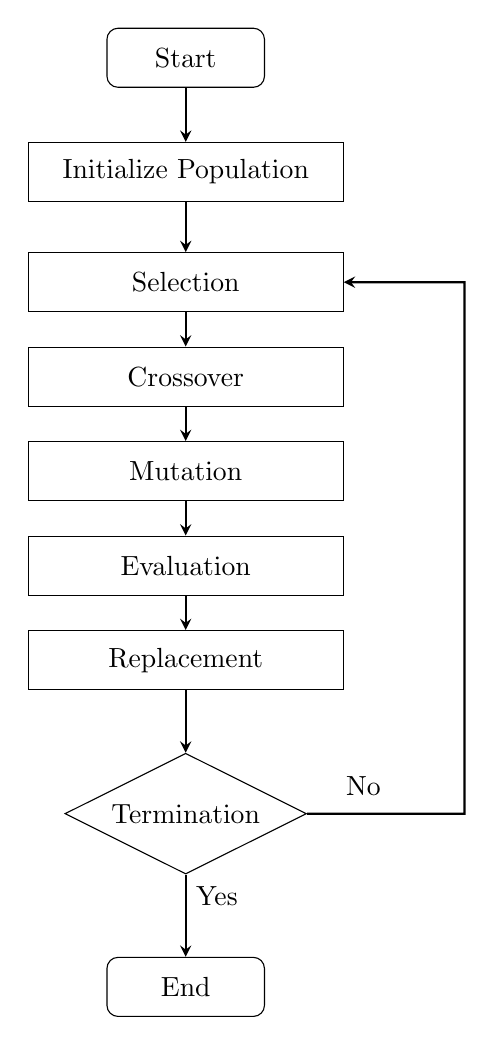
\begin{tikzpicture}[node distance=1.2cm]

    % Define styles for the nodes
    \tikzstyle{startstop} = [
        rectangle, rounded corners, text centered, draw=black,
        minimum width=2cm, minimum height=0.75cm
    ]
    \tikzstyle{process} = [
        rectangle, text centered, draw=black,
        minimum width=4cm, minimum height=0.75cm
    ]
    \tikzstyle{decision} = [
        diamond, text centered, draw=black,
        minimum width=3cm, minimum height=1cm, aspect=2
    ]
    \tikzstyle{arrow} = [thick,->,>=stealth]

    % Nodes
    \node (start) [startstop] {Start};
    \node (init) [process, below of=start, yshift=-0.25cm] {Initialize Population};
    \node (selection) [process, below of=init, yshift=-0.2cm] {Selection};
    \node (crossover) [process, below of=selection] {Crossover};
    \node (mutation) [process, below of=crossover] {Mutation};
    \node (evaluation) [process, below of=mutation] {Evaluation};
    \node (replacement) [process, below of=evaluation] {Replacement};
    \node (termination) [decision, below of=replacement, yshift=-0.75cm] {Termination};
    \node (end) [startstop, below of=termination, yshift=-1cm] {End};

    % Arrows
    \draw [arrow] (start) -- (init);
    \draw [arrow] (init) -- (selection);
    \draw [arrow] (selection) -- (crossover);
    \draw [arrow] (crossover) -- (mutation);
    \draw [arrow] (mutation) -- (evaluation);
    \draw [arrow] (evaluation) -- (replacement);
    \draw [arrow] (replacement) -- (termination);
    \draw [arrow] (termination.east) -- ++(2,0) |- ++(0,6.75cm) -- (selection.east) node [xshift=0.25cm, yshift=-6.4cm] {No};
    \draw [arrow] (termination) -- (end) node [midway, right, yshift=0.25cm] {Yes};

\end{tikzpicture}


    \caption{Flowchart of a generic genetic algorithm.}
    \label{fig:ga_flowchart}
\end{figure}


\subsection{Encoding Schemes}
Encoding defines how a genetic algorithm represents potential solutions to
the problem at hand \cite{Affenzeller2009}.
Depending on the approach, encoding schemes can be classified as direct or
indirect \cite{Thanh2007}.

In a direct encoding, the data structure used to represent a candidate solution
mirrors the problem's structure closely, meaning that the whole search space
is encoded \cite{Thanh2007,Goos2002}.
For example, in the context of timetabling, a direct encoding might use
matrices to map events directly to time slots and resources, providing a
straightforward representation that facilitates the evaluation of constraints.

In contrast, indirect encodings represent solutions in a more abstract form.
For instance, a permutation encoding might specify the sequence in which events
are scheduled, requiring additional processing -- such as a heuristic algorithm
-- to construct a complete timetable. While this approach offers greater
flexibility and may avoid certain constraint violations naturally, by clever
designed heuristics, it often demands additional computational resources for
constructing solutions.
One advantage of not encoding all information of a solution is, that
this can restrict the search space the algorithm has to explore \cite{Goos2002}

This distinction between the encoded data and its interpretation is described
by the terms genotype and phenotype \cite{Katoch2021}.
The genotype refers to the encoded representation manipulated by the genetic
operators, such as a list of binary values, a permutation of events, or another
abstract structure \cite{Affenzeller2009,Katoch2021}.
The phenotype, on the other hand, represents the decoded, problem-specific
solution used to evaluate objectives or constraints
\cite{Affenzeller2009,Katoch2021}.
For example, in timetabling, the genotype might consist of multiple lists
holding abstract information about a timetable, while the phenotype describes
the actual timetable derived from the abstract representation given by the
genotype.

% While a direct encoding simplifies the evaluation process by directly mapping
% the genotype to the phenotype, it often requires specialized genetic
% operators to maintain valid chromosomes. Indirect encodings, by contrast,
% can offer greater flexibility by leveraging heuristics to construct solutions
% from abstract representations, but this comes at the cost of additional
% computational effort.

% Despite the adaptability and potential of genetic algorithms, existing research
% in high-school timetabling suffers from notable limitations. Many studies fail
% to provide reproducible results, as their implementations are not made publicly
% available. Additionally, few studies leverage standardized problem instances,
% such as those provided by the XHSTT project, hindering meaningful comparisons
% between algorithms. Performance metrics, such as runtime or
% scalability, are also frequently underreported, leaving gaps in assessing
% algorithmic efficiency.


\subsection{Self-Parameterization}
A significant challenge in genetic algorithms lies in the process of parameter
tuning \cite{Katoch2021}.
Parameter tuning involves determining appropriate values for key variables such
mutation rates, population size, and elitism levels, but can also include
combining different genetic operators which work best for a given problem
instance.
This process often demands substantial computational resources, deep domain
expertise, and iterative experimentation.
Moreover, tuning parameters to optimize performance for a specific problem
instance can render the algorithm less generalizable, limiting its applicability
to diverse or unforeseen scenarios.

In educational timetabling, the issue is particularly pronounced, as the
diversity of problem instances requires a high degree of adaptability.
Traditional approaches to parameter tuning fail to address this variability,
often tailoring the algorithm so specifically that it becomes impractical for
general use or deployment in distributed software applications.

To address these challenges, adaptive evolutionary strategies offer a promising
alternative \cite{quaer2024survey}. Such strategies dynamically adjust the
algorithm's behavior during execution, based on metrics such as selection
pressure, population diversity or fitness convergence.
By leveraging real-time feedback, these adaptive mechanisms enable a degree of
self-parameterization, reducing reliance on manual tuning.

% Despite their potential, adaptive strategies remain underexplored in the context
% of high-school timetabling. Few studies integrate such methods into their
% frameworks, and even fewer provide implementation details necessary for
% reproducing the presented results. The algorithms developed in this thesis aim
% to address this gap by incorporating self-parameterization mechanisms.
% These mechanisms are analyzed for their impact on both runtime performance and
% solution quality, offering insights into how adaptive strategies can mitigate
% the parameter tuning problem while maintaining or improving the effectiveness
% of the search process.


\section{Methods}
This section outlines the methodologies and tools used in this thesis to explore
the effects of self-parameterization on genetic algorithms in high-school
timetabling. The approach focuses on flexibility, performance and
reproducibility, ensuring robust experimentation with a variety of encoding
schemes, genetic operators and parameterization methods.

\subsection{Framework}
To facilitate the extensive experimentation required for this thesis, a custom
framework was developed for implementing genetic algorithms. This framework
abstracts away the generic components of genetic algorithms, such as the
evolution loop, the implementation of selection mechanisms and population
management, allowing for rapid prototyping and testing of diverse
encoding schemes and self-parameterization strategies. By minimizing repetitive
implementation effort, the framework enables a streamlined focus on the unique
aspects of each genetic algorithm variation. Additionally, the framework
supports multithreaded execution and provides logging capabilities, making it
well-suited for both exploratory research and performance benchmarking.

\subsection{Programming Language}
The framework and all genetic algorithms were implemented in the Rust
programming language. Rust was chosen for several reasons:
\begin{itemize}
    \item   Performance and Efficiency: Rust code is compiled to native
            binaries, ensuring high runtime performance, which is crucial
            for computationally intensive tasks like solving timetabling
            problems.
    \item   Zero-cost Abstractions: Rust provides for ergonomic data modeling
            without incurring runtime overhead. This allows for clean and
            maintainable code that accurately represents the complex structures
            of timetabling.
    \item   Conditional Compilation: Its build system makes it easy to toggle
            parts of the code based on the requirements of a specific run.
            For example, while real-time metrics gathering can be enabled for
            detailed analysis during development, it can be disabled during
            benchmarking runs to maximize performance. Basic metrics, such as
            runtime or solution quality, can still be logged efficiently for
            post-analysis.
\end{itemize}


%%%%%%%%%%%%%%%%%%%%%%%%%%%%%%%%%%%%%%%%%%%%%%%%%%%%%%%%%%%%%%%%%%%%%%%%%%%%%%%%
%%% 3. Problem Representation                                                %%%
%%%%%%%%%%%%%%%%%%%%%%%%%%%%%%%%%%%%%%%%%%%%%%%%%%%%%%%%%%%%%%%%%%%%%%%%%%%%%%%%
\chapter{Problem Representation}
An effective problem representation is critical for the success of genetic
algorithms, as it defines how potential solutions are encoded and therefore
specifies how solution space is searched by the algorithm. This chapter
introduces the encoding schemes developed and used for this study, which form
the basis for the development of genetic algorithms.

%%%%%%%%%%%%%%%%%%%%%%%%%%%%
%%% 3.1. Direct Encoding %%%
%%%%%%%%%%%%%%%%%%%%%%%%%%%%
\section{Direct Encoding}
% Explanation of the direct encoding approach
In the context of the XHSTT format, solutions to timetable problems are
represented by allocations of time slots to events.
The direct encoding scheme therefore represents potential solution timetables
by associating a certain allocation of time slots with an event. With this
approach the encoding provides a straightforward and easily interpretable
representation of potential solutions. The following paragraphs describe the
key components of this direct encoding schema.

% Description of the genotype
\paragraph{Genotype}
As mentioned above, the direct encoding maintains a close relation between
the expected solution format and its genotype. This means that the genotype
represents a candidate solution timetable as a list of bit vectors. Each bit
vector corresponds to a specific event, identified by its index in the list.
The bit vector encodes the time slot allocation for the associated event,
with each bit indicating, if the event is scheduled at a certain time
or not. The time slots are thereby referenced by their index in the bit vector.
A set bit indicates that the event is allocated to the corresponding time slot,
while an unset bit indicates no allocation.
Figure \ref{fig:index_map} visualizes how times, events and resources
are mapped to indices, so that these indices can be used in the encoding for
referencing their counterparts, as it is shown in \ref{fig:direct_encoding}.

% Figure to show how the mapping of time, events and resources looks like.
\begin{figure}
    \centering
    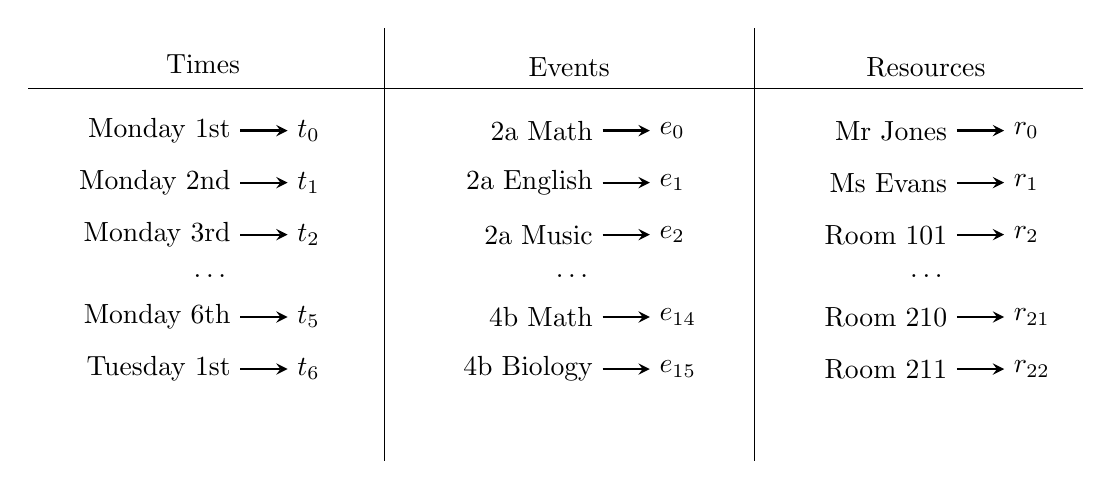
\begin{tikzpicture}[
    arrow/.style={-stealth, thick}, % Arrow style
    node distance=0.1cm and 0.6cm, auto,% Spacing between nodes
    textnode/.style={minimum width=2.3cm, text width=2.3cm, align=right}
]
    % Times column
    \node (t0) [textnode] at (0, 0)     {Monday 1st};
    \node (t1) [textnode, below= of t0] {Monday 2nd};
    \node (t2) [textnode, below= of t1] {Monday 3rd};
    \node (t3) [textnode, below= of t2] {\dots};
    \node (t5) [textnode, below= of t3] {Monday 6th};
    \node (t6) [textnode, below= of t5] {Tuesday 1st};

    % Events column
    \node (e0) [textnode, right of=t0, xshift=4.5cm]    {2a Math};
    \node (e1) [textnode, right of=t1, xshift=4.5cm]    {2a English};
    \node (e2) [textnode, right of=t2, xshift=4.5cm]    {2a Music};
    \node (e3) [textnode, right of=t3, xshift=4.5cm]    {\dots};
    \node (e5) [textnode, right of=t5, xshift=4.5cm]    {4b Math};
    \node (e6) [textnode, right of=t6, xshift=4.5cm]    {4b Biology};

    % Resources column
    \node (r0) [textnode, right of=t0, xshift=9cm]    {Mr Jones};
    \node (r1) [textnode, right of=t1, xshift=9cm]    {Ms Evans};
    \node (r2) [textnode, right of=t2, xshift=9cm]    {Room 101};
    \node (r3) [textnode, right of=t3, xshift=9cm]    {\dots};
    \node (r5) [textnode, right of=t5, xshift=9cm]    {Room 210};
    \node (r6) [textnode, right of=t6, xshift=9cm]    {Room 211};

    % Indices for times
    \node (ti0) [right= of t0] {$t_0$};
    \node (ti1) [right= of t1] {$t_1$};
    \node (ti2) [right= of t2] {$t_2$};
    \node (ti5) [right= of t5] {$t_5$};
    \node (ti6) [right= of t6] {$t_6$};

    % Indices for events
    \node (ei0) [right= of e0] {$e_0$};
    \node (ei1) [right= of e1] {$e_1$};
    \node (ei2) [right= of e2] {$e_2$};
    \node (ei5) [right= of e5] {$e_{14}$};
    \node (ei6) [right= of e6] {$e_{15}$};

    % Indices for resources
    \node (ri0) [right= of r0] {$r_0$};
    \node (ri1) [right= of r1] {$r_1$};
    \node (ri2) [right= of r2] {$r_2$};
    \node (ri5) [right= of r5] {$r_{21}$};
    \node (ri6) [right= of r6] {$r_{22}$};

    % Arrows for times
    \draw[arrow] (t0.east) -- (ti0.west);
    \draw[arrow] (t1.east) -- (ti1.west);
    \draw[arrow] (t2.east) -- (ti2.west);
    \draw[arrow] (t5.east) -- (ti5.west);
    \draw[arrow] (t6.east) -- (ti6.west);

    % Arrows for events
    \draw[arrow] (e0.east) -- (ei0.west);
    \draw[arrow] (e1.east) -- (ei1.west);
    \draw[arrow] (e2.east) -- (ei2.west);
    \draw[arrow] (e5.east) -- (ei5.west);
    \draw[arrow] (e6.east) -- (ei6.west);

    % Arrows for resources
    \draw[arrow] (r0.east) -- (ri0.west);
    \draw[arrow] (r1.east) -- (ri1.west);
    \draw[arrow] (r2.east) -- (ri2.west);
    \draw[arrow] (r5.east) -- (ri5.west);
    \draw[arrow] (r6.east) -- (ri6.west);

    % % Labels for columns
    \node[above=0.32cm of t0, xshift=0.8cm] {Times};
    \node[above=0.32cm of e0, xshift=0.85cm] {Events};
    \node[above=0.32cm of r0, xshift=0.88cm] {Resources};

    \draw (-1.42cm,0.54cm) -- ++(13.4,0);
    \draw (3.1cm,1.3cm) -- ++(0,-5.5cm);
    \draw (7.8cm,1.3cm) -- ++(0,-5.5cm);

\end{tikzpicture}


    \caption{
        Mapping times, events and resources to zero-based indices.
    }
    \label{fig:index_map}
\end{figure}

% Figure which visualizes the direct encoding schema.
\begin{figure}
    \centering
    \begin{tikzpicture}[
    every node/.style={align=center},
    bit0/.style={draw, minimum height=0.7cm, minimum width=0.7cm},
    bit1/.style={draw, minimum height=0.7cm, minimum width=0.7cm, fill=gray!20},
    event/.style={draw, minimum height=1.2cm, minimum width=1.2cm, text width=1cm},
    event2/.style={minimum height=1.2cm, minimum width=1.2cm, text width=1cm},
    arrow/.style={-stealth, thick} % Arrow style
]

    % Event indices (e_0, e_1, ...)
    \node[event] (e0) at (0, 0) {$e_0$};
    \node[event, below=0cm of e0] (e1) {$e_1$};
    \node[event, below=0cm of e1] (e2) {$e_2$};
    \node[event2, below=0cm of e2] (ex) {\dots};

    % Bit vectors (16 bits each)
    \node[bit0, right=1.2cm of e0] (b00) {0};
    \node[bit0, right=0cm of b00] (b01) {0};
    \node[bit1, right=0cm of b01] (b02) {1};
    \node[bit0, right=0cm of b02] (b03) {0};
    \node[bit0, right=0cm of b03] (b04) {0};
    \node[bit0, right=0cm of b04] (b05) {0};
    \node[bit0, right=0cm of b05] (b06) {0};
    \node[bit0, right=0cm of b06] (b07) {0};
    \node[bit0, right=0cm of b07] (b08) {0};
    \node[bit1, right=0cm of b08] (b09) {1};
    \node[bit0, right=0cm of b09] (b10) {0};
    \node[bit0, right=0cm of b10] (b11) {0};
    \node[bit0, right=0cm of b11] (b12) {0};
    \node[bit0, right=0cm of b12] (b13) {0};
    \node[bit1, right=0cm of b13] (b14) {1};
    \node[bit1, right=0cm of b14] (b15) {1};

    % Bit vector indices
    \node [above of=b15, yshift=-0.30cm] (i0) {$t_0$};
    \node [above of=b14, yshift=-0.30cm] (i1) {$t_1$};
    \node [above of=b13, yshift=-0.30cm] (i2) {$t_2$};
    \node [above of=b12, yshift=-0.30cm] (i3) {$t_3$};
    \node [above of=b11, yshift=-0.30cm] (i4) {$t_4$};
    \node [above of=b10, yshift=-0.30cm] (i5) {$t_5$};
    \node [above of=b09, yshift=-0.30cm] (i6) {$t_6$};
    \node [above of=b08, yshift=-0.30cm] (i7) {$t_7$};
    \node [above of=b07, yshift=-0.30cm] (i8) {$t_8$};
    \node [above of=b06, yshift=-0.30cm] (i9) {$t_9$};
    \node [above of=b05, yshift=-0.30cm] (i10) {$t_{10}$};
    \node [above of=b04, yshift=-0.30cm] (i11) {$t_{11}$};
    \node [above of=b03, yshift=-0.30cm] (i12) {$t_{12}$};
    \node [above of=b02, yshift=-0.30cm] (i13) {$t_{13}$};
    \node [above of=b01, yshift=-0.30cm] (i14) {$t_{14}$};
    \node [above of=b00, yshift=-0.30cm] (i15) {$t_{15}$};

    % Repeat for e_1
    \node[bit0, right=1.2cm of e1] (c00) {0};
    \node[bit0, right=0cm of c00] (c01) {0};
    \node[bit0, right=0cm of c01] (c02) {0};
    \node[bit0, right=0cm of c02] (c03) {0};
    \node[bit1, right=0cm of c03] (c04) {1};
    \node[bit0, right=0cm of c04] (c05) {0};
    \node[bit0, right=0cm of c05] (c06) {0};
    \node[bit0, right=0cm of c06] (c07) {0};
    \node[bit0, right=0cm of c07] (c08) {0};
    \node[bit1, right=0cm of c08] (c09) {1};
    \node[bit0, right=0cm of c09] (c10) {0};
    \node[bit0, right=0cm of c10] (c11) {0};
    \node[bit0, right=0cm of c11] (c12) {0};
    \node[bit1, right=0cm of c12] (c13) {1};
    \node[bit0, right=0cm of c13] (c14) {0};
    \node[bit0, right=0cm of c14] (c15) {0};

    % Repeat for e_2
    \node[bit0, right=1.2cm of e2] (d00) {0};
    \node[bit0, right=0cm of d00] (d01) {0};
    \node[bit1, right=0cm of d01] (d02) {1};
    \node[bit1, right=0cm of d02] (d03) {1};
    \node[bit0, right=0cm of d03] (d04) {0};
    \node[bit0, right=0cm of d04] (d05) {0};
    \node[bit0, right=0cm of d05] (d06) {0};
    \node[bit1, right=0cm of d06] (d07) {1};
    \node[bit1, right=0cm of d07] (d08) {1};
    \node[bit0, right=0cm of d08] (d09) {0};
    \node[bit0, right=0cm of d09] (d10) {0};
    \node[bit0, right=0cm of d10] (d11) {0};
    \node[bit1, right=0cm of d11] (d12) {1};
    \node[bit1, right=0cm of d12] (d13) {1};
    \node[bit0, right=0cm of d13] (d14) {0};
    \node[bit0, right=0cm of d14] (d15) {0};

    % Arrows connecting indices to bit vectors
    \draw[arrow] (e0.east) -- (b00.west);
    \draw[arrow] (e1.east) -- (c00.west);
    \draw[arrow] (e2.east) -- (d00.west);

    % Angle bracket for events
    \draw[decorate, decoration={brace, amplitude=10pt, mirror}, thick]
        ([xshift=-0.05cm, yshift=-0.34cm]ex.west)
            -- ([xshift=0.05cm, yshift=-0.34cm]ex.east)
        node[midway, below=12pt, font=\small]
        {corresponds to\\\lstinline[language=Rust]{Vec<...>} };

    % Angle bracket for bitvec
    \draw[decorate, decoration={brace, amplitude=10pt, mirror}, thick]
        ([xshift=-0.35cm, yshift=-1.2cm]d00.south)
            -- ([xshift=0.35cm, yshift=-1.2cm]d15.south)
        node[midway, below=12pt, font=\small]
        {corresponds to \lstinline[language=Rust]{Bits32} };

\end{tikzpicture}

    \caption{Visualization of the direct encoding data structure.}
    \label{fig:direct_encoding}
\end{figure}



The actual implementation of the genotype in code looks like this:
\begin{lstlisting}[language=Rust]
pub struct Chromosome(pub Vec<Bits32>);
\end{lstlisting}
This shows the previously mentioned list of bit vectors, where
\lstinline[language=Rust]{Bits32} is a custom bit vector implementation with
a maximum length of 32, leveraging low-level bit operations to be highly
efficient and optimize computational performance.

% Description of the phenotype and how it is derived from the genotype
\paragraph{Phenotype}
While the genotype encodes the structural representation of a solution, the
phenotype extends this functionality to enable constraint evaluation. In the
direct encoding, the phenotype comprises two main components: the time
allocation and the resource allocation matrix.

The time allocation component is identical to the genotype, representing the
allocation of time slots to events as a list of bit vectors. The resource
allocation matrix, on the other hand, is derived from the problem instance and
provides additional information about the resources required for each event.
The matrix uses bit vectors to indicate which resources (e.g. teachers, rooms,
etc.) are associated with which events.
For the selected problem instances chosen for this study, the resource
allocation is given in the problem definition. Therefore, the implementation
of the phenotype is realized as follows:
\begin{lstlisting}[language=Rust]
pub struct Phenotype {
    /// Time allocation (equal to the chromosome value)
    pub times: Vec<Bits32>,

    /// Resources matrix:
    /// - the outer vector represents the resources
    /// - the inner "bits" represent which events the resource is
    ///   allocated to
    pub resources: Vec<Bits64>,
}
\end{lstlisting}

As the genotype's time allocation is part of the phenotype and the resource
allocation is given by the problem instance, the phenotype
can easily be derived from a genotype, by copying the time allocation
information from the genotype to the phenotype.

Combining these two components, the phenotype provides the necessary
information to evaluate the feasibility of a candidate solution with respect to
the problem's constraints.

% Description of the evaluation of constraints with this encoding
\paragraph{Evaluation}
The previously mentioned problem instances \textit{hdtt4} and \textit{hdtt5}
only make use of the two constraints \textit{AssignTimeConstraint} and
\textit{AvoidClashesConstraint}, which in the context of the direct encoding
are evaluated as follows:

The \textit{AssignTimeConstraint} ensures the number of allocated time slots
for an event matches its duration. To evaluate this constraint, the
algorithm iterates through the time allocation bit vectors of each event,
counting the set bits. If the number of set bits matches the event's required
duration, the constraint is satisfied for that event. Any deviation contributes
to the overall cost of the solution, reflecting the degree to which this
constraint is violated.

Evaluating the \textit{AvoidClashesConstraint} -- which ensures that resources
like teachers or rooms are not double-booked at the same time -- is done by
iterating over all pairs of events that share a common resource in the
resource allocation matrix. For each pair, the algorithm checks for overlapping
time slot allocations by comparing the corresponding time allocation bit
vectors. If a conflict is found -- such as two events requiring the same teacher
at the same time -- a penalty cost is added. This check is computationally more
elaborate than the \textit{AssignTimeConstraint} but is crucial for ensuring
the feasibility of solutions.

% Describe the objective (minimizing the cost)
\paragraph{Objective}
The objective of the genetic algorithm in the context of the direct encoding
is to minimize the total cost associated with constraint violations. Solutions
with fewer violations are considered fitter, aligning with the principles of
evolutionary optimization.

%%%%%%%%%%%%%%%%%%%%%%%%%%%%%%
%%% 3.2. Indirect Encoding %%%
%%%%%%%%%%%%%%%%%%%%%%%%%%%%%%
\section{Indirect Encoding}
% Explanation of the direct encoding approach
In contrast to the direct encoding, the indirect encoding
approach represents solutions to the high-school timetabling problem in a more
abstract manner.
Although this abstraction increases the complexity of deriving a timetable from
the genotype, because it allows one genotype to represent a multitude of
timetables, it also offers optimization of the search process through the
solution space.
A heuristic is employed to identify the best of these timetables, which is then
selected as the representative of the genotype.
This effectively enhances the search performance, as the heuristic eliminates
less optimal timetables.
%
This section explains the genotype and phenotype used in the indirect encoding,
details the heuristic employed for the phenotype derivation and outlines the
evaluation process as well as the optimization objective.

% Description of the genotype
\paragraph{Genotype}
The genotype in the indirect encoding represents a potential solution as a
permutation of event indices. This representation abstracts away direct time
slot allocations, encoding only the order in which events should be scheduled.
The implementation of this genotype is defined as:
\begin{lstlisting}[language=Rust]
pub struct Chromosome(pub Vec<u8>);
\end{lstlisting}

Here, each entry in the \lstinline[language=Rust]{Vec<u8>} corresponds to an
event index. The indices are unique and appear exactly once, ensuring the
genotype encodes a permutation of events.
This encoding scheme eliminates the need to explicitly allocate time slots
during the evolutionary search phase, delegating the actual scheduling process
to a heuristic that constructs the actual timetable by deriving a phenotype
from the genotype.

% Description of the phenotype and how it is derived from the genotype
\paragraph{Phenotype}
The phenotype provides a derivation logic, to construct itself from a given
genotype, as well as the necessary data structures to perform constraint
evaluation. It comprises two key components,
\lstinline[language=Rust]|times| and \lstinline[language=Rust]|blocked|:
\begin{lstlisting}[language=Rust]
pub struct Phenotype {
    /// The `times` matrix represents the allocation of times to
    /// events.
    pub times: BitsMatrix32x128,

    /// The `blocked` matrix tracks timeslots that are
    /// unavailable for scheduling.
    pub blocked: BitsMatrix32x128,
}
\end{lstlisting}

The \lstinline[language=Rust]|times| matrix encodes the time slots allocated
to each event, similar to the structure used in the direct encoding. However,
the indirect encoding adds a \lstinline[language=Rust]|blocked| matrix, which
tracks time slots unavailable for scheduling due to resource constraints imposed
by previously scheduled events. Opposed to the direct encoding, the indirect
encoding does not use vector data structures but rather bit matrices, which are
-- similar to the custom bit vectors -- custom implementations to improve
computational efficiency. They have been specifically implemented to be used
in the indirect encoding, because of the increased complexity of this encoding
scheme in comparison to the direct encoding.

The phenotype's data structure does not directly contain information about
resource allocations anymore. Instead, this data is accessed via the context,
a central data structure containing a set of important information and
parameters, which is used throughout the whole algorithm. For the derivation
process of the phenotype, the context provides a pre-computed list of
so-called \textit{collision vectors}. Each of these collision vectors
corresponds to an event and holds information about related events, which
have resources in common with the given event. The collision vectors for each
event can be calculated from the resource allocation data which is provided by
XHSTT problem instances like \textit{hdtt4} and \textit{hdtt5}. As the
collision vectors are needed in every derivation, they are initially
calculated and stored in the forementioned context, which is then provided to
the derivation algorithm.
%
Figure \ref{fig:pre_calc_collision_vec} illustrates the calculation of a
collision vector for a given event. The process works by first inspecting the
given event's resources and then extracting the other events these resources
are needed for. All these events are then collected into one vector yielding
the collision vector for the given event.
%
% Visualization of the pre-calculation of the collision vectors.
\begin{figure}
    \centering
    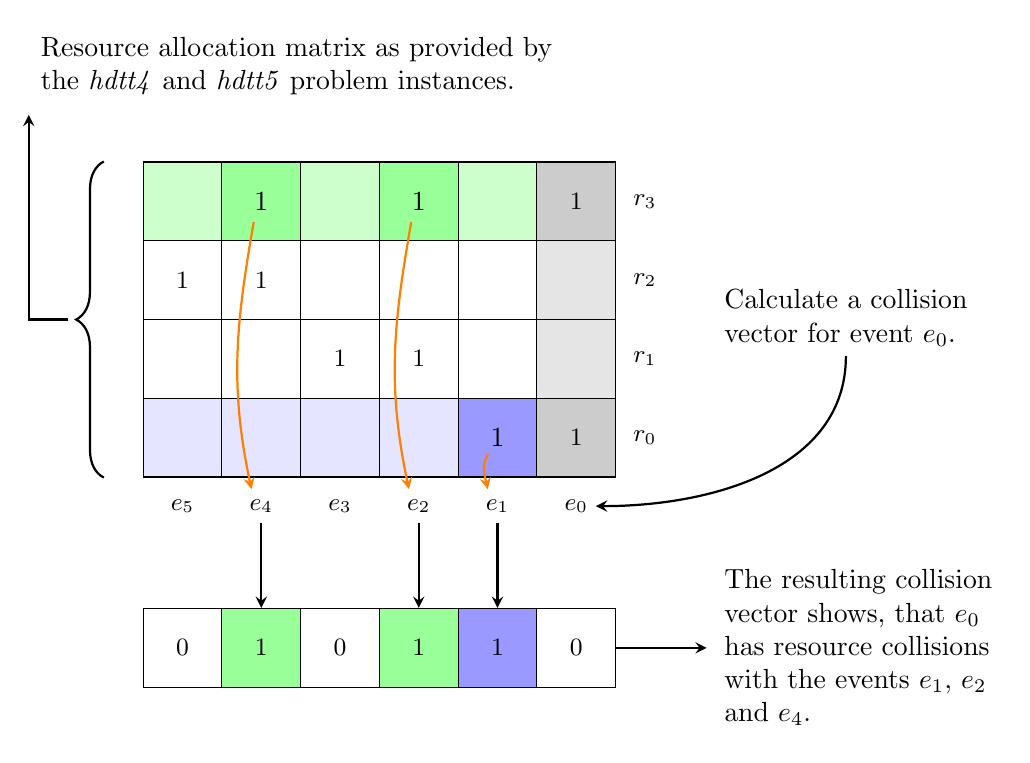
\begin{tikzpicture}[
    cell/.style={draw, minimum size=1cm, font=\small},
    label/.style={font=\small, align=center},
    arrow/.style={-stealth, thick},
    desc/.style={align=left}
]
    % Matrix dimensions
    \def\rows{4}
    \def\cols{6}

    % r0
    \node [cell, fill=gray!40] (e0r0) at (-0, 0) {1};
    \node [cell, fill=blue!40] (e1r0) at (-1, 0) {};
        \node (e1r0_text) at (-1, 0) {1};
    \node [cell, fill=blue!10] (e2r0) at (-2, 0) {};
    \node [cell, fill=blue!10] (e3r0) at (-3, 0) {};
    \node [cell, fill=blue!10] (e4r0) at (-4, 0) {};
    \node [cell, fill=blue!10] (e5r0) at (-5, 0) {};

    % r1
    \node [cell, fill=gray!20] (e0r1) at (-0, 1) {};
    \node [cell] (e1r1) at (-1, 1) {};
    \node [cell] (e2r1) at (-2, 1) {1};
    \node [cell] (e3r1) at (-3, 1) {1};
    \node [cell] (e4r1) at (-4, 1) {};
    \node [cell] (e5r1) at (-5, 1) {};

    % r2
    \node [cell, fill=gray!20] (e0r2) at (-0, 2) {};
    \node [cell] (e1r2) at (-1, 2) {};
    \node [cell] (e2r2) at (-2, 2) {};
    \node [cell] (e3r2) at (-3, 2) {};
    \node [cell] (e4r2) at (-4, 2) {1};
    \node [cell] (e5r2) at (-5, 2) {1};

    % r3
    \node [cell, fill=gray!40] (e0r3) at (-0, 3) {1};
    \node [cell, fill=green!20] (e1r3) at (-1, 3) {};
    \node [cell, fill=green!40] (e2r3) at (-2, 3) {};
        \node (e2r3_text) at (-2, 3) {1};
    \node [cell, fill=green!20] (e3r3) at (-3, 3) {};
    \node [cell, fill=green!40] (e4r3) at (-4, 3) {};
        \node (e4r3_text) at (-4, 3) {1};
    \node [cell, fill=green!20] (e5r3) at (-5, 3) {};

    % Add row labels (r_0, r_1, ..., r_3)
    \foreach \row in {0,...,3} {
        \node[label, right=0.60cm] at (0, \row) {$r_{\row}$};
    }

    % Add column labels (e_0, e_1, ..., e_5)
    \foreach \col [count=\x from 0] in {5,...,0} {
        \node[label, below=0.16cm] (e_\x) at (-\x, -0.5) {$e_{\x}$};
    }


    % Arrows from ones to the their corresponding event index.
    \draw[arrow, orange]
        ([shift={(240:0.24cm)}]e1r0_text.center)
        to[out=240, in=102]
        ([shift={(120:0.25cm)}]e_1.center);

    \draw[arrow, orange]
        ([shift={(250:0.28cm)}]e2r3_text.center)
        to[out=260, in=102]
        ([shift={(120:0.25cm)}]e_2.center);

    \draw[arrow, orange]
        ([shift={(250:0.28cm)}]e4r3_text.center)
        to[out=260, in=102]
        ([shift={(120:0.25cm)}]e_4.center);

    % Description text
    \node [desc, right=of e0r2, xshift=0.25cm, yshift=-0.48cm] (desc_text) {
        Calculate a collision\\
        vector for event $e_0$.
    };

    \draw[arrow]
        ([shift={(270:0.0cm)}]desc_text.south)
        to[out=270, in=0]
        ([shift={(0:0.25cm)}]e_0.center);

    % Resulting collision vector
    \node [cell, below of=e_0, yshift=-0.8cm] (cv0) {0};
    \node [cell, below of=e_1, yshift=-0.8cm, fill=blue!40] (cv1) {1};
    \node [cell, below of=e_2, yshift=-0.8cm, fill=green!40] (cv2) {1};
    \node [cell, below of=e_3, yshift=-0.8cm] (cv3) {0};
    \node [cell, below of=e_4, yshift=-0.8cm, fill=green!40] (cv4) {1};
    \node [cell, below of=e_5, yshift=-0.8cm] (cv5) {0};

    \draw[arrow] (e_1) -- (cv1);
    \draw[arrow] (e_2) -- (cv2);
    \draw[arrow] (e_4) -- (cv4);

    % Collision Vector Description
    \node [desc, right=of cv0, xshift=0.25cm] (desc_cv) {
        The resulting collision\\
        vector shows, that $e_0$\\
        has resource collisions\\
        with the events $e_1$, $e_2$\\
        and $e_4$.
    };

    \draw[arrow]
        ([shift={(0:0.0cm)}]cv0.east)
        --
        ([shift={(180:0.1cm)}]desc_cv.west);

    % Angle bracket for resource allocation matrix
    \draw[decorate, decoration={brace, amplitude=10pt, mirror}, thick]
        ([xshift=-1.0cm]e5r3.north)
        --
        ([xshift=-1.0cm]e5r0.south)
            node[midway, align=center, left=12pt] (bracket) {};

    % Description of the resource allocation matrix
    \node[desc, align=left, above=of bracket, xshift=3cm, yshift=1.6cm]
        (resource_matrix_desc)
    {
        Resource allocation matrix as provided by\\the \textit{hdtt4} and
        \textit{hdtt5} problem instances.
    };

    \draw[arrow]
        ([shift={(0.1cm,0)}]bracket.center)
        -- ++(-0.5cm, 0cm)
        -- ++(0cm, 2.6cm);

\end{tikzpicture}

    \caption{Illustration of calculating a collision vector and its meaning.}
    \label{fig:pre_calc_collision_vec}
\end{figure}
%
The resulting collision vectors are stored as a list of bit vectors on the
context as shown below:
\begin{lstlisting}[language=Rust]
pub struct Context {
    /// Collision vectors.
    pub resource_relations: Vec<Bits128>,
    ...
}
\end{lstlisting}


% Derivation process (=> this is where the heuristic needs to be explained)
With the collision vectors pre-calculated, the heuristic algorithm can now start
to translate the order of events specified by the genotype into a fully
defined timetable. This process involves iterating through the genotype and
scheduling each event in the specified order. The heuristic operates as follows:

First, for each event, the heuristic selects a fixed number of random time slot
combinations. Each combination contains a number of time slots that matches the
event's required duration.
The heuristic algorithm then simulates scheduling each of those time slot
combinations, checking for conflicts using the
\lstinline[language=Rust]|times| matrix, to ensure it does not overlap with
previously scheduled events.
%
For valid combinations, a fitness metric is
computed, favoring those that minimize additional blocked time slots.
This translates to favoring combinations that block already-blocked time slots,
as this indicates efficient allocation of resources.
%
The data needed for this evaluation is provided by the
\lstinline[language=Rust]|blocked| matrix.
Lastly, the combination with the highest rank is applied, updating both the
\lstinline[language=Rust]|times| and \lstinline[language=Rust]|blocked|
matrices of the phenotype. If no valid combination exists, the event remains
unscheduled, ensuring that no resource conflicts are introduced. This process
is visualized in example \ref{ex:heuristic_example}.

This scheduling process continues until all events have been processed. By
design, the heuristic guarantees that no resource conflicts arise, eliminating
the need to evaluate the \textit{AvoidClashesConstraint} during the
constraint evaluation phase.

% Description of the evaluation of constraints with this encoding
\paragraph{Evaluation}
As the heuristic ensures the absence of resource conflicts, only the
\textit{AssignTimeConstraint} must be evaluated. The evaluation process
involves counting the number of time slots allocated to each event in the
\lstinline[language=Rust]|times| matrix. If the number of allocated time slots
matches the event's required duration, no penalty is incurred. If the number
deviates from the required duration, a penalty cost proportional to the
violation is added. The total accumulated cost represents the cost (or fitness)
of the solution timetable.

% Describe the objective (minimizing the cost)
\paragraph{Objective}
Similar to the direct encoding, the objective of the genetic algorithm
is to minimize the total cost associated with constraint violations. A solution
with zero cost represents a valid timetable with no constraint violations.

\begin{minipage}{\textwidth}
    \begin{Example}[Heuristic process with efficiency evaluation]
        \begin{minipage}{\textwidth}
            \centering
            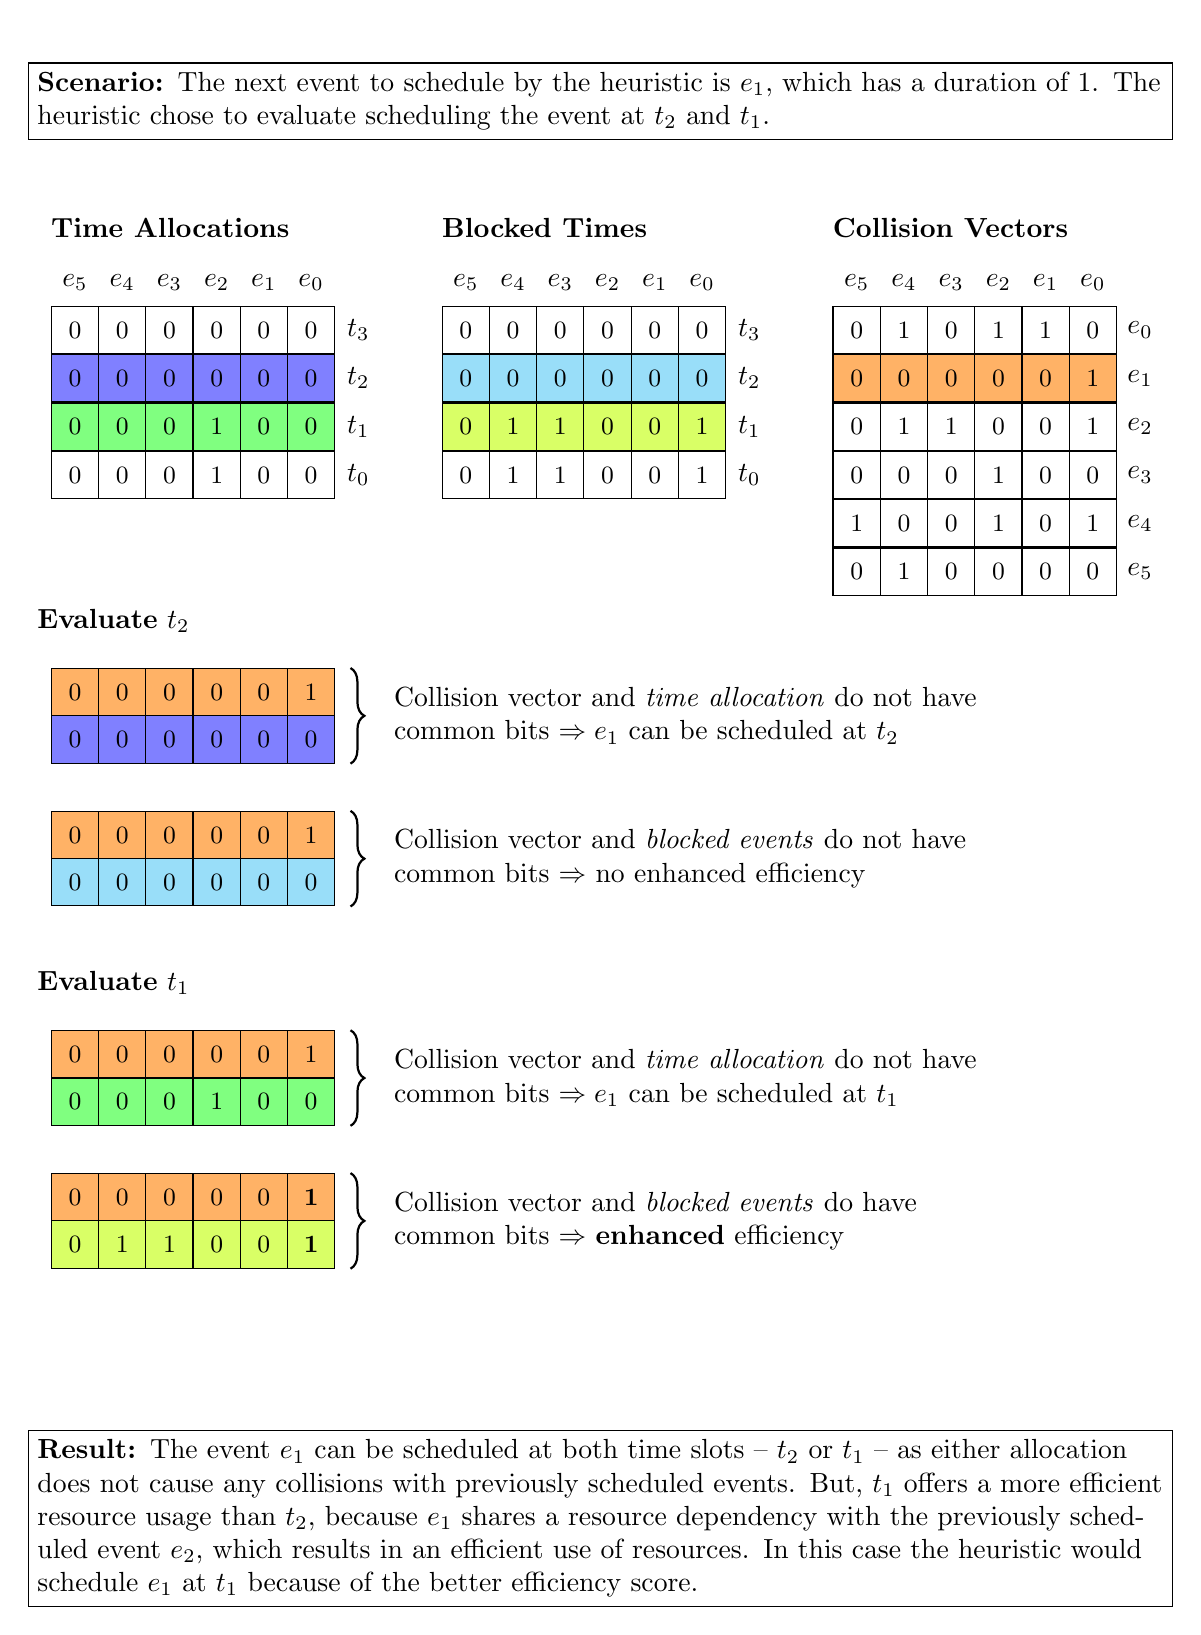
\begin{tikzpicture}[
    node distance = 0.6cm,
    cell/.style={draw, minimum size=0.6cm, font=\small},
    % label/.style={font=\small, align=center},
    % arrow/.style={-stealth, thick},
    desc/.style={align=left, text width=14.3cm},
]
    \node(top_spacer) [] {};
    \node[desc, draw, below=0.2cm of top_spacer] (example_desc) {
        \textbf{Scenario:} The next event to schedule by the heuristic
        is $e_1$, which has a duration of $1$. The heuristic chose to
        evaluate scheduling the event at $t_2$ and $t_1$.
    };

    % Times matrix
    \node[cell, below=of example_desc.west, xshift=0.6cm, yshift=-2cm] (t3e5) {0};
    \node[cell, right of=t3e5]          (t3e4) {0};
    \node[cell, right of=t3e4]          (t3e3) {0};
    \node[cell, right of=t3e3]          (t3e2) {0};
    \node[cell, right of=t3e2]          (t3e1) {0};
    \node[cell, right of=t3e1]          (t3e0) {0};

    \node[cell, below=0cm of t3e5, fill=blue!50]      (t2e5) {0};
    \node[cell, right of=t2e5, fill=blue!50]          (t2e4) {0};
    \node[cell, right of=t2e4, fill=blue!50]          (t2e3) {0};
    \node[cell, right of=t2e3, fill=blue!50]          (t2e2) {0};
    \node[cell, right of=t2e2, fill=blue!50]          (t2e1) {0};
    \node[cell, right of=t2e1, fill=blue!50]          (t2e0) {0};

    \node[cell, below=0cm of t2e5, fill=green!50]      (t1e5) {0};
    \node[cell, right of=t1e5, fill=green!50]          (t1e4) {0};
    \node[cell, right of=t1e4, fill=green!50]          (t1e3) {0};
    \node[cell, right of=t1e3, fill=green!50]          (t1e2) {1};
    \node[cell, right of=t1e2, fill=green!50]          (t1e1) {0};
    \node[cell, right of=t1e1, fill=green!50]          (t1e0) {0};

    \node[cell, below=0cm of t1e5]      (t0e5) {0};
    \node[cell, right of=t0e5]          (t0e4) {0};
    \node[cell, right of=t0e4]          (t0e3) {0};
    \node[cell, right of=t0e3]          (t0e2) {1};
    \node[cell, right of=t0e2]          (t0e1) {0};
    \node[cell, right of=t0e1]          (t0e0) {0};

    % Times matrix indices -> event
    \node[above of=t3e5] (t_e5) {$e_5$};
    \node[above of=t3e4] (t_e4) {$e_4$};
    \node[above of=t3e3] (t_e3) {$e_3$};
    \node[above of=t3e2] (t_e2) {$e_2$};
    \node[above of=t3e1] (t_e1) {$e_1$};
    \node[above of=t3e0] (t_e0) {$e_0$};

    % Times matrix indices -> time
    \node[right of=t3e0] (t_t3) {$t_3$};
    \node[right of=t2e0] (t_t2) {$t_2$};
    \node[right of=t1e0] (t_t1) {$t_1$};
    \node[right of=t0e0] (t_t0) {$t_0$};


    % Blocked matrix
    \node[cell, right=of t3e0, xshift=0.75cm] (b3e5) {0};
    \node[cell, right of=b3e5]          (b3e4) {0};
    \node[cell, right of=b3e4]          (b3e3) {0};
    \node[cell, right of=b3e3]          (b3e2) {0};
    \node[cell, right of=b3e2]          (b3e1) {0};
    \node[cell, right of=b3e1]          (b3e0) {0};

    \node[cell, below=0cm of b3e5, fill=cyan!40]      (b2e5) {0};
    \node[cell, right of=b2e5, fill=cyan!40]          (b2e4) {0};
    \node[cell, right of=b2e4, fill=cyan!40]          (b2e3) {0};
    \node[cell, right of=b2e3, fill=cyan!40]          (b2e2) {0};
    \node[cell, right of=b2e2, fill=cyan!40]          (b2e1) {0};
    \node[cell, right of=b2e1, fill=cyan!40]          (b2e0) {0};

    \node[cell, below=0cm of b2e5, fill=lime!60]      (b1e5) {0};
    \node[cell, right of=b1e5, fill=lime!60]          (b1e4) {1};
    \node[cell, right of=b1e4, fill=lime!60]          (b1e3) {1};
    \node[cell, right of=b1e3, fill=lime!60]          (b1e2) {0};
    \node[cell, right of=b1e2, fill=lime!60]          (b1e1) {0};
    \node[cell, right of=b1e1, fill=lime!60]          (b1e0) {1};

    \node[cell, below=0cm of b1e5]      (b0e5) {0};
    \node[cell, right of=b0e5]          (b0e4) {1};
    \node[cell, right of=b0e4]          (b0e3) {1};
    \node[cell, right of=b0e3]          (b0e2) {0};
    \node[cell, right of=b0e2]          (b0e1) {0};
    \node[cell, right of=b0e1]          (b0e0) {1};

    % Blocked matrix indices -> event
    \node[above of=b3e5] (b_e5) {$e_5$};
    \node[above of=b3e4] (b_e4) {$e_4$};
    \node[above of=b3e3] (b_e3) {$e_3$};
    \node[above of=b3e2] (b_e2) {$e_2$};
    \node[above of=b3e1] (b_e1) {$e_1$};
    \node[above of=b3e0] (b_e0) {$e_0$};

    % Blocked matrix indices -> time
    \node[right of=b3e0] (b_t3) {$t_3$};
    \node[right of=b2e0] (b_t2) {$t_2$};
    \node[right of=b1e0] (b_t1) {$t_1$};
    \node[right of=b0e0] (b_t0) {$t_0$};


    % Collision matrix
    \node[cell, right=of b3e0, xshift=0.75cm] (e0e5) {0};
    \node[cell, right of=e0e5]          (e0e4) {1};
    \node[cell, right of=e0e4]          (e0e3) {0};
    \node[cell, right of=e0e3]          (e0e2) {1};
    \node[cell, right of=e0e2]          (e0e1) {1};
    \node[cell, right of=e0e1]          (e0e0) {0};

    \node[cell, below=0cm of e0e5, fill=orange!60]      (e1e5) {0};
    \node[cell, right of=e1e5, fill=orange!60]          (e1e4) {0};
    \node[cell, right of=e1e4, fill=orange!60]          (e1e3) {0};
    \node[cell, right of=e1e3, fill=orange!60]          (e1e2) {0};
    \node[cell, right of=e1e2, fill=orange!60]          (e1e1) {0};
    \node[cell, right of=e1e1, fill=orange!60]          (e1e0) {1};

    \node[cell, below=0cm of e1e5]      (e2e5) {0};
    \node[cell, right of=e2e5]          (e2e4) {1};
    \node[cell, right of=e2e4]          (e2e3) {1};
    \node[cell, right of=e2e3]          (e2e2) {0};
    \node[cell, right of=e2e2]          (e2e1) {0};
    \node[cell, right of=e2e1]          (e2e0) {1};

    \node[cell, below=0cm of e2e5]      (e3e5) {0};
    \node[cell, right of=e3e5]          (e3e4) {0};
    \node[cell, right of=e3e4]          (e3e3) {0};
    \node[cell, right of=e3e3]          (e3e2) {1};
    \node[cell, right of=e3e2]          (e3e1) {0};
    \node[cell, right of=e3e1]          (e3e0) {0};

    \node[cell, below=0cm of e3e5]      (e4e5) {1};
    \node[cell, right of=e4e5]          (e4e4) {0};
    \node[cell, right of=e4e4]          (e4e3) {0};
    \node[cell, right of=e4e3]          (e4e2) {1};
    \node[cell, right of=e4e2]          (e4e1) {0};
    \node[cell, right of=e4e1]          (e4e0) {1};

    \node[cell, below=0cm of e4e5]      (e5e5) {0};
    \node[cell, right of=e5e5]          (e5e4) {1};
    \node[cell, right of=e5e4]          (e5e3) {0};
    \node[cell, right of=e5e3]          (e5e2) {0};
    \node[cell, right of=e5e2]          (e5e1) {0};
    \node[cell, right of=e5e1]          (e5e0) {0};

    % Collision vectors indices -> event
    \node[above of=e0e5] (e_e5) {$e_5$};
    \node[above of=e0e4] (e_e4) {$e_4$};
    \node[above of=e0e3] (e_e3) {$e_3$};
    \node[above of=e0e2] (e_e2) {$e_2$};
    \node[above of=e0e1] (e_e1) {$e_1$};
    \node[above of=e0e0] (e_e0) {$e_0$};

    \node[right of=e0e0] (e_e0_2) {$e_0$};
    \node[right of=e1e0] (e_e1_2) {$e_1$};
    \node[right of=e2e0] (e_e2_2) {$e_2$};
    \node[right of=e3e0] (e_e3_2) {$e_3$};
    \node[right of=e4e0] (e_e4_2) {$e_4$};
    \node[right of=e5e0] (e_e5_2) {$e_5$};

    % Matrix title
    \node[right=0cm of t_e5.west, xshift=-0.14cm, yshift=0.7cm] {
        \textbf{Time Allocations}
    };
    \node[right=0cm of b_e5.west, xshift=-0.14cm, yshift=0.7cm] {
        \textbf{Blocked Times}
    };
    \node[right=0cm of e_e5.west, xshift=-0.14cm, yshift=0.7cm] {
        \textbf{Collision Vectors}
    };


    % Evaluate t2
    \node[desc, below of=example_desc, yshift=-6.0cm] (eval_t2_desc) {
        \textbf{Evaluate $t_2$}
    };

    % Collision vector
    \node[cell, below=of eval_t2_desc.west, xshift=0.6cm, fill=orange!60] (cv5_1) {0};
    \node[cell, right of=cv5_1, fill=orange!60] (cv4_1) {0};
    \node[cell, right of=cv4_1, fill=orange!60] (cv3_1) {0};
    \node[cell, right of=cv3_1, fill=orange!60] (cv2_1) {0};
    \node[cell, right of=cv2_1, fill=orange!60] (cv1_1) {0};
    \node[cell, right of=cv1_1, fill=orange!60] (cv0_1) {1};

    % Times row
    \node[cell, below of=cv5_1, fill=blue!50] (tr5) {0};
    \node[cell, below of=cv4_1, fill=blue!50] (tr4) {0};
    \node[cell, below of=cv3_1, fill=blue!50] (tr3) {0};
    \node[cell, below of=cv2_1, fill=blue!50] (tr2) {0};
    \node[cell, below of=cv1_1, fill=blue!50] (tr1) {0};
    \node[cell, below of=cv0_1, fill=blue!50] (tr0) {0};

    \draw[decorate, decoration={brace, amplitude=5pt}, thick]
        ([xshift=0.5cm]cv0_1.north)
        --
        ([xshift=0.5cm]tr0.south)
            node[midway, align=left, right=12pt] (bracket)
        {
            Collision vector and \textit{time allocation} do not have\\
            common bits
            $\Rightarrow e_1$ can be scheduled at $t_2$
        };

    % Collision vector
    \node[cell, below=of tr5,   fill=orange!60] (cv5_2) {0};
    \node[cell, right of=cv5_2, fill=orange!60] (cv4_2) {0};
    \node[cell, right of=cv4_2, fill=orange!60] (cv3_2) {0};
    \node[cell, right of=cv3_2, fill=orange!60] (cv2_2) {0};
    \node[cell, right of=cv2_2, fill=orange!60] (cv1_2) {0};
    \node[cell, right of=cv1_2, fill=orange!60] (cv0_2) {1};

    % Blocked row
    \node[cell, below of=cv5_2, fill=cyan!40] (br5) {0};
    \node[cell, below of=cv4_2, fill=cyan!40] (br4) {0};
    \node[cell, below of=cv3_2, fill=cyan!40] (br3) {0};
    \node[cell, below of=cv2_2, fill=cyan!40] (br2) {0};
    \node[cell, below of=cv1_2, fill=cyan!40] (br1) {0};
    \node[cell, below of=cv0_2, fill=cyan!40] (br0) {0};

    \draw[decorate, decoration={brace, amplitude=5pt}, thick]
        ([xshift=0.5cm]cv0_2.north)
        --
        ([xshift=0.5cm]br0.south)
            node[midway, align=left, right=12pt] (bracket)
        {
            Collision vector and \textit{blocked events} do not have\\
            common bits
            $\Rightarrow$ no enhanced efficiency
        };


    % Evaluate t1
    \node[desc, below of=eval_t2_desc, yshift=-4cm] (eval_t1_desc) {
        \textbf{Evaluate $t_1$}
    };

    % Collision vector
    \node[cell, below=of eval_t1_desc.west, xshift=0.6cm, fill=orange!60] (cv5_3) {0};
    \node[cell, right of=cv5_3, fill=orange!60] (cv4_3) {0};
    \node[cell, right of=cv4_3, fill=orange!60] (cv3_3) {0};
    \node[cell, right of=cv3_3, fill=orange!60] (cv2_3) {0};
    \node[cell, right of=cv2_3, fill=orange!60] (cv1_3) {0};
    \node[cell, right of=cv1_3, fill=orange!60] (cv0_3) {1};

    % Times row
    \node[cell, below of=cv5_3, fill=green!50] (tr5_1) {0};
    \node[cell, below of=cv4_3, fill=green!50] (tr4_1) {0};
    \node[cell, below of=cv3_3, fill=green!50] (tr3_1) {0};
    \node[cell, below of=cv2_3, fill=green!50] (tr2_1) {1};
    \node[cell, below of=cv1_3, fill=green!50] (tr1_1) {0};
    \node[cell, below of=cv0_3, fill=green!50] (tr0_1) {0};

    \draw[decorate, decoration={brace, amplitude=5pt}, thick]
        ([xshift=0.5cm]cv0_3.north)
        --
        ([xshift=0.5cm]tr0_1.south)
            node[midway, align=left, right=12pt] (bracket)
        {
            Collision vector and \textit{time allocation} do not have\\
            common bits
            $\Rightarrow e_1$ can be scheduled at $t_1$
        };

    % Collision vector
    \node[cell, below=of tr5_1, fill=orange!60] (cv5_4) {0};
    \node[cell, right of=cv5_4, fill=orange!60] (cv4_4) {0};
    \node[cell, right of=cv4_4, fill=orange!60] (cv3_4) {0};
    \node[cell, right of=cv3_4, fill=orange!60] (cv2_4) {0};
    \node[cell, right of=cv2_4, fill=orange!60] (cv1_4) {0};
    \node[cell, right of=cv1_4, fill=orange!60] (cv0_4) {\textbf{1}};

    % Blocked row
    \node[cell, below of=cv5_4, fill=lime!60] (br5_1) {0};
    \node[cell, below of=cv4_4, fill=lime!60] (br4_1) {1};
    \node[cell, below of=cv3_4, fill=lime!60] (br3_1) {1};
    \node[cell, below of=cv2_4, fill=lime!60] (br2_1) {0};
    \node[cell, below of=cv1_4, fill=lime!60] (br1_1) {0};
    \node[cell, below of=cv0_4, fill=lime!60] (br0_1) {\textbf{1}};

    \draw[decorate, decoration={brace, amplitude=5pt}, thick]
        ([xshift=0.5cm]cv0_4.north)
        --
        ([xshift=0.5cm]br0_1.south)
            node[midway, align=left, right=12pt] (bracket)
        {
            Collision vector and \textit{blocked events} do have\\
            common bits
            $\Rightarrow$ \textbf{enhanced} efficiency
        };

    % Result
    \node[desc, draw, below of=eval_t1_desc, yshift=-6.2cm] {
        \textbf{Result:} The event $e_1$ can be scheduled at both time
        slots -- $t_2$ or $t_1$ -- as either allocation does not cause any
        collisions with previously scheduled events.
        But, $t_1$ offers a more efficient resource usage than $t_2$,
        because $e_1$ shares a resource dependency with the previously
        scheduled event $e_2$, which results in an efficient use of
        resources.
        In this case the heuristic would schedule $e_1$ at $t_1$ because of
        the better efficiency score.
    };

\end{tikzpicture}

            \label{ex:heuristic_example}
        \end{minipage}
    \end{Example}
\end{minipage}



%%%%%%%%%%%%%%%%%%%%%%%%%%%%%%%%%%%%%%%%%%%%%%%%%%%%%%%%%%%%%%%%%%%%%%%%%%%%%%%%
%%% 4. Genetic Algorithm                                                     %%%
%%%%%%%%%%%%%%%%%%%%%%%%%%%%%%%%%%%%%%%%%%%%%%%%%%%%%%%%%%%%%%%%%%%%%%%%%%%%%%%%
\chapter{Genetic Algorithm}
This chapter describes the genetic algorithms developed for this study, focusing
on their structure, special features and the genetic operators they employ.
The genetic algorithms implemented in this study follow the general process
of genetic search, known from textbooks and related research, which was
introduced earlier \cite{goldberg1989}.
%
To enable flexibility and efficiency during development, a dedicated framework
was created, which facilitates the implementation of new genetic algorithms
and provides tools for real-time analysis and capturing metrics. The following
sections outline how genetic algorithms work in general, what the framework
adds to that and describes details of the genetic operators.


%%%%%%%%%%%%%%%%%%%%%%%%%%%%%%
%%% 4.1. Generic Framework %%%
%%%%%%%%%%%%%%%%%%%%%%%%%%%%%%
\section{Generic Framework for Genetic Algorithms}
\label{Generic Framework for Genetic Algorithms}
To support the development of genetic algorithms, a generic framework was
designed and implemented. This framework abstracts the genetic search process
and provides essential features that enable rapid prototyping and
experimentation. By implementing predefined interfaces, users of the framework
can focus on developing the encoding and specific genetic operators, while the
framework handles the overall workflow of the genetic algorithm.
Key features of the framework include:
\begin{itemize}
    \item   \textbf{Interface-Based Design:} The framework defines clear
            interfaces for essential genetic operations such as selection,
            crossover, mutation and evaluation. By implementing these
            interfaces, developers have the freedom to implement custom
            encodings and still leverage the conveniences of the framework.

    \item   \textbf{Multi-Threading:} To improve computational efficiency, the
            framework supports multithreaded execution, enabling
            parallelization to reduce runtime.

    \item   \textbf{Logging and Metrics Collection:} During runtime, the
            framework captures detailed logs and performance metrics, including
            population statistics, operator behavior, and fitness trends.
            These data enable in-depth analysis of algorithm behavior and
            facilitate post-experiment evaluations.

    \item   \textbf{Predefined Operators:} The framework includes a library of
            common genetic operators, particularly for encoding-independent
            operations such as selection and rejection. For encoding-dependent
            operations like crossover and mutation, utility functions are
            provided to simplify implementation.
\end{itemize}

The combination of these features makes the framework a powerful tool for
implementing, analyzing and refining genetic algorithms.

One metric the framework provides is the success rate of the current algorithm
execution. This value is used extensively by some later introduced
self-parameterization methods. To better understand those, the calculation
and meaning of the success rate value is described in the following paragraph.

% Success Rate explanation
The genetic algorithm framework calculates the success rate by using a $PT_1$
transfer function, which is used as low-pass filter to smooth out the success
rate filters and prevent sudden spikes in its development. The $PT_1$ transfer
function is represented by the following function:
\begin{equation}
    PT_1(x, u, t) = \begin{cases}
        x + \frac{u - x}{t} & \text{if } t \neq 0, \\
        u                   & \text{otherwise}
    \end{cases}
\end{equation}

For calculating the success rate, the framework passes the current success
rate for $x$, and default values to the $u$ and $t$ parameters of the function.
The default values are:
\begin{equation}
    t = 100
\end{equation}
\begin{equation}
    u = \begin{cases}
        1   & \text{if generation successful}, \\
        0   & \text{otherwise}
    \end{cases}
\end{equation}

A successful generation is thereby defined as a generation, which yields
a new overall best solution to the problem at hand.

Using the $PT_1$ transfer function as described above, results in a success
rate value which represents an average percentage of successes over the last
generations, not by implementing a simple moving average of the past $100$
generations, but instead giving exponentially decreasing weight to the older
generations.


%%%%%%%%%%%%%%%%%%%%%%%%%%%%%%
%%% 4.2. Genetic Operators %%%
%%%%%%%%%%%%%%%%%%%%%%%%%%%%%%
\section{Genetic Operators}
The genetic operators implemented in this study can be divided into two
categories: encoding-\textit{independent} operators and
encoding-\textit{dependent} operators.

\textit{Encoding-independent} operators are generic and independent of the
used encoding. As such, these operators are implemented directly within the
framework and include. The genetic operators in this category are:
selection, rejection, replacement and termination.

\textit{Encoding-dependent} operators, on the other hand, rely on the structure
of the solution representation. While these operators cannot be generically
implemented, the framework provides utility functions that can be used, if they
are compatible with the employed encoding. They can also serve as an example of
how the respective genetic operations are correctly implemented. Methods in
this category are: crossover and mutation.

The following sections provide a detailed overview of all the genetic operators
implemented and used during the development of the algorithms in this study.

%%% Selection %%%
\subsection{Selection}
The selection operation is used to select individuals from the current
population for reproduction (crossover). All the following methods of selection
have the same input parameters and preconditions:
\begin{enumerate}
    \item   The \textbf{amount} of individuals that should be selected.
    \item   A list of \textbf{individuals} including their associated cost
            evaluation as well as sorted after it in ascending order.
\end{enumerate}

%> Roulette Wheel <%
\subsubsection{Roulette Wheel}
Roulette wheel selection, also known as proportionate selection, is a
probabilistic technique used to select individuals. This method assigns
selection probabilities to individuals based on their fitness values, favoring
fitter individuals while still allowing less-fit individuals a chance to be
selected \cite{Affenzeller2009}.

In the context of XHSTT, the fitness of individuals is represented by as cost,
where lower values correspond to fitter individuals. To calculate proportionate
sections of an imaginary roulette wheel from these values, the first step
of the implemented roulette wheel selection algorithm is, to invert each cost
value by this formula (where $maxCost$ represents the highest cost in given list
of individuals):
\begin{equation}
    cost_i' = (maxCost - cost_i)^2
\end{equation}

The proportion for each individual's inverted cost can then be determined as
follows:
\begin{equation}
    proportion_i = \frac{cost_i'}{\sum_{k} cost_k'}
\end{equation}

These proportion values are iteratively accumulated and written to an array.
With this array, the actual selection process only involves generating a
random number in the range from $0.0$ to $1.0$ and iterating the array to find
the interval (proportion) the random number is in.

\begin{Example}[Roulette Wheel Selection]
    To illustrate the concept of roulette wheel selection,
    consider a small population with the following cost values:
    \begin{equation}
        cost = [ 2, 6, 8, 8, 10 ]
    \end{equation}

    This list is sorted, as demanded by the precondition, and the largest cost
    value is obviously $maxCost = 10$. As described previously, the next step
    is the inversion of those cost values, relative to the maximum cost value
    found. For the first value this calculation is the following:
    \begin{equation}
        cost'_0 = (10-2)^2 = 8^2 = 64
    \end{equation}

    The whole list of inverted values is as follows:
    \begin{equation}
        cost' = [ 64, 16, 4, 4, 0 ]
    \end{equation}

    Summing up these values yields
    \begin{equation}
        totalCost' = \sum_{i} cost'_i = 88
    \end{equation}

    Division of the inverted cost values by $96$ results in numbers between
    $0.0$ and $1.0$ which represent the size of the roulette wheel section for
    the corresponding individual.
    \begin{equation}
        proportions = [0.72, 0.18, 0.05, 0.05, 0.0]
    \end{equation}

    Iterative accumulation like the following formula shows,
    \begin{equation}
        proportions_{acc,i} = \sum_{k=0}^{i} proportions_k
    \end{equation}

    yields the final array:
    \begin{equation}
        proportions_{acc} = [ 0.72, 0.9, 0.95, 1.0, 1.0 ]
    \end{equation}

    The actual selection process involves the following steps:
    \begin{enumerate}
        \item   Generate a random value between $0.0$ and $1.0$. For this
                example let's assume the generated value is $0.92$.

        \item   With the random value in mind, the array of accumulated
                proportions must now be iterated. As soon as the value of the
                array is smaller than or equal the random value, iterating the
                array can be stopped.
                In this example this happens in the second iteration, as
                $0.9 \leqslant 0.92$. Stopping in the second iteration
                corresponds to selecting the second individual.
    \end{enumerate}

    The concept of this selection method is best visualized, by drawing the
    accumulated proportion values on a number line, as shown in figure
    \ref{fig:number_line}.
    This also helps to understand why iterating the array yields the expected
    selection results.

    \begin{figure}[h!]
        \centering
        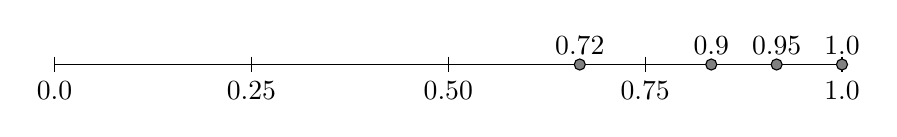
\begin{tikzpicture}
    % Draw number line
    \draw[-] (0,0) -- (10,0) node[right] {};

    % Beschriftung der Hauptmarkierungen
    \foreach \x in {0.0, 0.25, 0.50, 0.75, 1.0} {
        \draw (\x*10,0.1) -- (\x*10,-0.1) node[below] {\x};
    }

    % Die Punkte plotten
    \draw[fill=gray] (0.667*10,0) circle (2pt) node[above] {$0.72$};
    \draw[fill=gray] (0.834*10,0) circle (2pt) node[above] {$0.9$};
    \draw[fill=gray] (0.917*10,0) circle (2pt) node[above] {$0.95$};
    \draw[fill=gray] (1.000*10,0) circle (2pt) node[above] {$1.0$};
\end{tikzpicture}

        \caption{Cumulative proportions used in roulette wheel selection.}
        \label{fig:number_line}
    \end{figure}
\end{Example}

%> n-Tournament <%
\subsubsection{$n$-Tournament}
This selection technique involves repeatedly organizing \enquote{tournaments},
where a subset of the population competes, and the fittest individual is chosen
as the winner \cite{Affenzeller2009}.
The process is repeated until the desired number of individual has been
selected for reproduction. The selection process consists of the following
steps:
\begin{enumerate}
    \item   Tournament Setup: A tournament is formed by randomly selecting
            a predefined number of individuals, known as the tournament size
            $n$. These individuals are the participants of the tournament.
    \item   Winner Selection: As the individuals are provided with their cost
            values, no evaluation is needed and the selection process can
            directly proceed by selecting the winner of the tournament.
            The participant with the lowest cost is declared the winner of the
            tournament and is added to the selected set of individuals.
    \item   Repetition: The process is repeated until the desired number of
            individuals has been selected.
\end{enumerate}

%> Linear Rank <%
\subsubsection{Linear Rank}
\enquote{Rank selection is the modified form of Roulette Wheel selection.
It utilizes the ranks instead of fitness value} \cite{Katoch2021}.
These ranks correspond to the position of individuals in a population ordered
by their fitness value \cite{Affenzeller2009}.
Linear Rank selection is a variation of the general rank selection, in which
the selection probabilities are calculated based on a linear function
\cite{Affenzeller2009}.
This method provides greater control over selection pressure, ensuring a
balance between exploration and exploitation \cite{Katoch2021,Affenzeller2009}.

The key idea behind linear rank selection is to rank individuals in the
population according to their fitness (e.g., cost). The fittest individual is
assigned the highest rank, while the least fit individual is assigned the
lowest rank. Selection probabilities are then calculated based on these ranks,
rather than the fitness values, associated with the individuals.
This decoupling helps mitigate the disproportionate influence of extreme
fitness values, which can otherwise dominate the selection pressure.

The selection process consists of the following steps:
\begin{enumerate}
    \item   Rank Assignment: The list of individuals passed to the selection
            method is already sorted by the individual's cost in ascending
            order. Because of that, the rank of each individual directly
            corresponds to its index in the list (starting at $0$).

    \item   Probability Calculation: The probability of selecting an individual
            is determined by the following formula:
            \begin{equation}
                p(r) = \frac{2-s}{n} + \frac{2 \cdot (s-1) \cdot (n-r)}{n^2}
            \end{equation}

            In this formula $s$ represents the selection pressure, a parameter
            that controls how strongly the method favors higher-ranked
            individuals:
            \begin{itemize}
                \item   $s = 1$: Equal probability for all ranks (random
                        selection)
                \item   $s = 2$: Linear selection where the last rank has zero
                        probability of selection.
                \item   $s > 2$: Steeper probability decay, where individual
                        with lower ranks my have no chance of selection.
            \end{itemize}

    \item   Selection Process: Analogous to the implementation of the roulette
            wheel selection, the linear rank selection also accumulates
            the calculated probabilities iteratively, stores them into an
            array and proceeds with the selection just like the roulette
            wheel selection does.
\end{enumerate}


%%% Crossover %%%
\subsection{Crossover}
Crossover is a genetic operation that combines the genetic material of two
parent chromosomes to create offspring \cite{Beligiannis2009}. This operation
is inspired by the process of genetic recombination in biological reproduction,
where traits from both parents are passed on to their offspring
\cite{goldberg1989}.
Crossover serves as the primary mechanism for introducing new combinations of
genes into the population, enabling exploration of the solution space and
promoting diversity.

All crossover methods in this study, are designed to produce two offspring
individuals from their two parents. This ensures that the best combination of
the parents' genetic material, according to the used crossover method,
has a chance to be included in the population.

Depending on the encoding of the solutions, different crossover methods can be
applied to ensure effective recombination. The following sections describe the
crossover methods implemented in this study.

\subsubsection{Uniform Crossover}
Uniform crossover is a recombination technique where each gene in the offspring
is randomly inherited from one of the two parents with equal probability
\cite{Affenzeller2009,Katoch2021}.
This method does not impose any positional bias, making it effective for
problems where the relationship between neighboring genes is not significant.

Its implementation utilizes a random binary mask determining which genes are
swapped between the two parents \cite{Katoch2021}.
For each gene position, the algorithm flips an imaginary coin to decide whether
the gene from one or the other parent will be inherited by the corresponding
child. This process ensures that both offspring inherit a random mixture of
genetic material from their parents.

\subsubsection{$n$-Point}
This crossover technique exchanges genetic material
between two parent chromosomes at one or more crossover points. These methods
alternate segments of the genes from each parent to produce offspring
\cite{Affenzeller2009}.
$n$-Point crossover is also commonly known as single-point or multipoint
crossover, where single-point crossover is just a special case of $n$-Point
crossover with $n=1$ \cite{Affenzeller2009}.

\subsubsection{Ordered}
The ordered crossover method used primarily for problems where the order of
elements in a solution is significant (e.g. permutation encodings)
\cite{Katoch2021}.
An example for ordered crossover is shown in figure \ref{fig:ordered_crossover}.
The process involves the following steps \cite{Katoch2021}:
\begin{enumerate}
    \item   Two random indices are selected, defining a segment of genes from
            each parent. This \enquote{middle segment} will be directly copied
            into the corresponding positions of the offspring.

    \item   The remaining genes are taken from the other parent respectively,
            skipping the genes which are included in the copied over section,
            and filling the positions after middle section first.

    \item   This process is performed twice: once with the middle segment taken
            from the first parent and the remainder from the second, and
            vice versa. This produces two offspring chromosomes from the two
            parents.
\end{enumerate}

The order crossover ensures that genes maintain their original relative order
while ensuring that no duplicates exist, which is especially important for
permutation encodings like the indirect encoding in this study.

\begin{figure}[]
    \centering
    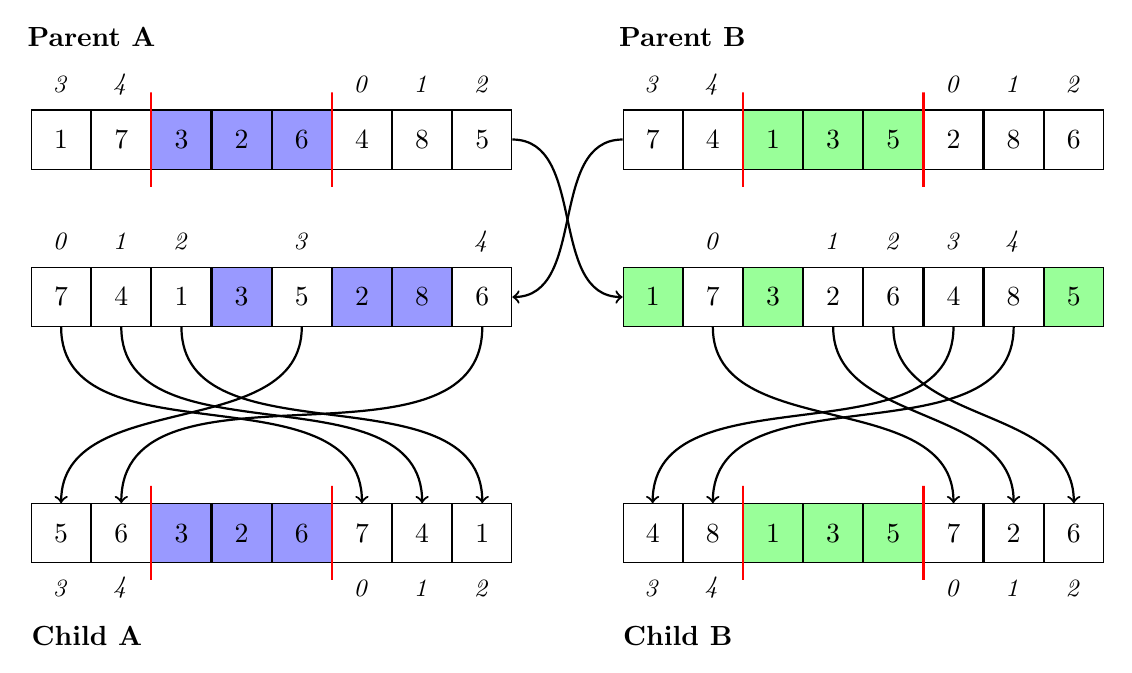
\begin{tikzpicture}
    % Define styles for the nodes
    \tikzstyle{cell} = [
        rectangle, text centered, draw,
        minimum width=0.75cm, minimum height=0.75cm
    ];

    \tikzstyle{index} = [
        text centered, font=\small, yshift=-0.3cm
    ];

    \tikzstyle{index_below} = [
        text centered, font=\small, yshift=0.3cm
    ];

    \tikzstyle{arrow} = [thick];

    % Parent A
    \node[cell]                             (a0)                {1};
    \node[cell, anchor=west]                (a1) at (a0.east)   {7};
    \node[cell, anchor=west, fill=blue!40]  (a2) at (a1.east)   {3};
    \node[cell, anchor=west, fill=blue!40]  (a3) at (a2.east)   {2};
    \node[cell, anchor=west, fill=blue!40]  (a4) at (a3.east)   {6};
    \node[cell, anchor=west]                (a5) at (a4.east)   {4};
    \node[cell, anchor=west]                (a6) at (a5.east)   {8};
    \node[cell, anchor=west]                (a7) at (a6.east)   {5};

    \node[
        anchor=west, xshift=-0.05cm, yshift=1.3cm, inner sep=0
    ] (parent_a) at (a0.west) {\textbf{Parent A}};

    \node[index, above of=a5] {\textit{0}};
    \node[index, above of=a6] {\textit{1}};
    \node[index, above of=a7] {\textit{2}};
    \node[index, above of=a0] {\textit{3}};
    \node[index, above of=a1] {\textit{4}};

    % Parent B
    \node[cell, anchor=west, xshift=1.4cm]  (b0) at (a7.east)   {7};
    \node[cell, anchor=west]                (b1) at (b0.east)   {4};
    \node[cell, anchor=west, fill=green!40] (b2) at (b1.east)   {1};
    \node[cell, anchor=west, fill=green!40] (b3) at (b2.east)   {3};
    \node[cell, anchor=west, fill=green!40] (b4) at (b3.east)   {5};
    \node[cell, anchor=west]                (b5) at (b4.east)   {2};
    \node[cell, anchor=west]                (b6) at (b5.east)   {8};
    \node[cell, anchor=west]                (b7) at (b6.east)   {6};

    \node[
        anchor=west, xshift=-0.05cm, yshift=1.3cm, inner sep=0
    ] (parent_b) at (b0.west) {\textbf{Parent B}};

    \node[index, above of=b5] {\textit{0}};
    \node[index, above of=b6] {\textit{1}};
    \node[index, above of=b7] {\textit{2}};
    \node[index, above of=b0] {\textit{3}};
    \node[index, above of=b1] {\textit{4}};


    % Cut Lines for A
    \draw[thick, red] (a1.east) -- ++(0cm,0.6cm) -- ++(0cm,-1.2cm);
    \draw[thick, red] (a4.east) -- ++(0cm,0.6cm) -- ++(0cm,-1.2cm);

    % Cut Lines for B
    \draw[thick, red] (b1.east) -- ++(0cm,0.6cm) -- ++(0cm,-1.2cm);
    \draw[thick, red] (b4.east) -- ++(0cm,0.6cm) -- ++(0cm,-1.2cm);

    % Parent B'
    \node[cell, anchor=west, yshift=-2cm]   (b'0) at (a0.west)    {7};
    \node[cell, anchor=west]                (b'1) at (b'0.east)   {4};
    \node[cell, anchor=west]                (b'2) at (b'1.east)   {1};
    \node[cell, anchor=west, fill=blue!40]  (b'3) at (b'2.east)   {3};
    \node[cell, anchor=west]                (b'4) at (b'3.east)   {5};
    \node[cell, anchor=west, fill=blue!40]  (b'5) at (b'4.east)   {2};
    \node[cell, anchor=west, fill=blue!40]  (b'6) at (b'5.east)   {8};
    \node[cell, anchor=west]                (b'7) at (b'6.east)   {6};

    \node[index, above of=b'0] {\textit{0}};
    \node[index, above of=b'1] {\textit{1}};
    \node[index, above of=b'2] {\textit{2}};
    \node[index, above of=b'4] {\textit{3}};
    \node[index, above of=b'7] {\textit{4}};

    % Parent A'
    \node[cell, anchor=west, xshift=1.4cm, fill=green!40]  (a'0) at (b'7.east)   {1};
    \node[cell, anchor=west]                (a'1) at (a'0.east)   {7};
    \node[cell, anchor=west, fill=green!40] (a'2) at (a'1.east)   {3};
    \node[cell, anchor=west]                (a'3) at (a'2.east)   {2};
    \node[cell, anchor=west]                (a'4) at (a'3.east)   {6};
    \node[cell, anchor=west]                (a'5) at (a'4.east)   {4};
    \node[cell, anchor=west]                (a'6) at (a'5.east)   {8};
    \node[cell, anchor=west, fill=green!40] (a'7) at (a'6.east)   {5};

    \node[index, above of=a'1] {\textit{0}};
    \node[index, above of=a'3] {\textit{1}};
    \node[index, above of=a'4] {\textit{2}};
    \node[index, above of=a'5] {\textit{3}};
    \node[index, above of=a'6] {\textit{4}};

    % Arrows
    \draw[->, thick, out=0, in=180] (a7.east) to (a'0.west);
    \draw[->, thick, out=180, in=0] (b0.west) to (b'7.east);

    % Child A
    \node[cell, anchor=west, yshift=-3.0cm] (ca0) at (b'0.west) {5};
    \node[cell, anchor=west]                (ca1) at (ca0.east) {6};
    \node[cell, anchor=west, fill=blue!40]  (ca2) at (ca1.east) {3};
    \node[cell, anchor=west, fill=blue!40]  (ca3) at (ca2.east) {2};
    \node[cell, anchor=west, fill=blue!40]  (ca4) at (ca3.east) {6};
    \node[cell, anchor=west]                (ca5) at (ca4.east) {7};
    \node[cell, anchor=west]                (ca6) at (ca5.east) {4};
    \node[cell, anchor=west]                (ca7) at (ca6.east) {1};

    \node[
        anchor=west, yshift=-1.3cm, inner sep=0
    ] (child_a) at (ca0.west) {\textbf{Child A}};

    \node[index_below, below of=ca5] {\textit{0}};
    \node[index_below, below of=ca6] {\textit{1}};
    \node[index_below, below of=ca7] {\textit{2}};
    \node[index_below, below of=ca0] {\textit{3}};
    \node[index_below, below of=ca1] {\textit{4}};

    % Child B
    \node[cell, anchor=west, xshift=1.4cm]  (cb0) at (ca7.east) {4};
    \node[cell, anchor=west]                (cb1) at (cb0.east) {8};
    \node[cell, anchor=west, fill=green!40] (cb2) at (cb1.east) {1};
    \node[cell, anchor=west, fill=green!40] (cb3) at (cb2.east) {3};
    \node[cell, anchor=west, fill=green!40] (cb4) at (cb3.east) {5};
    \node[cell, anchor=west]                (cb5) at (cb4.east) {7};
    \node[cell, anchor=west]                (cb6) at (cb5.east) {2};
    \node[cell, anchor=west]                (cb7) at (cb6.east) {6};

    \node[
        anchor=west, yshift=-1.3cm, inner sep=0
    ] (child_b) at (cb0.west) {\textbf{Child B}};

    \node[index_below, below of=cb5] {\textit{0}};
    \node[index_below, below of=cb6] {\textit{1}};
    \node[index_below, below of=cb7] {\textit{2}};
    \node[index_below, below of=cb0] {\textit{3}};
    \node[index_below, below of=cb1] {\textit{4}};

    % Cut Lines for Child A
    \draw[thick, red] (ca1.east) -- ++(0cm,0.6cm) -- ++(0cm,-1.2cm);
    \draw[thick, red] (ca4.east) -- ++(0cm,0.6cm) -- ++(0cm,-1.2cm);

    % Cut Lines for Child B
    \draw[thick, red] (cb1.east) -- ++(0cm,0.6cm) -- ++(0cm,-1.2cm);
    \draw[thick, red] (cb4.east) -- ++(0cm,0.6cm) -- ++(0cm,-1.2cm);


    % Children A - Arrows
    \draw[->, thick, out=270, in=90] (b'0.south) to (ca5.north);
    \draw[->, thick, out=270, in=90] (b'1.south) to (ca6.north);
    \draw[->, thick, out=270, in=90] (b'2.south) to (ca7.north);
    \draw[->, thick, out=270, in=90] (b'4.south) to (ca0.north);
    \draw[->, thick, out=270, in=90] (b'7.south) to (ca1.north);

    % Children B - Arrows
    \draw[->, thick, out=270, in=90] (a'1.south) to (cb5.north);
    \draw[->, thick, out=270, in=90] (a'3.south) to (cb6.north);
    \draw[->, thick, out=270, in=90] (a'4.south) to (cb7.north);
    \draw[->, thick, out=270, in=90] (a'5.south) to (cb0.north);
    \draw[->, thick, out=270, in=90] (a'6.south) to (cb1.north);

\end{tikzpicture}

    \caption{Ordered Crossover}
    \label{fig:ordered_crossover}
\end{figure}

\subsubsection{Partially Mapped (PMX)}
Partially Mapped Crossover (PMX) is a technique designed for
permutation-based problems.
As such, PMX ensures that the offspring inherit both positional and order
information from their parents, while preserving the validity of the
permutation \cite{Katoch2021}.

The PMX crossover algorithm initially generates two random indices, which are
used to divide each parent chromosome into three parts: a left, middle and
right one. The middle parts are transferred to the child chromosomes as is,
illustrated in figure \ref{fig:pmx_middle_part_crossover}.

\begin{figure}[]
    \centering
    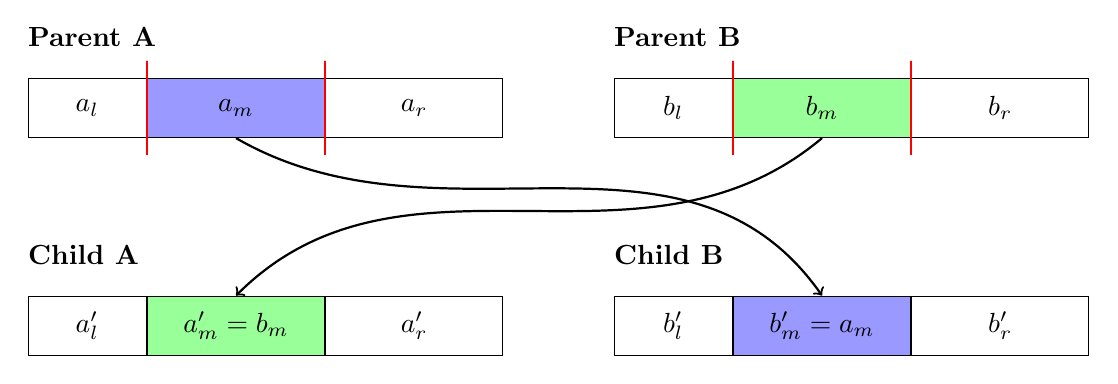
\begin{tikzpicture}
    % Define styles for the nodes
    \tikzstyle{cell_x2} = [
        text centered, draw, minimum height=0.75cm,
        minimum width=1.50cm
    ]
    \tikzstyle{cell_x3} = [
            text centered, draw, minimum height=0.75cm,
        minimum width=2.25cm
    ]

    % Parent A
    \node[cell_x2] (al) {$a_l$};
    \node[cell_x3, anchor=west, fill=blue!40] (am) at (al.east) {$a_m$};
    \node[cell_x3, anchor=west] (ar) at (am.east) {$a_r$};

    % Label for Parent A
    \node[
        anchor=west, yshift=0.9cm, inner sep=0
    ] (parent_a) at (al.west) {\textbf{Parent A}};

    % Parent B
    \node[cell_x2, anchor=west, xshift=1.4cm] (bl) at (ar.east) {$b_l$};
    \node[cell_x3, anchor=west, fill=green!40] (bm) at (bl.east) {$b_m$};
    \node[cell_x3, anchor=west] (br) at (bm.east) {$b_r$};

    \node[
        anchor=west, yshift=0.9cm, inner sep=0
    ] (parent_b) at (bl.west) {\textbf{Parent B}};

    % Cut Lines for A
    \draw[thick, red] (al.east) -- ++(0cm,0.6cm) -- ++(0cm,-1.2cm);
    \draw[thick, red] (am.east) -- ++(0cm,0.6cm) -- ++(0cm,-1.2cm);

    % Cut Lines for A
    \draw[thick, red] (bl.east) -- ++(0cm,0.6cm) -- ++(0cm,-1.2cm);
    \draw[thick, red] (bm.east) -- ++(0cm,0.6cm) -- ++(0cm,-1.2cm);


    % Child A
    \node[cell_x2, below= 2cm of al] (cal) {$a'_l$};
    \node[cell_x3, anchor=west, fill=green!40] (cam) at (cal.east) {$a'_m = b_m$};
    \node[cell_x3, anchor=west] (car) at (cam.east) {$a'_r$};

    % Label for Child A
    \node[
        anchor=west, yshift=0.9cm, inner sep=0
    ] (child_a) at (cal.west) {\textbf{Child A}};


    % Child B
    \node[cell_x2, below= 2cm of bl] (cbl) {$b'_l$};
    \node[cell_x3, anchor=west, fill=blue!40] (cbm) at (cbl.east) {$b'_m = a_m$};
    \node[cell_x3, anchor=west] (cbr) at (cbm.east) {$b'_r$};

    % Label for Child B
    \node[
        anchor=west, yshift=0.9cm, inner sep=0
    ] (child_b) at (cbl.west) {\textbf{Child B}};

    % Exchange Arrows
    \draw[->, thick, out=330, in=125] (am.south) to (cbm.north);

    \draw[->, thick, out=220, in=45] (bm.south) to (cam.north);

\end{tikzpicture}


    \caption{Illustration of exchanging fixed genes in PMX crossover.}
    \label{fig:pmx_middle_part_crossover}
\end{figure}

After exchanging the middle parts of the parent chromosomes, the goal of
the crossover operation is to preserve the order of the genes from the
respective parent chromosome as much as possible. It is not possible to simply
copy $a_l$ to $a'_l$, $a_r$ to $a'_r$ and so on, because this could introduce
duplicate genes due to the middle part of each child chromosome originating
from the respective other parent. Therefore, a mapping is introduced, which
helps to resolve these duplicates and ensures valid permutations as result of
the crossover operation. Figure \ref{fig:pmx_mapping} visualizes how the
middle parts are used to create a mapping, which is then utilized to resolve
potential gene duplications.

\begin{figure}[]
    \centering
    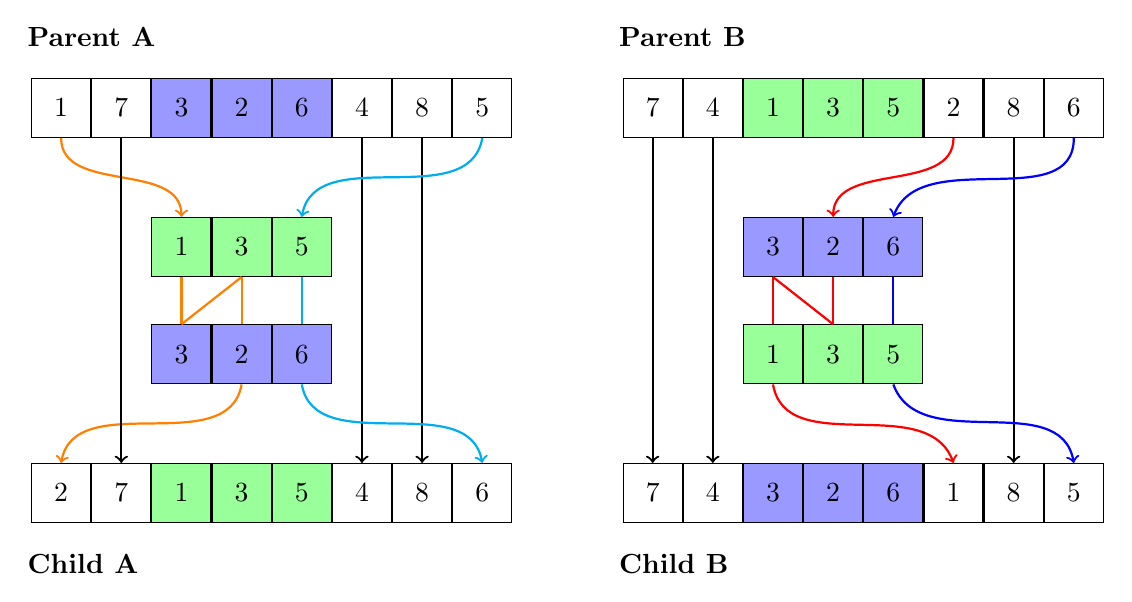
\begin{tikzpicture}
    % Define styles for the nodes
    \tikzstyle{cell} = [
        rectangle, text centered, draw,
        minimum width=0.75cm, minimum height=0.75cm
    ]

    \tikzstyle{arrow} = [thick]

    % Parent A
    \node[cell]                             (a0)                {1};
    \node[cell, anchor=west]                (a1) at (a0.east)   {7};
    \node[cell, anchor=west, fill=blue!40]  (a2) at (a1.east)   {3};
    \node[cell, anchor=west, fill=blue!40]  (a3) at (a2.east)   {2};
    \node[cell, anchor=west, fill=blue!40]  (a4) at (a3.east)   {6};
    \node[cell, anchor=west]                (a5) at (a4.east)   {4};
    \node[cell, anchor=west]                (a6) at (a5.east)   {8};
    \node[cell, anchor=west]                (a7) at (a6.east)   {5};

    \node[
        anchor=west, xshift=-0.05cm, yshift=0.9cm, inner sep=0
    ] (parent_a) at (a0.west) {\textbf{Parent A}};

    % Parent B
    \node[cell, anchor=west, xshift=1.4cm]  (b0) at (a7.east)   {7};
    \node[cell, anchor=west]                (b1) at (b0.east)   {4};
    \node[cell, anchor=west, fill=green!40] (b2) at (b1.east)   {1};
    \node[cell, anchor=west, fill=green!40] (b3) at (b2.east)   {3};
    \node[cell, anchor=west, fill=green!40] (b4) at (b3.east)   {5};
    \node[cell, anchor=west]                (b5) at (b4.east)   {2};
    \node[cell, anchor=west]                (b6) at (b5.east)   {8};
    \node[cell, anchor=west]                (b7) at (b6.east)   {6};

    \node[
        anchor=west, xshift=-0.05cm, yshift=0.9cm, inner sep=0
    ] (parent_b) at (b0.west) {\textbf{Parent B}};


    % Map B -> A
    \node[cell, below=1cm of a2, fill=green!40] (map_ba00) {1};
    \node[cell, anchor=west, fill=green!40] (map_ba01) at (map_ba00.east) {3};
    \node[cell, anchor=west, fill=green!40] (map_ba02) at (map_ba01.east) {5};

    \node[cell, below=0.6cm of map_ba00, fill=blue!40] (map_ba10) {3};
    \node[cell, anchor=west, fill=blue!40] (map_ba11) at (map_ba10.east) {2};
    \node[cell, anchor=west, fill=blue!40] (map_ba12) at (map_ba11.east) {6};

    % Map A -> B
    \node[cell, below=1cm of b2, fill=blue!40] (map_ab00) {3};
    \node[cell, anchor=west, fill=blue!40] (map_ab01) at (map_ab00.east) {2};
    \node[cell, anchor=west, fill=blue!40] (map_ab02) at (map_ab01.east) {6};

    \node[cell, below=0.6cm of map_ab00, fill=green!40] (map_ab10) {1};
    \node[cell, anchor=west, fill=green!40] (map_ab11) at (map_ab10.east) {3};
    \node[cell, anchor=west, fill=green!40] (map_ab12) at (map_ab11.east) {5};


    % Child A
    \node[cell, below=4.125cm of a0]        (ca0)               {2};
    \node[cell, anchor=west]                (ca1) at (ca0.east) {7};
    \node[cell, anchor=west, fill=green!40] (ca2) at (ca1.east) {1};
    \node[cell, anchor=west, fill=green!40] (ca3) at (ca2.east) {3};
    \node[cell, anchor=west, fill=green!40] (ca4) at (ca3.east) {5};
    \node[cell, anchor=west]                (ca5) at (ca4.east) {4};
    \node[cell, anchor=west]                (ca6) at (ca5.east) {8};
    \node[cell, anchor=west]                (ca7) at (ca6.east) {6};

    \node[
        anchor=west, xshift=-0.05cm, yshift=-0.9cm, inner sep=0
    ] (child_a) at (ca0.west) {\textbf{Child A}};

    % Child B
    \node[cell, below=4.125cm of b0]        (cb0)               {7};
    \node[cell, anchor=west]                (cb1) at (cb0.east) {4};
    \node[cell, anchor=west, fill=blue!40] (cb2) at (cb1.east) {3};
    \node[cell, anchor=west, fill=blue!40] (cb3) at (cb2.east) {2};
    \node[cell, anchor=west, fill=blue!40] (cb4) at (cb3.east) {6};
    \node[cell, anchor=west]                (cb5) at (cb4.east) {1};
    \node[cell, anchor=west]                (cb6) at (cb5.east) {8};
    \node[cell, anchor=west]                (cb7) at (cb6.east) {5};

    \node[
        anchor=west, xshift=-0.05cm, yshift=-0.9cm, inner sep=0
    ] (child_b) at (cb0.west) {\textbf{Child B}};

    % Arrows 1
    \draw[arrow, ->, orange, out=270, in=90] (a0.south) to (map_ba00.north);
    \draw[arrow, orange] (map_ba00.south) to (map_ba10.north);
    \draw[arrow, orange] (map_ba10.north) to (map_ba01.south);
    \draw[arrow, orange] (map_ba01.south) to (map_ba11.north);
    \draw[arrow, ->, orange, out=260, in=80] (map_ba11.south) to (ca0.north);

    % Arrow 2
    \draw[arrow, ->, black] (a1.south) to (ca1.north);

    % Arrow 3
    \draw[arrow, ->, black] (a5.south) to (ca5.north);

    % Arrow 4
    \draw[arrow, ->, black] (a6.south) to (ca6.north);

    % Arrow 5
    \draw[arrow, ->, cyan, out=260, in=80] (a7.south) to (map_ba02.north);
    \draw[arrow, cyan] (map_ba02.south) to (map_ba12.north);
    \draw[arrow, ->, cyan, out=280, in=100] (map_ba12.south) to (ca7.north);


    % Arrow 6
    \draw[arrow, ->] (b0.south) to (cb0.north);

    % Arrow 7
    \draw[arrow, ->] (b1.south) to (cb1.north);

    % Arrow 8
    \draw[arrow, ->, red, out=270, in=90] (b5.south) to (map_ab01.north);
    \draw[arrow, red] (map_ab01.south) to (map_ab11.north);
    \draw[arrow, red] (map_ab11.north) to (map_ab00.south);
    \draw[arrow, red] (map_ab00.south) to (map_ab10.north);
    \draw[arrow, ->, red, out=280, in=110] (map_ab10.south) to (cb5.north);

    % Arrow 9
    \draw[arrow, ->] (b6.south) to (cb6.north);

    % Arrow 10
    \draw[arrow, ->, blue, out=270, in=70] (b7.south) to (map_ab02.north);
    \draw[arrow, blue] (map_ab02.south) to (map_ab12.north);
    \draw[arrow, ->, blue, out=290, in=100] (map_ab12.south) to (cb7.north);

\end{tikzpicture}


    \caption{Visualization of gene mapping in PMX crossover.}
    \label{fig:pmx_mapping}
\end{figure}

\subsubsection{$n$-Trade}
\label{n-trade crossover}
The n-Trade crossover is a recombination technique specifically developed
for the direct encoding in this study. It facilitates the exchange of time slot
allocations between two events while preserving the total number of allocated
time slots per event. This ensures that the \textit{AssignTimeConstraint}
remains satisfied, which is a critical requirement of the direct encoding and
an inherent component of the direct encoded algorithm's design.

The crossover method is based on a \textit{trade} operation, which is performed
for pairs of time allocations. As the $n$-Trade crossover is exclusively used
in the direct encoding, this means, that trades are performed between the
time allocations (represented by bit vectors) of events. Therefore, this
crossover method iterates the genes of the two parent chromosomes
simultaneously, yielding pairs of such bit vectors. These bit vectors always
represent time allocations for the \textit{same} event. For each of those pairs
of bit vectors the following trade algorithm is performed.

First, all bits set in one bit vector and not set in the other one are
determined (for both bit vectors). The resulting bit vectors form the pool of
time allocations, each of the original time allocations can potentially trade
for another one. For each trade both bit vectors randomly select
one of their tradable bits, hand it over to the other bit vector and receive
another bit in return. Example \ref{ex:n-trade-crossover} visualizes such a
trade operation.

By carefully selecting only the time slots not currently allocated to the trade
partner, this method guarantees that the total number of time slots allocated
to each event remains unchanged.
The parameter $n$ controls the number of trades performed during the crossover
operations. When $n=1$, the crossover executes a single trade between the two
events, resulting in minimal recombination. For larger values of $n$, multiple
trades occur, increasing the diversity introduced in the offspring chromosomes.

The design of this crossover operator was inspired by the local search moves
used in the simulated annealing algorithm described in \cite{demiroBitvec},
which originate from \cite{Fonseca2014}.

\begin{minipage}{\textwidth}
    \begin{Example}[$n$-Trade crossover with $n=2$]
        \begin{minipage}{\textwidth}
            \centering
            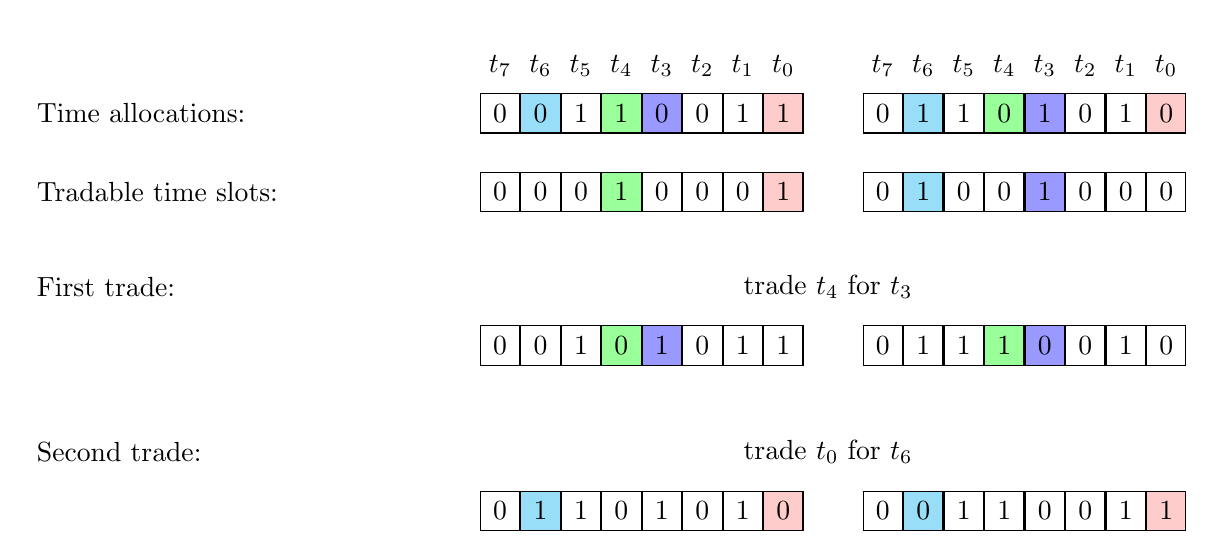
\begin{tikzpicture}
    \tikzstyle{cell} = [
        rectangle, text centered, draw,
        minimum width=0.5cm, minimum height=0.5cm
    ]

    \tikzstyle{label} = [text centered, yshift=-0.4cm]

    \tikzstyle{desc} = [align=left, text width=5cm]

    \tikzstyle{trade_desc} = [
        anchor=west, xshift=0.5cm, align=center, minimum width=8.95cm
    ]

    \node (top_spacer) [] {};

    % Text column
    \node[desc, below=0.6cm of top_spacer] (time_alloc) {Time allocations:};
    \node[desc, below of=time_alloc] (tradable) {Tradable time slots:};
    \node[desc, below of=tradable, yshift=-0.2cm] (1st_trade) {First trade:};
    \node[desc, below of=1st_trade, yshift=-1.1cm] (2nd_trade) {Second trade:};

    % Time allocation 1
    \node[cell, anchor=west, xshift=0.5cm] (a7) at (time_alloc.east) {0};
    \node[cell, anchor=west, fill=cyan!40] (a6) at (a7.east) {0};
    \node[cell, anchor=west] (a5) at (a6.east) {1};
    \node[cell, anchor=west, fill=green!40] (a4) at (a5.east) {1};
    \node[cell, anchor=west, fill=blue!40] (a3) at (a4.east) {0};
    \node[cell, anchor=west] (a2) at (a3.east) {0};
    \node[cell, anchor=west] (a1) at (a2.east) {1};
    \node[cell, anchor=west, fill=pink!80] (a0) at (a1.east) {1};

    \node[label, above of=a7] (tia7) {$t_7$};
    \node[label, above of=a6] (tia6) {$t_6$};
    \node[label, above of=a5] (tia5) {$t_5$};
    \node[label, above of=a4] (tia4) {$t_4$};
    \node[label, above of=a3] (tia3) {$t_3$};
    \node[label, above of=a2] (tia2) {$t_2$};
    \node[label, above of=a1] (tia1) {$t_1$};
    \node[label, above of=a0] (tia0) {$t_0$};


    % Time allocation 2
    \node[cell, anchor=west, xshift=0.75cm] (b7) at (a0.east) {0};
    \node[cell, anchor=west, fill=cyan!40] (b6) at (b7.east) {1};
    \node[cell, anchor=west] (b5) at (b6.east) {1};
    \node[cell, anchor=west, fill=green!40] (b4) at (b5.east) {0};
    \node[cell, anchor=west, fill=blue!40] (b3) at (b4.east) {1};
    \node[cell, anchor=west] (b2) at (b3.east) {0};
    \node[cell, anchor=west] (b1) at (b2.east) {1};
    \node[cell, anchor=west, fill=pink!80] (b0) at (b1.east) {0};

    \node[label, above of=b7] (tib7) {$t_7$};
    \node[label, above of=b6] (tib6) {$t_6$};
    \node[label, above of=b5] (tib5) {$t_5$};
    \node[label, above of=b4] (tib4) {$t_4$};
    \node[label, above of=b3] (tib3) {$t_3$};
    \node[label, above of=b2] (tib2) {$t_2$};
    \node[label, above of=b1] (tib1) {$t_1$};
    \node[label, above of=b0] (tib0) {$t_0$};


    % Tradable time slots 1
    \node[cell, anchor=west, xshift=0.5cm] (ta7) at (tradable.east) {0};
    \node[cell, anchor=west] (ta6) at (ta7.east) {0};
    \node[cell, anchor=west] (ta5) at (ta6.east) {0};
    \node[cell, anchor=west, fill=green!40] (ta4) at (ta5.east) {1};
    \node[cell, anchor=west] (ta3) at (ta4.east) {0};
    \node[cell, anchor=west] (ta2) at (ta3.east) {0};
    \node[cell, anchor=west] (ta1) at (ta2.east) {0};
    \node[cell, anchor=west, fill=pink!80] (ta0) at (ta1.east) {1};

    % Tradable time slots 2
    \node[cell, anchor=west, xshift=0.75cm] (tb7) at (ta0.east) {0};
    \node[cell, anchor=west, fill=cyan!40] (tb6) at (tb7.east) {1};
    \node[cell, anchor=west] (tb5) at (tb6.east) {0};
    \node[cell, anchor=west] (tb4) at (tb5.east) {0};
    \node[cell, anchor=west, fill=blue!40] (tb3) at (tb4.east) {1};
    \node[cell, anchor=west] (tb2) at (tb3.east) {0};
    \node[cell, anchor=west] (tb1) at (tb2.east) {0};
    \node[cell, anchor=west] (ta0) at (tb1.east) {0};

    % 1st trade
    \node[trade_desc] (1st_trade_desc) at (1st_trade.east) {
        trade $t_4$ for $t_3$
    };

    % Time allocation 1'
    \node[cell, anchor=west, yshift=-0.75cm] (a7') at (1st_trade_desc.west) {0};
    \node[cell, anchor=west] (a6') at (a7'.east) {0};
    \node[cell, anchor=west] (a5') at (a6'.east) {1};
    \node[cell, anchor=west, fill=green!40] (a4') at (a5'.east) {0};
    \node[cell, anchor=west, fill=blue!40] (a3') at (a4'.east) {1};
    \node[cell, anchor=west] (a2') at (a3'.east) {0};
    \node[cell, anchor=west] (a1') at (a2'.east) {1};
    \node[cell, anchor=west] (a0') at (a1'.east) {1};

    % Time allocation 2'
    \node[cell, anchor=west, xshift=0.75cm] (b7') at (a0'.east) {0};
    \node[cell, anchor=west] (b6') at (b7'.east) {1};
    \node[cell, anchor=west] (b5') at (b6'.east) {1};
    \node[cell, anchor=west, fill=green!40] (b4') at (b5'.east) {1};
    \node[cell, anchor=west, fill=blue!40] (b3') at (b4'.east) {0};
    \node[cell, anchor=west] (b2') at (b3'.east) {0};
    \node[cell, anchor=west] (b1') at (b2'.east) {1};
    \node[cell, anchor=west] (b0') at (b1'.east) {0};


    % 2nd trade
    \node[trade_desc] (2nd_trade_desc) at (2nd_trade.east) {
        trade $t_0$ for $t_6$
    };

    % Time allocation 1''
    \node[cell, anchor=west, yshift=-0.75cm] (a7'') at (2nd_trade_desc.west) {0};
    \node[cell, anchor=west, fill=cyan!40] (a6'') at (a7''.east) {1};
    \node[cell, anchor=west] (a5'') at (a6''.east) {1};
    \node[cell, anchor=west] (a4'') at (a5''.east) {0};
    \node[cell, anchor=west] (a3'') at (a4''.east) {1};
    \node[cell, anchor=west] (a2'') at (a3''.east) {0};
    \node[cell, anchor=west] (a1'') at (a2''.east) {1};
    \node[cell, anchor=west, fill=pink!80] (a0'') at (a1''.east) {0};

    % Time allocation 2''
    \node[cell, anchor=west, xshift=0.75cm] (b7'') at (a0''.east) {0};
    \node[cell, anchor=west, fill=cyan!40] (b6'') at (b7''.east) {0};
    \node[cell, anchor=west] (b5'') at (b6''.east) {1};
    \node[cell, anchor=west] (b4'') at (b5''.east) {1};
    \node[cell, anchor=west] (b3'') at (b4''.east) {0};
    \node[cell, anchor=west] (b2'') at (b3''.east) {0};
    \node[cell, anchor=west] (b1'') at (b2''.east) {1};
    \node[cell, anchor=west, fill=pink!80] (b0'') at (b1''.east) {1};

\end{tikzpicture}
            \label{ex:n-trade-crossover}
        \end{minipage}
    \end{Example}
\end{minipage}

\subsection{Mutation}
Mutation methods play a critical role in maintaining diversity within the
population by introducing random changes to individual solutions
\cite{Katoch2021,Affenzeller2009}.
In this study, the mutation methods have mostly been tailored to specific
characteristics of the direct or indirect encoding scheme.
This encoding-specific design ensures that the mutations not only introduce
meaningful variations but also respect the structural and constraint
requirements of the respective encodings.
For the direct encoding, the methods focus on modifying time slot allocations
while maintaining constraint feasibility, whereas for the direct encoding, they
ensure introducing meaningful variation into the event sequencing logic, without
breaking the permutation encoding.

\subsubsection{Swap}
The swap mutation method is the only mutation operator that the framework
(see \ref{Generic Framework for Genetic Algorithms}) provides a prebuilt
implementation for.
Its generic nature makes it encoding-independent, allowing it to perform simple
yet effective modifications to a chromosome without being tailored to any
specific representation.

In the swap mutation, the algorithm iterates over the genes of a chromosome
and swaps the currently visited gene with another randomly selected gene
from the same chromosome. However, this operation is not performed for every
gene. Instead, the mutation rate parameter determines the likelihood of a
swap occurring at each iteration. For each gene, a random number is generated,
and the swap is executed only if the number falls within the range specified
by the mutation rate.

To enhance flexibility, the swap mutation allows for two approaches of
selecting the swap position:
\begin{enumerate}
    \item   Uniform Distribution: The swap position is selected randomly across
            the entire chromosome, ensuring an even chance for all genes to
            be selected for swaps.
    \item   Favoring Neighboring Genes: By employing a normal distribution
            to generate swap positions, the algorithm biases the swaps toward
            neighboring genes, preserving localized structures within the
            chromosome while still introducing variation.
\end{enumerate}

In both cases, the implementation ensures that the generated swap position
never coincides with the index of the currently visited gene, avoiding
self-swapping and preserving the integrity of the mutation operation.

\subsubsection{Trade}
The trade mutation method is inspired by the trade crossover operation 
(see \ref{n-trade crossover}) but as it is a mutation operation, it is designed
to operate within a single chromosome rather than between two parent
chromosomes. This mutation introduces variation by performing trades between
two genes of the same chromosome.
It therefore works exactly like the $n$-Trade crossover operation
(visualized in figure \ref{ex:n-trade-crossover}), with the only difference,
that for the mutation method the time allocation bit vectors between which the
trade is performed are two genes which originate from same chromosome
(namely the chromosome which is being mutated).
In contrast, in case of the crossover method, the time allocation bit vectors
are genes from different chromosomes.

Just like other mutation operators, the trade mutation also iterates over
all genes of the given chromosome and pairs it up with another, randomly chosen
gene in the chromosome. This process is controlled by a mutation rate parameter,
which determines the likelihood of a trade being performed for each gene.

To enhance flexibility, two variants of the trade mutation are implemented:
\begin{enumerate}
    \item   Uniform Distribution: The trade partner (gene) is selected randomly
            across the entire chromosome, ensuring that all positions have an
            equal chance of being chosen.
    \item   Non-uniform Distribution: A normal distribution is employed to bias
            the selection of trade partners towards neighboring genes,
            preserving localized structures while still introducing meaningful
            variation.
\end{enumerate}

This mutation method is specifically tailored towards the direct encoding scheme
ensuring that the feasibility of the chromosome is preserved by maintaining the
total time slots allocated to each event.

\subsubsection{MoveSingleTimeAllocation}
\label{MoveSingleTimeAllocation}
The \textit{MoveSingleTimeAllocation} mutation is another operation
specifically tailored to the direct encoding used in this study. It introduces
variation by reallocating a single time slot to a new, previously unallocated
time slot, ensuring that the total number of allocated time slots remains
consistent for each event. This constraint preservation is crucial to
maintaining compliance with the \textit{AssignTimeConstraint}, which is a
fundamental aspect of the direct encoding.

This mutation operates on the chromosome, which is represented as a series of
bit vectors which encode the time slot allocations for individual events.
During the mutation, each gene in the chromosome is visited sequentially.
For each gene, a random number is generated to determine whether the mutation
should occur, based on the targeted mutation rate. If the mutation should
occur, one time slot currently allocated to the event is selected randomly
from the set bits of the bit vector. Similarly, an unallocated time slot is
chosen randomly from the unset bits. These two time slots are then swapped
by flipping their respective bits in the bit vector, effectively moving the
allocation without altering the total number of allocated time slots.
Listing \ref{code:move_single_time_alloc} includes a simplified version of
the source code for this mutation method.

\begin{lstlisting}[
    float,
    % floatplacement=H,
    language=Rust,
    caption={
        Simplified implementation of the \textit{MoveSingleTimeAllocation}
        mutation method.
    },
    label={code:move_single_time_alloc}
]
/// This function does not have a return value, because it mutates
/// the `chromosome` parameter.
fn move_single_time_alloc(
    chromosome: &mut [Bits32],
    mutation_rate: f32
) {
    for time_alloc in chromosome {
        if rand() > mutation_rate { continue; }
        // Choose a currently allocated time slot for moving.
        let selection = time_alloc
            .ones()                 // Get indices of set bits.
            .choose();              // Randomly choose an index.

        // Choose a target time slot.
        let target = time_alloc
            .zeros()                // Get indices of unset bits.
            .choose();              // Randomly choose an index.

        // Mutate the time allocation
        time_alloc.unset(selection);
        time_alloc.set(target);
    }
}
\end{lstlisting}

As with the other mutation methods developed in this study, this mutation
includes two variants. The first variant uses a uniform distribution to select
the target index, ensuring that all free time slots have an equal probability
of being chosen. The second variant introduces a normal distribution, which
biases the selection process towards nearby time slots, favoring localized
adjustments while still allowing for meaningful diversity. The differences
in selection probabilities are visualized in figure
\ref{fig:move_single_time_alloc}.

By preventing collisions that would lead to the loss of allocated time slots,
this mutation method ensures that the \textit{AssignTimeConstraint} is always
respected.

\begin{figure}
    \centering
    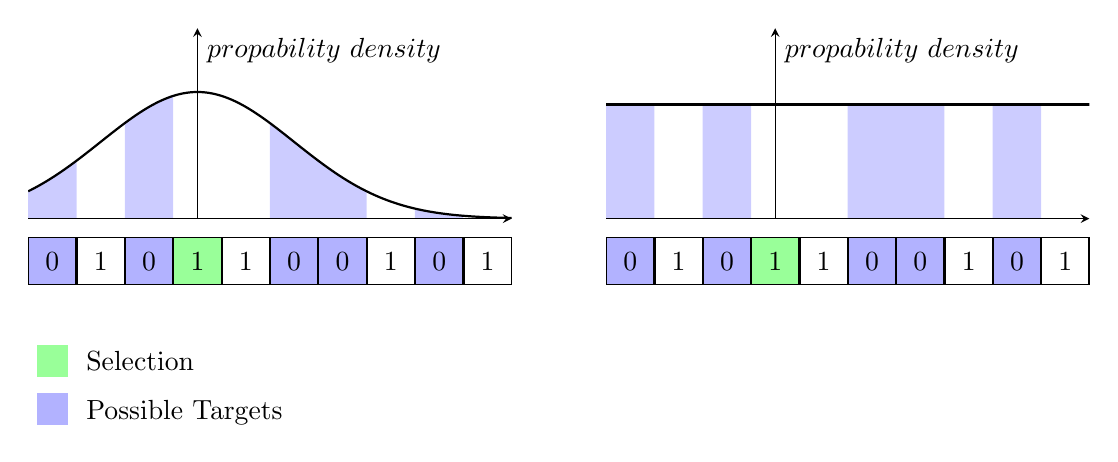
\begin{tikzpicture}
    % Plot bellcurve
    \begin{axis}[
        name=bellcurve_plot,
        axis lines=middle,
        xlabel={}, % $gene$},
        ylabel={$propability$ $density$},
        xtick=\empty,
        ytick=\empty,
        domain=-3.5:6.5,
        xmin=-3.5,
        xmax=6.5,
        ymin=0.0,
        ymax=0.3,
        % xscale=2,
        samples=1000,
        width=7.72cm,
        height=4cm,
        axis on top % ensures that the axis are rendered on top
        % smooth,
    ]
        % Bell curve
        \addplot[
            name path=bellcurve,
            black, thick
        % ] {exp(-0.5 * x^2) / sqrt(2 * pi)};
        ] {exp(-0.5 * (x/2)^2) / (2 * sqrt(2 * pi))};

        % Define the x-axis
        \addplot[
            name path=xaxis,
            draw=none
        ] coordinates {(-3.5,0) (6.5,0)};

        % Fill the area between bell curve and x-axis
        \addplot[blue!20] fill between[
            of=bellcurve and xaxis,
            soft clip={domain=-3.5:-2.5}
        ];
        \addplot[blue!20] fill between[
            of=bellcurve and xaxis,
            soft clip={domain=-1.5:-0.5}
        ];

        \addplot[blue!20] fill between[
            of=bellcurve and xaxis,
            soft clip={domain=1.5:3.5}
        ];

        \addplot[blue!20] fill between[
            of=bellcurve and xaxis,
            soft clip={domain=4.5:5.5}
        ];

    \end{axis}

    % Plot constant
    \begin{axis}[
        name=constant_plot,
        at={(bellcurve_plot.east)},
        anchor=west,
        xshift=1.2cm,
        axis lines=middle,
        xlabel={}, % $gene$},
        ylabel={$propability$ $density$},
        xtick=\empty,
        ytick=\empty,
        domain=-3.5:6.5,
        xmin=-3.5,
        xmax=6.5,
        ymin=0.0,
        ymax=0.3,
        % xscale=2,
        samples=1000,
        width=7.72cm,
        height=4cm,
        axis on top % ensures that the axis are rendered on top
        % smooth,
    ]
        % Constant
        \addplot[name path=constant, black, thick] {0.18};

        % Define the x-axis
        \addplot[
            name path=xaxis,
            draw=none
        ] coordinates {(-3.5,0) (6.5,0)};

        % Fill the area between bell curve and x-axis
        \addplot[blue!20] fill between[
            of=constant and xaxis,
            soft clip={domain=-3.5:-2.5}
        ];
        \addplot[blue!20] fill between[
            of=constant and xaxis,
            soft clip={domain=-1.5:-0.5}
        ];

        \addplot[blue!20] fill between[
            of=constant and xaxis,
            soft clip={domain=1.5:3.5}
        ];

        \addplot[blue!20] fill between[
            of=constant and xaxis,
            soft clip={domain=4.5:5.5}
        ];

    \end{axis}

    % Plot bit vectors
    \tikzstyle{cell} = [
        rectangle, text centered, draw,
        minimum width=0.6cm, minimum height=0.6cm
    ]

    % Left bit vector
    \node (n0) [
        cell, right=0 of bellcurve_plot.west, yshift=-1.75cm, fill=blue!30
    ] {0};
    \node (n1) [cell, right=0 of n0]                        {1};
    \node (n2) [cell, right=0 of n1, fill=blue!30]          {0};
    \node (n3) [cell, right=0 of n2, fill=green!40]         {1}; % "middle"
    \node (n4) [cell, right=0 of n3]                        {1};
    \node (n5) [cell, right=0 of n4, fill=blue!30]          {0};
    \node (n6) [cell, right=0 of n5, fill=blue!30]          {0};
    \node (n7) [cell, right=0 of n6]                        {1};
    \node (n8) [cell, right=0 of n7, fill=blue!30]          {0};
    \node (n9) [cell, right=0 of n8]                        {1};

    \tikzstyle{legend} = [
        rectangle, minimum width=0.4cm, minimum height=0.4cm
    ]

    \node(l0_color) [legend, fill=green!40, below=0.75cm of n0] {};
    \node(l0_text)  [right=0.1cm of l0_color] {Selection};

    \node(l1_color) [legend, fill=blue!30, below=0.2cm of l0_color] {};
    \node(l1_text)  [right=0.1cm of l1_color, yshift=-0.04cm] {Possible Targets};

    % Right bit vector
    \node (m0) [
        cell, right=0 of constant_plot.west, xshift=1.2cm, yshift=-1.75cm, fill=blue!30
    ] {0};
    \node (m1) [cell, right=0 of m0]                        {1};
    \node (m2) [cell, right=0 of m1, fill=blue!30]          {0};
    \node (m3) [cell, right=0 of m2, fill=green!40]         {1}; % "middle"
    \node (m4) [cell, right=0 of m3]                        {1};
    \node (m5) [cell, right=0 of m4, fill=blue!30]          {0};
    \node (m6) [cell, right=0 of m5, fill=blue!30]          {0};
    \node (m7) [cell, right=0 of m6]                        {1};
    \node (m8) [cell, right=0 of m7, fill=blue!30]          {0};
    \node (m9) [cell, right=0 of m8]                        {1};

\end{tikzpicture}
    \caption{
        Different selection probabilities \textit{MoveSingleTimeAllocation}
        versions: normal distribution (\textit{left}), uniform distribution
        (\textit{right})
    }
    \label{fig:move_single_time_alloc}
\end{figure}

\subsubsection{MoveSubEvent}
The \textit{MoveSubEvent} mutation builds on the principles of the
\textit{MoveSingleTimeAllocation} mutation, but operates on a group of contiguous
time slots, referred to as a \enquote{sub event}, rather than a single time
slot. This mutation relocates an entire block of continuous set bits within
the bit vector to a new position, ensuring that the total number of allocated
time slots remains unchanged and that the \textit{AssignTimeConstraint} is
preserved.

As with the \textit{MoveSingleTimeAllocation} mutation, this mutation iterates
through the genes of the chromosome, represented as bit vectors. Each bit vector
encodes the time slot allocation for a specific event. When the mutation
is triggered for a gene, based on the mutation rate, the algorithm identifies
all groups of contiguous set bits in the bit vector. These groups represent
sub events. Once a sub event is randomly selected for relocation, the algorithm
identifies valid positions in the bit vector where the entire group can fit
without causing collisions with existing allocations. A new position out of the
ones, where the sub event fits, is then chosen randomly, and the sub event is
moved by clearing the original bits and setting the bits at the new position.
A simplified version of this mutation method's implementation is shown in
listing \ref{code:move_sub_event}.

The \textit{MoveSubEvent} mutation is more computationally intensive compared
to the \textit{MoveSingleTimeAllocation} operation, as it involves identifying
all possible groups of set bits and ensuring that the selected group can be
moved without violating constraints. To address this complexity, the custom
bit vector implementation used in this study provides the specialized methods
\lstinline[language=rust]|blocks()| and \lstinline[language=rust]|holes()|
for efficiently handling these operations. These methods simplify the
development of the mutation operation and ensure good runtime performance
despite the added complexity. Example \ref{ex:move_sub_event_blocks}
illustrates the return values of these two methods based on a given
bit vector. They both return a list of bit vectors, where each bit vector
represents the \textit{start indices} of blocks of set/unset bits with a
duration which corresponds to this bit vectors index in the result list.

\begin{lstlisting}[
    float,
    % floatplacement=H,
    language=Rust,
    caption={
        Simplified implementation of the \textit{MoveSubEvent} mutation method.
    },
    label={code:move_sub_event}
]
fn move_sub_event(
    chromosome: &mut Vec<Bits32>,
    mutation_rate: f32,
) {
    for time_alloc in chromosome {
        if rand() > rate { continue; }

        // Select random sub event duration
        let (duration, block) = bits
            .blocks()                       // Get sub events.
            .enumerate()                    // Iterate with index.
            .filter(|(_, b)| !b.is_zero())  // Remove empty blocks.
            .choose(rng);                   // Randomly chose
                                            // duration.
        // Select random event (index)
        let index = block.ones().choose(rng);

        // Remove the sub event from the time allocation
        bits.unset_block(index, dduration);

        // Get all starting indices of `0`-blocks of length `d`.
        let new_index = bits.holes(duration).choose(rng);

        // Set the new block
        bits.set_block(new_index, duration);
    }
}
\end{lstlisting}

\begin{minipage}{\textwidth}
    \begin{Example}[
        Return values of the \texttt{blocks()} and \texttt{holes()} methods
    ]
        \begin{minipage}{\textwidth}
            \centering
            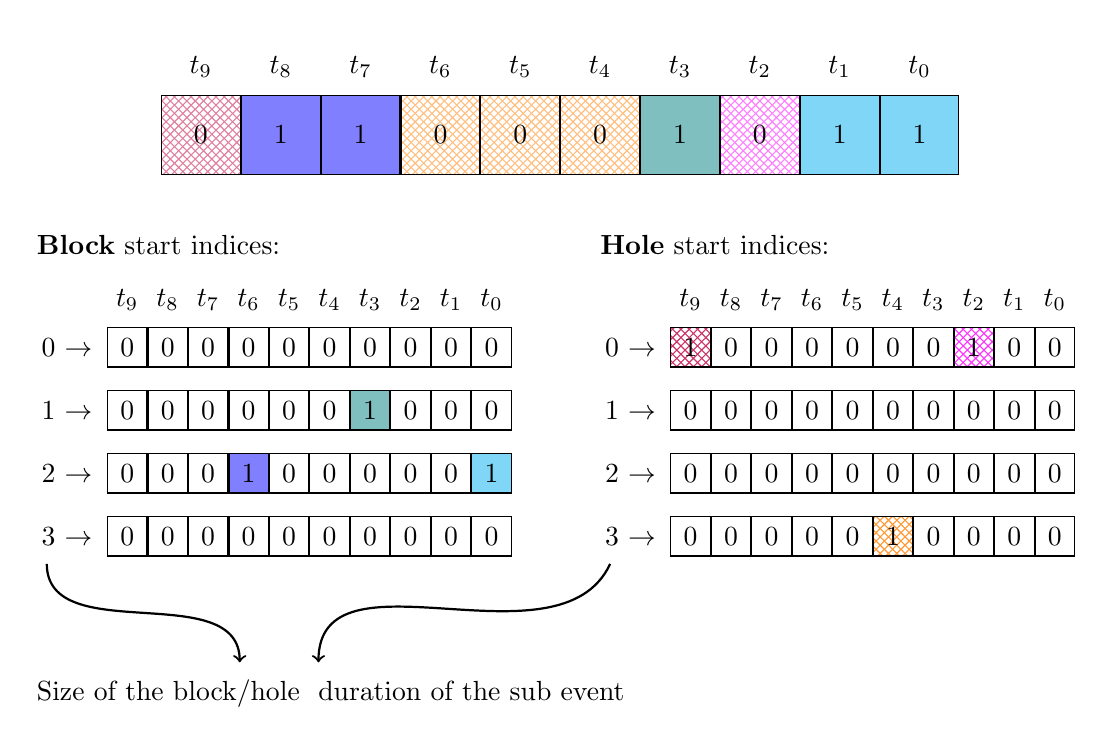
\begin{tikzpicture}
    % Define styles for the nodes
    \tikzstyle{cell} = [
        text centered, draw,
        minimum height=1cm,
        minimum width=1cm
    ]
    \tikzstyle{index} = [
        text centered,
        minimum height=1cm,
        minimum width=1cm,
        yshift=-0.14cm
    ]

    \tikzstyle{block_index} = [
        text centered,
        align=left,
        minimum height=0.5cm,
        minimum width=1cm,
        % text width=1cm,
    ]

    \tikzstyle{cell_sm} = [
        text centered, draw,
        minimum height=0.5cm,
        minimum width=0.5cm
    ]

    \tikzstyle{index_sm} = [
        text centered,
        minimum height=0.5cm,
        minimum width=0.5cm,
        yshift=-0.4cm
    ]

    \node (x0)
        [cell, pattern color=purple!50, pattern=crosshatch]
        {0};

    \node (x1)
        [cell, right=0 of x0, fill=blue!50]
        {1};

    \node (x2)
        [cell, right=0 of x1, fill=blue!50]
        {1};

    \node (x3)
        [cell, right=0 of x2, pattern color=orange!50, pattern=crosshatch]
        {0};

    \node (x4)
        [cell, right=0 of x3, pattern color=orange!50, pattern=crosshatch]
        {0};

    \node (x5)
        [cell, right=0 of x4, pattern color=orange!50, pattern=crosshatch]
        {0};

    \node (x6)
        [cell, right=0 of x5, fill=teal!50]
        {1};

    \node (x7)
        [cell, right=0 of x6, pattern color=magenta!50, pattern=crosshatch]
        {0};

    \node (x8)
        [cell, right=0 of x7, fill=cyan!50]
        {1};

    \node (x9)
        [cell, right=0 of x8, fill=cyan!50]
        {1};

    \node [index, above of=x0] {$t_9$};
    \node [index, above of=x1] {$t_8$};
    \node [index, above of=x2] {$t_7$};
    \node [index, above of=x3] {$t_6$};
    \node [index, above of=x4] {$t_5$};
    \node [index, above of=x5] {$t_4$};
    \node [index, above of=x6] {$t_3$};
    \node [index, above of=x7] {$t_2$};
    \node [index, above of=x8] {$t_1$};
    \node [index, above of=x9] {$t_0$};


    % BLOCKS %%%%%%%%%%%%%%%%%%%%%%%%%%%%%%%%%%%%%%%%%%%%%%%%%%%%%%%%%%%%%%%%%%%
    \node (block_i0)
        [block_index, below of=x0, yshift=-1.7cm, xshift=-1.7cm]
        {0 $\rightarrow$};
    \node (block_0_9) [cell_sm, right=0 of block_i0]    {0};
    \node (block_0_8) [cell_sm, right=0 of block_0_9]   {0};
    \node (block_0_7) [cell_sm, right=0 of block_0_8]   {0};
    \node (block_0_6) [cell_sm, right=0 of block_0_7]   {0};
    \node (block_0_5) [cell_sm, right=0 of block_0_6]   {0};
    \node (block_0_4) [cell_sm, right=0 of block_0_5]   {0};
    \node (block_0_3) [cell_sm, right=0 of block_0_4]   {0};
    \node (block_0_2) [cell_sm, right=0 of block_0_3]   {0};
    \node (block_0_1) [cell_sm, right=0 of block_0_2]   {0};
    \node (block_0_0) [cell_sm, right=0 of block_0_1]   {0};

    \node [above=1.3cm of block_i0.west, anchor=west] {\textbf{Block} start indices:};

    \node [index_sm, above of=block_0_9] {$t_9$};
    \node [index_sm, above of=block_0_8] {$t_8$};
    \node [index_sm, above of=block_0_7] {$t_7$};
    \node [index_sm, above of=block_0_6] {$t_6$};
    \node [index_sm, above of=block_0_5] {$t_5$};
    \node [index_sm, above of=block_0_4] {$t_4$};
    \node [index_sm, above of=block_0_3] {$t_3$};
    \node [index_sm, above of=block_0_2] {$t_2$};
    \node [index_sm, above of=block_0_1] {$t_1$};
    \node [index_sm, above of=block_0_0] {$t_0$};

    \node (block_i1)
        [block_index, below of=block_i0, yshift=0.2cm]
        {1 $\rightarrow$};
    \node (block_1_9) [cell_sm, right=0 of block_i1]    {0};
    \node (block_1_8) [cell_sm, right=0 of block_1_9]   {0};
    \node (block_1_7) [cell_sm, right=0 of block_1_8]   {0};
    \node (block_1_6) [cell_sm, right=0 of block_1_7]   {0};
    \node (block_1_5) [cell_sm, right=0 of block_1_6]   {0};
    \node (block_1_4) [cell_sm, right=0 of block_1_5]   {0};
    \node (block_1_3) [cell_sm, right=0 of block_1_4, fill=teal!50] {1};
    \node (block_1_2) [cell_sm, right=0 of block_1_3]   {0};
    \node (block_1_1) [cell_sm, right=0 of block_1_2]   {0};
    \node (block_1_0) [cell_sm, right=0 of block_1_1]   {0};

    \node (block_i2)
        [block_index, below of=block_i1, yshift=0.2cm]
        {2 $\rightarrow$};
    \node (block_2_9) [cell_sm, right=0 of block_i2]    {0};
    \node (block_2_8) [cell_sm, right=0 of block_2_9]   {0};
    \node (block_2_7) [cell_sm, right=0 of block_2_8]   {0};
    \node (block_2_6) [cell_sm, right=0 of block_2_7, fill=blue!50] {1};
    \node (block_2_5) [cell_sm, right=0 of block_2_6]   {0};
    \node (block_2_4) [cell_sm, right=0 of block_2_5]   {0};
    \node (block_2_3) [cell_sm, right=0 of block_2_4]   {0};
    \node (block_2_2) [cell_sm, right=0 of block_2_3]   {0};
    \node (block_2_1) [cell_sm, right=0 of block_2_2]   {0};
    \node (block_2_0) [cell_sm, right=0 of block_2_1, fill=cyan!50] {1};

    \node (block_i3)
        [block_index, below of=block_i2, yshift=0.2cm]
        {3 $\rightarrow$};
    \node (block_3_9) [cell_sm, right=0 of block_i3]    {0};
    \node (block_3_8) [cell_sm, right=0 of block_3_9]   {0};
    \node (block_3_7) [cell_sm, right=0 of block_3_8]   {0};
    \node (block_3_6) [cell_sm, right=0 of block_3_7]   {0};
    \node (block_3_5) [cell_sm, right=0 of block_3_6]   {0};
    \node (block_3_4) [cell_sm, right=0 of block_3_5]   {0};
    \node (block_3_3) [cell_sm, right=0 of block_3_4]   {0};
    \node (block_3_2) [cell_sm, right=0 of block_3_3]   {0};
    \node (block_3_1) [cell_sm, right=0 of block_3_2]   {0};
    \node (block_3_0) [cell_sm, right=0 of block_3_1]   {0};


    % HOLES %%%%%%%%%%%%%%%%%%%%%%%%%%%%%%%%%%%%%%%%%%%%%%%%%%%%%%%%%%%%%%%%%%%%
    \node (hole_i0)
        [block_index, right=1.0cm of block_0_0]
        {0 $\rightarrow$};
    \node (hole_0_9) [cell_sm, right=0 of hole_i0, pattern color=purple!80, pattern=crosshatch] {1};
    \node (hole_0_8) [cell_sm, right=0 of hole_0_9]   {0};
    \node (hole_0_7) [cell_sm, right=0 of hole_0_8]   {0};
    \node (hole_0_6) [cell_sm, right=0 of hole_0_7]   {0};
    \node (hole_0_5) [cell_sm, right=0 of hole_0_6]   {0};
    \node (hole_0_4) [cell_sm, right=0 of hole_0_5]   {0};
    \node (hole_0_3) [cell_sm, right=0 of hole_0_4]   {0};
    \node (hole_0_2) [cell_sm, right=0 of hole_0_3, pattern color=magenta!80, pattern=crosshatch]   {1};
    \node (hole_0_1) [cell_sm, right=0 of hole_0_2]   {0};
    \node (hole_0_0) [cell_sm, right=0 of hole_0_1]   {0};

    \node [above=1.3cm of hole_i0.west, anchor=west] {\textbf{Hole} start indices:};

    \node [index_sm, above of=hole_0_9] {$t_9$};
    \node [index_sm, above of=hole_0_8] {$t_8$};
    \node [index_sm, above of=hole_0_7] {$t_7$};
    \node [index_sm, above of=hole_0_6] {$t_6$};
    \node [index_sm, above of=hole_0_5] {$t_5$};
    \node [index_sm, above of=hole_0_4] {$t_4$};
    \node [index_sm, above of=hole_0_3] {$t_3$};
    \node [index_sm, above of=hole_0_2] {$t_2$};
    \node [index_sm, above of=hole_0_1] {$t_1$};
    \node [index_sm, above of=hole_0_0] {$t_0$};

    \node (hole_i1)
        [block_index, below of=hole_i0, yshift=0.2cm]
        {1 $\rightarrow$};
    \node (hole_1_9) [cell_sm, right=0 of hole_i1]    {0};
    \node (hole_1_8) [cell_sm, right=0 of hole_1_9]   {0};
    \node (hole_1_7) [cell_sm, right=0 of hole_1_8]   {0};
    \node (hole_1_6) [cell_sm, right=0 of hole_1_7]   {0};
    \node (hole_1_5) [cell_sm, right=0 of hole_1_6]   {0};
    \node (hole_1_4) [cell_sm, right=0 of hole_1_5]   {0};
    \node (hole_1_3) [cell_sm, right=0 of hole_1_4]   {0};
    \node (hole_1_2) [cell_sm, right=0 of hole_1_3]   {0};
    \node (hole_1_1) [cell_sm, right=0 of hole_1_2]   {0};
    \node (hole_1_0) [cell_sm, right=0 of hole_1_1]   {0};

    \node (hole_i2)
        [block_index, below of=hole_i1, yshift=0.2cm]
        {2 $\rightarrow$};
    \node (hole_2_9) [cell_sm, right=0 of hole_i2]    {0};
    \node (hole_2_8) [cell_sm, right=0 of hole_2_9]   {0};
    \node (hole_2_7) [cell_sm, right=0 of hole_2_8]   {0};
    \node (hole_2_6) [cell_sm, right=0 of hole_2_7]   {0};
    \node (hole_2_5) [cell_sm, right=0 of hole_2_6]   {0};
    \node (hole_2_4) [cell_sm, right=0 of hole_2_5]   {0};
    \node (hole_2_3) [cell_sm, right=0 of hole_2_4]   {0};
    \node (hole_2_2) [cell_sm, right=0 of hole_2_3]   {0};
    \node (hole_2_1) [cell_sm, right=0 of hole_2_2]   {0};
    \node (hole_2_0) [cell_sm, right=0 of hole_2_1]   {0};

    \node (hole_i3)
        [block_index, below of=hole_i2, yshift=0.2cm]
        {3 $\rightarrow$};
    \node (hole_3_9) [cell_sm, right=0 of hole_i3]    {0};
    \node (hole_3_8) [cell_sm, right=0 of hole_3_9]   {0};
    \node (hole_3_7) [cell_sm, right=0 of hole_3_8]   {0};
    \node (hole_3_6) [cell_sm, right=0 of hole_3_7]   {0};
    \node (hole_3_5) [cell_sm, right=0 of hole_3_6]   {0};
    \node (hole_3_4) [cell_sm, right=0 of hole_3_5, pattern color=orange!80, pattern=crosshatch] {1};
    \node (hole_3_3) [cell_sm, right=0 of hole_3_4]   {0};
    \node (hole_3_2) [cell_sm, right=0 of hole_3_3]   {0};
    \node (hole_3_1) [cell_sm, right=0 of hole_3_2]   {0};
    \node (hole_3_0) [cell_sm, right=0 of hole_3_1]   {0};



    \node (text) [below=2cm of block_i3.west, anchor=west] {Size of the block/hole $\hateq$ duration of the sub event};
    \draw [->, thick, out=270, in=90]
        ([xshift=0.25cm, yshift=-0.35cm]block_i3.west)
        to
        ([xshift=2.7cm, yshift=0.4cm]text.west);

    \draw [->, thick, out=245, in=90]
        ([xshift=0.25cm, yshift=-0.35cm]hole_i3.west)
        to
        ([xshift=3.7cm, yshift=0.4cm]text.west);

\end{tikzpicture}
            \label{ex:move_sub_event_blocks}
        \end{minipage}
    \end{Example}
\end{minipage}


%%%%%%%%%%%%%%%%%%%%%%%%%%%%%%%%%%%%%%%%%%%%%%%%%%%%%%%%%%%%%%%%%%%%%%%%%%%%%%%%
%%% 5. Self-Parameterization                                                 %%%
%%%%%%%%%%%%%%%%%%%%%%%%%%%%%%%%%%%%%%%%%%%%%%%%%%%%%%%%%%%%%%%%%%%%%%%%%%%%%%%%
\chapter{Self-Parameterization}
Self-parameterization, often referred to as adaptive evolutionary techniques,
is a promising approach to enhance the performance and adaptability of genetic
algorithms \cite{Katoch2021,quaer2024survey}.
The primary motivation for employing self-parameterization lies in addressing
two persistent challenges in evolutionary computation: the risk of premature
convergence and the labor-intensive process of parameter tuning
\cite{back1994selective,Katoch2021,Affenzeller2009}.
%
Premature convergence occurs when a population loses its diversity too early,
leading the algorithm to stagnate in suboptimal regions of the solution space
\cite{Affenzeller2009}.
Self-parameterization counters this by enabling the algorithm to adjust its
parameters dynamically, fostering sustained exploration of the search space.
%
Another significant advantage of self-parameterization is its potential to
reduce or even eliminate the need for manual parameter tuning \cite{Katoch2021}.
Traditionally, genetic algorithms require careful adjustment of input variables,
such as crossover methods and mutation rates, to achieve optimal performance.
This process is not only time-consuming but also demands deep domain knowledge,
and results in less accessible and flexible algorithms, because parameter tuning
is performed using the targeted problem instances which consequently optimizes
the algorithm for this specific instance \cite{quaer2024survey}.
By incorporating adaptive mechanisms, self-parameterized genetic algorithms
become more robust and versatile, capable of adapting to a wide range of problem
instances without extensive manual intervention.

In this study, self-parameterization is implemented by leveraging runtime
metrics collected during the algorithm's execution. The custom genetic algorithm
framework developed for this thesis exposes extensive runtime metrics including
indicators such as population diversity, selection pressure and fitness
variance, among others. By utilizing these real-time insights,
self-parameterization methods -- also referred to as \enquote{dynamic} in this
context -- enable the algorithm to adapt its behavior continuously. This
dynamic adjustment not only enhances the algorithm's exploratory capabilities
but also improves its overall robustness and efficiency, paving the way for
more effective and practical applications in high-school timetabling.

\section{Implemented Methods}
This study implements a diverse set of self-parameterization methods to
investigate their practical effectiveness in the context of high-school
timetabling. While self-parameterization has been theorized to improve genetic
algorithms by dynamically adapting their parameters, its actual impact remains
underexplored in this specific domain. The goal of this study is not to present
the most advanced or sophisticated self-parameterization methods but rather to
employ a variety of approaches, ranging from simple to more complex mechanisms,
to observe their influence on algorithm performance. By doing so, this thesis
aims to identify patterns and gather insights into which strategies show
promise for further development and refinement.

\subsection{Gaussian Random Event}
\label{GaussianRandomEvent}
The Gaussian Random Event dynamic aims to adjust the standard deviation of the
random number generator used for selecting event indices during mutation. This
adjustment is guided by the algorithm's observed success rate, which is
calculated using a low-pass filter to smooth fluctuations across generations.
If the measured success rate falls below a predefined target success rate,
which is given to the dynamic as parameter, the difference between the current
and target success rate is added to the generator's standard deviation.
This broadens the range of possible mutations, encouraging greater diversity in
the population.
%
When a generation is deemed successful -- defined as producing a new
best solution with a lower cost than the previous best -- the standard deviation
is reset to its default value. To prevent excessive randomness, the standard
deviation is capped at 1.5 times the number of events in the problem instance.
This ensures that the dynamic remains controlled and does not introduce
destabilizing levels of variation.

This dynamic only takes effect when used in combination with mutation methods
that rely on normally distributed random number generators. In the direct
encoding scheme, it is paired with a variation of the trade mutation method
that employs such a generator. For the direct encoding scheme, a similarly
modified swap mutation is used.

\begin{minipage}{\textwidth}
    \begin{Example}[Gaussian Random Event Dynamic]
        Using this self-parameterization method looks like this in code:\\
        \lstinline[language=Rust]|Dynamic::GaussRandEvent(0.001)|.

        In this example the specified parameter $0.001$ defines the desired
        target success rate, which represents a target of one successful
        generation per $1000$ generations (on average).

        \label{example:gaussian_random_event_dynamic}
    \end{Example}
\end{minipage}

\subsection{Gaussian Random Time}
\label{GaussianRandomTime}
The Gaussian Random Time dynamic is conceptually similar to the Gaussian Random
Event dynamic, but instead affects the random number generator responsible for
selecting time indices during mutations. By adapting the standard deviation of
the generator based on the success rate, this dynamic adjusts the mutation's
spatial focus within the timetable. Like its counterpart, the standard deviation
is increased when the algorithm's success rate is low and reset to the default
value upon successful generations.

This dynamic is specific to the direct encoding scheme because the time indices
are only relevant in this context. It is utilized in conjunction with a
variation of the \textit{MoveSingleTimeAllocation} mutation method
(\ref{MoveSingleTimeAllocation}), which uses a normal distribution for
generating random time indices.

\begin{minipage}{\textwidth}
    \begin{Example}[Gaussian Random Time Dynamic]
        This dynamic is used as follows:\\
        \lstinline[language=Rust]|Dynamic::GaussRandTime(0.001)|.

        Similarly to example \ref{example:gaussian_random_event_dynamic}, the
        provided parameter $0.001$ defines a target of one successful
        generation per $1000$ generations on average.
    \end{Example}
\end{minipage}

\subsection{Increasing Linear Rank Selection Pressure}
\label{IncreasingLinearRankSelectionPressure}
This dynamic is called \textit{IncLinRnkSelPressure} and targets the selection
pressure in the linear rank selection method, starting with an initial selection
pressure of $1.0$. Over the course of the algorithm's execution, the selection
pressure is gradually increased in discrete steps. The increments are applied
after a fixed number of generations, provided the best solution's cost has not
improved during this time. Once the maximum selection pressure is reached, it
is maintained for a predefined number of generations. If no further improvement
is observed, the selection pressure is reset to its initial value, allowing the
algorithm to regain diversity. This self-parameterization method can be
configured by providing the following parameters:
\begin{enumerate}
    \item   \textit{Step size} ($a$): defines the amount of generations to pass
            before a step is performed
    \item   \textit{Step value} ($b$): value the selection pressure is
            increased by on each step
    \item   \textit{Selection pressure limit} ($c$): sets the maximum desired
            selection pressure
    \item   \textit{Amount of generations at peak selection pressure} ($d$):
            specifies the amount of generations the dynamic resides at the
            defined maximum selection pressure, before the selection pressure
            is reset to it default value
\end{enumerate}
Additionally, the impact of these parameters to the selection pressure of
the linear rank selection is visualized in \ref{fig:inc_lin_rnk}

This method is applicable to both direct and indirect encodings, as selection
mechanisms are generally agnostic to the underlying representation. However,
it is only effective when the algorithm employs the linear rank selection
method.

\begin{figure}[h!]
    \centering
    \begin{tikzpicture}
    \begin{axis}[
        axis lines=middle, % Draw axes
        xlabel={$generation$}, % Label x-axis
        ylabel={$selection$ $pressure$}, % Label y-axis
        domain=0:10, % Domain for cosine wave (1.5 wavelength)
        xmin=0, xmax=16, % Adjust x-axis range
        ymin=0, ymax=6, % Adjust y-axis range
        xtick=\empty, % Remove automatic x-ticks
        ytick={1, 5}, % Set custom y-ticks
        yticklabels={1, $c$}, % Custom labels for y-ticks
        samples=100, % Number of samples for smooth curve
        width=12cm, % Width of the plot
        height=7cm, % Height of the plot
        axis on top % ensures that the axis are rendered on top
        % smooth, % Smooth curves
    ]
        \addplot[black, thick, domain=0:2] {1};
        % \draw[-, black, dotted] (axis cs:2.0,1.0) -- (axis cs:2.0,2.0);

        \addplot[black, thick, domain=2:4] {2};
        \draw[-, black, dotted] (axis cs:4.0,2.0) -- (axis cs:4.0,3.0);

        \addplot[black, thick, domain=4:6] {3};
        \draw[-, black, dotted] (axis cs:6.0,3.0) -- (axis cs:6.0,4.0);

        \addplot[black, thick, domain=6:8] {4};
        % \draw[-, black, dotted] (axis cs:8.0,4.0) -- (axis cs:8.0,5.0);

        \addplot[black, thick, domain=8:12] {5};
        \draw[-, black, dotted] (axis cs:12.0,2.85) -- (axis cs:12.0,1.0);

        \addplot[black, thick, domain=12:14] {1};
        \draw[-, black, dotted] (axis cs:14.0,1.0) -- (axis cs:14.0,2.0);

        \addplot[black, thick, domain=14:16] {2};

        % Maximum
        \addplot[orange, dashed, domain=0:8] {5};
        \addplot[orange, dashed, domain=12:16] {5};

        % Step size
        \draw[-, red, dashed] (axis cs:2.0,0.35) -- (axis cs:2.0,2.0);
        \draw[-, red, dashed] (axis cs:4.0,0.35) -- (axis cs:4.0,2.0);
        \draw[<->, red, thick]
            (axis cs:2.0,0.5) -- (axis cs:4.0,0.5)
            node[midway, below, black] {$a$};

        % Step value
        \draw[-, blue, dashed] (axis cs:2.85,3.0) -- (axis cs:4.0,3.0);
        \draw[<->, blue, thick]
            (axis cs:3.0,3.0) -- (axis cs:3.0,2.0)
            node[midway, left, black] {$b$};

        % Generations at peak
        \draw[-, teal, dashed] (axis cs:8.0,2.85) -- (axis cs:8.0,5.0);
        \draw[-, teal, dashed] (axis cs:12.0,2.85) -- (axis cs:12.0,5.0);
        \draw[<->, teal, thick]
            (axis cs:8.0,3.0) -- (axis cs:12.0,3.0)
            node[midway, below, black] {$d$};
    \end{axis}

\end{tikzpicture}

    \caption{
        Parameters of the \textit{IncLinRnkSelPressure} self-parameterization
        method.
    }
    \label{fig:inc_lin_rnk}
\end{figure}

\subsection{State Machine}
\label{StateMachine}
The State Machine dynamic introduces a structured sequence of parameter
adjustments, simulating a progression through different stages of the
algorithm's execution. In this implementation, the state machine cycles through
three states: broad, focus, and finish. Each state is characterized by specific
parameter settings, such as mutation rates or the choice of crossover and
mutation methods. The algorithm transitions between states after a fixed number
of generations: $200$ for broad, $1800$ for focus, and $3000$ for finish. If no
optimal solution is found after completing five full cycles
($25.000$ generations), the replacement strategy temporarily switches to
\textit{full} for $50$ generations in the broad state. 
Figure \ref{fig:state_machine} offers a detailed visualization of the state
machine dynamic, illustrating the described states and the transitions between
them for improved understanding.

The implementation of the state machine differs slightly between direct and
indirect encoding schemes. For the indirect encoding, the state machine
alternates between PMX and ordered crossover methods, while the direct encoding
consistently uses $1$-trade crossover. Similarly, the indirect encoding employs
two types of mutation -- uniform swap and Gaussian swap -- whereas the direct
encoding relies exclusively on the trade mutation. Mutation rates also vary
depending on the encoding, reflecting the specific needs of each representation.

\begin{figure}[h!]
    \begin{adjustwidth}{-2cm}{-2cm}
        \centering
        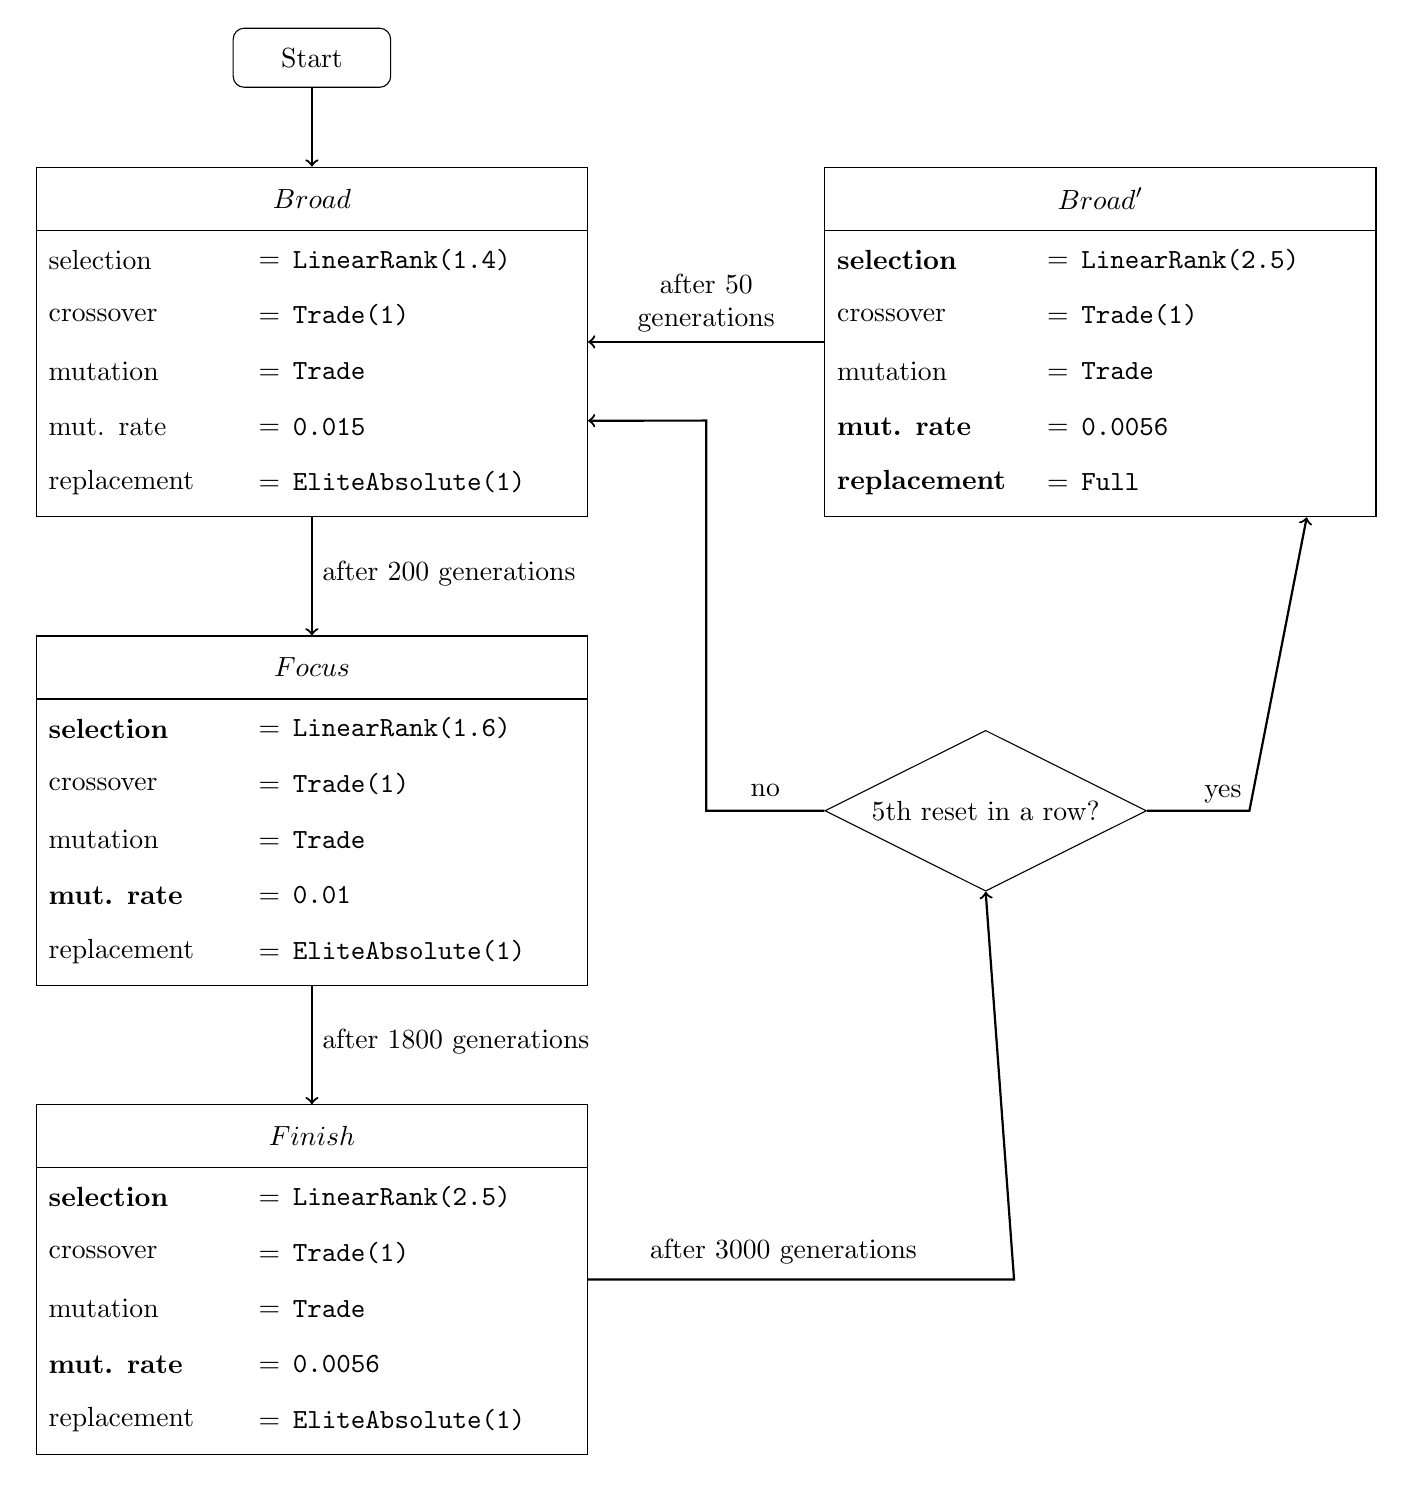
\begin{tikzpicture}
    \tikzstyle{startstop} = [
        rectangle, rounded corners, text centered, draw=black,
        minimum width=2cm, minimum height=0.75cm
    ]

    \tikzstyle{outer} = [
        rectangle, text centered, draw,
        minimum width=7cm, minimum height=4.44cm,
        % inner sep=0pt
    ]
    \tikzstyle{title} = [
        rectangle, text centered, draw,
        minimum width=7cm, minimum height=0.8cm
    ]
    \tikzstyle{param} = [
        rectangle, text centered, %draw,
        align=left,
        minimum width=2.8cm, minimum height=0.7cm,
        text width=2.5cm,
        inner sep=0
    ]
    \tikzstyle{eq} = [
        rectangle, text centered, %draw,
        align=center,
        minimum width=0.3cm, minimum height=0.7cm,
        text width=0.27cm,
        inner sep=0,
        text height=1.4ex
    ]
    \tikzstyle{value} = [
        rectangle, text centered, %draw,
        align=left,
        minimum width=3.8cm, minimum height=0.7cm,
        text width=3.5cm,
        inner sep=0
    ]

    \tikzstyle{decision} = [
        diamond, text centered, draw=black,
        minimum width=3cm, minimum height=1cm, aspect=2
    ]

    %%%%%%%%%%%%%%%%%%%%%%%%%%%%%%%%%%%%%%%%%%%%%%%%%%%%%%%%%%%%%%%%%%%%%%%%%%%%

    \node (start) [startstop] {Start};

    \node (broad_outer) [outer, below=1cm of start] {};
    \node (broad_title) [title, below=0 of broad_outer.north] {$Broad$};

    \matrix
        [column sep=0mm, row sep=0mm] at
        ([yshift=-0.70cm, xshift=-0.11cm]broad_outer.north west)
        [anchor=north west] {
        \node[param] {selection};
            & \node[eq] {$=$};
            & \node[value] {\texttt{LinearRank(1.4)}}; \\

        \node[param] {crossover};
            & \node[eq] {$=$};
            & \node[value] {\texttt{Trade(1)}}; \\

        \node[param] {mutation};
            & \node[eq] {$=$};
            & \node[value] {\texttt{Trade}}; \\

        \node[param] {mut. rate};
            & \node[eq] {$=$};
            & \node[value] {\texttt{0.015}}; \\

        \node[param] {replacement};
            & \node[eq] {$=$};
            & \node[value] {\texttt{EliteAbsolute(1)}};\\
    };

    \node (focus_outer) [outer, below=1.5cm of broad_outer] {};
    \node (focus_title) [title, below=0 of focus_outer.north] {$Focus$};

    \matrix
        [column sep=0mm, row sep=0mm] at
        ([yshift=-0.70cm, xshift=-0.11cm]focus_outer.north west)
        [anchor=north west] {
        \node[param] {\textbf{selection}};
            & \node[eq] {$=$};
            & \node[value] {\texttt{LinearRank(1.6)}}; \\

        \node[param] {crossover};
            & \node[eq] {$=$};
            & \node[value] {\texttt{Trade(1)}}; \\

        \node[param] {mutation};
            & \node[eq] {$=$};
            & \node[value] {\texttt{Trade}}; \\

        \node[param] {\textbf{mut. rate}};
            & \node[eq] {$=$};
            & \node[value] {\texttt{0.01}}; \\

        \node[param] {replacement};
            & \node[eq] {$=$};
            & \node[value] {\texttt{EliteAbsolute(1)}};\\
    };

    \node (finish_outer) [outer, below=1.5cm of focus_outer] {};
    \node (finish_title) [title, below=0 of finish_outer.north] {$Finish$};

    \matrix
        [column sep=0mm, row sep=0mm] at
        ([yshift=-0.70cm, xshift=-0.11cm]finish_outer.north west)
        [anchor=north west] {
        \node[param] {\textbf{selection}};
            & \node[eq] {$=$};
            & \node[value] {\texttt{LinearRank(2.5)}}; \\

        \node[param] {crossover};
            & \node[eq] {$=$};
            & \node[value] {\texttt{Trade(1)}}; \\

        \node[param] {mutation};
            & \node[eq] {$=$};
            & \node[value] {\texttt{Trade}}; \\

        \node[param] {\textbf{mut. rate}};
            & \node[eq] {$=$};
            & \node[value] {\texttt{0.0056}}; \\

        \node[param] {replacement};
            & \node[eq] {$=$};
            & \node[value] {\texttt{EliteAbsolute(1)}}; \\
    };

    \node (broad2_outer) [outer, right=3cm of broad_outer] {};
    \node (broad2_title) [title, below=0 of broad2_outer.north] {$Broad '$};
    \matrix
        [column sep=0mm, row sep=0mm] at
        ([yshift=-0.70cm, xshift=-0.11cm]broad2_outer.north west)
        [anchor=north west] {
        \node[param] {\textbf{selection}};
            & \node[eq] {$=$};
            & \node[value] {\texttt{LinearRank(2.5)}}; \\

        \node[param] {crossover};
            & \node[eq] {$=$};
            & \node[value] {\texttt{Trade(1)}}; \\

        \node[param] {mutation};
            & \node[eq] {$=$};
            & \node[value] {\texttt{Trade}}; \\

        \node[param] {\textbf{mut. rate}};
            & \node[eq] {$=$};
            & \node[value] {\texttt{0.0056}}; \\

        \node[param] {\textbf{replacement}};
            & \node[eq] {$=$};
            & \node[value] {\texttt{Full}}; \\
    };

    \node (branch)
        [decision, right=3cm of focus_outer.east]
        {5th reset in a row?};


    \draw[->, thick]
        (start.south) -- (broad_outer.north);
        % node[midway, right, yshift=0.04cm] {asdf};

    \draw[->, thick]
        (broad_outer.south) -- (focus_outer.north)
        node[midway, right, yshift=0.04cm] {after 200 generations};

    \draw[->, thick]
        (focus_outer.south) -- (finish_outer.north)
        node[midway, right, yshift=0.04cm] {after 1800 generations};

    \draw[->, thick]
        (finish_outer.east)
        -- ++(5.41cm,0)
        -- (branch.south)
        node[midway, above, xshift=-2.75cm, yshift=-2.4cm]
        {after 3000 generations};

    \draw[->, thick]
        (branch.west)
        -- ++(-1.5cm,0)
        -- ++(0,4.955cm)
        -- ([yshift=-1.0cm]broad_outer.east)
        node[midway, above, xshift=1.5cm, yshift=-4.9cm]
        {no};

    \draw[->, thick]
        (branch.east)
        -- ++(1.3cm,0)
        -- ([xshift=2.62cm]broad2_outer.south)
        node[midway, above, xshift=-0.7cm, yshift=-1.9cm]
        {yes};

    \draw[->, thick]
        (broad2_outer.west) -- (broad_outer.east)
        node[midway, above, align=center]
        {after 50\\generations};


\end{tikzpicture}

        \caption{
            \textit{State Machine} self-parameterization method with parameters
            of its direct encoding variant.
        }
        \label{fig:state_machine}
    \end{adjustwidth}
\end{figure}


\subsection{Cosine Mutation Rate}
\label{CosineMutationRate}
The \textit{MutRateCos} dynamic adjusts the mutation rate strictly according to
a cosine waveform. This cyclical behavior allows the mutation rate to oscillate
between higher and lower values, introducing periodic bursts of diversity.
The dynamic is parameterized as follows:
\begin{enumerate}
    \item   \textit{Default mutation rate} ($a$): sets the $y$-axis shift of
            the cosine function, which defines the mutation rate dependent on
            the current generation

    \item   \textit{Amplitude} ($b$): specifies the amplitude of the underlying
            cosine function, effectively determining the maximum deviation the
            mutation rate should undergo compared to the default mutation rate

    \item   \textit{Wavelength} ($c$): defines the wavelength of the underlying
            cosine function in generations

    \item   \textit{Min/max-limit} ($d_{min}, d_{max}$): the last parameter
            allows to restrict the maximum deviation of the mutation rate,
            which is specified by the default mutation rate and the amplitude
            parameters, on either side of the spectrum if desired
\end{enumerate}
These parameters enable fine-tuning of the mutation rate's range and frequency,
ensuring that the dynamic aligns with the algorithm's objectives.
Figure \ref{fig:mut_rate_cos} shows how the parameters affect the mutation
rate over the course of generations.
\begin{figure}[]
    \centering
    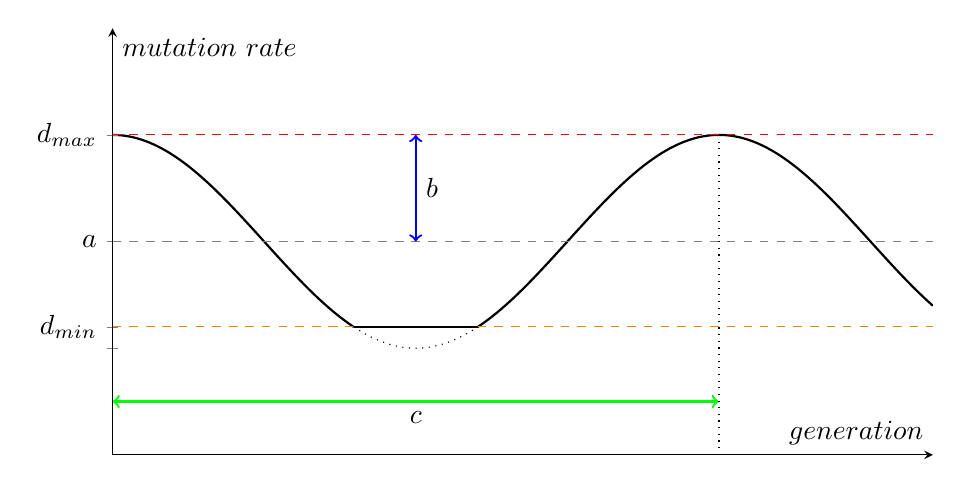
\begin{tikzpicture}
    \begin{axis}[
        axis lines=middle, % Draw axes
        xlabel={$generation$}, % Label x-axis
        ylabel={$mutation$ $rate$}, % Label y-axis
        domain=0:8.5, % Domain for cosine wave (1.5 wavelength)
        xmin=0, xmax=8.5, % Adjust x-axis range
        ymin=0, ymax=4.0, % Adjust y-axis range
        xtick=\empty, % Remove automatic x-ticks
        ytick={1, 1.2, 2, 3}, % Set custom y-ticks
        yticklabels={, $d_{min}$, $a$, $d_{max}$}, % Custom labels for y-ticks
        samples=100, % Number of samples for smooth curve
        width=12cm, % Width of the plot
        height=7cm, % Height of the plot
        axis on top % ensures that the axis are rendered on top
        % smooth, % Smooth curves
    ]

        % Cosine wave with "dent"
        \addplot[black, thick, domain=0:2.49809] {cos(deg(x)) + 2};
        \addplot[black, dotted, domain=2.49809:3.78509] {cos(deg(x)) + 2};
        \addplot[black, thick, domain=3.78509:8.5] {cos(deg(x)) + 2};

        \addplot[black, thick, domain=2.49809:3.78509] {1.2};

        % Draw dashed lines for d_max and d_min
        \addplot[red, dashed] {3};
        \addplot[orange, dashed, domain=0:2.49809] {1.2};
        \addplot[orange, dashed, domain=3.78509:8.5] {1.2};

        % Draw dashed lines for middle
        \addplot[gray, dashed] {2};

        % Mark amplitude
        \draw[<->, blue, thick]
            (axis cs:3.14159,2.0) -- (axis cs:3.14159,3.0)
            node[midway, right, black] {$b$};

        % Mark wavelength
        \draw[<->, green, thick]
            (axis cs:0,0.5) -- (axis cs:6.2832,0.5)
            node[midway, below, black] {$c$};

        \draw[-, dotted]
            (axis cs:6.2832,3.0) -- (axis cs:6.2832,0.0);

        % Add annotations for minima
        % \node[anchor=east] at (axis cs:1.0472, 0) {$d_{min}$};
        % \node[anchor=east] at (axis cs:3.14159, 0) {$d_{min}$};
        % \node[anchor=east] at (axis cs:5.236, 0) {$d_{min}$};
    \end{axis}

\end{tikzpicture}

    \caption{
        Parameters of the \textit{MutRateCos} self-parameterization method.
    }
    \label{fig:mut_rate_cos}
\end{figure}

As this dynamic only modifies the mutation rate, it is compatible with both
direct and indirect encodings and can be applied universally across different
mutation methods.


\subsection{Variable Mutation Rate targeting Mean Cost}
\label{VarMutRateTargetMeanSin}
This dynamic is called \textit{VarMutRateTargetMeanSin} and introduces a more
advanced approach of self-parameterization, which adapts the mutation rate
to reach a target mean objective value of the population. Thereby the target
mean objective value is not constant, but changes dynamically based the mean
objective value of the current generation and a target deviation from that
value given by a sine function.
To achieve the desired mean, this self-parameterization method adjusts the
mutation rate using a PT2 transfer function. The controller continuously
adjusts the mutation rate to steer the population towards the target mean.
To configure these components of this dynamic, it takes the following
parameters:
\begin{enumerate}
    \item   \textit{Average deviation from the current best} ($d$): defines the
            zero-line of the underlying sine wave, which defines the dynamic
            target objective value, relative to the current best objective
            value
    \item   \textit{Gain} ($g$): sets the gain of the PT2 transfer function
    \item   \textit{Amplitude} ($a$): specifies the amplitude of the sine wave,
            which defines the target objective value
    \item   \textit{Wavelength} ($w$): defines the wavelength of the underlying
            sine function in generations
\end{enumerate}

To complement the description provided above, algorithm
\ref{alg:var_mut_rate_target_mean_sin} offers a clearer depiction of the
computational steps involved in the \textit{VarMutRateTargetMeanSin} dynamic.

\begin{algorithm}
    \caption{
        Mutation Rate Adaption targeting dynamic Mean Objective Value
    }
    \label{alg:var_mut_rate_target_mean_sin}

    \begin{algorithmic}
        % Requirements %
        \REQUIRE $d,g,a,w \gets$ parameters (see \ref{VarMutRateTargetMeanSin})
        \REQUIRE $curr_{best}, curr_{mean} \gets$ current best/mean objective
            value
        \REQUIRE $x \gets $ current generation

        % Algorithm %
        \STATE $deviation \gets d + sin_{a,w}(x)$
        \STATE $target \gets curr_{best} \cdot deviation$
        \STATE $diff \gets target - curr_{mean}$

        \STATE $mutationRate \gets mutationRate + PT2_g(diff)$

        \RETURN $mutationRate$

    \end{algorithmic}
\end{algorithm}

Similar to the \textit{Cosine Mutation Rate} (\ref{CosineMutationRate}) dynamic,
this self-parameterization method can also be combined with both the direct
and indirect encoding, as well as used with any mutation method, as it only
modifies the mutation rate, which is always present in a genetic algorithm.


%%%%%%%%%%%%%%%%%%%%%%%%%%%%%%%%%%%%%%%%%%%%%%%%%%%%%%%%%%%%%%%%%%%%%%%%%%%%%%%%
%%% 6. Results                                                               %%%
%%%%%%%%%%%%%%%%%%%%%%%%%%%%%%%%%%%%%%%%%%%%%%%%%%%%%%%%%%%%%%%%%%%%%%%%%%%%%%%%
\chapter{Results}
This chapter presents the results obtained from executing the genetic
algorithms described in this thesis across multiple configurations and on the
two selected problem instances: \textit{hdtt4} and \textit{hdtt5}.
The experiments aimed to evaluate the performance of these algorithms under
various configurations, including the application of the self-parameterization
techniques introduced earlier.

The results are categorized into three primary metrics.
%
The first metric is the \textit{success rate}, which considers whether a given
algorithm configuration could successfully solve the timetabling problem
instance (i.e., achieving a solution with a cost of zero).
%
The second metric examines only the successful runs and evaluates the
\textit{number of generations required} for the algorithm to find a valid
solution.
%
Finally, the third metric focuses on the \textit{performance}, measuring the
computational efficiency of the algorithms in terms of the number of
generations processed per second.

For performing consecutive runs without the need for manual intervention, an
auxiliary application called the \textit{auto runner} was implemented, which
loops through a given set of algorithm configurations, executing them
automatically one after the other.
With this application the algorithm executions could be tested for multiple
days without supervision.
The captured data of all algorithm executions, including success rates, runtime
metrics, and configurations, is openly available in the \textit{GAX-Plots}
repository on GitHub \cite{code-gax-plots}. This repository also contains the
R scripts used to generate the visualizations included in this chapter,
supporting transparency and reproducibility in this research.
These diagrams include abbreviations for the algorithms,
their configurations, and the self-parameterization techniques applied
(if any):

The two genetic algorithms analyzed in this study are referred to as
\texttt{alg\_11} and \texttt{alg\_12}. During the exploration phase of this
research, various algorithms were developed iteratively. The final two
approaches capable of solving timetabling problem instances from the XHSTT
archives were designated as \texttt{alg\_11} and \texttt{alg\_12}.
The former employs the direct encoding scheme, while the latter is based on the
indirect encoding scheme.

The configurations and optional self-parameterization techniques for each
algorithm are shown in abbreviated form in the result plots, because using the
full name of every single algorithm parameter would be too long for displaying
the results in diagrams. All abbreviations used for static algorithm
configurations are shown in table \ref{tab:ga-cfg-abbr}. Similarly, table
\ref{tab:ga-dynamic-abbr} lists the abbreviations of dynamics.

\begin{table}[h!]
    % This table was created with https://www.tablesgenerator.com/latex_tables#
% To edit the table visit the website and import the `.tgn` file from this
% directory.

\begin{adjustwidth}{-3cm}{-3cm}

    \centering
    \begin{tabular}{|l|l|lll|}
    \hline
    \rowcolor[HTML]{DCDCDC} 
    \textbf{Abbr.}                   & \textbf{Description}                                & \multicolumn{3}{l|}{\cellcolor[HTML]{DCDCDC}\textbf{Values}}                                                                                                                                                         \\ \hline
    \texttt{P:}$n$                   & Population Size                                     & \multicolumn{3}{l|}{$n \in \mathbb{N}^+$ (e.g. $n = 1000$)}                                                                                                                                                           \\ \hline
    \texttt{MR:}$x$                  & Mutation Rate                                       & \multicolumn{3}{l|}{$x \in \mathbb{R}^+$ (e.g. $n = 0.01 \hateq 1\%$)}                                                                                                                                                \\ \hline
                                     &                                                     & \multicolumn{1}{l|}{\cellcolor[HTML]{EFEFEF}\textbf{Abbr.}} & \multicolumn{1}{l|}{\cellcolor[HTML]{EFEFEF}\textbf{Description}}                      & \cellcolor[HTML]{EFEFEF}\textbf{Parameters}                   \\ \cline{3-5} 
                                     &                                                     & \multicolumn{1}{l|}{\texttt{rltt-}$x$}                      & \multicolumn{1}{l|}{Roulette Wheel}                                                    &                                                               \\ \cline{3-5} 
                                     &                                                     & \multicolumn{1}{l|}{\texttt{trn-}$n$}                       & \multicolumn{1}{l|}{$n$-Tournament}                                                    & $n$: Tournament Size                                          \\ \cline{3-5} 
    \multirow{-4}{*}{\texttt{SE:\_}} & \multirow{-4}{*}{\makecell[l]{Selection\\Method}}   & \multicolumn{1}{l|}{\texttt{lnrnk-}$x$}                     & \multicolumn{1}{l|}{Linear  Rank}                                                      & $x$: Selection Pressure                                       \\ \hline
                                     &                                                     & \multicolumn{1}{l|}{\cellcolor[HTML]{EFEFEF}\textbf{Abbr.}} & \multicolumn{1}{l|}{\cellcolor[HTML]{EFEFEF}\textbf{Description}}                      & \cellcolor[HTML]{EFEFEF}\textbf{Parameters}                   \\ \cline{3-5} 
                                     &                                                     & \multicolumn{1}{l|}{\texttt{uni}}                           & \multicolumn{1}{l|}{Uniform}                                                           &                                                               \\ \cline{3-5} 
                                     &                                                     & \multicolumn{1}{l|}{\texttt{trd}$n$}                        & \multicolumn{1}{l|}{$n$-Trade}                                                         & \makecell[l]{$n$: Number of Trades}                           \\ \cline{3-5} 
                                     &                                                     & \multicolumn{1}{l|}{\texttt{vspt}}                          & \multicolumn{1}{l|}{Variable Single Point}                                             &                                                               \\ \cline{3-5} 
                                     &                                                     & \multicolumn{1}{l|}{\texttt{v}$n$\texttt{pt}}               & \multicolumn{1}{l|}{Variable $n$-Point}                                                & \makecell[l]{$n$: Number of\\Crossover Points}                \\ \cline{3-5} 
                                     &                                                     & \multicolumn{1}{l|}{\texttt{pmx}}                           & \multicolumn{1}{l|}{PMX}                                                               &                                                               \\ \cline{3-5} 
    \multirow{-7}{*}{\texttt{CX:\_}} & \multirow{-7}{*}{\makecell[l]{Crossover\\Method}}   & \multicolumn{1}{l|}{\texttt{ord}}                           & \multicolumn{1}{l|}{Ordered}                                                           &                                                               \\ \hline
                                     &                                                     & \multicolumn{1}{l|}{\cellcolor[HTML]{EFEFEF}\textbf{Abbr.}} & \multicolumn{1}{l|}{\cellcolor[HTML]{EFEFEF}\textbf{Description}}                      & \cellcolor[HTML]{EFEFEF}\textbf{Parameters}                   \\ \cline{3-5} 
                                     &                                                     & \multicolumn{1}{l|}{\texttt{mvsub}}                         & \multicolumn{1}{l|}{MoveSubEvent}                                                      &                                                               \\ \cline{3-5} 
                                     &                                                     & \multicolumn{1}{l|}{\texttt{mvtime}}                        & \multicolumn{1}{l|}{MoveSingleTimeAlloc}                                               &                                                               \\ \cline{3-5} 
                                     &                                                     & \multicolumn{1}{l|}{\texttt{gauss-mvtime}}                  & \multicolumn{1}{l|}{\makecell[l]{MoveSingleTimeAlloc\\(Gaussian Variant)}}             &                                                               \\ \cline{3-5} 
                                     &                                                     & \multicolumn{1}{l|}{\texttt{trd}}                           & \multicolumn{1}{l|}{Trade}                                                             &                                                               \\ \cline{3-5} 
    \multirow{-6}{*}{\texttt{MU:\_}} & \multirow{-6}{*}{\makecell[l]{Mutation\\Method}}    & \multicolumn{1}{l|}{\texttt{gauss-trd}}                     & \multicolumn{1}{l|}{Trade (Gaussian Variant)}                                          &                                                               \\ \hline
                                     &                                                     & \multicolumn{1}{l|}{\cellcolor[HTML]{EFEFEF}\textbf{Abbr.}} & \multicolumn{1}{l|}{\cellcolor[HTML]{EFEFEF}\textbf{Description}}                      & \cellcolor[HTML]{EFEFEF}\textbf{Parameters}                   \\ \cline{3-5} 
                                     &                                                     & \multicolumn{1}{l|}{\texttt{full}}                          & \multicolumn{1}{l|}{Full Replacement}                                                  &                                                               \\ \cline{3-5} 
                                     &                                                     & \multicolumn{1}{l|}{\texttt{eli-abs-}$n$}                   & \multicolumn{1}{l|}{Absolute Elite}                                                    & $n \in \mathbb{N}$: Elite Size                                \\ \cline{3-5} 
    \multirow{-4}{*}{\texttt{RE:\_}} & \multirow{-4}{*}{\makecell[l]{Replacement\\Method}} & \multicolumn{1}{l|}{\texttt{eli-rel-}$x$}                   & \multicolumn{1}{l|}{\makecell[l]{Elite relative to\\population size}}                  & \makecell[l]{$x \in \mathbb{R}$: Elite Size\\(e.g. $x=1.01$)} \\ \hline
                                     &                                                     & \multicolumn{1}{l|}{\cellcolor[HTML]{EFEFEF}\textbf{Abbr.}} & \multicolumn{1}{l|}{\cellcolor[HTML]{EFEFEF}\textbf{Description}}                      & \cellcolor[HTML]{EFEFEF}\textbf{Parameters}                   \\ \cline{3-5} 
                                     &                                                     & \multicolumn{1}{l|}{\texttt{g-}$n$}                         & \multicolumn{1}{l|}{Stop after $n$-th generation}                                      & $n$: Generation                                               \\ \cline{3-5} 
                                     &                                                     & \multicolumn{1}{l|}{\texttt{ov-}$x$}                        & \multicolumn{1}{l|}{\makecell[l]{Stop if best individual\\has target objective value}} & $x$: Objective Value                                          \\ \cline{3-5} 
    \multirow{-4}{*}{\texttt{TE:\_}} & \multirow{-4}{*}{\makecell[l]{Termination\\Method}} & \multicolumn{1}{l|}{\texttt{g-}$n$\texttt{-ov-}$x$}         & \multicolumn{1}{l|}{Combination of the above}                                          & see above                                                     \\ \hline
    \end{tabular}
    \caption{Abbreviations of genetic algorithm \textit{configurations}.}
    \label{tab:ga-cfg-abbr}

\end{adjustwidth}

\end{table}

\begin{table}[h!]
    % This table was created with https://www.tablesgenerator.com/latex_tables#
% To edit the table visit the website and import the `.tgn` file from this
% directory.
\begin{adjustwidth}{-3cm}{-3cm}
    \centering
    \begin{tabular}{|l|l|l|}
    \hline
    \rowcolor[HTML]{DCDCDC} 
    \textbf{Abbreviation}                                                            & \textbf{Description}                                         & \textbf{Parameters}                             \\ \hline
    \texttt{mut-rate-cos-}$a$\texttt{-}$b$\texttt{-}$c$\texttt{-}$d$                 & Cosine Mutation Rate                                         & see \ref{CosineMutationRate}                    \\ \hline
    \texttt{gauss-rnd-time-}$x$                                                      & Gaussian Random Time                                         & see \ref{GaussianRandomTime}                    \\ \hline
    \texttt{gauss-rnd-evnt-}$x$                                                      & Gaussian Random Event                                        & see \ref{GaussianRandomEvent}                   \\ \hline
    \texttt{var-mut-rate-target-mean-sin-}$a$\texttt{-}$b$\texttt{-}$c$\texttt{-}$d$ & \makecell[l]{Variable Mutation Rate\\targeting a mean value} & see \ref{VarMutRateTargetMeanSin}               \\ \hline
    \texttt{inc-lin-rnk-sel-pressure-}$a$\texttt{-}$b$\texttt{-}$c$\texttt{-}$d$     & \makecell[l]{Increasing Linear Rank\\Selection Pressure}     & see \ref{IncreasingLinearRankSelectionPressure} \\ \hline
    \texttt{state-machine}                                                           & State Machine (\ref{StateMachine})                           &                                                 \\ \hline
    \end{tabular}
    \caption{Abbreviations of genetic algorithm \textit{dynamics}.}
    \label{tab:ga-dynamic-abbr}
\end{adjustwidth}


\end{table}

Using these abbreviations, in combination with a consistent naming scheme,
makes each algorithm configuration identifiable by its unique abbreviated
configuration name, which is crucial for collecting data of multiple
algorithm executions in a structured way, as well as processing this data.

The naming scheme of algorithm configurations and dynamics adheres to the
following scheme:
\begin{itemize}
    \item   \texttt{cfg\_[c]}, if no dynamics are used, where
            \enquote{\texttt{[c]}} is replaced by a list of \enquote{\_}
            delimited configuration abbreviations

    \item   \texttt{cfg\_[c]\_\_\_dyn\_[d]}, if dynamics are used, where
            \enquote{\texttt{[c]}} again stands for a list of configurations,
            and \enquote{\texttt{[d]}} is a placeholder for a \enquote{\_}
            delimited list of used dynamics
\end{itemize}


% Success Rates %%%%%%%%%%%%%%%%%%%%%%%%%%%%%%%%%%%%%%%%%%%%%%%%%%%%%%%%%%%%%%%%
\section{Success Rates}
The success rates of the genetic algorithms developed in this study were
evaluated on both the \textit{hdtt4} and \textit{hdtt5} problem instances.
Each algorithm was executed multiple times with different configurations,
and the success rate of every algorithm configuration was calculated as the
proportion of successful runs, meaning the algorithm found a zero cost solution.

For the \textit{hdtt4} problem instance, the results for the two algorithms
differ notably. With the direct encoding scheme, which is employed by
\texttt{alg\_11}, none of the tested \textit{static} configurations were
always successful (see figure \ref{fig:alg_11_static_hdtt4_success_rates}).
%
\begin{figure}[hb!]
    \begin{adjustwidth}{-3cm}{-3cm}
        \centering
        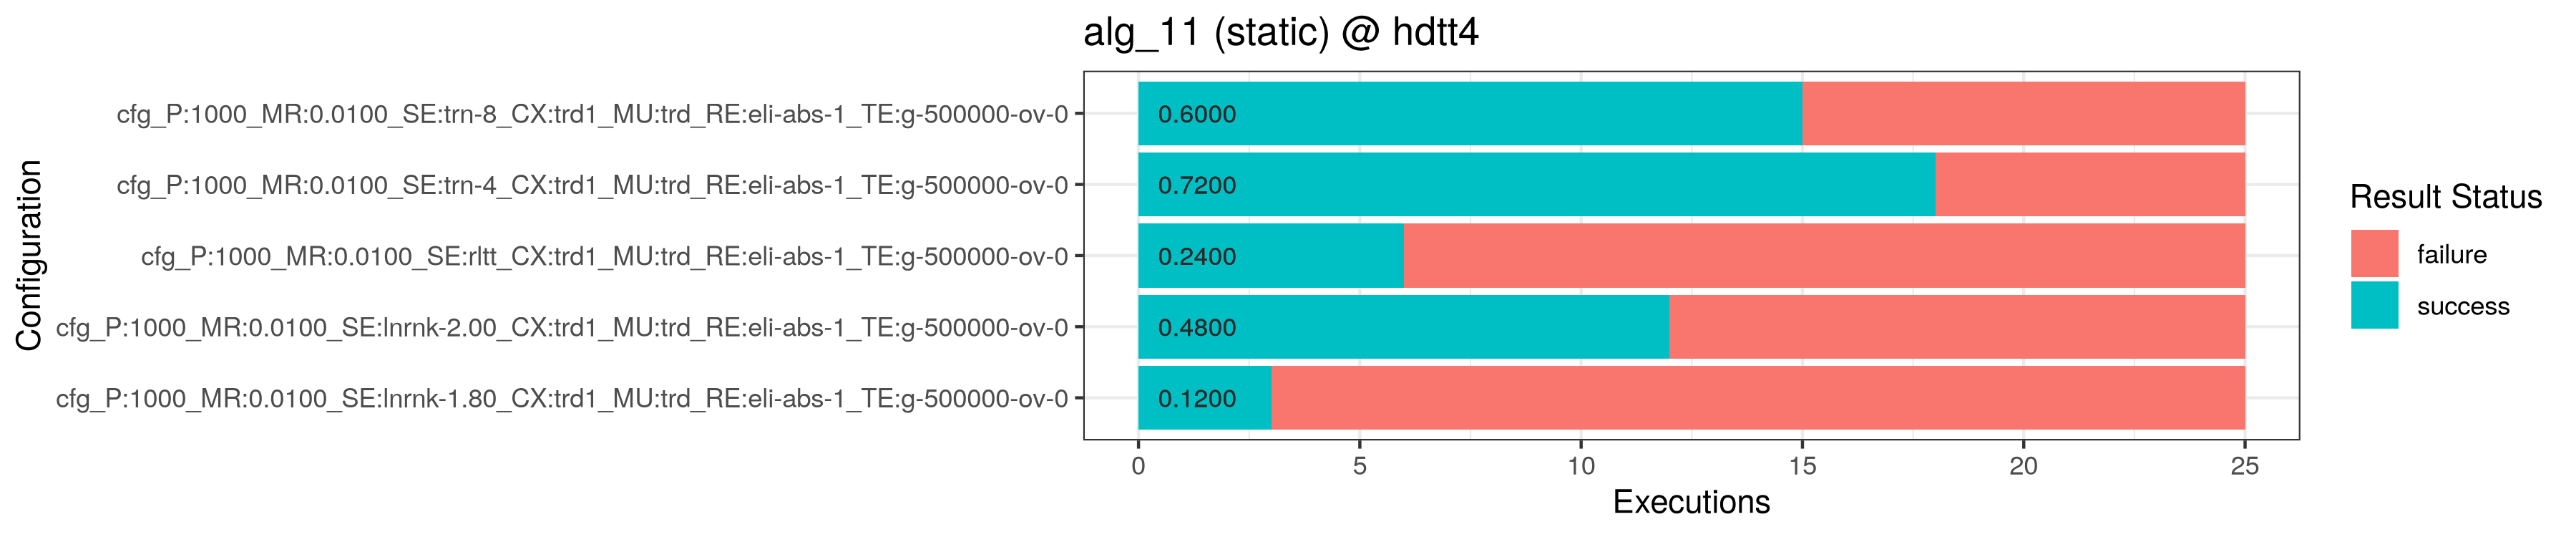
\includegraphics[width=1.28\textwidth]{assets/chap-6/success-rates/hdtt4/alg_11/static_success_rate.png}
        \caption{
            Success Rates of \texttt{alg\_11} without dynamics on \textit{hdtt4}
            instances.
        }
        \label{fig:alg_11_static_hdtt4_success_rates}
    \end{adjustwidth}
\end{figure}

By incorporating the \textit{State Machine} (see \ref{StateMachine})
self-parameterization method, the algorithm using the direct encoding was
consistently able to find valid timetables
(see figure \ref{fig:alg_11_dynamic_hdtt4_success_rates}).
%
\begin{figure}[hb!]
    \begin{adjustwidth}{-3cm}{-3cm}
        \centering
        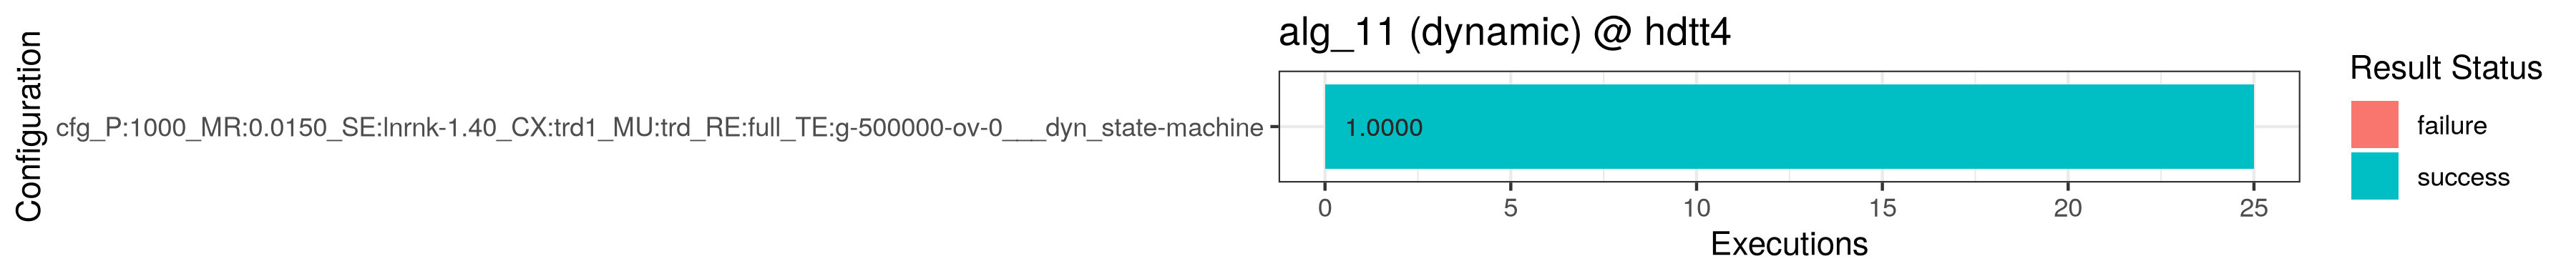
\includegraphics[width=1.28\textwidth]{assets/chap-6/success-rates/hdtt4/alg_11/dynamic_success_rate.png}
        \caption{
            Success rates of \texttt{alg\_11} with dynamics on \textit{hdtt4}
            instances.
        }
        \label{fig:alg_11_dynamic_hdtt4_success_rates}
    \end{adjustwidth}
\end{figure}

The reason for only including one single configuration utilizing
self-parameterization is, that during development of the dynamics for the
direct encoding, none of the other self-parameterization methods showed
significant improvements compared to statically configured algorithms.
As the repetitive execution of configurations which are likely to fail
is very time-consuming, because these runs are terminated by a generation limit,
the tests for self-parameterized algorithms with direct encoding were
only executed for the state machine dynamic.

In contrast, \texttt{alg\_12}, which uses the indirect encoding scheme,
demonstrated strong performance with both static and dynamic configurations,
achieving a 100\% success rate with multiple setups
(see figure \ref{fig:alg_12_static_hdtt4_success_rates} and
\ref{fig:alg_12_dynamic_hdtt4_success_rates}).
%
\begin{figure}[h!]
    \begin{adjustwidth}{-3cm}{-3cm}
        \centering
        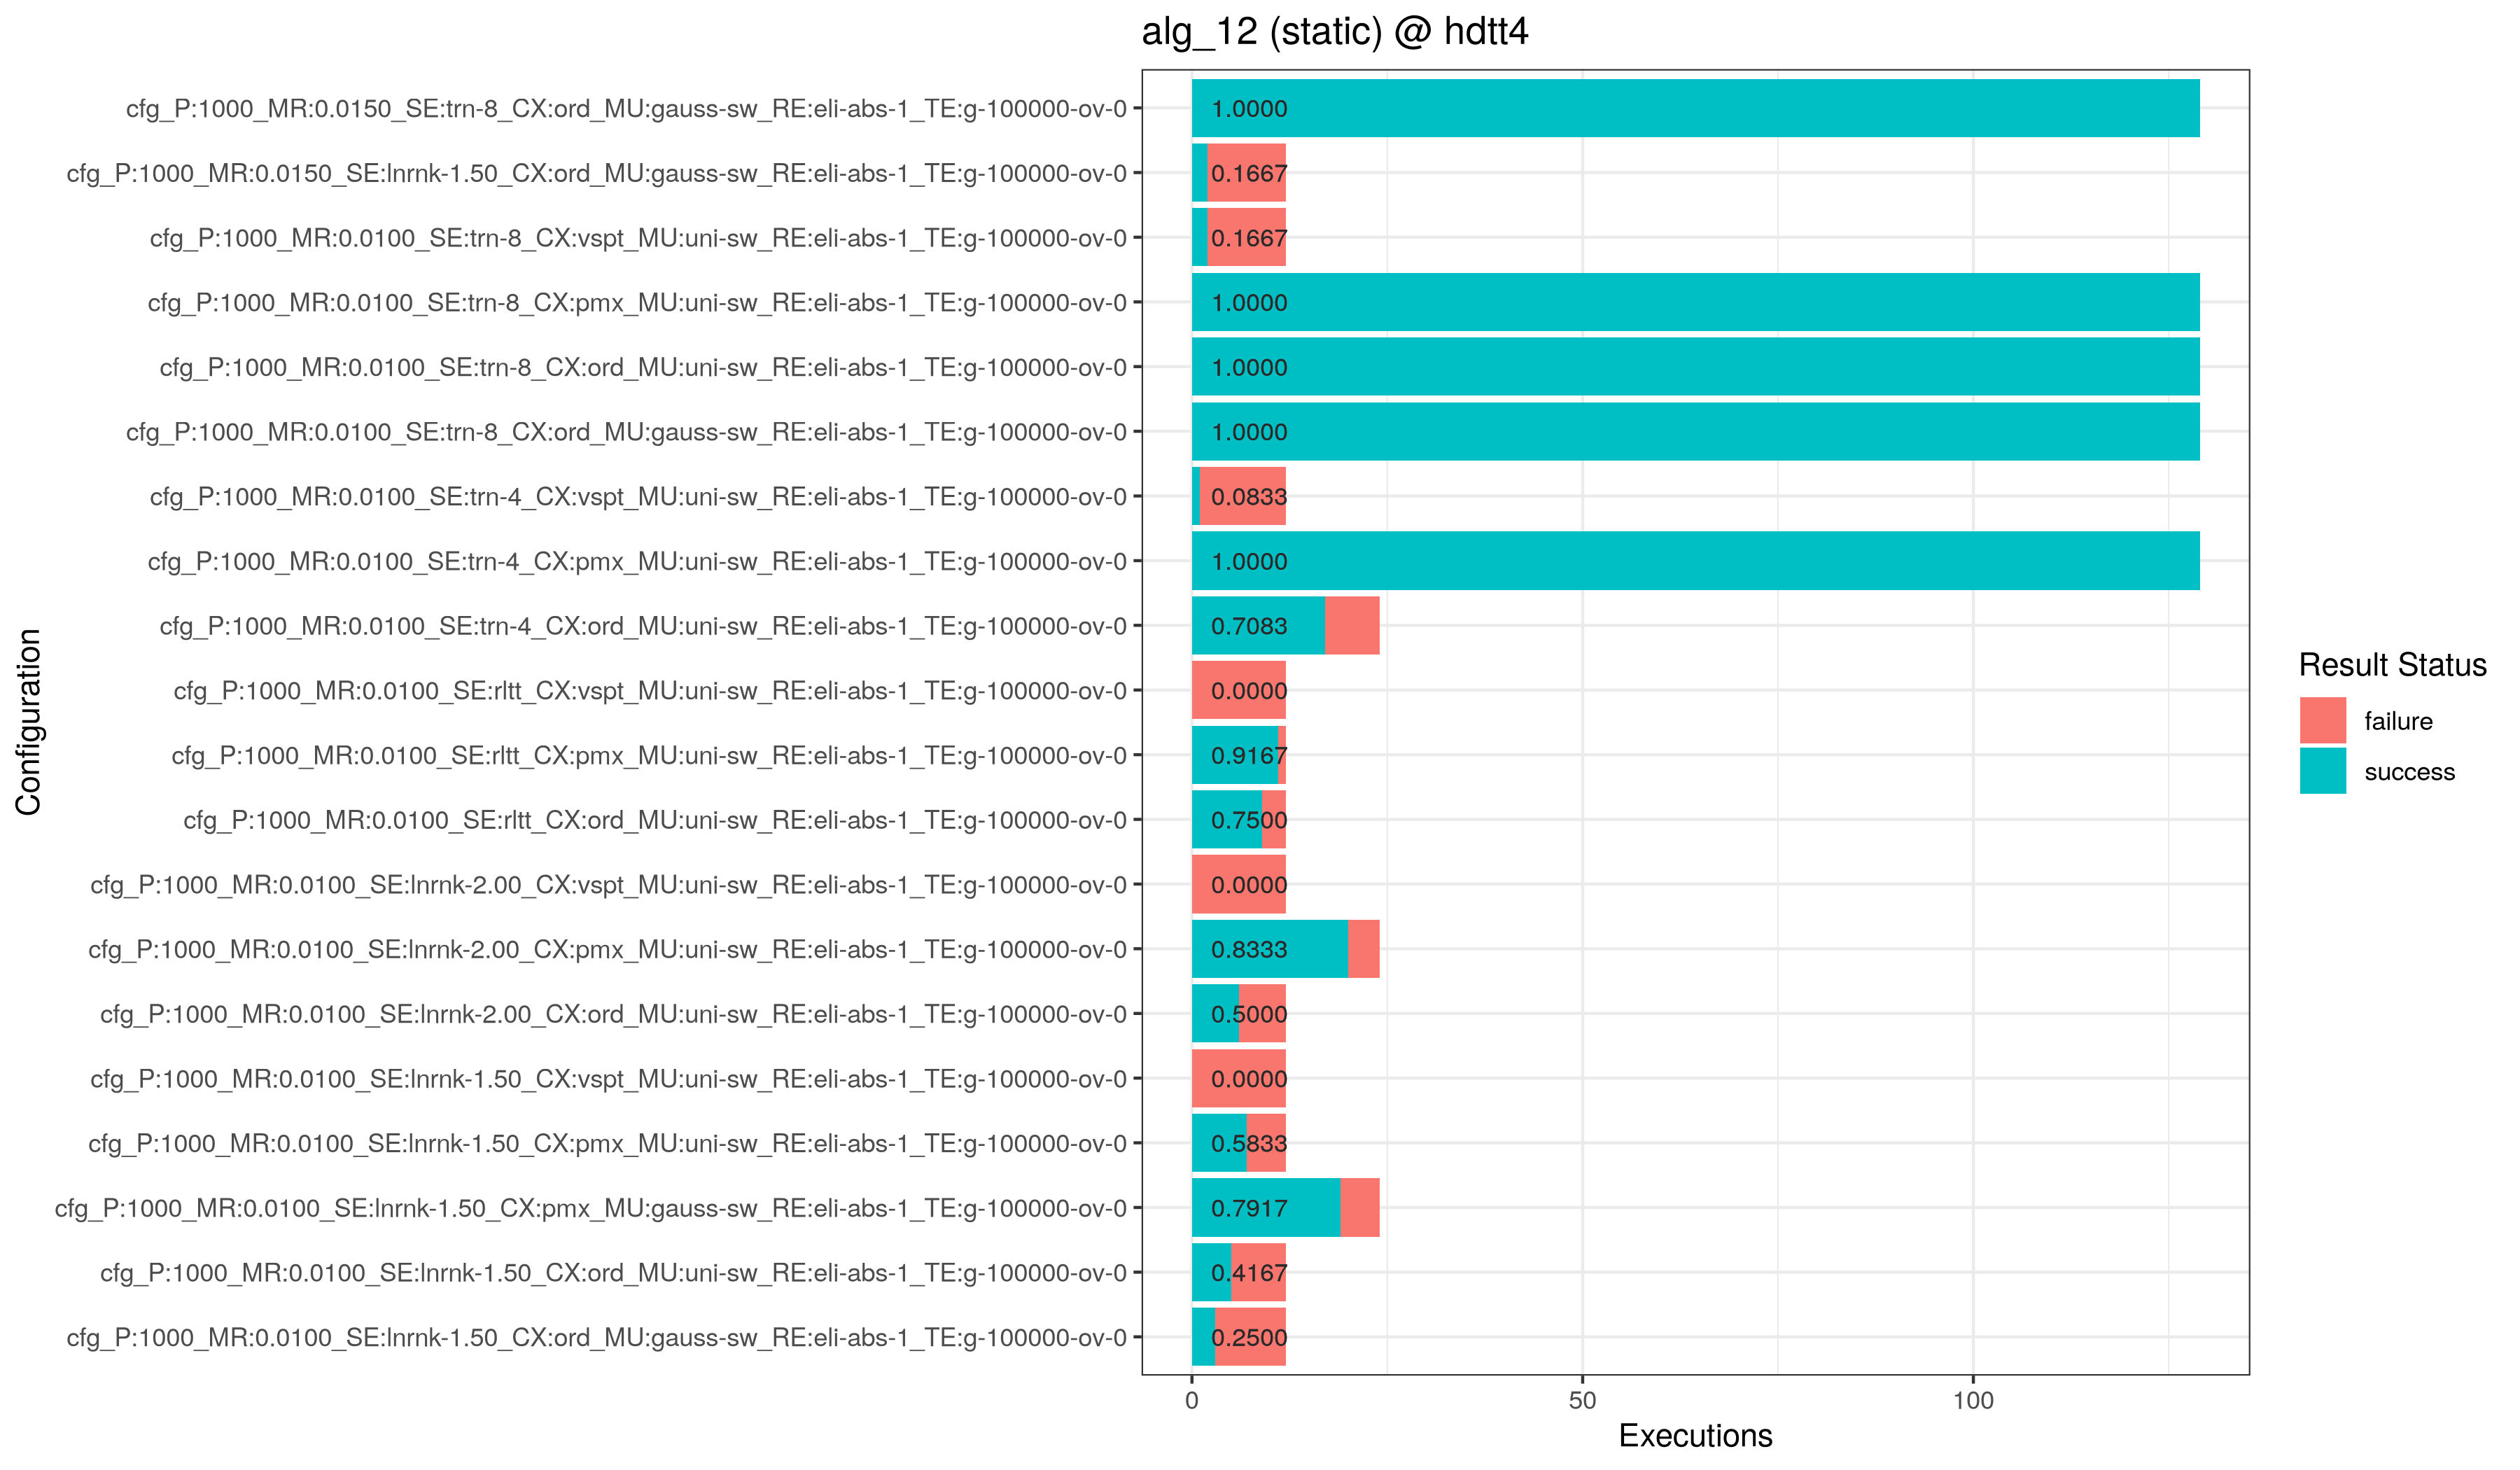
\includegraphics[width=1.28\textwidth]{
            assets/chap-6/success-rates/hdtt4/alg_12/static_success_rate.png
        }
        \caption{
            Success rates of \texttt{alg\_12} without dynamics on \textit{hdtt4}
            instances.
        }
        \label{fig:alg_12_static_hdtt4_success_rates}
    \end{adjustwidth}
\end{figure}
%
\begin{figure}[h!]
    \begin{adjustwidth}{-3cm}{-3cm}
        \centering
        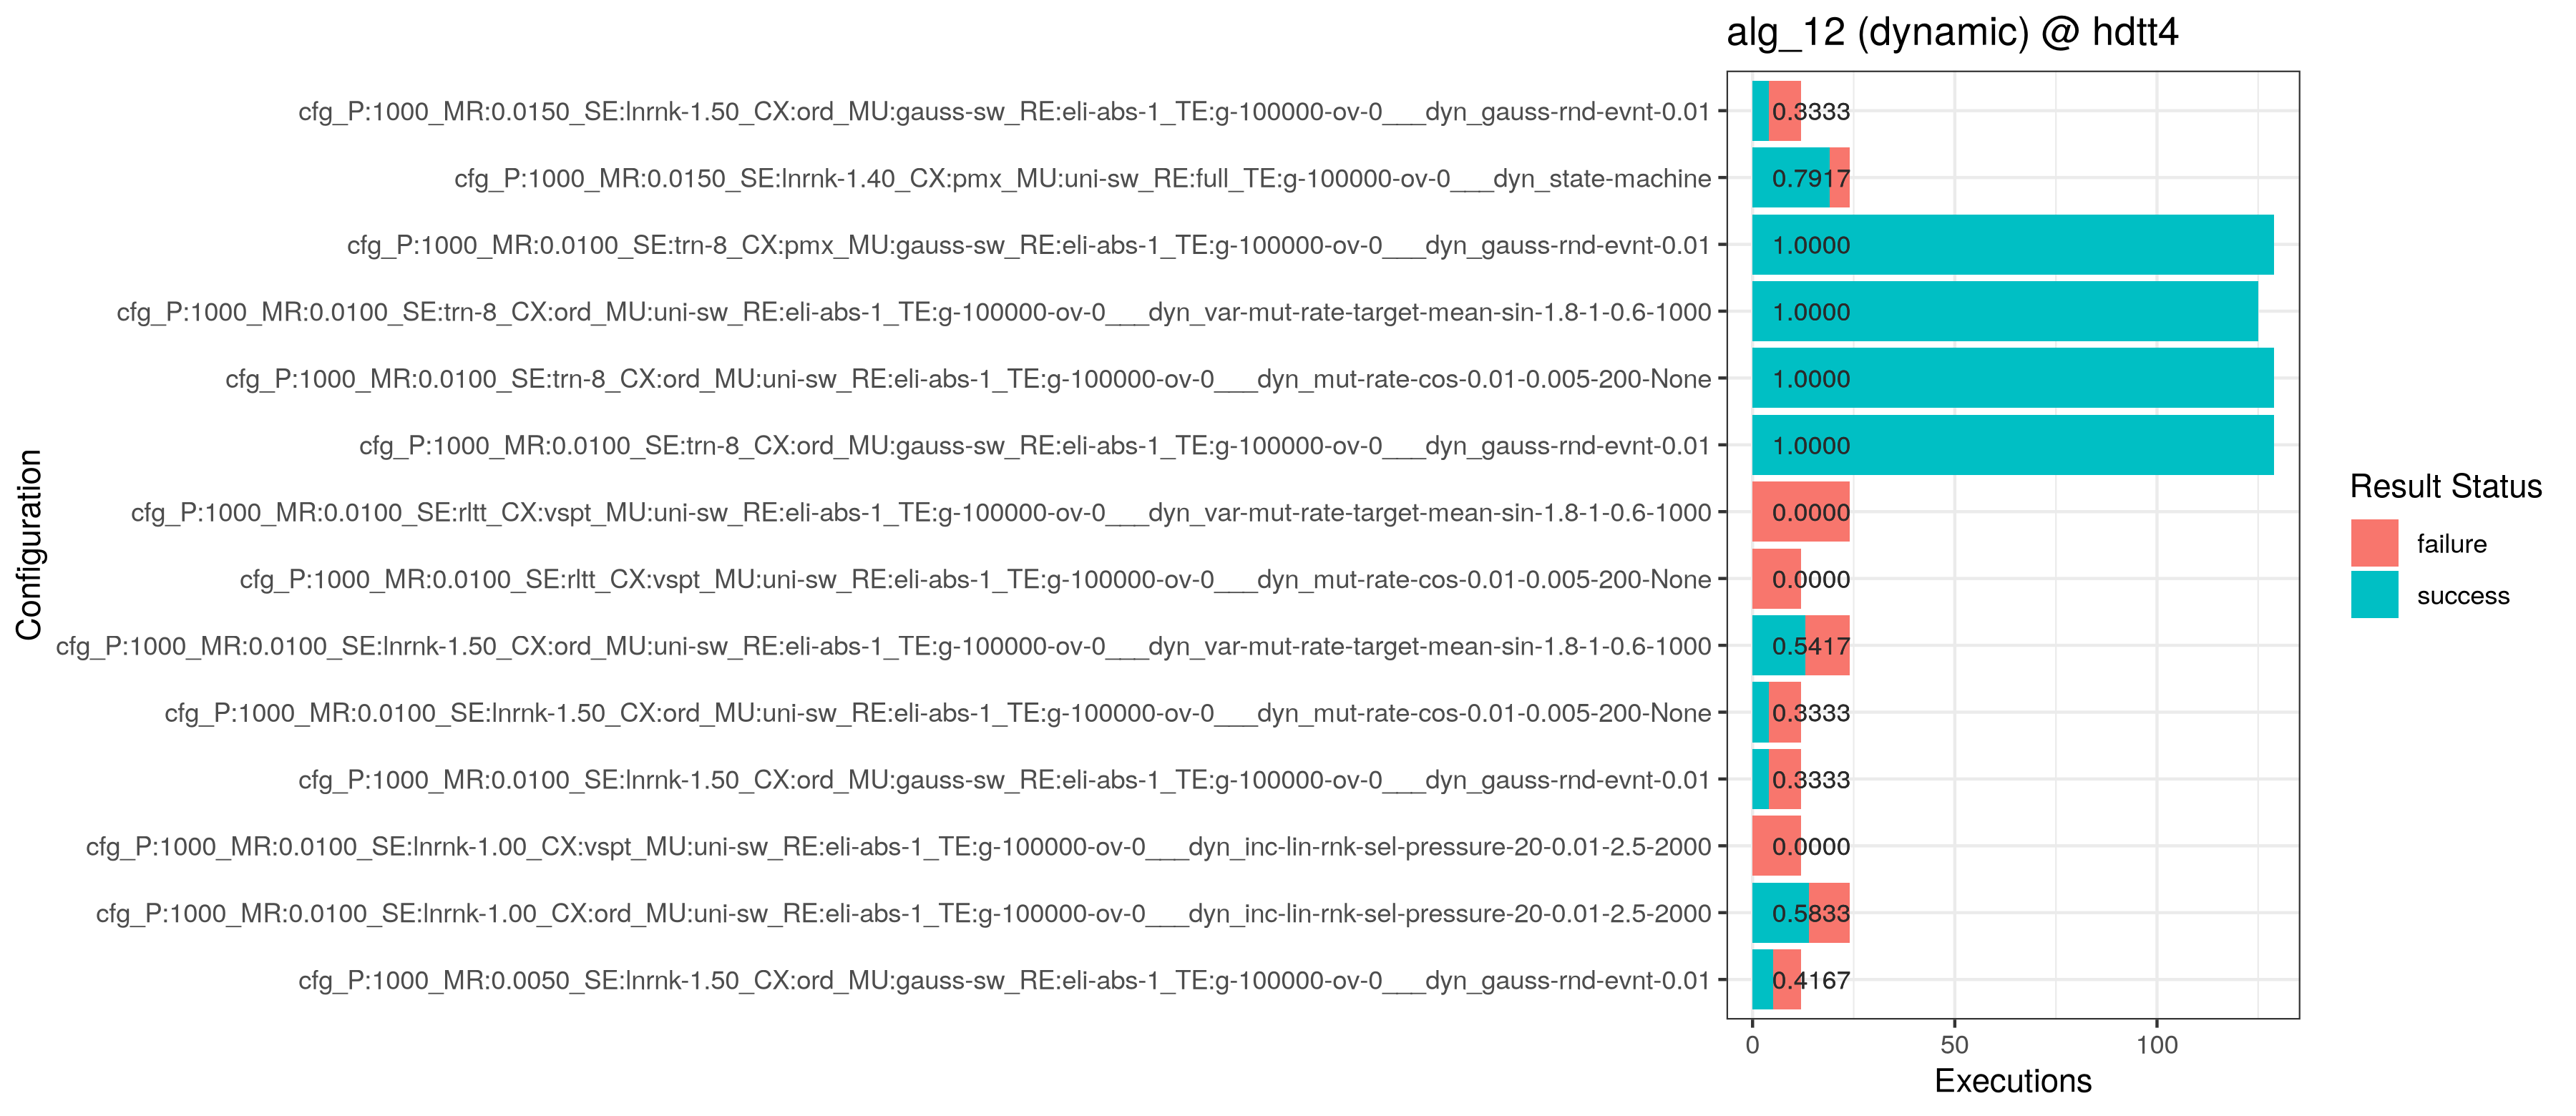
\includegraphics[width=1.28\textwidth]{
            assets/chap-6/success-rates/hdtt4/alg_12/dynamic_success_rate.png
        }
        \caption{
            Success rates of \texttt{alg\_12} with dynamics on \textit{hdtt4}
            instances.
        }
        \label{fig:alg_12_dynamic_hdtt4_success_rates}
    \end{adjustwidth}
\end{figure}

For solving the \textit{hdtt5} problem instance, only \texttt{alg\_12} was
executed because none of the tested configurations of the \texttt{alg\_11}
algorithm were able to solve this problem instance.
Among the static configurations, only one managed to achieve a 100\% success
rate.
Interestingly, none of the dynamic configurations reached this level of success
for \textit{hdtt5}.
Figures \ref{fig:alg_12_static_hdtt5_success_rates} and
\ref{fig:alg_12_dynamic_hdtt5_success_rates} present the success rates for the
hdtt5 problem instances, offering a comparative visualization of static and
dynamic configurations.
%
\begin{figure}[h!]
    \begin{adjustwidth}{-3cm}{-3cm}
        \centering
        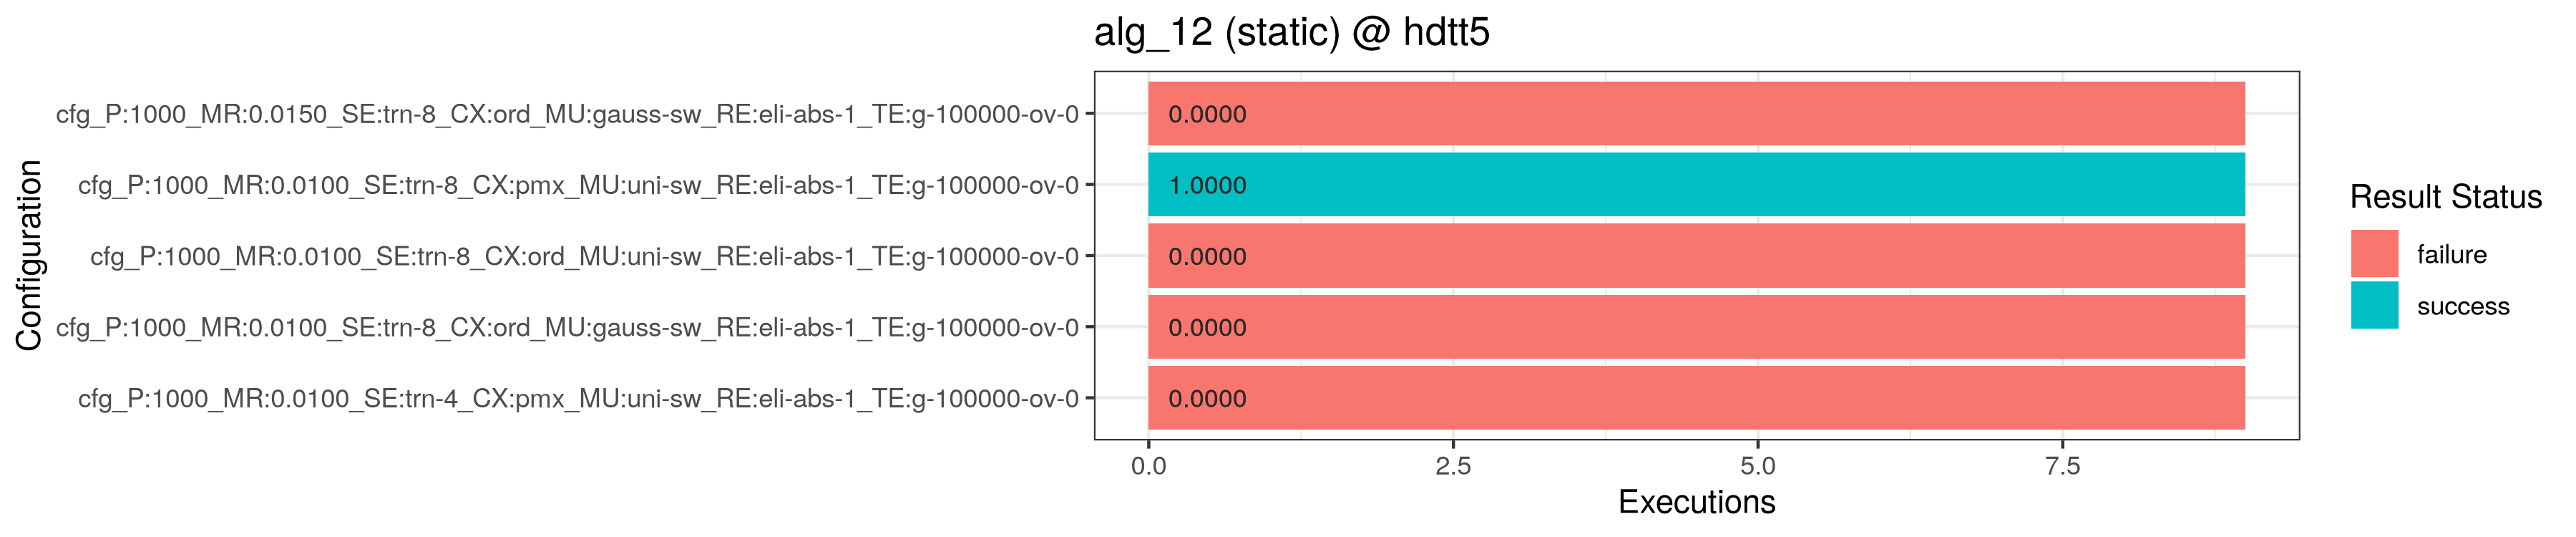
\includegraphics[width=1.28\textwidth]{
            assets/chap-6/success-rates/hdtt5/alg_12/static_success_rate.png
        }
        \caption{
            Success rates of \texttt{alg\_12} without dynamics on \textit{hdtt5}
            instances.
        }
        \label{fig:alg_12_static_hdtt5_success_rates}
    \end{adjustwidth}
\end{figure}
%
\begin{figure}[h!]
    \begin{adjustwidth}{-3cm}{-3cm}
        \centering
        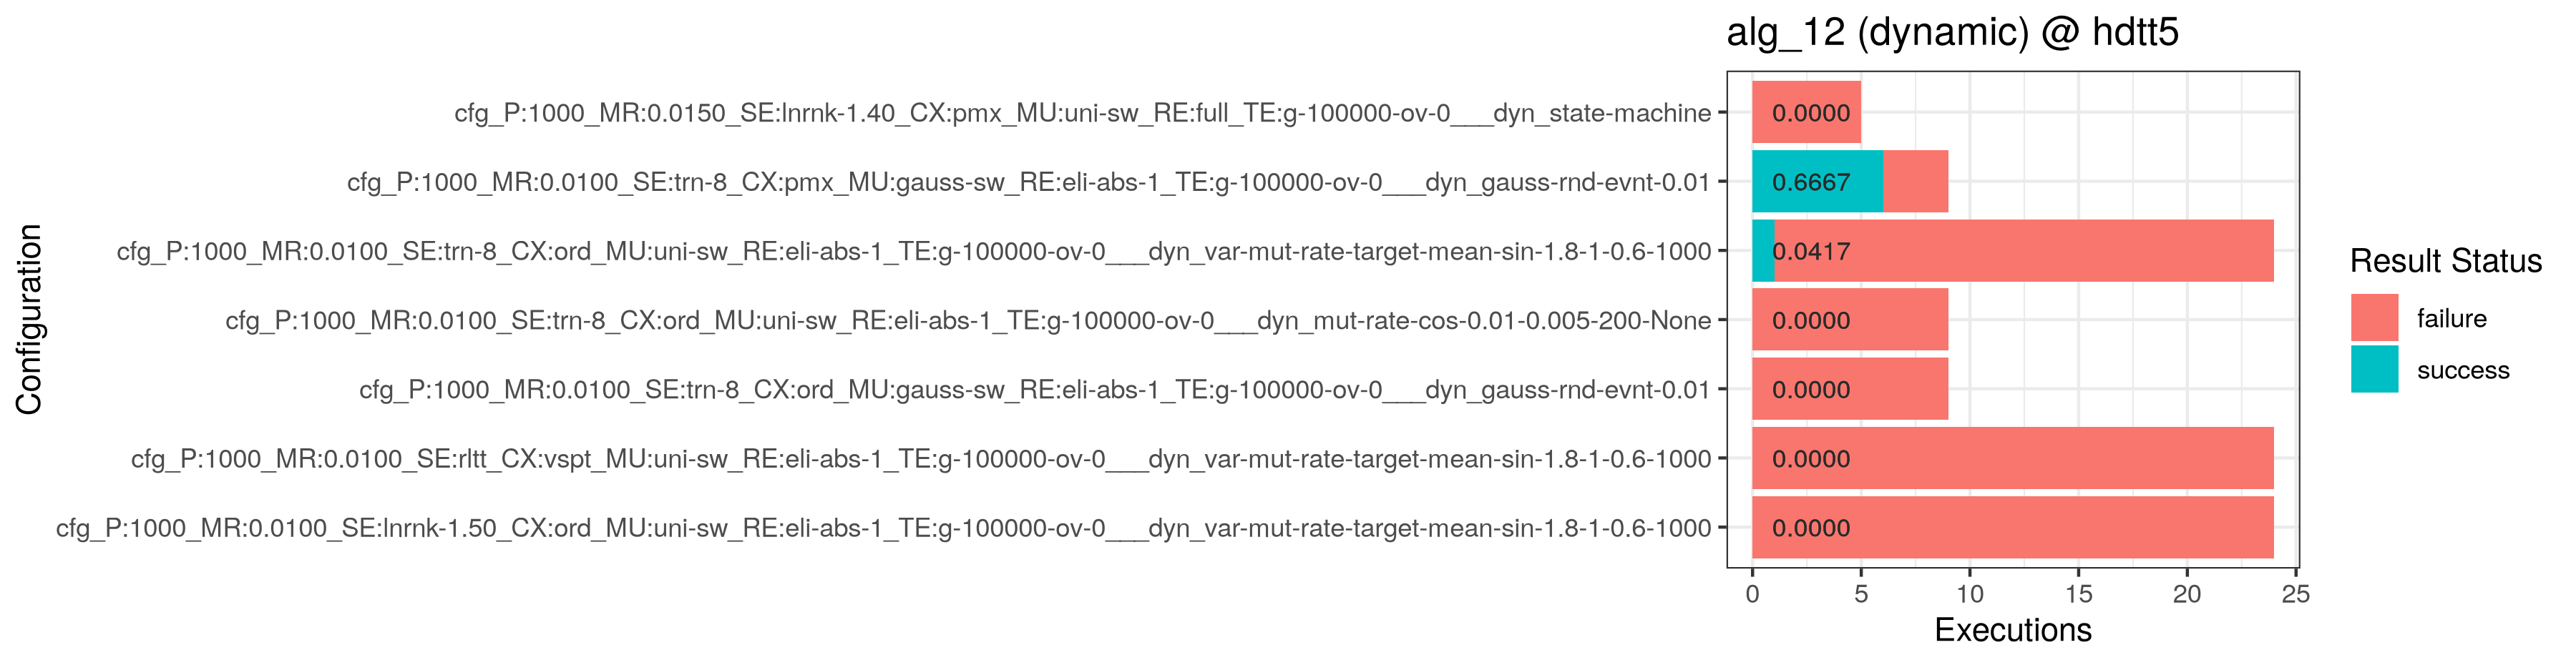
\includegraphics[width=1.28\textwidth]{
            assets/chap-6/success-rates/hdtt5/alg_12/dynamic_success_rate.png
        }
        \caption{
            Success rates of \texttt{alg\_12} with dynamics on \textit{hdtt5}
            instances.
        }
        \label{fig:alg_12_dynamic_hdtt5_success_rates}
    \end{adjustwidth}
\end{figure}
\newpage

% Number of Generations until Success %%%%%%%%%%%%%%%%%%%%%%%%%%%%%%%%%%%%%%%%%%
\section{Number of Generations taken on Success}
The number of generations required to find a valid solution was another
critical metric analyzed in this study. These results, which only consider
successful runs, provide insights into the computational effort needed to solve
the problem instances. Restricting the scope of this metric to only include
algorithm executions which found valid timetables prevents the resulting
data from being distorted towards the maximum number of generations allowed
for each execution. Additionally, algorithm configurations with a success rate
of 100\% are highlighted by distinct coloring.


Algorithm \texttt{alg\_11} executed on the \textit{hdtt4} instance, yields
results which show a correlation of a configuration's success rate and the
number of generations it takes on successful runs.
One of the static configurations stands out by taking fewer generations
to find a valid timetable than all the other configurations, despite having the
lowest success rate among the others (figure
\ref{fig:alg_11_static_hdtt4_generations_taken}).
For the other static configurations having better success rates correlates
with also on average taking more generations to succeed.
In comparison, the corresponding dynamic configuration is comparable
to its static counterparts regarding the generations taken, but simultaneously
provides perfect reliability (figure
\ref{fig:alg_11_dynamic_hdtt4_generations_taken}).
%
% In conclusion the amount of generations taken presented by the dynamic
% configuration is on par with the static configurations in this regard,
% especially when taking these configurations' success rates into consideration.
%
\begin{figure}[h]
    \begin{adjustwidth}{-3cm}{-3cm}
        \centering
        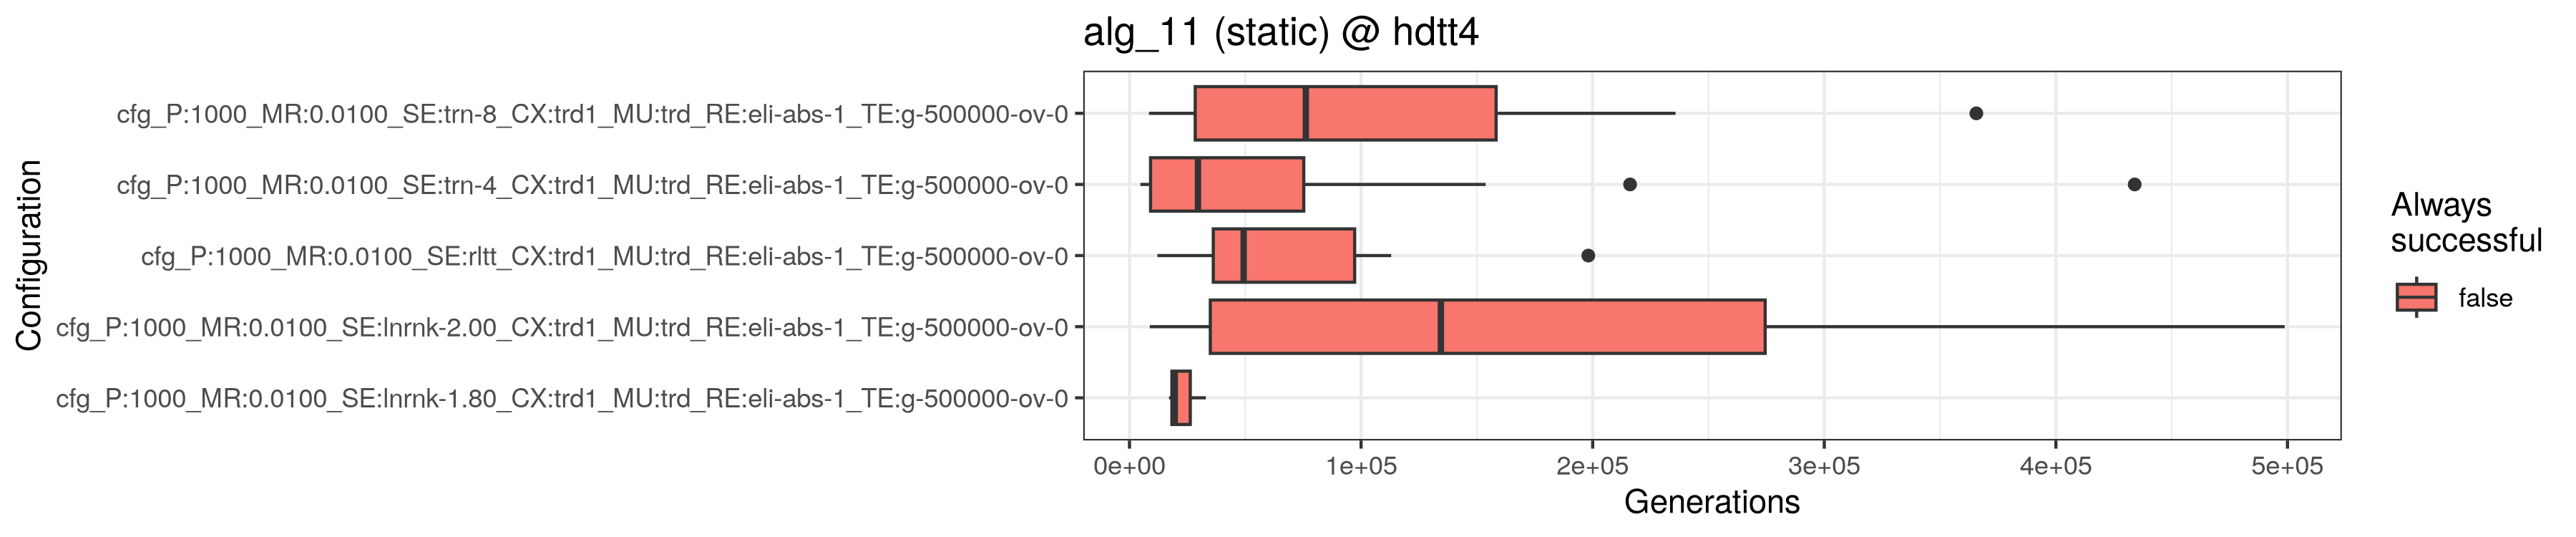
\includegraphics[width=1.28\textwidth]{
            assets/chap-6/generations-taken/hdtt4/alg_11/static_generations_taken.png
        }
        \caption{
            Generations taken on successful runs of \texttt{alg\_11} without
            dynamics on \textit{hdtt4} instances.
        }
        \label{fig:alg_11_static_hdtt4_generations_taken}
    \end{adjustwidth}
\end{figure}

\begin{figure}[h]
    \begin{adjustwidth}{-3cm}{-3cm}
        \centering
        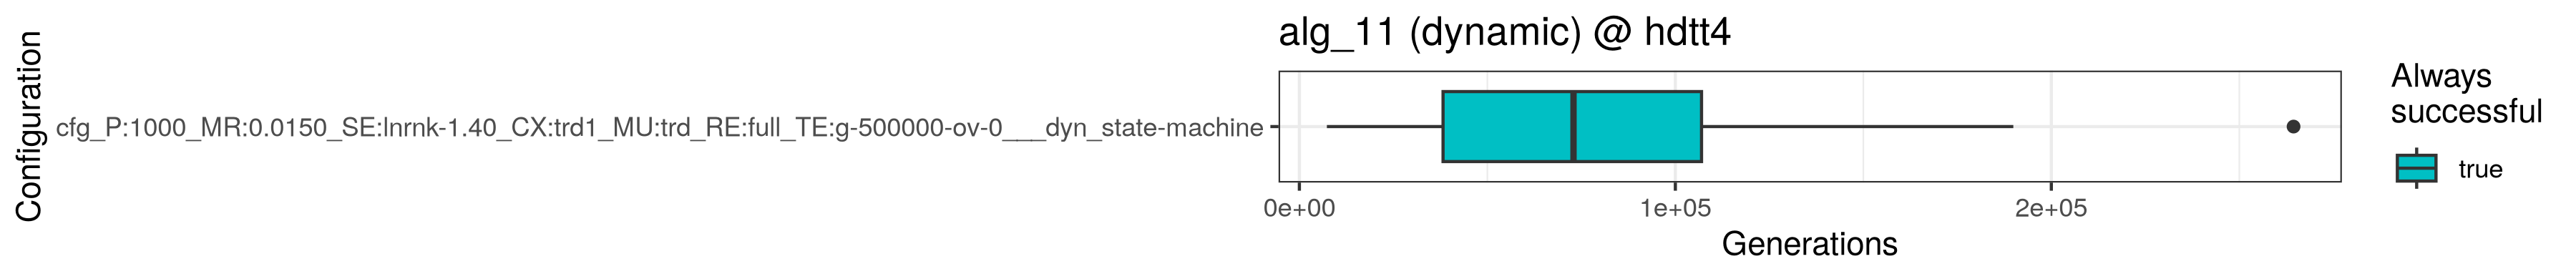
\includegraphics[width=1.28\textwidth]{
            assets/chap-6/generations-taken/hdtt4/alg_11/dynamic_generations_taken.png
        }
        \caption{
            Generations taken on successful runs of \texttt{alg\_11} with
            dynamics on \textit{hdtt4} instances.
        }
        \label{fig:alg_11_dynamic_hdtt4_generations_taken}
    \end{adjustwidth}
\end{figure}

The indirectly encoded algorithm \texttt{alg\_12}, on the other hand, does not
yield such a correlation -- in contrary, for both -- the static and dynamic --
configuration variants the configurations with a 100\% success rate also
correspond to the top performing configurations regarding the amount of
generations taken for finding valid timetables (figures
\ref{fig:alg_12_static_hdtt4_generations_taken} and
\ref{fig:alg_12_dynamic_hdtt4_generations_taken}).
%
\begin{figure}[h!]
    \begin{adjustwidth}{-3cm}{-3cm}
        \centering
        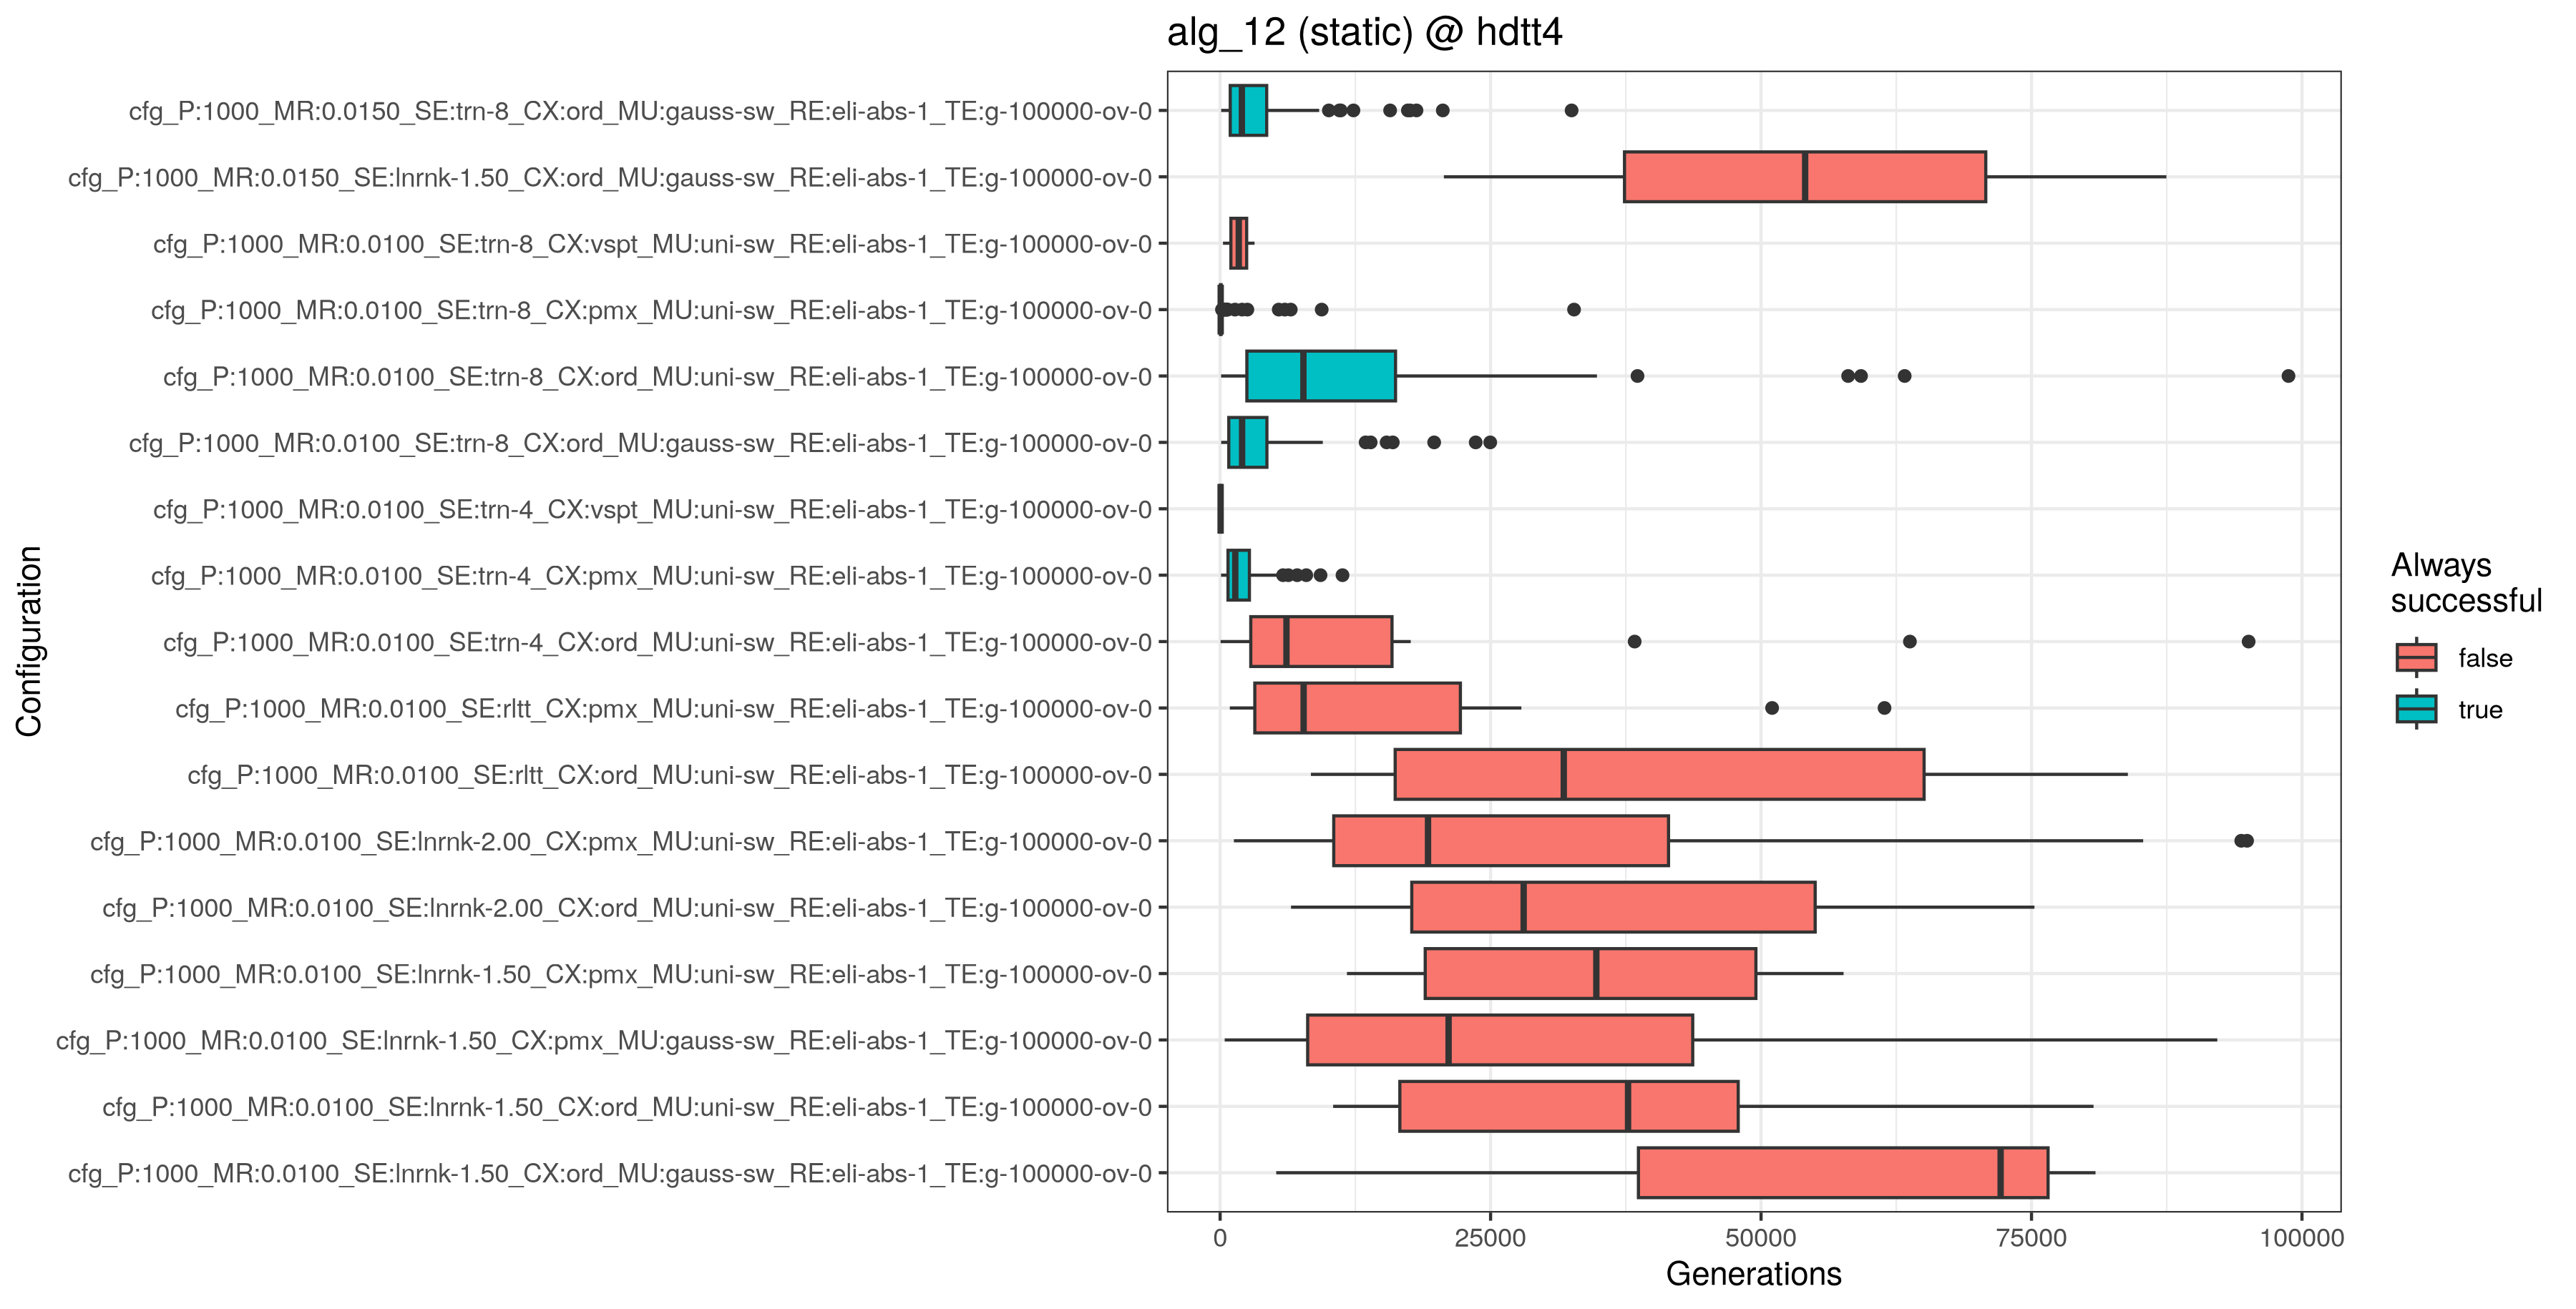
\includegraphics[width=1.28\textwidth]{
            assets/chap-6/generations-taken/hdtt4/alg_12/static_generations_taken.png
        }
        \caption{
            Generations taken on successful runs of \texttt{alg\_12} without
            dynamics on \textit{hdtt4} instances.
        }
        \label{fig:alg_12_static_hdtt4_generations_taken}
    \end{adjustwidth}
\end{figure}
%
\begin{figure}[h!]
    \begin{adjustwidth}{-3cm}{-3cm}
        \centering
        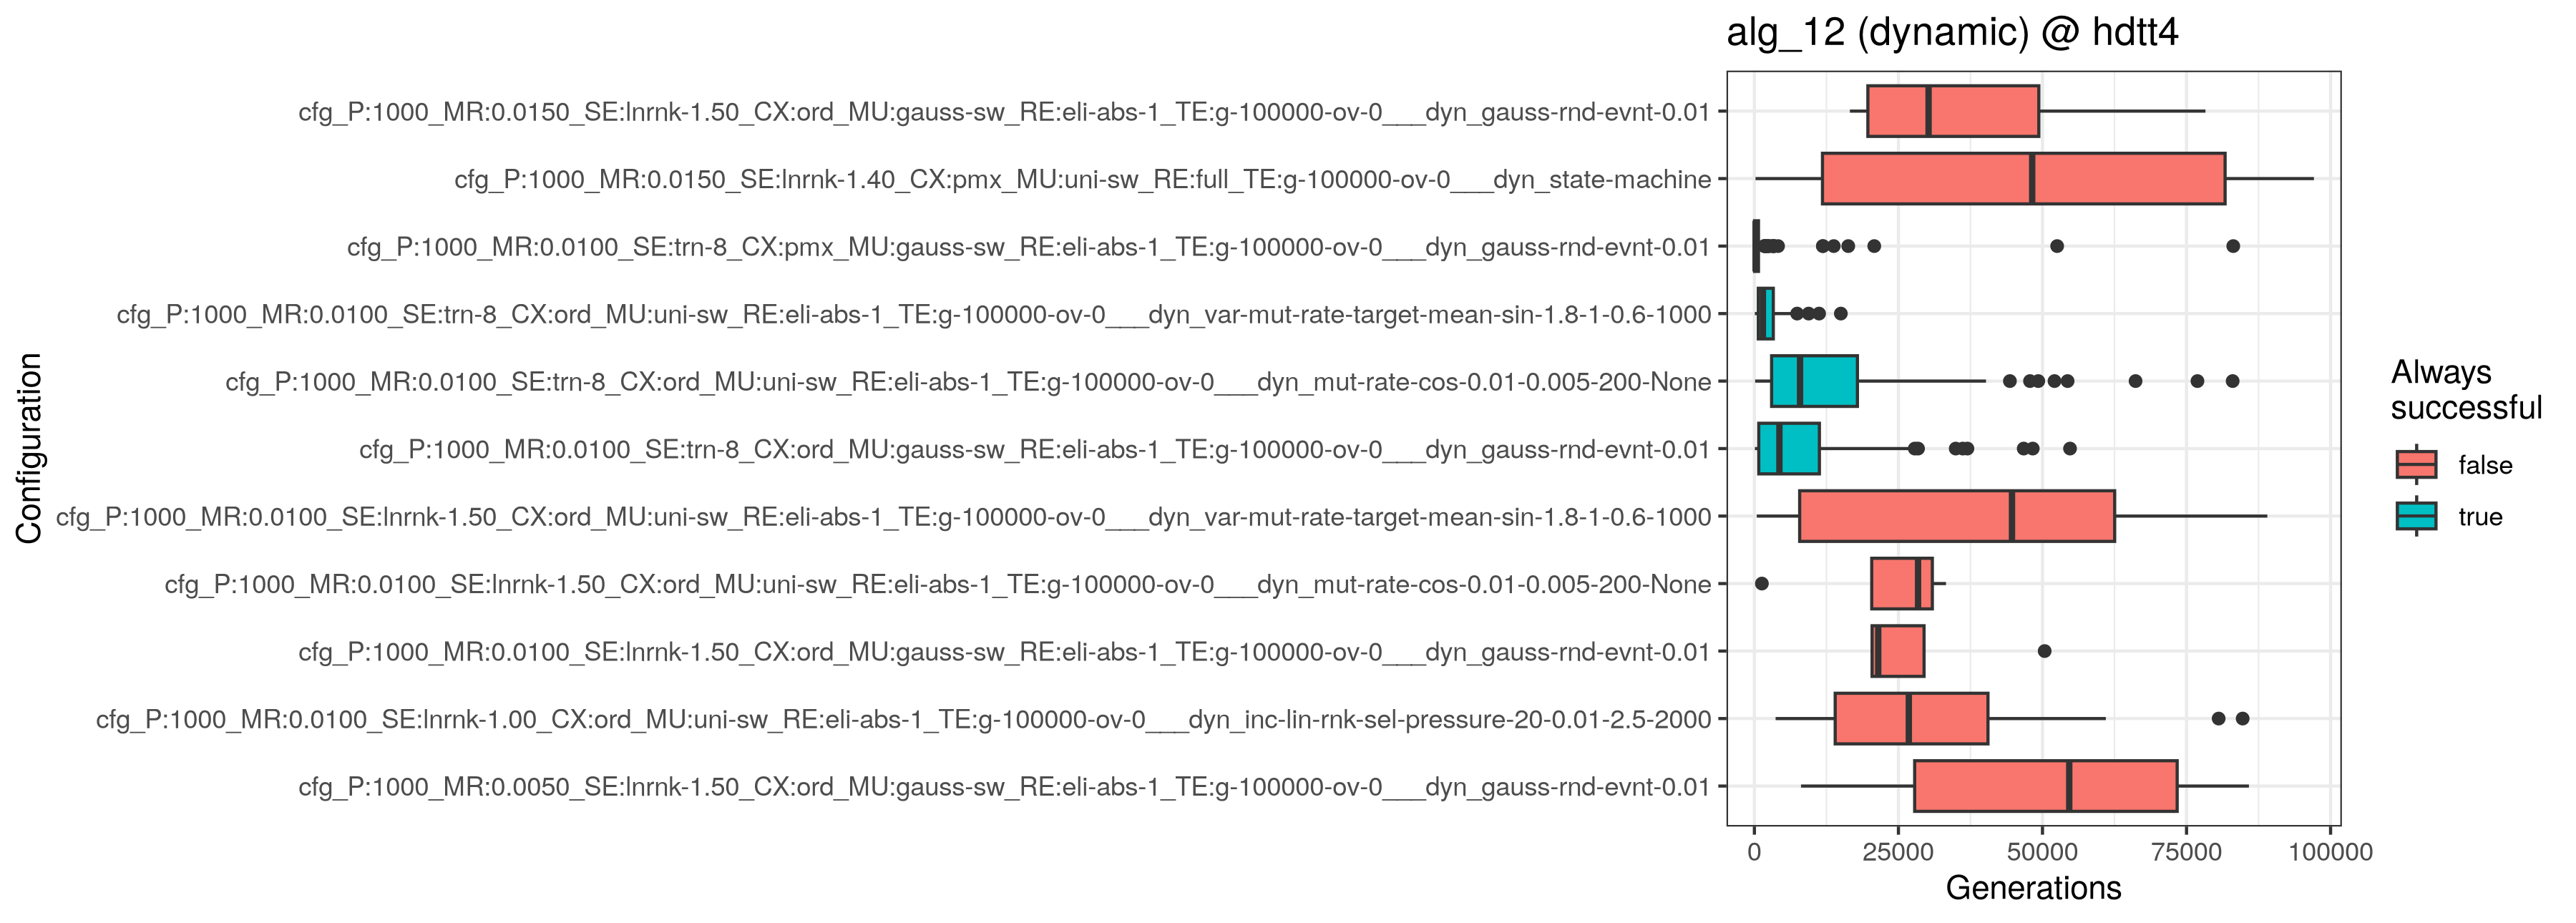
\includegraphics[width=1.28\textwidth]{
            assets/chap-6/generations-taken/hdtt4/alg_12/dynamic_generations_taken.png
        }
        \caption{
            Generations taken on successful runs of \texttt{alg\_12} with
            dynamics on \textit{hdtt4} instances.
        }
        \label{fig:alg_12_dynamic_hdtt4_generations_taken}
    \end{adjustwidth}
\end{figure}

These positive results in favor of the self-parameterized indirect encoding
turn around when trying to solve the \textit{hdtt5} instance.
Not only are the self-parameterized configurations not as reliable as the
tested static configuration, it also takes them a significant amount of
generations more to succeed at this problem instance, than their static
counterparts (figures \ref{fig:alg_12_static_hdtt5_generations_taken} and
\ref{fig:alg_12_dynamic_hdtt5_generations_taken}).



\begin{figure}[h!]
    \begin{adjustwidth}{-3cm}{-3cm}
        \centering
        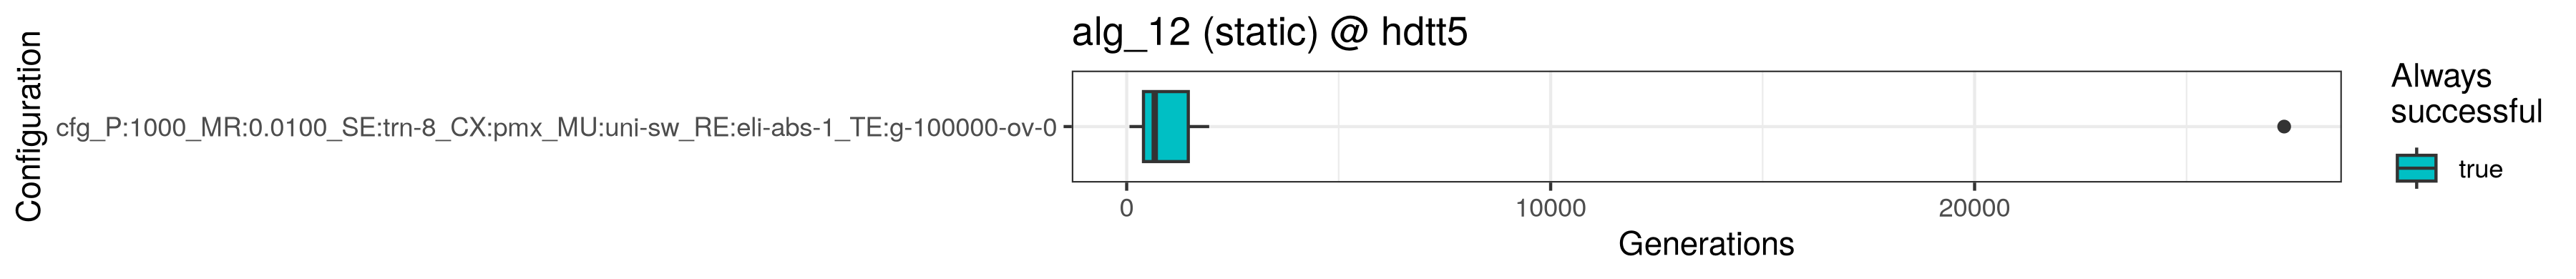
\includegraphics[width=1.28\textwidth]{
            assets/chap-6/generations-taken/hdtt5/alg_12/static_generations_taken.png
        }
        \caption{
            Generations taken on successful runs of \texttt{alg\_12} without
            dynamics on \textit{hdtt5} instances.
        }
        \label{fig:alg_12_static_hdtt5_generations_taken}
    \end{adjustwidth}
\end{figure}

\begin{figure}[h!]
    \begin{adjustwidth}{-3cm}{-3cm}
        \centering
        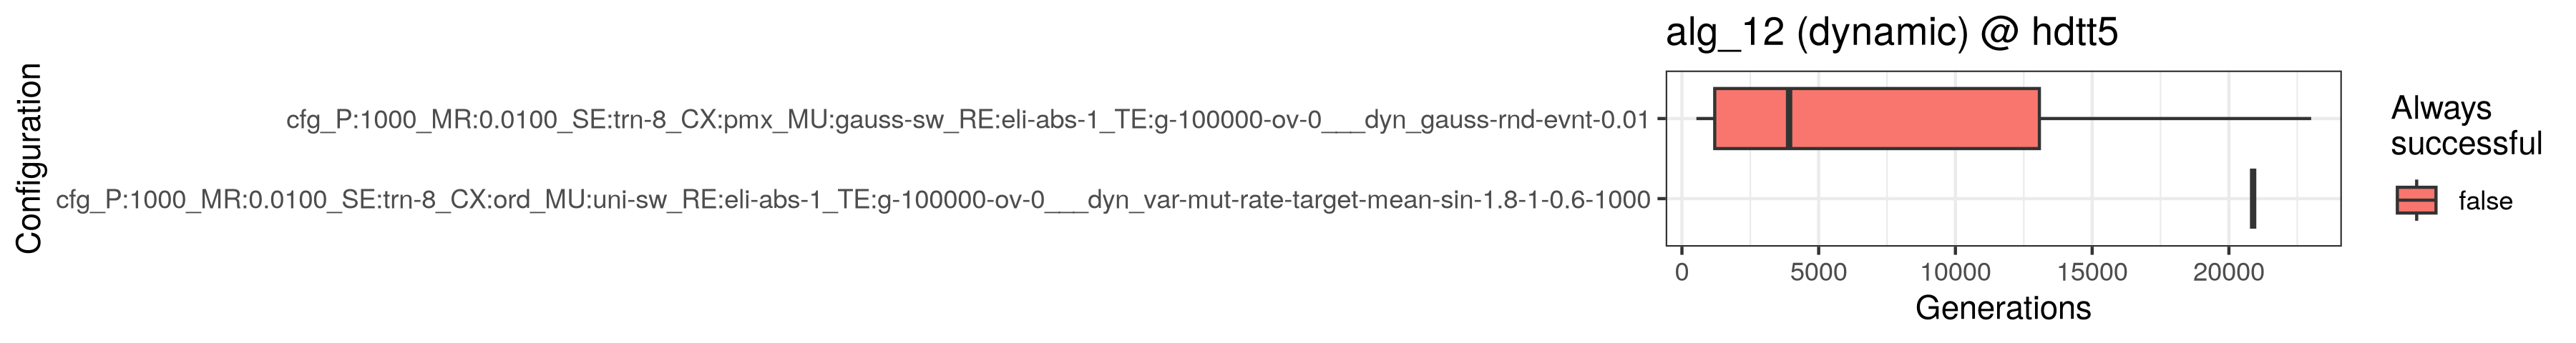
\includegraphics[width=1.28\textwidth]{
            assets/chap-6/generations-taken/hdtt5/alg_12/dynamic_generations_taken.png
        }
        \caption{
            Generations taken on successful runs of \texttt{alg\_12} with
            dynamics on \textit{hdtt5} instances.
        }
        \label{fig:alg_12_dynamic_hdtt5_generations_taken}
    \end{adjustwidth}
\end{figure}
\newpage

%%% Performance %%%%%%%%%%%%%%%%%%%%%%%%%%%%%%%%%%%%%%%%%%%%%%%%%%%%%%%%%%%%%%%%
\section{Performance}
The performance of the algorithms was evaluated based on the number of
generations computed per second. Importantly, self-parameterization techniques
did not introduce significant overhead despite requiring additional computations
on every generation, with both static and dynamic configurations achieving
comparable throughput, especially when their success rates are similar.
This finding underscores that while self-parameterization may affect success
rates or required generations, it does not compromise the computational
efficiency of the algorithms.

It is important to note, that all presented throughput numbers seen in figures
\ref{fig:alg_11_static_hdtt4_gen_per_sec},
\ref{fig:alg_11_dynamic_hdtt4_gen_per_sec},
\ref{fig:alg_12_static_hdtt4_gen_per_sec},
\ref{fig:alg_12_dynamic_hdtt4_gen_per_sec},
\ref{fig:alg_12_static_hdtt5_gen_per_sec} and
\ref{fig:alg_12_dynamic_hdtt5_gen_per_sec}
are highly dependent on the hardware used to execute the algorithms.
All experiments were conducted on an Intel Ultra 9 185H processor and
\SI{64}{\giga\byte} of memory, where the limiting factor was the processors
performance and not the available memory, as the memory usage of the algorithms
never exceeded \SI{50}{\mega\byte}.

\begin{figure}[h]
    \begin{adjustwidth}{-3cm}{-3cm}
        \centering
        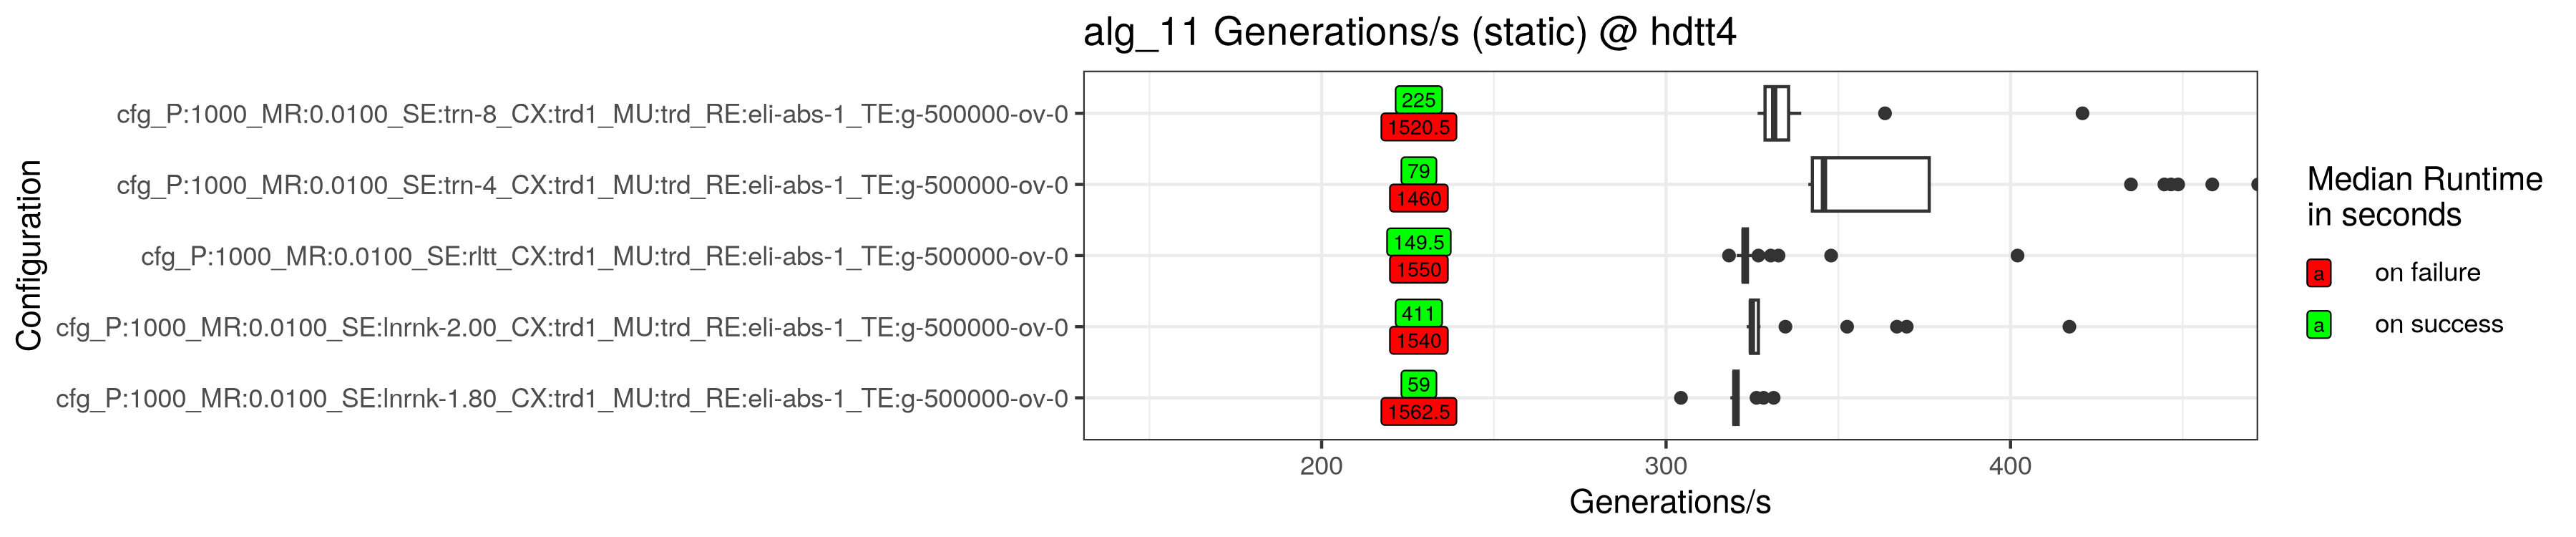
\includegraphics[width=1.28\textwidth]{
            assets/chap-6/performance/hdtt4/alg_11/static_gen_per_sec.png
        }
        \caption{
            Generations per second of \texttt{alg\_11} without
            dynamics on \textit{hdtt4} instances.
        }
        \label{fig:alg_11_static_hdtt4_gen_per_sec}
    \end{adjustwidth}
\end{figure}

\begin{figure}[h]
    \begin{adjustwidth}{-3cm}{-3cm}
        \centering
        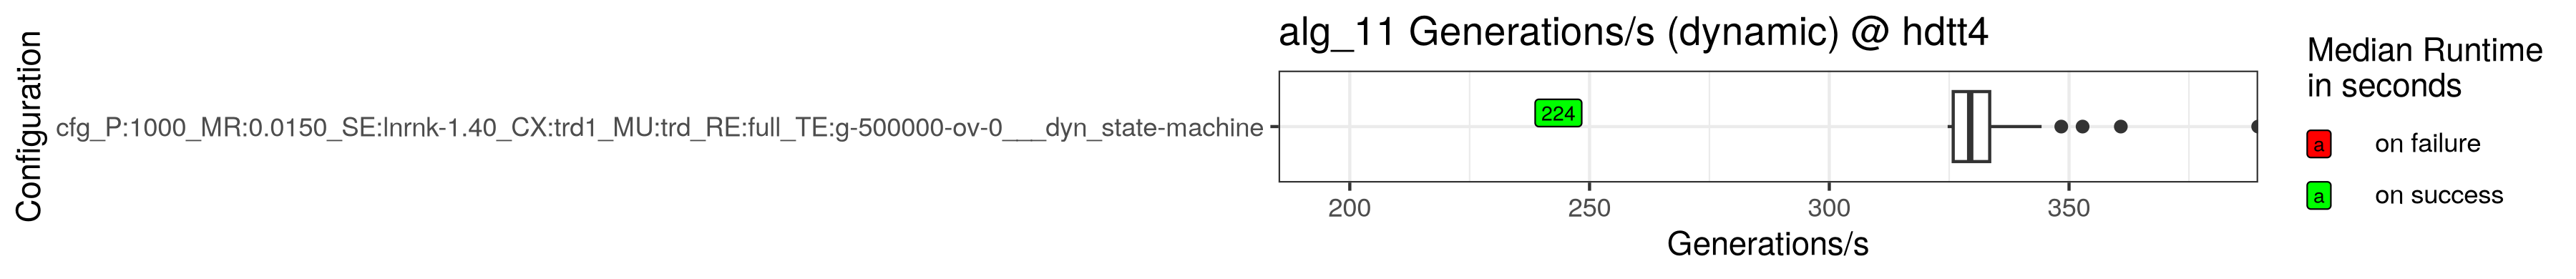
\includegraphics[width=1.28\textwidth]{
            assets/chap-6/performance/hdtt4/alg_11/dynamic_gen_per_sec.png
        }
        \caption{
            Generations per second of \texttt{alg\_11} with
            dynamics on \textit{hdtt4} instances.
        }
        \label{fig:alg_11_dynamic_hdtt4_gen_per_sec}
    \end{adjustwidth}
\end{figure}



\begin{figure}[h!]
    \begin{adjustwidth}{-3cm}{-3cm}
        \centering
        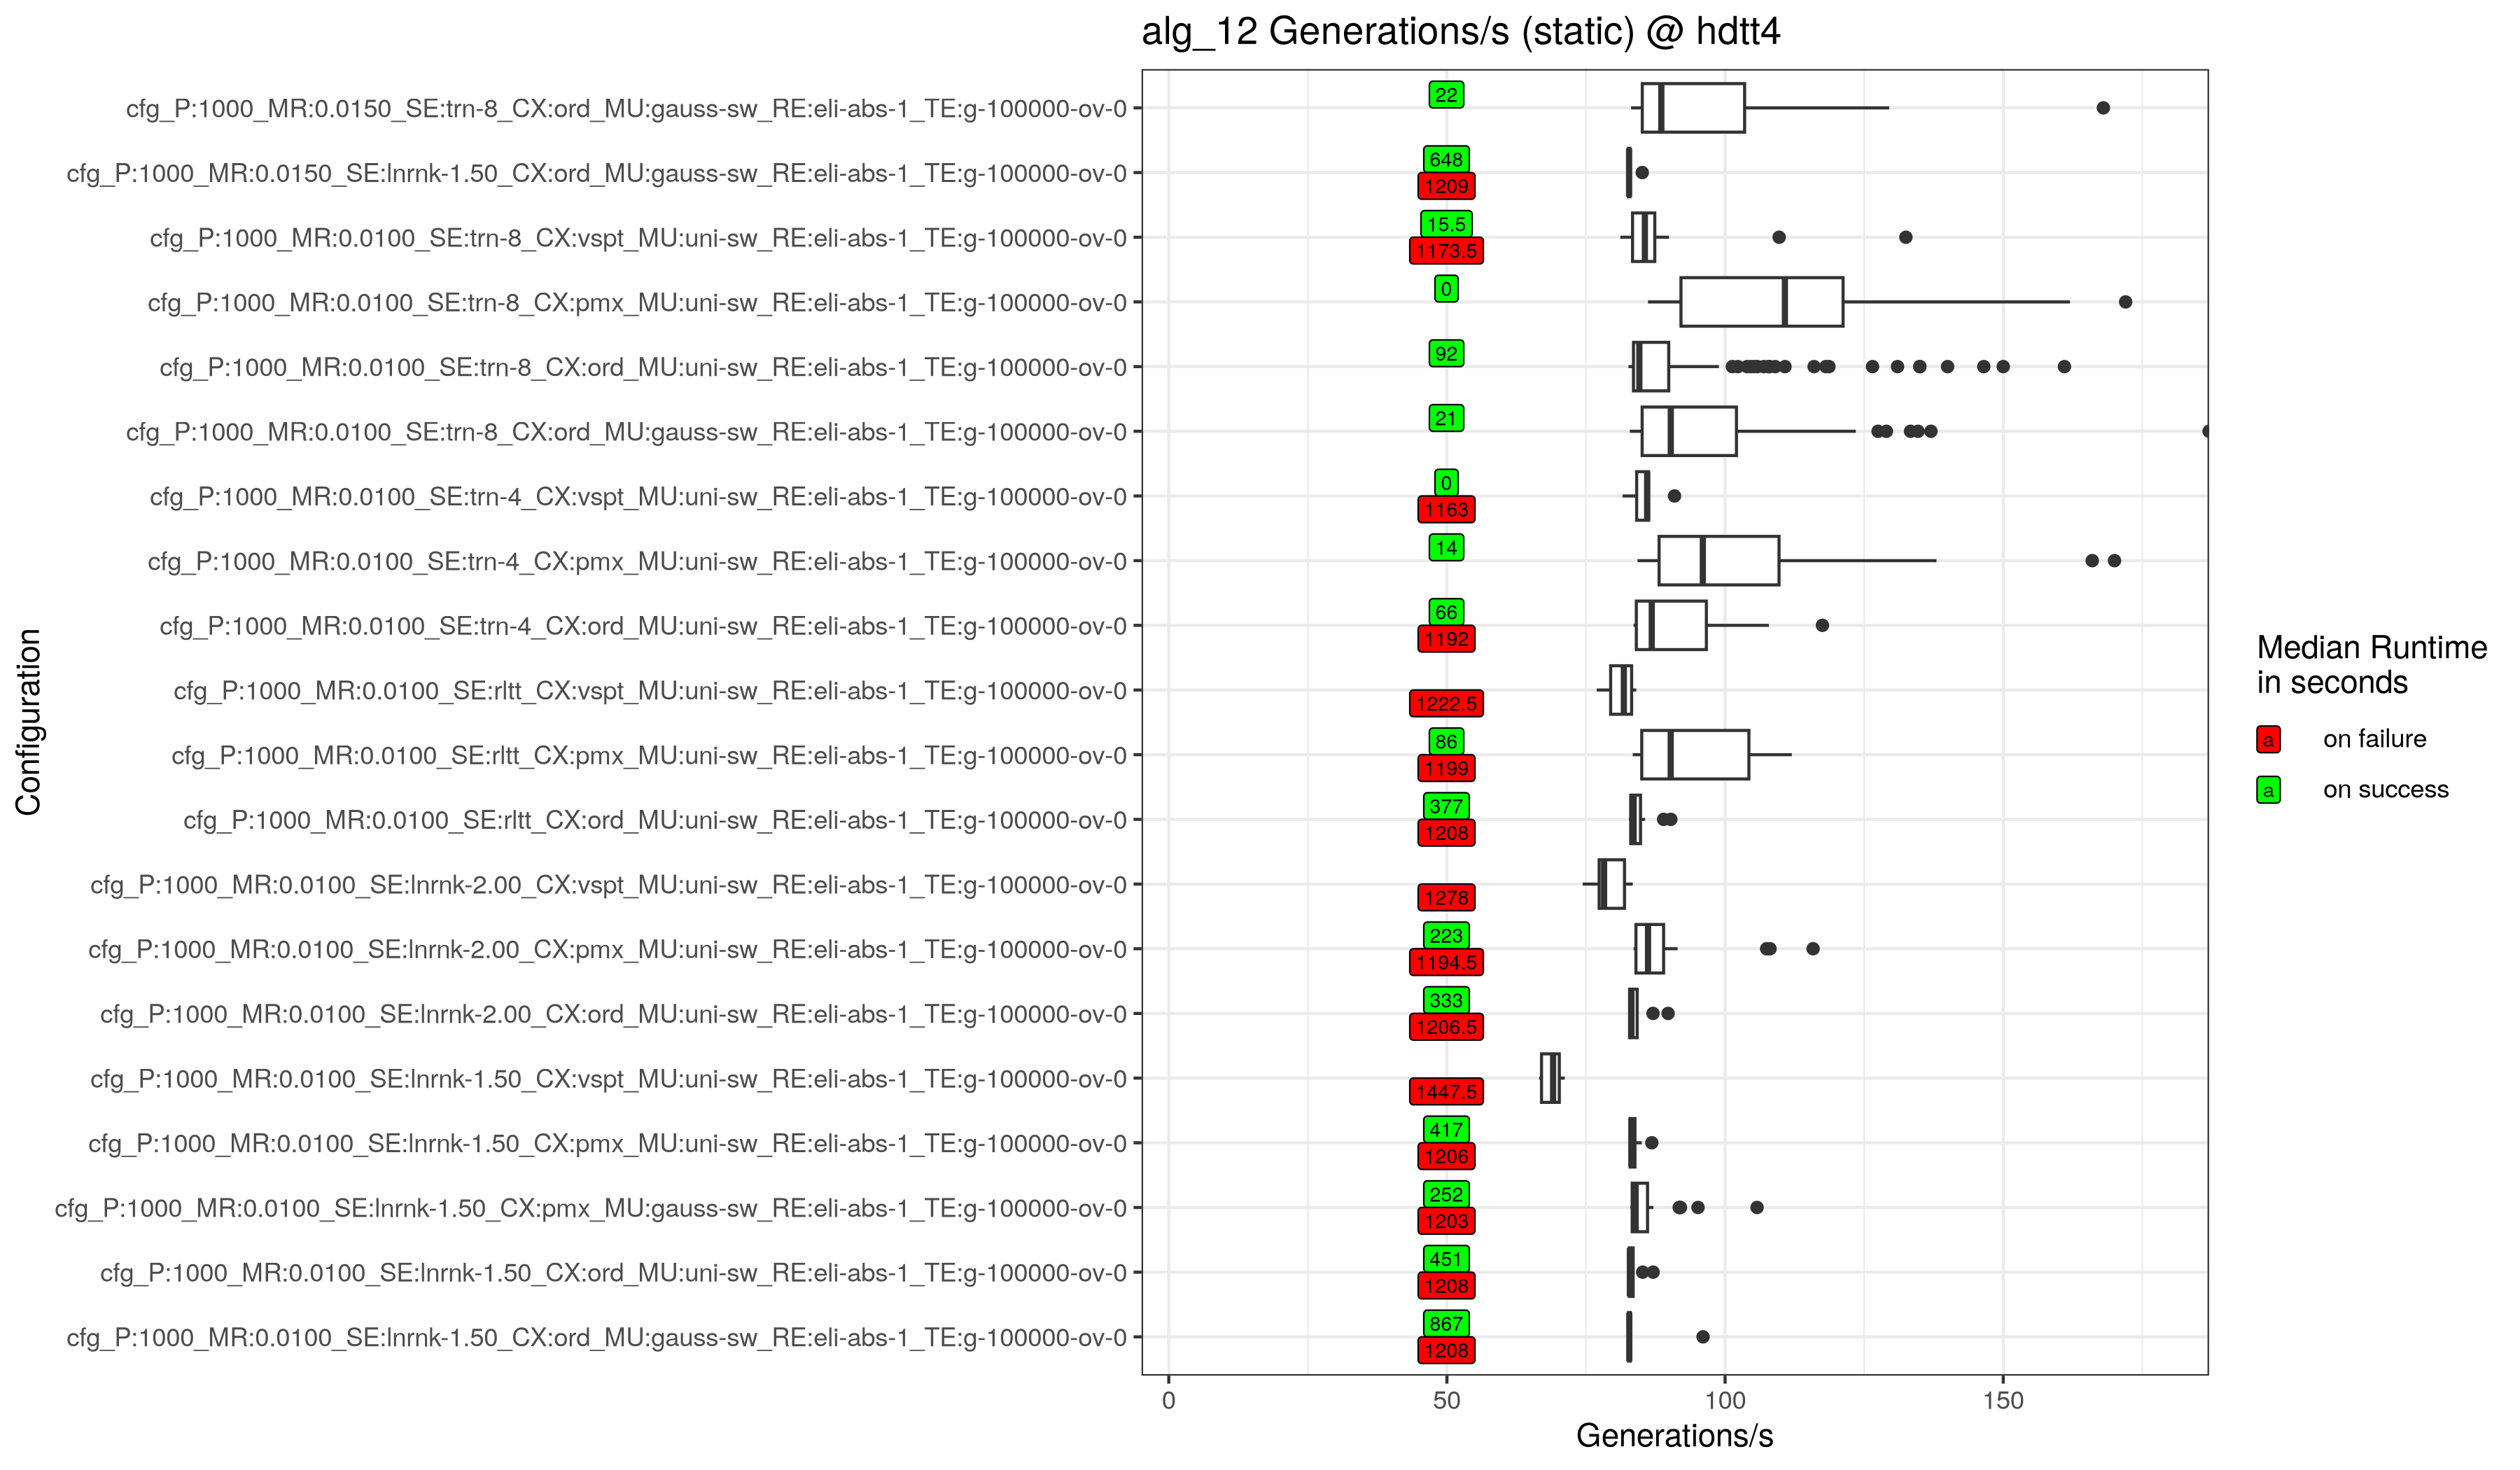
\includegraphics[width=1.28\textwidth]{
            assets/chap-6/performance/hdtt4/alg_12/static_gen_per_sec.png
        }
        \caption{
            Generations per second of \texttt{alg\_12} without
            dynamics on \textit{hdtt4} instances.
        }
        \label{fig:alg_12_static_hdtt4_gen_per_sec}
    \end{adjustwidth}
\end{figure}

\begin{figure}[h!]
    \begin{adjustwidth}{-3cm}{-3cm}
        \centering
        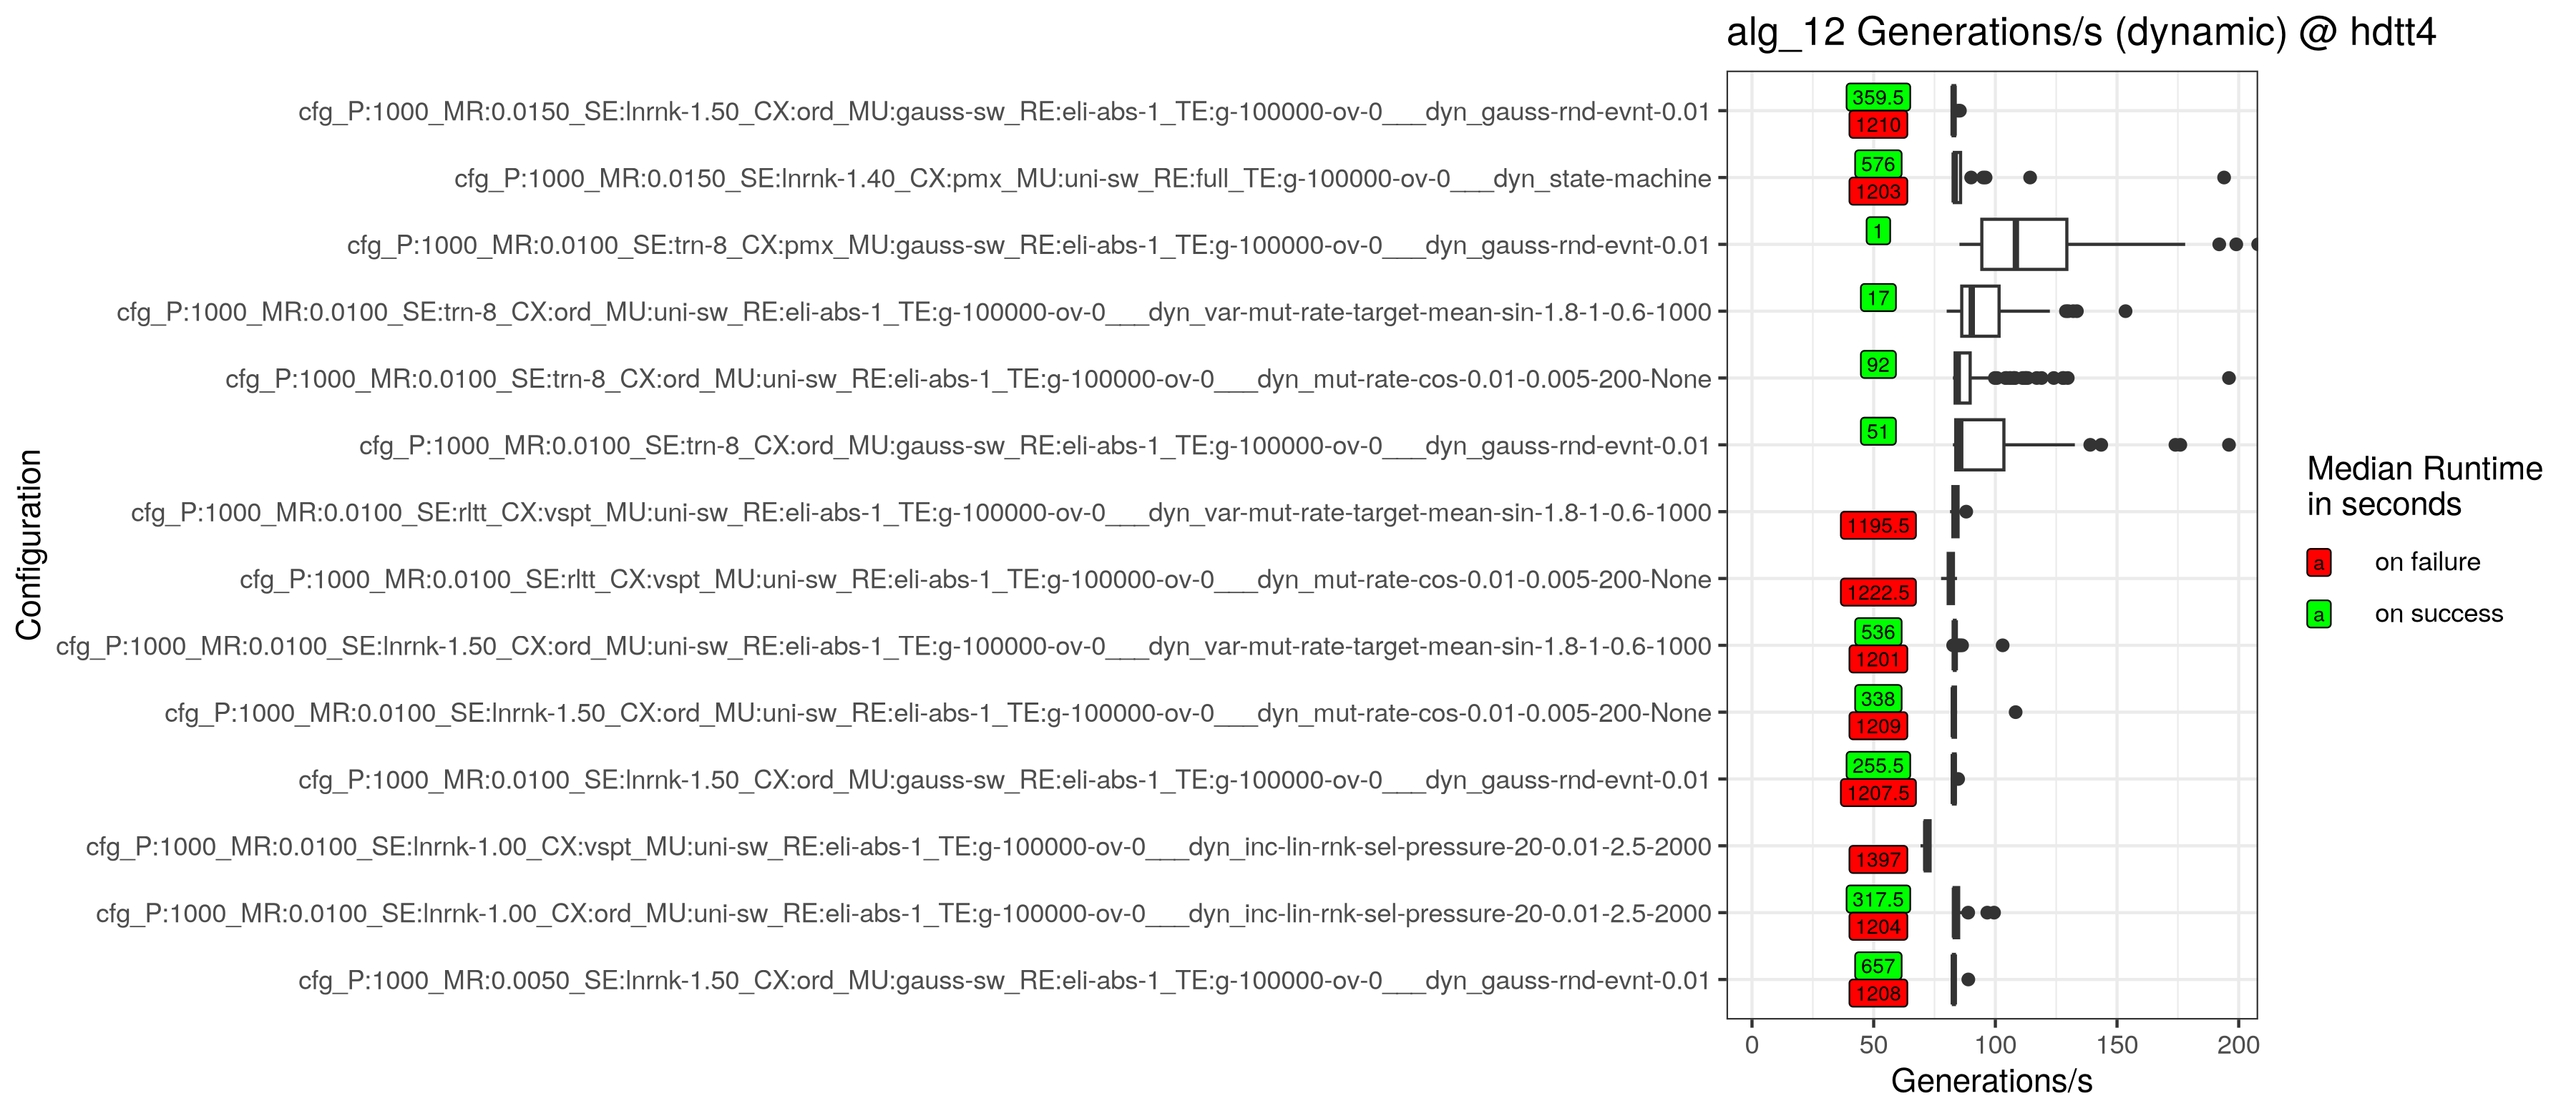
\includegraphics[width=1.28\textwidth]{
            assets/chap-6/performance/hdtt4/alg_12/dynamic_gen_per_sec.png
        }
        \caption{
            Generations per second of \texttt{alg\_12} with
            dynamics on \textit{hdtt4} instances.
        }
        \label{fig:alg_12_dynamic_hdtt4_gen_per_sec}
    \end{adjustwidth}
\end{figure}



\begin{figure}[h!]
    \begin{adjustwidth}{-3cm}{-3cm}
        \centering
        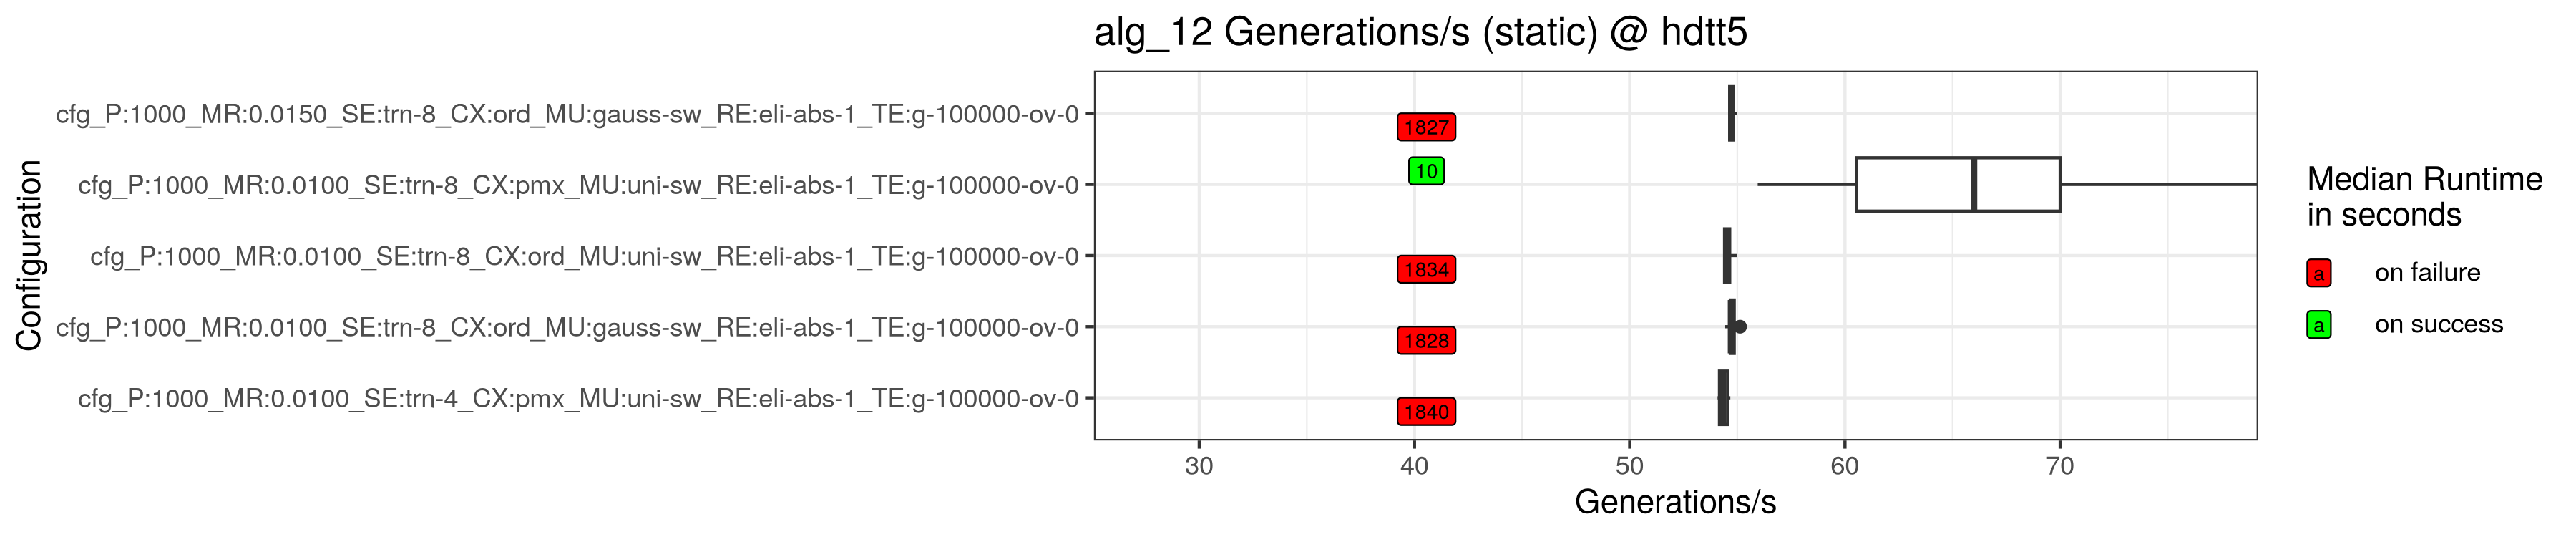
\includegraphics[width=1.28\textwidth]{
            assets/chap-6/performance/hdtt5/alg_12/static_gen_per_sec.png
        }
        \caption{
            Generations per second of \texttt{alg\_12} without
            dynamics on \textit{hdtt5} instances.
        }
        \label{fig:alg_12_static_hdtt5_gen_per_sec}
    \end{adjustwidth}
\end{figure}

\begin{figure}[h!]
    \begin{adjustwidth}{-3cm}{-3cm}
        \centering
        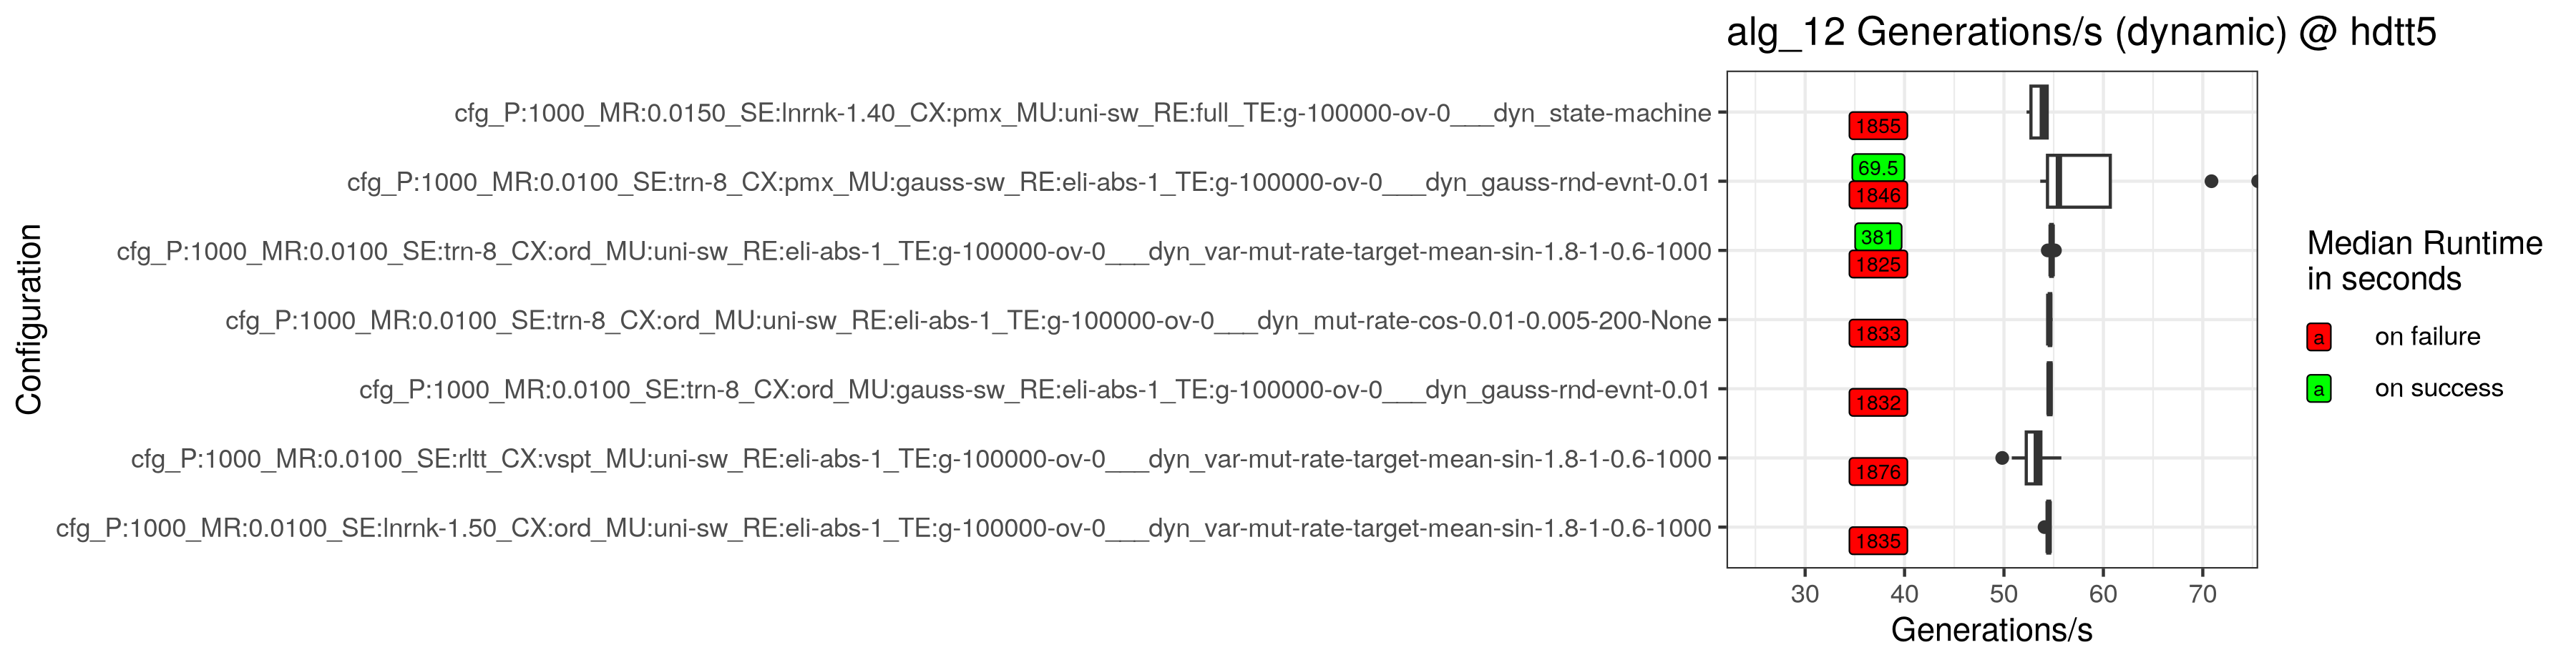
\includegraphics[width=1.28\textwidth]{
            assets/chap-6/performance/hdtt5/alg_12/dynamic_gen_per_sec.png
        }
        \caption{
            Generations per second of \texttt{alg\_12} with
            dynamics on \textit{hdtt5} instances.
        }
        \label{fig:alg_12_dynamic_hdtt5_gen_per_sec}
    \end{adjustwidth}
\end{figure}


%%%%%%%%%%%%%%%%%%%%%%%%%%%%%%%%%%%%%%%%%%%%%%%%%%%%%%%%%%%%%%%%%%%%%%%%%%%%%%%%
%%% 7. Discussion                                                            %%%
%%%%%%%%%%%%%%%%%%%%%%%%%%%%%%%%%%%%%%%%%%%%%%%%%%%%%%%%%%%%%%%%%%%%%%%%%%%%%%%%
\chapter{Discussion}
This chapter provides a detailed discussion of the previously presented results,
with a particular focus on analyzing the impact of self-parameterization on
the genetic algorithms' reliability and performance. To facilitate this
analysis, visualizations of selected algorithm executions are presented in the
form of diagrams. Each diagram follows a consistent structure: the
$x$-axis represents the number of generations, while the primary $y$-axis on
the left displays the recorded metrics in terms of the objective value.
These metrics include the objective values of the \textit{best}, \textit{mean},
\textit{median} and \textit{worst} individual of the respective generation.
The secondary $y$-axis on the right shows the scale for the diversity metric.

The diversity metric plays a crucial role in evaluating the population's
variation throughout the evolutionary process. High diversity typically
indicates that the population explores a broader range of solutions, which
helps prevent premature convergence. Conversely, low diversity may signal
stagnation and a tendency to converge around local maxima. In this study,
diversity is quantified using the \textit{normalized Shannon entropy}.

Shannon entropy, originally introduced in information theory, measures the
uncertainty or randomness in a set of values \cite{shannon1948mathematical}.
For a population of $N$ individuals, where $p_i$ represents the probability of
a specific objective value $i$, the Shannon entropy $H$ is calculated as:
\begin{equation}
    H = - \sum_{i=1}^{N} p_i \cdot log_2(p_i)
\end{equation}

To ensure a uniform interpretation across different scenarios, the Shannon
entropy is normalized by dividing it by the maximum possible entropy
$H_{max} = log_2(N)$, resulting in a value between $0.0$ and $1.0$.
A diversity value of $0.0$ represents minimal entropy (low diversity), where
all individuals in the population share the same objective value, indicating
stagnation.
In contrast, a value of $1.0$ represents maximum entropy (high diversity),
signifying a uniform distribution of objective values and this high variation
within the population.
%
The normalized Shannon entropy provides a robust and interpretable measure of
diversity, allowing of a clear assessment of the population's exploration
capabilities throughout the evolutionary process.

By comparing static and self-parameterized configurations, this
discussion aims to highlight the benefits and limitations of the
self-parameterization techniques. Furthermore, the analysis examines the role
of different encoding schemes in shaping the behavior and performance of the
genetic algorithms.

%%% Direct Encoding %%%%%%%%%%%%%%%%%%%%%%%%%%%%%%%%%%%%%%%%%%%%%%%%%%%%%%%%%%%%
\section{Direct Encoding}
The results from the previous chapter clearly demonstrate that \texttt{alg\_11}
utilizing the direct encoding scheme, consistently struggles to reliably solve
the \textit{hdtt4} problem instance.
Regardless of which \textit{static} configuration was used, this algorithm was
not able to achieve satisfying success rates, which indicate its limitations in
this context.
In contrast, \texttt{alg\_12}, employing the indirect encoding scheme, achieves
a perfect 100\% success rate with multiple configurations, highlighting its
superior reliability for this problem instance.

To better understand the behavior of \texttt{alg\_11}, figures
\ref{fig:hdtt4_alg11_direct_static_succ_median} and
\ref{fig:hdtt4_alg11_direct_static_fail_median} are particularly insightful.
These diagrams illustrate the metrics of median successful and unsuccessful
runs. The term \enquote{median} here refers to the algorithm's performance in
terms of the number of generations required, providing a representative snapshot
of its typical behavior.
\begin{figure}[h]
    \begin{adjustwidth}{-3cm}{-3cm}
        \centering
        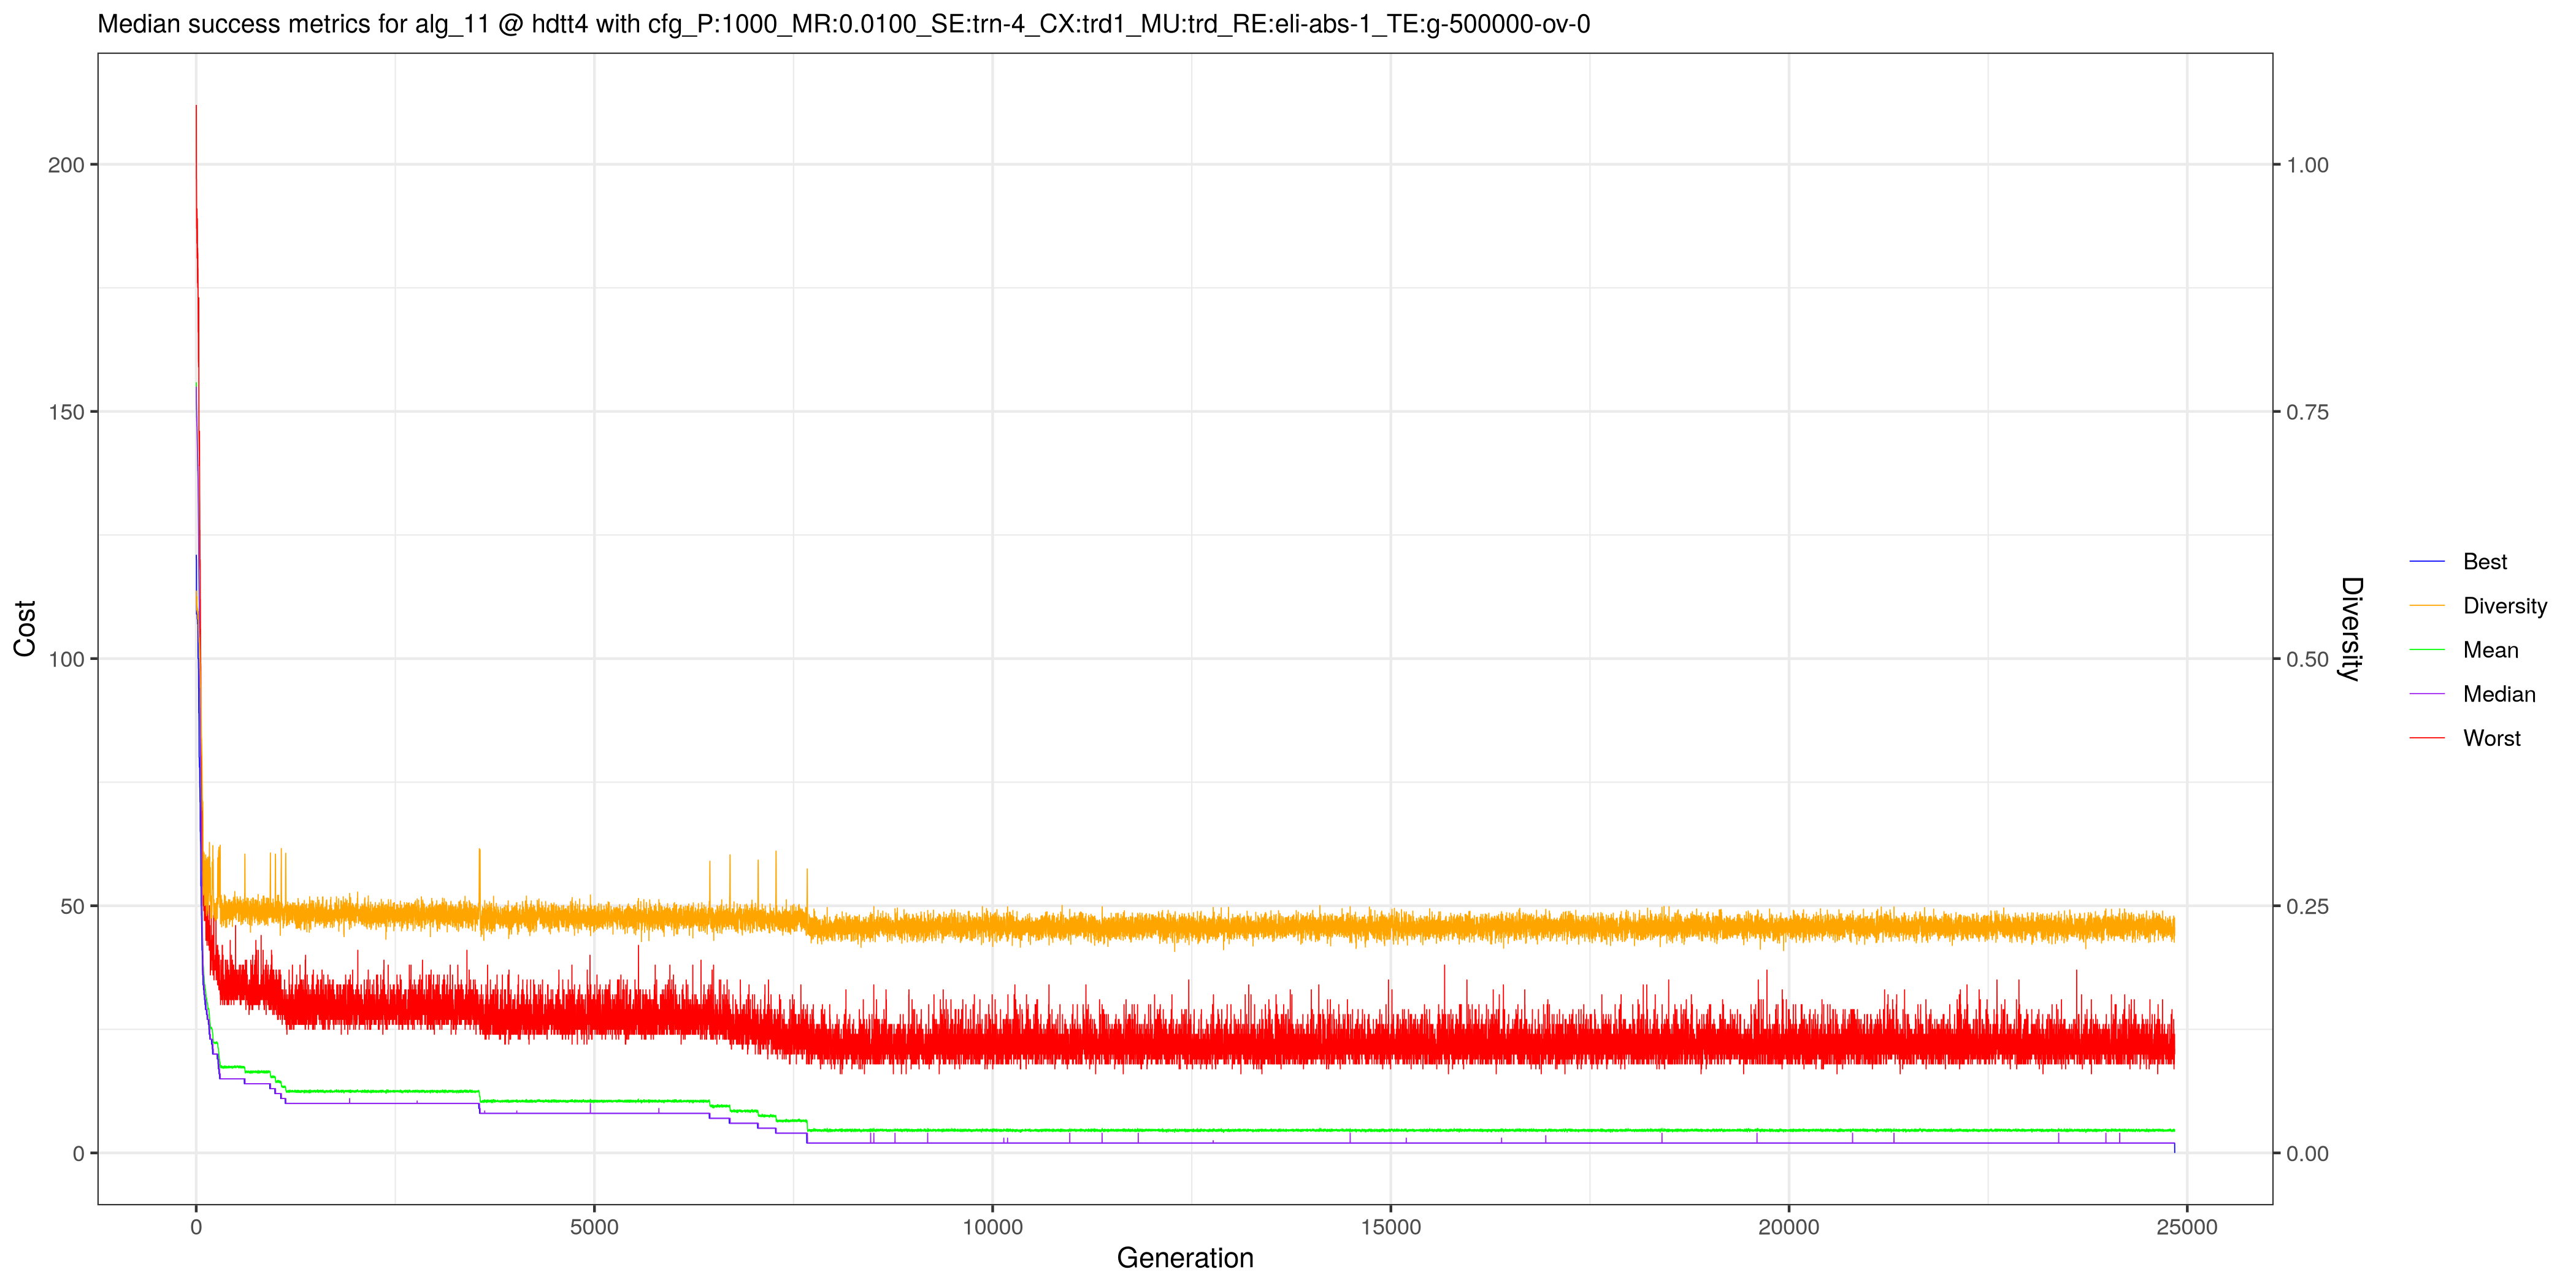
\includegraphics[width=1.28\textwidth]{assets/chap-7/discussion_1/hdtt4/alg_11/direct_static_succ_median.png}
        \caption{
            Runtime metrics of \texttt{alg\_11} during a successful run solving
            \textit{hdtt4}.
        }
        \label{fig:hdtt4_alg11_direct_static_succ_median}
    \end{adjustwidth}
\end{figure}

\begin{figure}[h]
    \begin{adjustwidth}{-3cm}{-3cm}
        \centering
        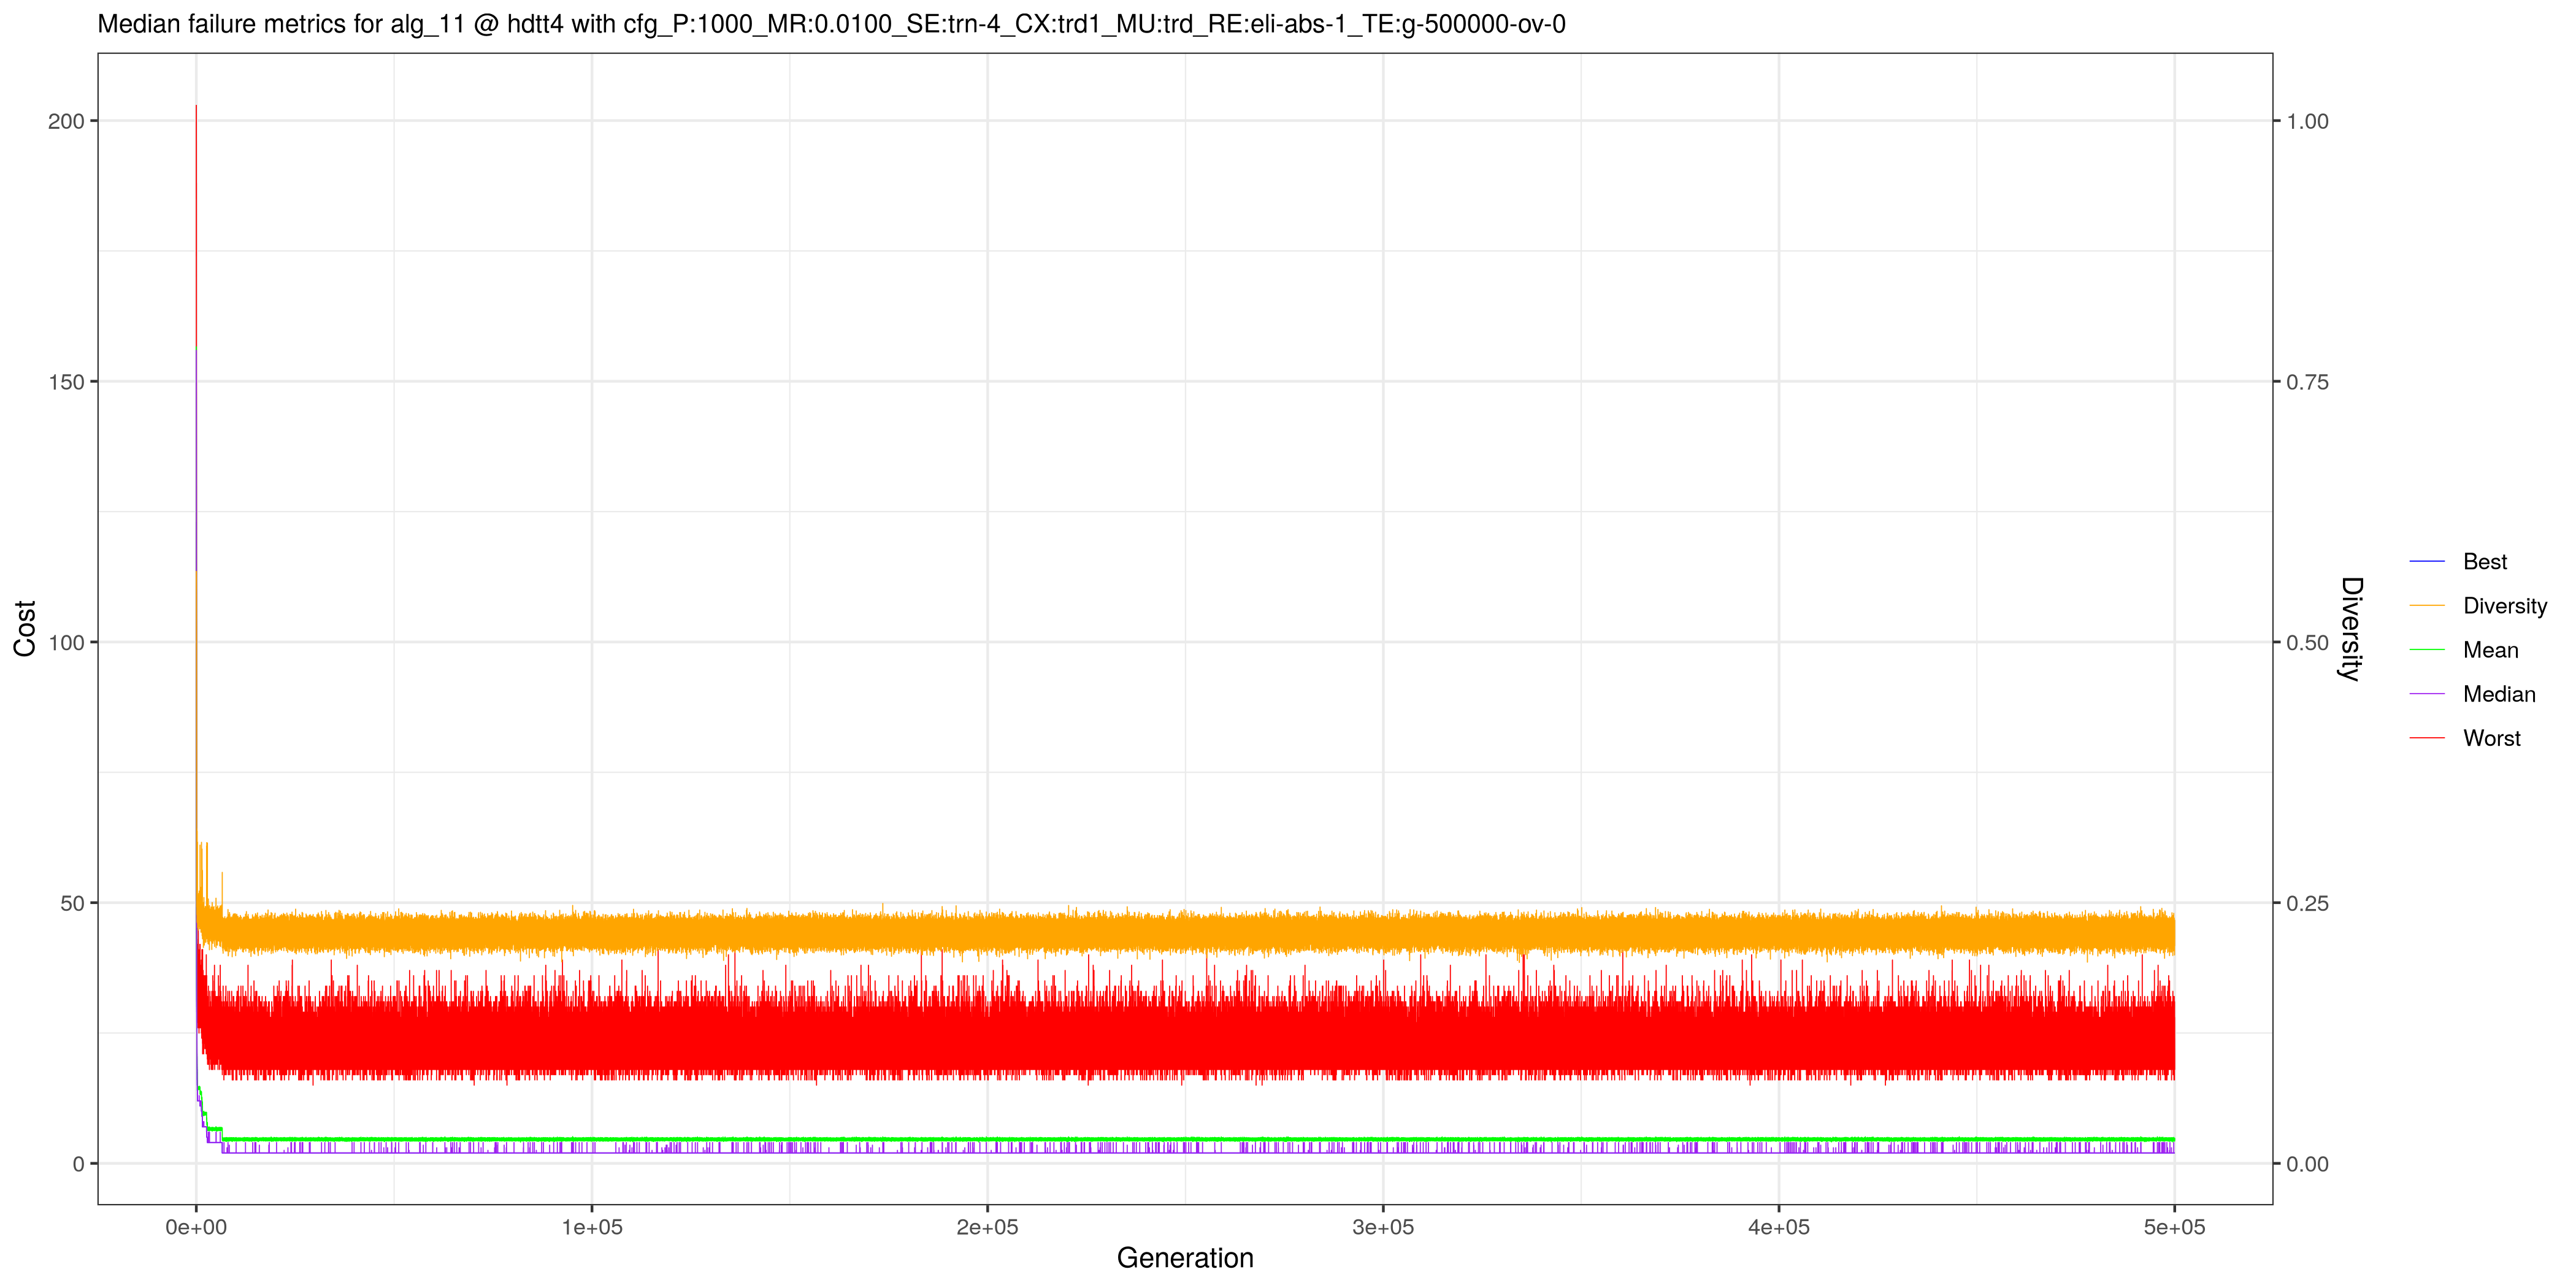
\includegraphics[width=1.28\textwidth]{assets/chap-7/discussion_1/hdtt4/alg_11/direct_static_fail_median.png}
        \caption{
            Runtime metrics of \texttt{alg\_11} during an unsuccessful run
            trying to solve \textit{hdtt4}.
        }
        \label{fig:hdtt4_alg11_direct_static_fail_median}
    \end{adjustwidth}
\end{figure}

\subsection{Static Configuration}
Figure \ref{fig:hdtt4_alg11_direct_static_succ_median} depicts a typical
successful run of \texttt{alg\_11} under static configurations. While it
showcases eventual success, the progression is marked by an absence of notable
changes in population metrics, except when better solutions are discovered.
This lack of variability is particular evident in the diversity metric.
Over the course of the visualized execution, diversity either stagnates or
declines slightly, revealing a significant limitation to static configurations:
their inability to foster continued exploration of the solution space.

Figure \ref{fig:hdtt4_alg11_direct_static_fail_median} further emphasizes this
point by illustrating an unsuccessful run. Here, the population stagnates
entirely, as evidenced by both the flat trajectory of the diversity metric
and the lack of improvement in objective values. This behavior suggests that
once the algorithm becomes stuck in a local maximum, it lacks the mechanisms to
escape.
Without any means to search within the same confined region of the solution
space, ultimately terminating at the generation limit without producing a
feasible timetable solution.

\subsection{Dynamic Configuration (Self-Parameterization)}
\begin{figure}[h]
    \begin{adjustwidth}{-3cm}{-3cm}
        \centering
        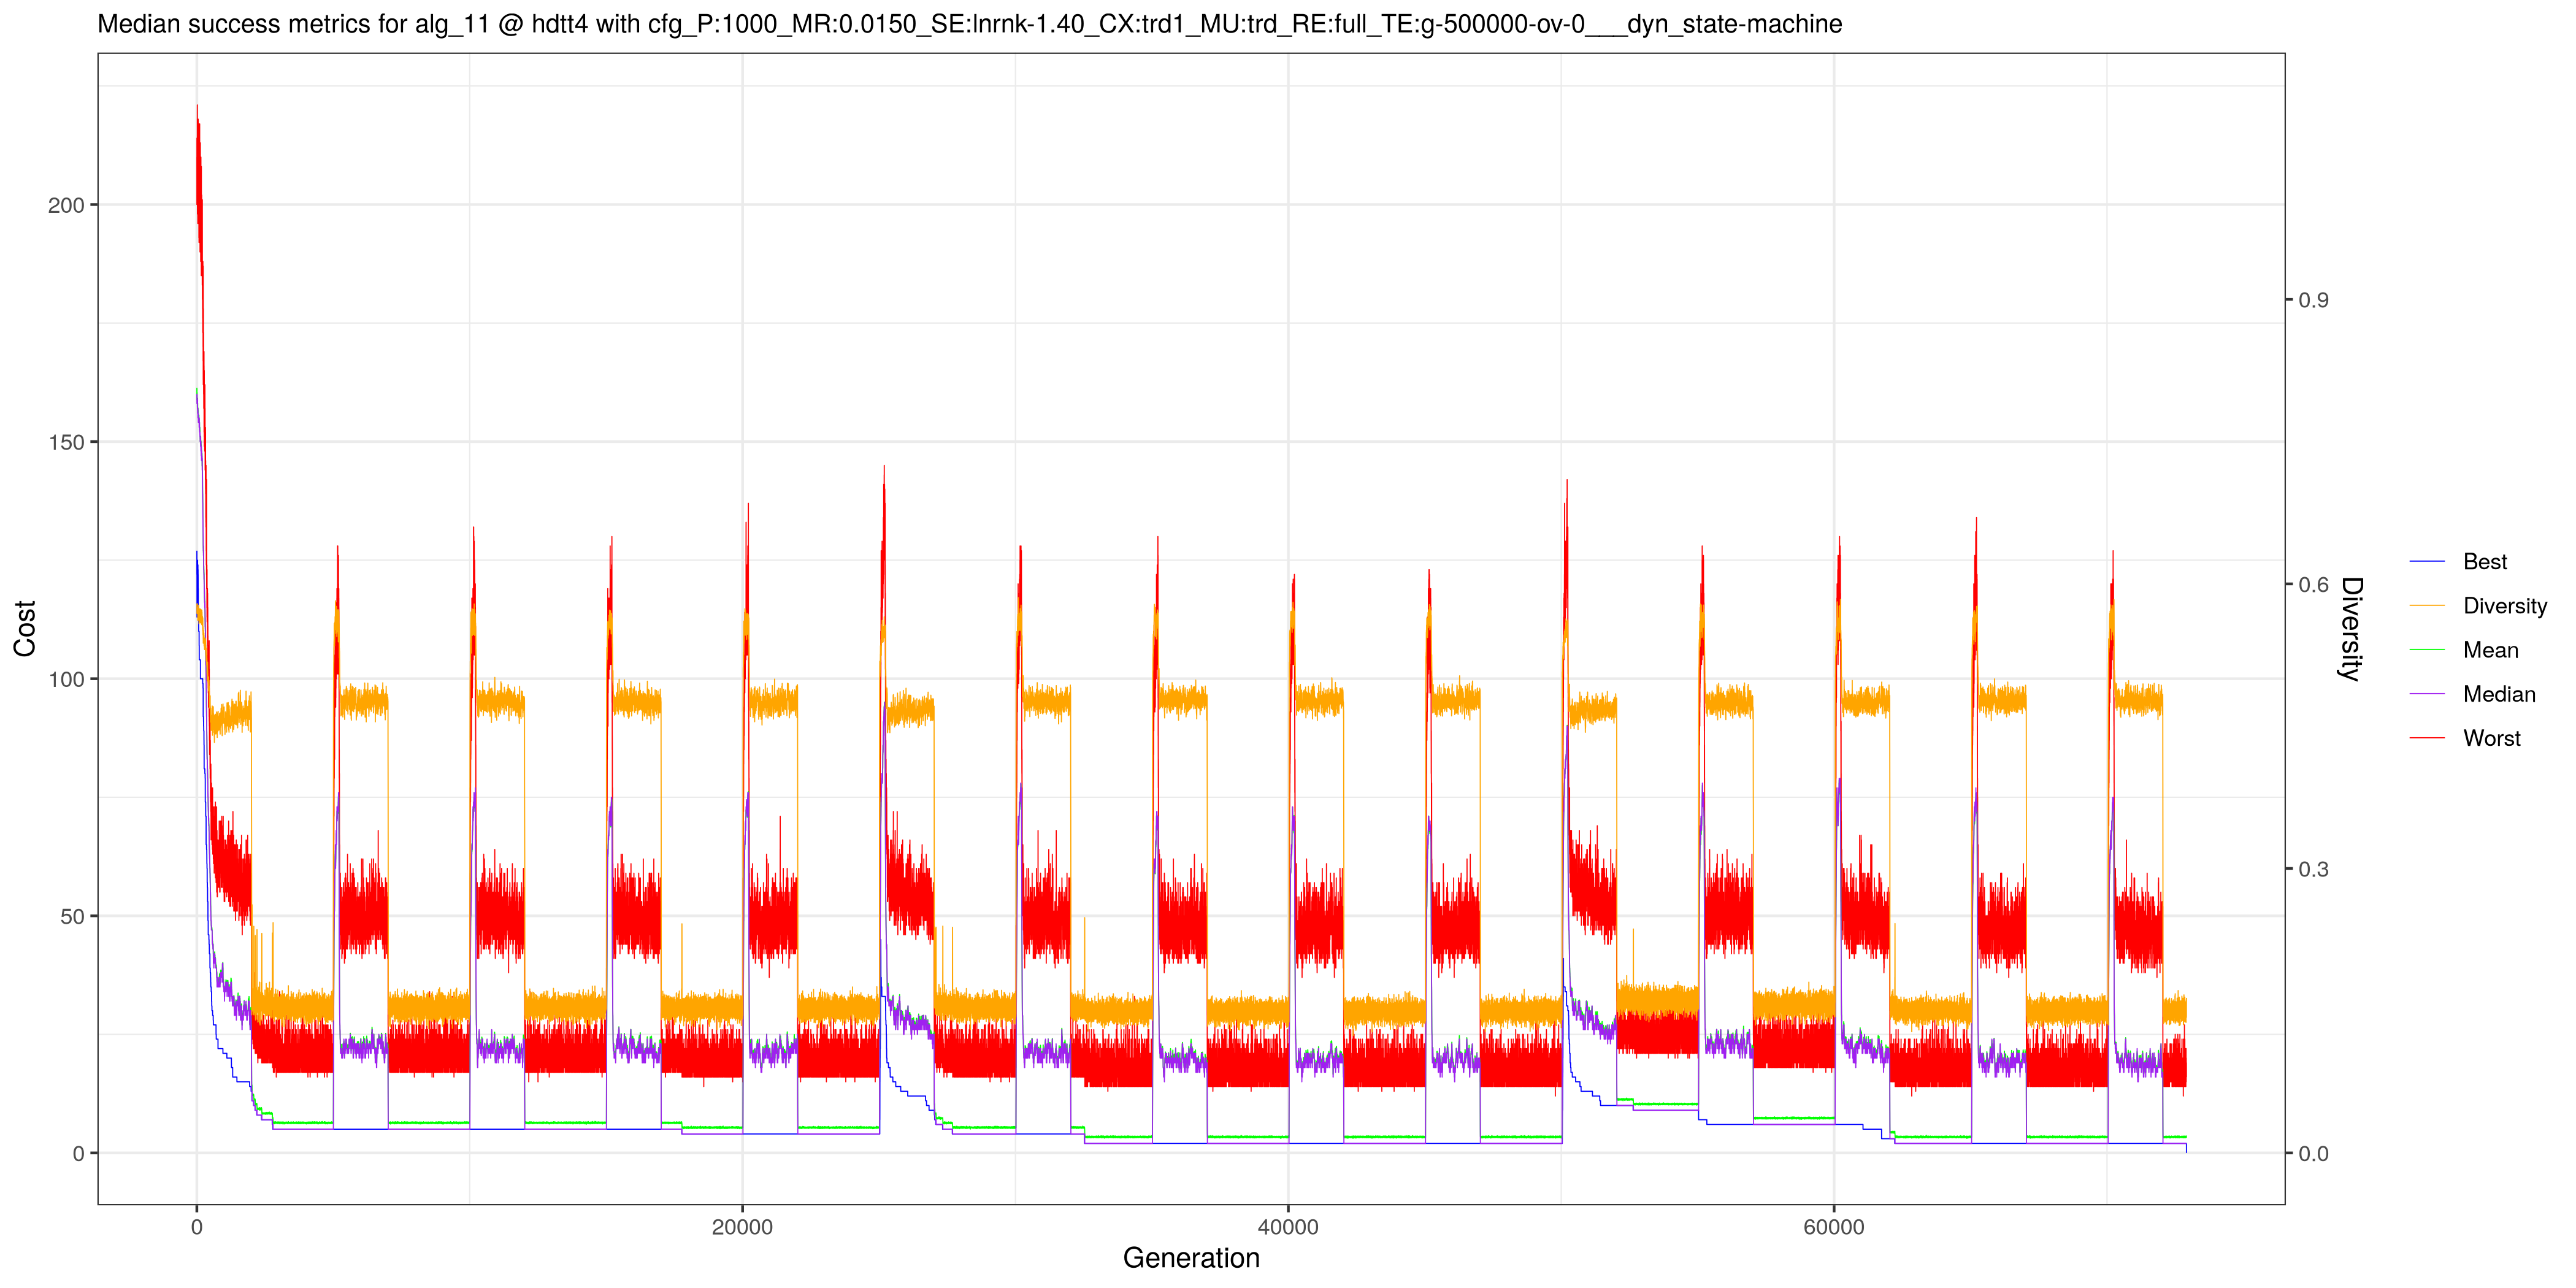
\includegraphics[width=1.28\textwidth]{assets/chap-7/discussion_1/hdtt4/alg_11/direct_dynamic_succ_median.png}
        \caption{
            Runtime metrics of \texttt{alg\_11} with self-parameterization
            during a successful run solving \textit{hdtt4}.
        }
        \label{fig:hdtt4_alg11_direct_dynamic_succ_median}
    \end{adjustwidth}
\end{figure}

Figure \ref{fig:hdtt4_alg11_direct_dynamic_succ_median} offers a compelling
contrast by showcasing a successful run of \texttt{alg\_11} with the
\textit{StateMachine} dynamic applied.
The plot vividly captures the periodic parameter changes introduced by the
self-parameterization technique, highlighting its impact on the algorithm's
behavior.
As described in \ref{StateMachine}, the state machine dynamic cycles through
three distinct parameter states -- broad, focus and finish -- over intervals
of $5000$ generations. These periodic transitions are clearly visible in the
diagram as recurring spikes in both the worst objective value and the
diversity metric.

The state machine dynamic addresses one of the key shortcomings of static
configurations: premature convergence. When the algorithm fails to discover
better solutions over an extended period of time, the dynamic interprets
this stagnation as a premature convergence and intervenes by temporarily
disabling the elitist replacement strategy for a duration of $50$ generations.
This intervention acts as a \enquote{reset} mechanism, effectively replacing
all individuals in the population and thereby injecting new genetic material
into the search process.

Two such resets are visible in \ref{fig:hdtt4_alg11_direct_dynamic_succ_median}
at $25000$ and $50000$ generations. While this reset temporarily worsens the
population's best objective value, it achieves the critical benefit of
significantly increasing diversity, as reflected in the corresponding spikes
in the diversity metric. Notably, after the reset at $50000$ generations,
the diversity remains higher than at any previous point in the run,
enabling the algorithm to explore new areas of the solution space and
ultimately converge to a better solution.

\subsection{Summary}
The comparison between static and self-parameterized configurations highlights
the transformative potential of self-parameterization techniques in genetic
algorithms. Static configurations, though simple and effective,
are prone to premature convergence due to their inability to adapt to the
population's state dynamically. By contrast, the state machine dynamic
effectively mitigates these limitations, fostering sustained diversity and
enabling the algorithm to overcome local maxima. These findings underscore
the importance of adaptability in enhancing the reliability and exploratory
capacity of genetic algorithms employing direct encodings.


%%% Indirect Encoding %%%%%%%%%%%%%%%%%%%%%%%%%%%%%%%%%%%%%%%%%%%%%%%%%%%%%%%%%%
\section{Indirect Encoding}
The behavior of algorithm \texttt{alg\_12}, which employs the indirect encoding
strategy, provides valuable insights when compared to its counterpart,
\texttt{alg\_11}, with direct encoding.
%
\begin{figure}[h]
    \begin{adjustwidth}{-3cm}{-3cm}
        \centering
        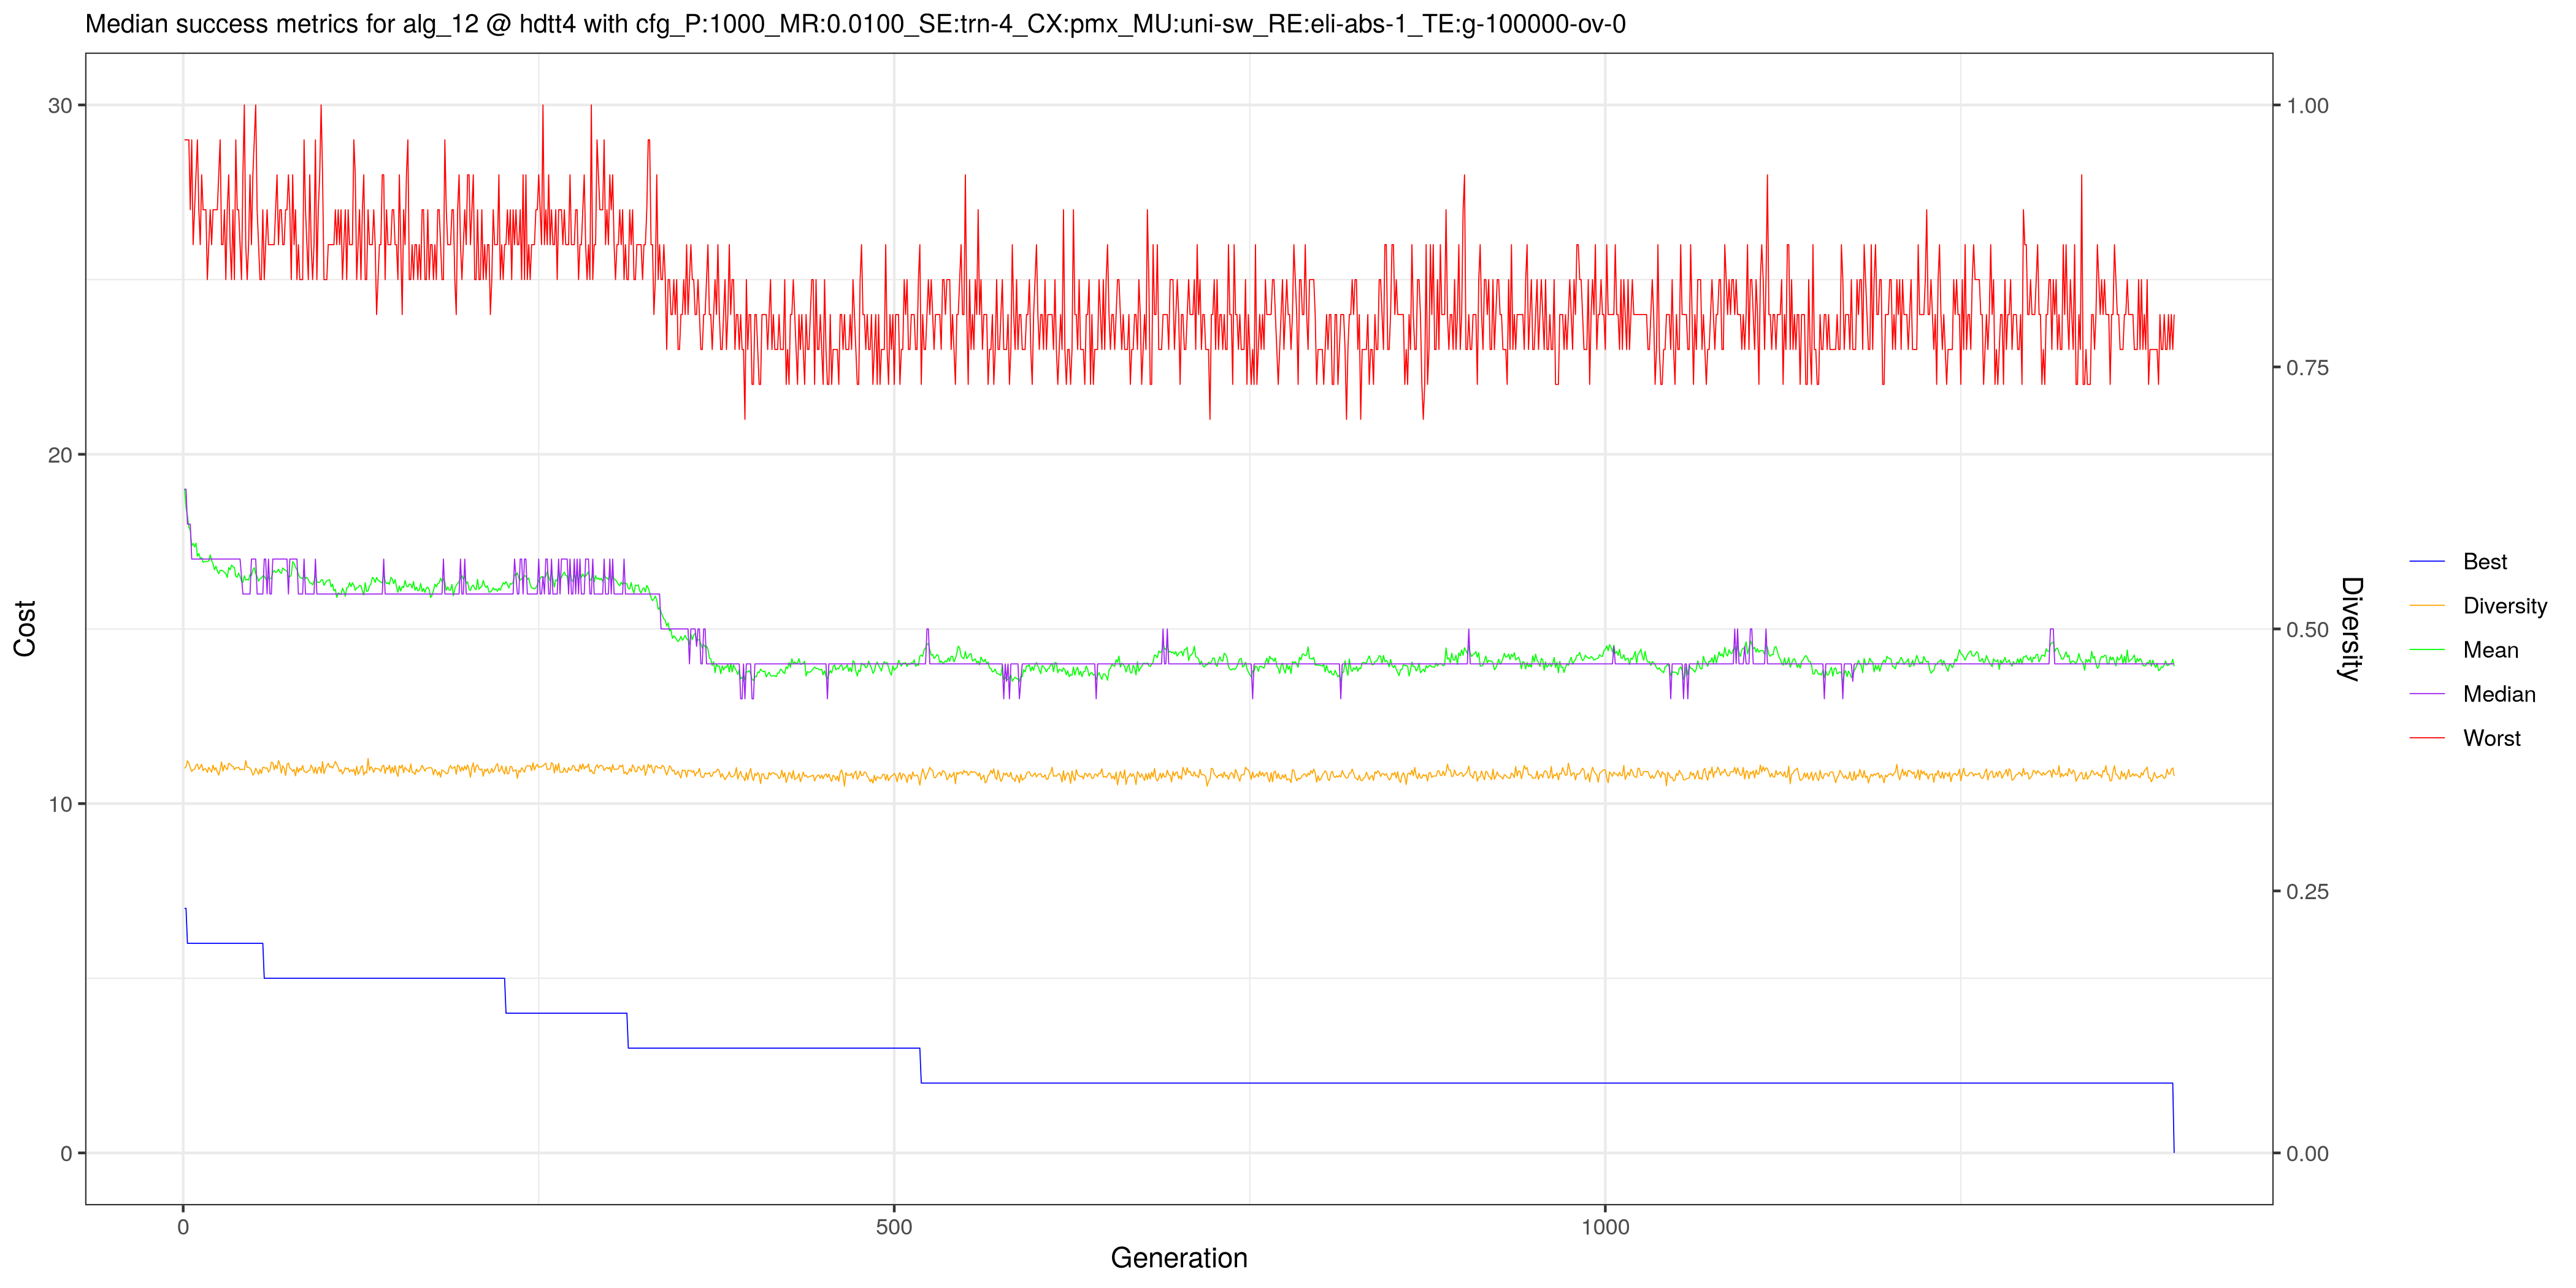
\includegraphics[width=1.28\textwidth]{assets/chap-7/discussion_1/hdtt4/alg_12/indirect_static_succ_median.png}
        \caption{
            Runtime metrics of \texttt{alg\_12} during a successful run
            solving \textit{hdtt4}.
        }
        \label{fig:hdtt4_alg12_indirect_static_succ_median}
    \end{adjustwidth}
\end{figure}
%
\begin{figure}[h]
    \begin{adjustwidth}{-3cm}{-3cm}
        \centering
        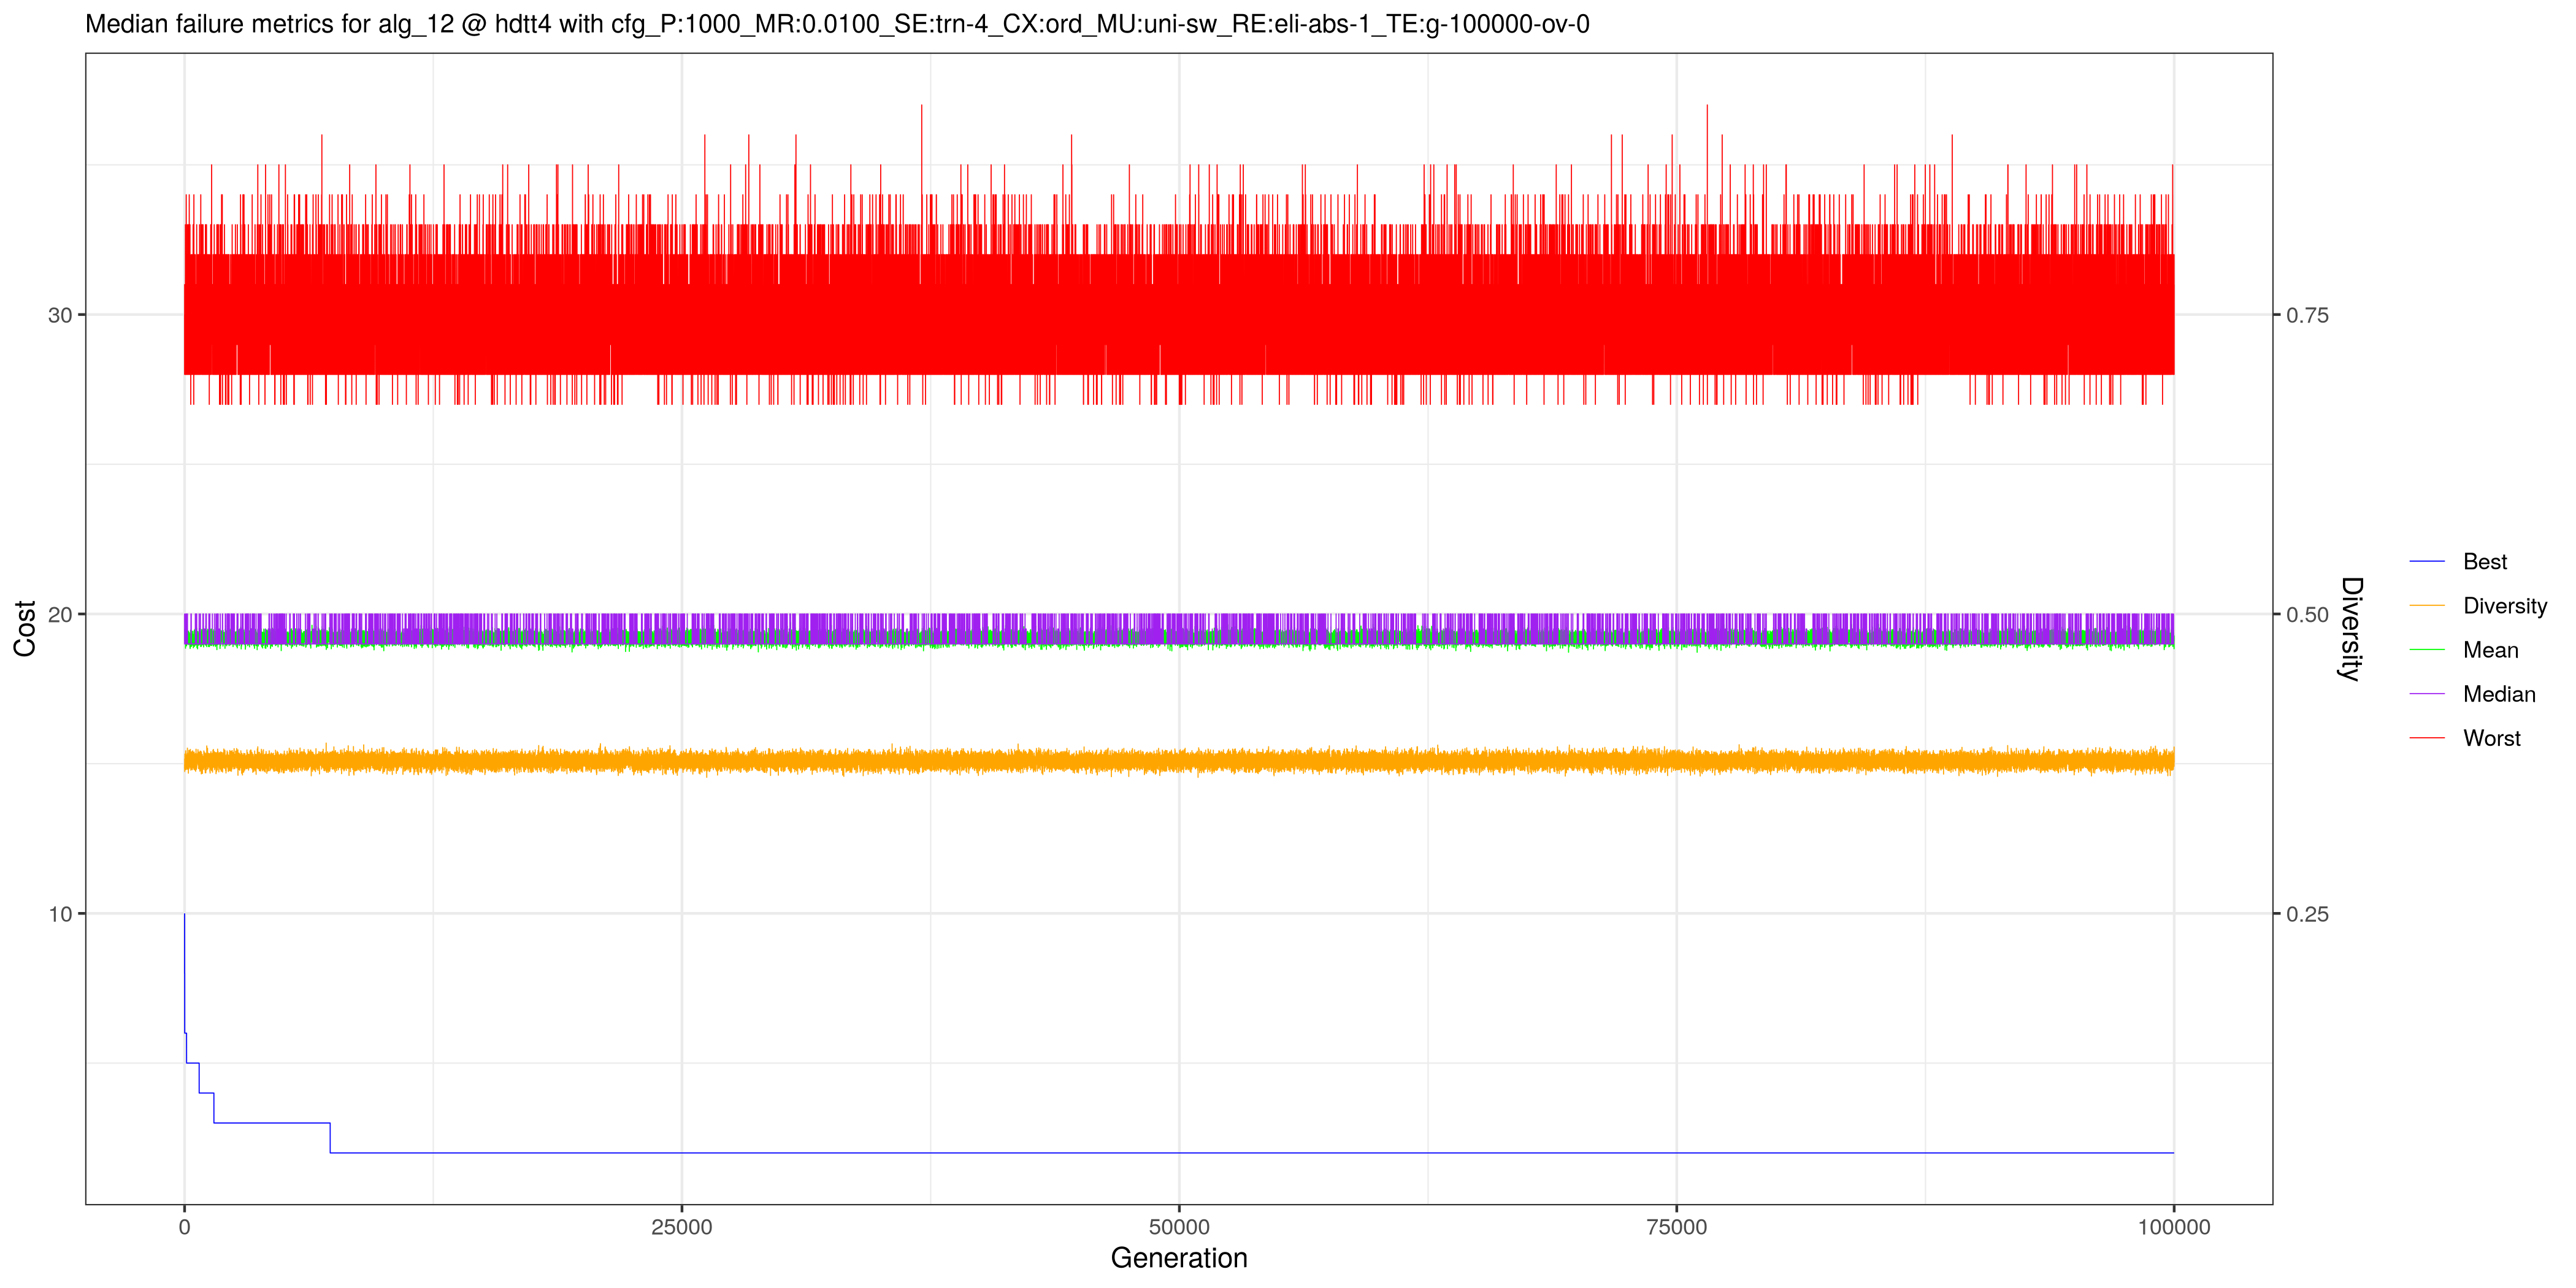
\includegraphics[width=1.28\textwidth]{assets/chap-7/discussion_1/hdtt4/alg_12/indirect_static_fail_median.png}
        \caption{
            Runtime metrics of \texttt{alg\_11} with self-parameterization
            during an unsuccessful run solving \textit{hdtt4}.
        }
        \label{fig:hdtt4_alg12_indirect_static_fail_median}
    \end{adjustwidth}
\end{figure}
%
Figures \ref{fig:hdtt4_alg12_indirect_static_succ_median} and
\ref{fig:hdtt4_alg12_indirect_static_fail_median} illustrate median successful
and unsuccessful runs of \texttt{alg\_12} without self-parameterization,
enabling a direct comparison to find indications of weaknesses in the direct
encoding scheme.

\subsection{Static Configuration}
Similar to the behavior observed with direct encoding, the diversity metric
of \texttt{alg\_12} in figure \ref{fig:hdtt4_alg12_indirect_static_succ_median}
remains almost constant or declines slowly over time, with no significant
spikes or changes in other metrics unless a better solution is discovered.
However, one stark difference, compared to \texttt{alg\_11}, is the much
faster convergence observed with indirect encoding. Algorithm \texttt{alg\_12}
consistently finds solutions in significantly fewer generations, reflecting the
efficiency of this encoding scheme in exploring the solution space.

For completeness, figure \ref{fig:hdtt4_alg12_indirect_static_fail_median}
depicts an unsuccessful run of the algorithm with indirect encoding using a
static configuration. Importantly, this visualization is based on a different
configuration than figure \ref{fig:hdtt4_alg12_indirect_static_succ_median},
as the configuration in this figure reliably succeeded across all executions.
Despite the configuration difference, the overall trends remain comparable to
those seen in successful runs. The diversity metric continues its slow decline
without notable spikes, indicating the absence of any dynamic influence on the
population's exploratory capabilities.

\subsection{Key Observations: Direct vs. Indirect Encoding}
While static configurations for \texttt{alg\_12} exhibit similar overall
behavior to those of \texttt{alg\_11}, certain distinctions are worth
emphasizing. First, even under static configurations, the diversity metric
of the indirect encoding is significantly higher than for the direct encoding.
This indicates that populations in the indirect encoding explore a broader
range of the solution space, even in the absence of parameter dynamics. Such
broader exploration inherently reduces the risk of premature convergence,
enabling the algorithm to achieve perfect reliability for multiple
configurations without requiring self-parameterization.

Second, there are notable differences in the distribution of objective values
across the population. With direct encoding, the best and median objective
values are often equal throughout the run, except for occasional spikes in the
median value. Simultaneously, the mean objective value consistently lags behind
the median. This indicates a distribution of objective values throughout
the population, which is significantly skewed towards the best objective value.
The imbalance of objective values and the resulting lack of diversity suggests
that populations of the direct encoded algorithm tend to converge prematurely,
resulting in populations that are tightly clustered around the best individuals,
which aligns with the observations made previously.

In \texttt{alg\_12}, however, the situation is markedly different.
The mean and median objective values are much closer to each other, with the
median seemingly aligned to the closest whole number to the mean.
Both the mean and median values remain significantly distinct from the best
% and worst objective value, by laying in the middle of them, representing a
objective value, representing a
well-distributed population.
Additionally, the relative positioning of the median and mean values provides
further evidence of greater population diversity.
For indirect encoding, the median objective value consistently occupies a
central position between the best and worst, unlike the skewed clustering
observed with direct encoding. This balanced diversity fosters reliability and
significantly reduces the risk of premature convergence, as demonstrated by
the perfect success rates achieved with static configurations.

\subsection{Dynamic Configuration (Self-Parameterization)}
\begin{figure}[h]
    \begin{adjustwidth}{-3cm}{-3cm}
        \centering
        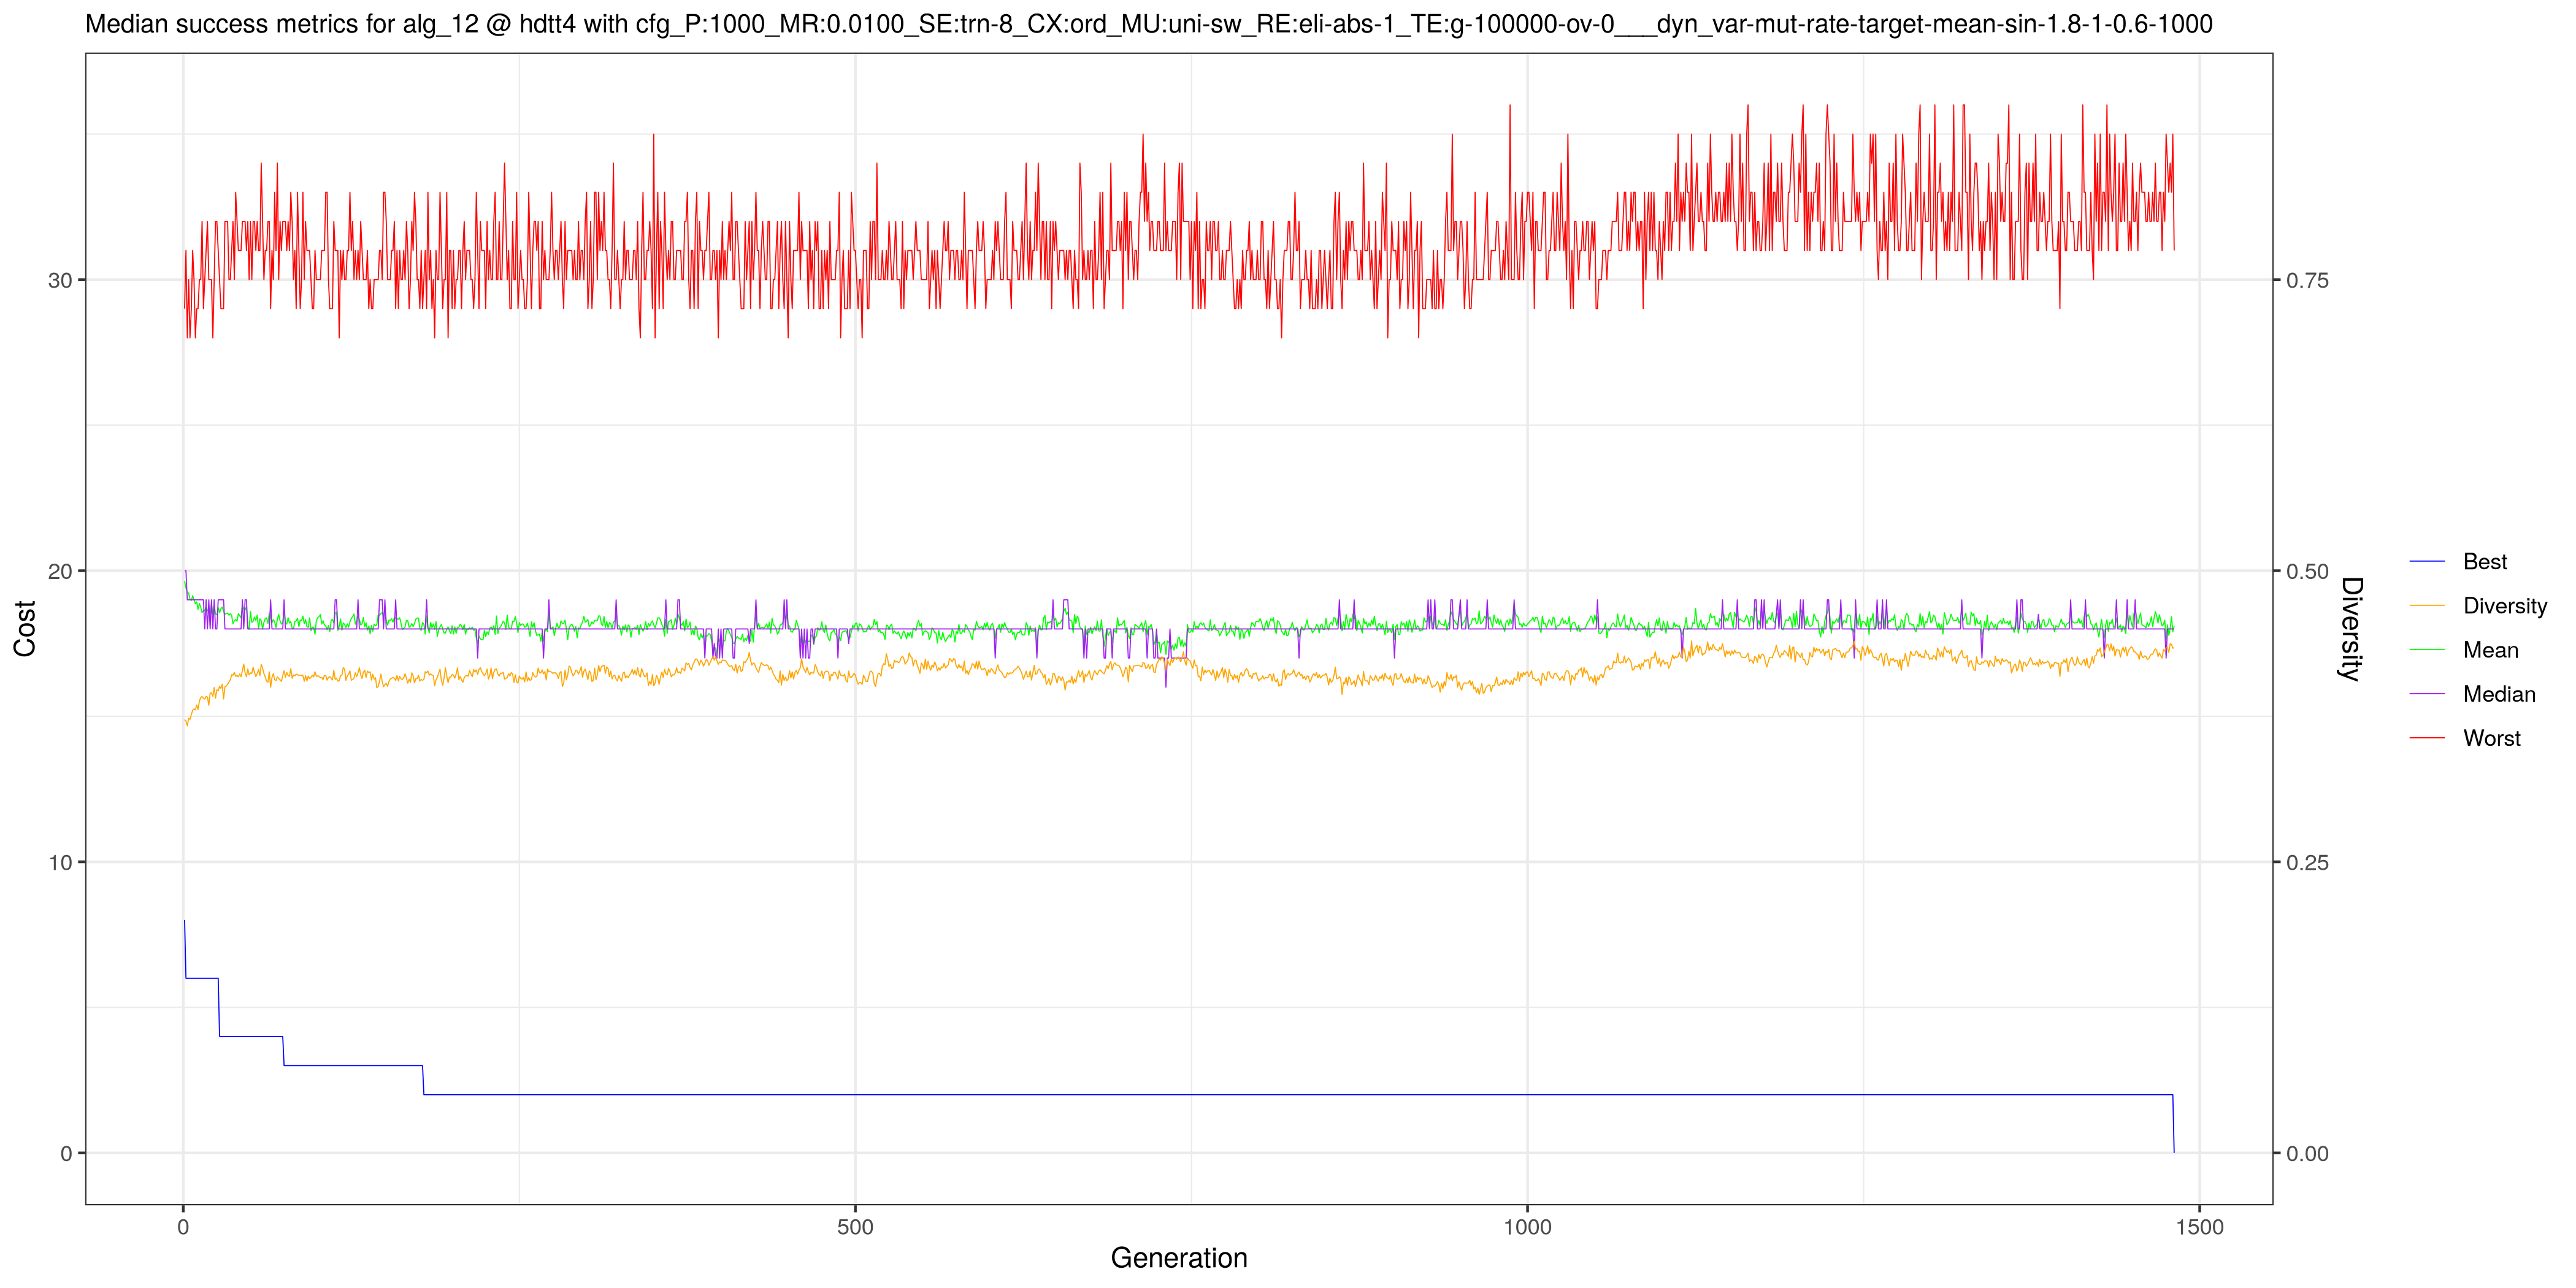
\includegraphics[width=1.28\textwidth]{assets/chap-7/discussion_1/hdtt4/alg_12/indirect_dynamic_succ_median.png}
        \caption{
            Runtime metrics of \texttt{alg\_12} with self-parameterization
            during a successful run solving \textit{hdtt4}.
        }
        \label{fig:hdtt4_alg12_indirect_dynamic_succ_median}
    \end{adjustwidth}
\end{figure}
Figure \ref{fig:hdtt4_alg12_indirect_dynamic_succ_median} illustrates a
successful run of \texttt{alg\_12} employing the
\textit{VarMutRateTargetMeanSin} dynamic (see \ref{VarMutRateTargetMeanSin}),
one of the most sophisticated self-parameterization techniques explored in this
study. This dynamic demonstrates the profound impact of adaptive parameter
adjustments on population metrics, particularly diversity. The plot reveals a
constantly evolving diversity metric, showcasing the ability of this dynamic to
actively steer the population away from stagnation

The dynamic's influence is especially pronounced in the final third of the
execution. As diversity begins to increase, the corresponding rise in the
worst objective value suggests that the algorithm is broadening its exploratory
search. This increased exploration ultimately leads to the discovery of an
optimal solution, as evidenced by the eventual reduction of the best objective
value to zero.

\subsection{Summary}
The comparison of \texttt{alg\_12} with static and dynamic configurations
reinforces the advantages of indirect encodings for genetic algorithms applied
to timetabling problems. Even without self-parameterization, the broader
diversity inherent in the indirect encoding approach reduces the likelihood
of premature convergence, enabling the algorithm to achieve perfect reliability
for multiple configurations. However, the addition of self-parameterization
further enhances the algorithm's exploration of the search space by dynamically
adapting to population metrics, albeit not resulting in any significant
differences regarding the algorithm's success rate or convergence speed.
These findings highlight the adaptability and robustness of indirect encoding
in combination with self-parameterization, making it a compelling choice for
solving complex timetabling problems.

%%% Insights %%%%%%%%%%%%%%%%%%%%%%%%%%%%%%%%%%%%%%%%%%%%%%%%%%%%%%%%%%%%%%%%%%%
\section{Insights}
While the preceding sections focus on discussing the observed results and
their immediate implications, this section delves deeper into the underlying
reasons behind the observed behaviors. It aims to provide a more theoretical
understanding of why the algorithms performed the way they did, offering
insights that go beyond the quantitative results. This allows for a focused
exploration of the mechanics of the encoding schemes and self-parameterization
techniques, addressing critical questions raised by the results.

\subsection{Challenges with Direct Encoding}
One of the most prominent observations from the results is that the direct
encoding algorithm requires self-parameterization to reliably solve the
high-school timetabling problems. Without these dynamic adjustments, the
algorithm consistently struggles with premature convergence, becoming trapped
in local maxima and failing to explore the search space effectively.

This behavior can be attributed to the nature of the crossover and mutation
operators used in the direct encoding algorithm.
Specifically, the trade crossover and mutation methods employed in this study
are derived from local search strategies (\cite{demiroBitvec,Fonseca2014}; as
mentioned in chapter \ref{n-trade crossover}).
While these operators were carefully adapted to ensure they produce valid
timetables by making meaningful changes to the chromosomes in the context of
timetabling, their design inherently prioritizes incremental improvements.
This makes them highly effective in refining solutions locally, but may be less
suited to making exploratory leaps that escape local maxima. For instance,
these operators often generate offspring whose objective values closely
resemble those of their parents, which aligns well with the principles of
local search, and corresponds to the skewed distribution of objective values
observed previously, but limits broader exploration.

Incorporating self-parameterization allows the algorithms to counteract this
limitation. Dynamic adjustments to parameters, as demonstrated with the
state machine method, periodically disrupt the algorithm's convergence
trajectory. These disruptions introduce additional diversity into the
population, providing the algorithm with the flexibility to escape local maxima
and discover new regions of the solution space, as demonstrated by the
state machine self-parameterization method which temporarily disables
elitist replacement to introduce diversity and thereby enables broader
exploration.

However, while this approach proved effective for \textit{hdtt4}, the results
show that \texttt{alg\_11} could not solve the \textit{hdtt5} problem instance
with any of the tested configurations and dynamics. The reason lies in the
increased complexity of this instance. As the problem grows more complex, the
algorithm converges less rapidly due to the expanded search space and requires
longer exploration phases. In such cases, the periodic resets introduced by
the state machine dynamic may disrupt the algorithm prematurely, preventing
it from thoroughly exploring promising regions of the search space before
being set back. This suggests that while self-parameterization is crucial for
overcoming the challenges of the developed direct encoding, the specific
implementation of self-parameterization must scale with the complexity of the
problem instance to remain effective.

This interplay between algorithmic dynamics and problem complexities underscores
the delicate balance required in designing effective self-parameterization
techniques for direct encoding approaches.

\subsection{Characteristics of Indirect Encoding}
In contrast to the direct encoding, the indirect encoding algorithm exhibits
faster convergence and does not significantly benefit from
self-parameterization. These differences stem from the fundamental properties
of the indirect encoding scheme and the heuristic used to map genotypes
to phenotypes.

Unlike the direct encoding, where each genotype corresponds to a single
phenotype, the indirect encoding represents solutions in a more abstract form,
namely a sequence of scheduling operations.
The representation of a potential solution as a sequence the events must be
scheduled, does not \textit{unambiguously} represent a timetable.
Conversely, multiple timetables (phenotypes) can be derived from one genotype,
as the genotype only dictates the order in which the events must be scheduled,
but not the time slots each event should be allocated at.
This allocation is performed by a heuristic algorithm. The heuristic employed
in this study selects a specific phenotype for each genotype based on a
predefined set of rules designed to produce high-quality solutions.
For example, the heuristic ensures that resource conflicts are entirely avoided
in the generated timetables.

This heuristic-driven mapping introduces a dual effect. On one hand, it
accelerates convergence by consistently generating high-quality phenotypes.
Even though the indirect encoding has to navigate a larger search space due
to its permutation-based chromosome structure, the heuristic's ability to
prioritize valid and fit solutions allows the algorithm to explore this space
efficiently. This explains the observed rapid convergence of \texttt{alg\_12},
even in the absence of self-parameterization.

On the other hand, the heuristic's focus on producing specific phenotypes limits
the algorithm's ability to explore the full solution space. By skipping over
a significant portion of potential timetables, which are sorted out by the
heuristic, the algorithm risks overlooking optimal or near-optimal solutions.
This limitation becomes apparent in scenarios where \texttt{alg\_12} does not
find a viable timetable.
The self-parameterization techniques implemented in this study do not address
this issue because the heuristic was not designed to be externally
parameterized so that self-parameterization methods could influence it.
As a result, while self-parameterization improves diversity and search dynamics,
it cannot overcome the inherent constraints imposed by the heuristic-driven
mapping.

These insights highlight the trade-offs associated with the indirect encoding
approach. While it offers faster convergence and high-quality solutions in many
cases, its reliance on a heuristic limits its adaptability and leaves some
parts of the solution space unexplored.


%%%%%%%%%%%%%%%%%%%%%%%%%%%%%%%%%%%%%%%%%%%%%%%%%%%%%%%%%%%%%%%%%%%%%%%%%%%%%%%%
%%% 8. Conclusion                                                            %%%
%%%%%%%%%%%%%%%%%%%%%%%%%%%%%%%%%%%%%%%%%%%%%%%%%%%%%%%%%%%%%%%%%%%%%%%%%%%%%%%%
\chapter{Conclusion}
This thesis explores the application of adaptive evolutionary techniques in
genetic algorithms for solving high-school timetabling problems, focusing on
the impact of self-parameterization methods. Through extensive experimentation,
several key insights were gained.

Firstly, the study demonstrates that self-parameterization methods do not
universally enhance the performance of genetic algorithms. Their effectiveness
depends heavily on the encoding scheme employed. While the direct encoding
benefited significantly from dynamic adjustments, the indirect encoding showed
limited improvement, with certain configurations even performing worse when
self-parameterization was applied. This finding underscores the necessity
of tailoring adaptive techniques to the specific characteristics of the
encoding, as the analyzation of the indirect encoding indicates, that
parameterizing the heuristic method and therefore dynamically adapting the
indirect encoding's exploration characteristics is a promising application
of self-parameterization even for this kind of encoding.

Secondly, the choice of self-parameterization methods and their associated
parameters introduces a new layer of complexity to genetic algorithm design.
These methods, while aimed at reducing the need for manual parameter tuning,
are themselves subject to the parameter tuning problem. For instance, the
state machine dynamic demonstrated its capability to escape local maxima in the
direct encoding algorithm. However, its periodic resets were less effective
for the more complex \textit{hdtt5} problem instance, suggesting that the
effectiveness of such techniques is highly context-dependent.

To address this challenge, future research should focus on designing adaptive
evolution techniques that minimize manual intervention while maintaining
robustness across diverse problem instance. Achieving this will likely require
analyzing the behavior of genetic algorithms on a broad range of instances to
identify patterns and develop advanced strategies. Such strategies may involve
complex models capable of autonomously adjusting parameters based on runtime
metrics and population dynamics.

Additionally, this thesis contributed open-source implementations and a
practical genetic algorithm framework for facilitating future research.
The developed framework for implementing genetic algorithms offers a robust,
foundation for experimentation. By including metrics collection and real-time
logging capabilities, as well as providing a standardized interface for
self-parameterization techniques, this framework paves the way for future
exploration of genetic algorithms in timetabling and beyond.
The source code of the presented algorithms, the genetic algorithm framework
and all the collected data of algorithm executions are openly available
on GitHub, ensuring transparency, reproducibility and enabling other
researchers to build upon this work (\cite{code-gax,code-gax-plots}).

While this study advances the understanding of adaptive evolutionary techniques,
certain limitations remain. The algorithms were tested on only two problem
instances, limiting the generalizability of the findings. Furthermore, the
methods of self-parameterization, though diverse, represent just a subset of
potential methods. Addressing these limitations could significantly enhance the
impact and applicability of this research.

In conclusion, this thesis highlights both the promise and the challenges of
self-parameterizing genetic algorithms. It provides a stepping stone toward
more robust and versatile algorithms while emphasizing the importance of
encoding-specific design and thorough analysis of parameter dynamics.


%%%%%%%%%%%%%%%%%%%%%%%%%%%%%%%%%%%%%%%%%%%%%%%%%%%%%%%%%%%%%%%%%%%%%%%%%%%%%%%%
%%% 9. Future Work                                                           %%%
%%%%%%%%%%%%%%%%%%%%%%%%%%%%%%%%%%%%%%%%%%%%%%%%%%%%%%%%%%%%%%%%%%%%%%%%%%%%%%%%
\chapter{Future Work}
This thesis lays the groundwork for future advancements in the application of
genetic algorithms to high-school timetabling and highlights several areas
where further exploration could enhance both the effectiveness and
generalizability of the algorithms.

One promising direction for future research is to extend the algorithms'
ability to solve a broader range of problem instances.
The current study focused on two relatively small instances to establish
baseline functionality and reliability.
Tackling more complex timetabling problems, particularly those involving
advanced constraints, would not only test the robustness of the existing
approaches but also drive the development of more sophisticated encoding
schemes and operators.

For the direct encoding, an intriguing possibility lies in revisiting its
data structures. Currently, the genotype and phenotype use
\lstinline[language=Rust]{Vec<Bits32>} and
\lstinline[language=Rust]{Vec<Bits64>} for storing and processing timetabling
information. Transitioning to matrix types (e.g.,
\lstinline[language=Rust]{BitsMatrix32x128}), which were originally developed
to improve the performance of the computationally more intensive indirect
encoding, might offer similar performance gains for the direct encoding.
Evaluating this change could reveal whether it significantly accelerates the
algorithm's execution without the necessity to alter the core logic of the
encoding.

Additionally, testing static configurations of the direct encoding with a wider
range of parameter values could yield further insights. This would provide a
more comprehensive understanding of how static setups compare to their dynamic
counterparts and identify potential areas for optimization.

For the indirect encoding, future studies could investigate altering the
\enquote{focal length} of its genotype-to-phenotype mapping.
Currently, the heuristic mapping prioritizes certain features of the solution
space, which leads to faster convergence but potentially skips over regions
containing optimal solutions.
Adjusting this focus -- either statically or dynamically -- could reveal new
trade-offs between exploration and exploitation.
Moreover, self-parameterization techniques specifically targeting the
genotype-to-phenotype mapping process might allow for more nuanced adjustments
during runtime, further enhancing the algorithm's adaptability.

In summary, future work could explore extending the range of solvable problem
instances, developing advanced self-parameterization strategies, optimizing
data structures, and refining the encoding schemes. By addressing these
areas, researchers can build on the foundations established in this thesis
to create more powerful, versatile and efficient genetic algorithms for
more complex high-school timetabling instances.



%%%%%%%%%%%%%%%%%%%%%%%%%%%%%%%%%%%%%%%%%%%%%%%%%%%%%%%%%%%%%%%%%%%%%%%%%%%%%%%%
% Bibliography
\bibliographystyle{plain}%{alpha}
\bibliography{thesis}

% Declaration of Academic Honesty
\makedeclaration

\end{document}

%%%%%%%%%%%%%%%%%%%%%%%%%%%%%%%%%%%%%%%%%%%%%%%%%%%%%%%%%%%%%%%%%%%%%%%%%%%%%%%%
